\documentclass[a4paper,titlepage,UTF8]{ctexbook}

% 导言区

\usepackage[colorlinks, linkcolor=blue!50!black]{hyperref} 

\usepackage{xcolor}
\usepackage{listings}
\usepackage{geometry}
\usepackage{fancyhdr}
\usepackage{cite}
\usepackage[super]{gbt7714} % 中文文献包
\usepackage{graphicx} % 导入图片包
\graphicspath{{img/game/},{img/install/},{img/screenfetch/}}
\usepackage{subfig}
\usepackage{tabularx}
\usepackage{chngpage}
\usepackage{array}
\usepackage{parskip}
\usepackage{booktabs}
\usepackage{longtable}
\usepackage{makecell} % 表格
\usepackage{pbox}
\usepackage{graphicx} % 导入图片包
\graphicspath{{img/}}
\usepackage[bodytextleadingratio=1.45]{zhlineskip}
\usepackage{paralist}
\usepackage{adjustbox}
\usepackage{lstfiracode}
\usepackage{minted}
\usepackage[normalem]{ulem} % 定义文本高亮
% 定义需要强调的环境
\newenvironment{notice}[1][注意]{{\textbf{#1}:}}

\newenvironment{seeAlso}[1][另请参阅]{{\textbf{#1}:}}

\newenvironment{warning}[1][警告]{{\textbf{#1}:}}

% 定义文本高亮
\newcommand\hl{\bgroup\markoverwith
  {\textcolor{yellow}{\rule[-.5ex]{2pt}{2.5ex}}}\ULon}

% 定义分隔线的样式
% \dotfill: 虚线
% \hrulefill: 实线
\newcommand{\splitLine}{\dotfill}

% 行内高度
\newcommand{\lineHigh}{\vspace{2em}}

% 不输出标题编号
\newcommand\specialsectioning{\setcounter{secnumdepth}{-1}}
\ctexset{section/format += \raggedright}

% \newfontfamily\consolas{Fira Code}
\newfontfamily\consolas{Source Code Pro}
% \newfontfamily\consolas{JetBrainsMono-Regular}

% green
\definecolor{mygreen}{rgb}{0, 0.6, 0}

% 页边距
\geometry{left=2.5cm,right=2.5cm,top=2.0cm,bottom=2cm}

% 页眉页脚
\pagestyle{empty}

% 设定代码环境
\newfontfamily\fira{Fira Code}
\lstset{
	basicstyle=\small\fira,
	numberstyle= \tiny\fira, 
	keywordstyle= \color{ blue!70},
	commentstyle=\color{mygreen},
	frame=shadowbox, 
	rulesepcolor= \color{ red!20!green!20!blue!20},
	columns=flexible, 
	linewidth=1.1\linewidth,
} 


% 定义表格列宽
\newcolumntype{L}[1]{>{\vspace{0.5em}\begin{minipage}{#1}\raggedright\let\newline\\
\arraybackslash\hspace{0pt}}m{#1}<{\end{minipage}\vspace{0.5em}}}
\newcolumntype{R}[1]{>{\vspace{0.5em}\begin{minipage}{#1}\raggedleft\let\newline\\
\arraybackslash\hspace{0pt}}m{#1}<{\end{minipage}\vspace{0.5em}}}
\newcolumntype{C}[1]{>{\vspace{0.5em}\begin{minipage}{#1}\centering\let\newline\\
\arraybackslash\hspace{0pt}}m{#1}<{\end{minipage}\vspace{0.5em}}}

% 中文设置
\setCJKmainfont{SourceHanSerifCN-Light}

% 英文设置
% \setmainfont{JetBrains Mono}
\setmainfont{Source Code Pro}

% 标题页
\title{Qt中文文档翻译}
\author{作者:\href{https://github.com/QtDocumentCN}{QtDocumentCN}}
\CTEXoptions[today=small]
 % 标题左对齐
\CTEXsetup[format={\Large}]{section}
% \ctexset{ section = {format = {\Large}}

% 首行缩进两个字符
%\setlength{\parindent}{2em}
%\CTEXindent 
\CTEXnoindent % 取消首行缩进

\setlength{\headheight}{20pt}

\begin{document}
% 正文区(文稿区)
% 页眉页脚
\pagestyle{fancy}
\lhead{\includegraphics[scale=0.1]{logo}}
\renewcommand{\headrulewidth}{0.4pt}

\maketitle

\thispagestyle{empty}
\clearpage
\setcounter{page}{1}

\clearpage
% \newgeometry{top=0in}
\tableofcontents
% \restoregeometry
\clearpage

\setcounter{page}{1}

% 不输出标题编号
\specialsectioning

\chapter{API Design Principles}

API 设计规范

\begin{quote}
译者注:

本文不来自于 Qt 文档,而是来自于 Qt Wiki:\href{https://wiki.qt.io/API_Design_Principles}{API\_Design\_Principles}

API(Application Programming Interface),应用开发接口,本文中也将 P 解释为 Programmer(开发者)。	
\end{quote}

Qt 最出名的特点之一是一致性强、易于学习、功能强大的 API。本文尝试对我们在设计 Qt 风格的 API 中积累的诀窍进行总结。其中许多准则都是通用的,其它的则是习惯性用法,我们主要为了保持接口一致性而继续遵循。

尽管这些准则主要面向公共接口,但也鼓励您在设计内部接口时使用相同的技术,这对与您合作开发的同僚会更加友好。

您可能也会有兴趣查阅 Jasmin Blanchette 的 
\href{https://people.mpi-inf.mpg.de/~jblanche/api-design.pdf}{Little Manual of API Design (PDF)},或它的前身,由 Matthias Ettrich 编写的 \href{https://doc.qt.io/archives/qq/qq13-apis.html}{Designing Qt-Style C++ APIs} 。

优秀接口的六大特点

API 是面向开发者的,而 GUI 则是面向终端用户。API 中的 P 代表开发者(Programmer),而非程序(Program),目的是指出 API 由开发者,即人类(而非计算机)所使用这一特点。

Matthias 在 Qt 季刊弟13期,关于 API 设计的文章中,声称他坚信 API 应该是最小化但完备的,具备清晰而简洁的语义,符合直觉,被开发者,易于记忆,能够引导开发者编写高可读性的代码。

最小化

最小化的 API 指包含尽可能少的公共成员和最少的类。这可让 API 更易于理解、记忆、调试和修改。

完备性
完备的 API 意味着具备所有应有的功能。这可能会与最小化产生冲突。此外,若一个成员函数位于错误的类中,则大多数潜在的用户回无法找到它。

清晰简洁的语义

与其它设计协作时,应该让您的设计做到最小例外。通用化会让事情更简单。特例可能存在,但不应成为关注的焦点。在处理特定问题时,不应让解决方案过度泛化。(例如,Qt 3 中的 QMineSourceFactory 本该被称作 QImageLoader,并且具备另一套 API。)

复合直觉

如同计算机上其它内容,API 应复合直觉。不同的开发经验和技术背景会导致对复合直觉与否有不同的感知。复合直觉的 API 应能让中等经验的开发者无需阅读文档并直接使用,并让不知道这个 API 的开发者可以理解使用它编写的代码。

易于记忆

为了让 API 易于记忆,请选择一组保持一致并足够精确的命名约定。使用可理解的模式和概念,并且避免缩写。

可读性导向

编写代码只需要一次,但阅读(以及调试和修改)则会非常频繁。高可读性的代码通常需要花更多时间编写,但可以在产品的生命周期中节约更多的时间。

最后需要谨记,不同类型的用户会使用 API 的不同部分。在单纯地创建一个 Qt 类实例能非常直观的同时,希望用户在尝试继承它之前先阅读文档则是很合理的。

静态多态

相似的代码类应具有相似的 API。可以使用继承来实现——当运行时多态支持时,这是很合理的。但多态同时也可以体现在设计截断。例如,若将代码中的 QProgressBar 换为 QSlider,或将 QString 换为 QByteArray,他们间相似的 API 会另替换操作变得非常容易。这便是为何我们称之为“静态多态”。

静态多态同样可让记忆 API 和开发模式变得更加简单。结果是,对于一组有关联的类,相似的 API 通常比为每个类独立设计的完美 API 更加好用。

在 Qt 中,当不具备有足够说服力的原因时,我们更倾向于使用静态多态,而非继承。这减少了 Qt 的公共类数量,并让新用户更容易在文档中找到需要的内容。

好的

​ QDialogBox 和 QMessageBox 具有相似的 APi,以用于处理按钮(addButton(), setStandardButtons(),但无需继承自某些 "QAbstractButtonBox" 类。

坏的

​ QAbstractSocket 被 QTcpSOcket 和 QUdpSocket 所继承,但这两个类的交互方式差异很大。看起来并没有人使用过(或能够使用) QAbstractSocket 指针来进行通用且有效的操作。

存疑

​ QBoxLayout 是 QHBoxLayout 和 QVBoxLayout 的基类。优点:可以在工具栏中使用 QBoxLayout,调用 setOrientation() 来令其水平/垂直排布。缺点:引入额外的类,用户可能会写出形如 ((QBoxLayout *)hbox)->setOrientation(Qt::Vertical) 的代码,而这是不合理的。

基于属性的 API
比较新的 Qt 类倾向于使用基于属性的 API,例如:

\begin{lstlisting}
QTimer timer;
timer.setInterval(1000);
timer.setSingleShot(true);
timer.start(); 
\end{lstlisting}

此处的属性,指的是作为对象状态一部分的任何概念性的特征——无论是否是实际的 Q\_PROPERTY。只要可行,用户都应该允许以任何顺序设置属性,也就是说,这些属性应该是正交的。例如,上文的代码也可以写为:

\begin{lstlisting}
QTimer timer;
timer.setSingleShot(true);
timer.setInterval(1000);
timer.start(); 
\end{lstlisting}

为了方便,我们也可以这样写:

\begin{lstlisting}
timer.start(1000);
\end{lstlisting}

类似的,对于 QRegExp,我们可以:

\begin{lstlisting}
QRegExp regExp;
regExp.setCaseSensitive(Qt::CaseInsensitive);
regExp.setPattern(".");
regExp.setPatternSyntax(Qt::WildcardSyntax);
\end{lstlisting}

为了实现此类 API,内部的对象需要被惰性构造。例如在 QRegExp 的案例中,不应该在还不知道表达式使用何种语法之前,就在 setPattern() 中过早地编译 . 表达式。

属性通常是级联的,此时我们应该谨慎地处理。仔细考虑下当前样式提供的“默认图标大小”与 QToolButton 的 iconSize 属性:

\begin{lstlisting}
toolButton->iconSize(); // 返回当前样式表的默认大小
toolButton->setStyle(otherStyle);
toolButton->iconSize(); // 返回 otherStyle 的默认大小
toolButton->setIconSize(QSize(52, 52));
toolButton->iconSize(); // 返回 (52, 52)
toolButton->setStyle(yetAnotherStyle);
toolButton->iconSize(); // 返回 (52, 52) 
\end{lstlisting}


注意,一旦 iconSize 被设置,它会被一直留存,此时修改当前样式不会影响它。这是 好的。有时,提供重置属性的渠道会很方便,这有两种实现方式:

\begin{itemize}
	\item 传递一个特定值(如 QSIze()、-1 或 Qt::Alignment(0))来指代“重置”;
	\item 提供显示的 resetFoo() 或 unsetFoo() 函数。
\end{itemize}

对于 iconSize,将 QSize()(即 QSize(-1, -1))设为“重置”便足够了。

某些场景中,取值方法会返回值会与设置的内容不同。例如,若调用 widget->setEnabled(true),可能通过 widget->isEnabled() 获得的依然是 false,因为父控件被禁用了。这并没问题,因为通常这正是我们要检查的状态(父控件被禁用时,子控件也应该变灰,表现为也被禁用,但同时在它内部,应该知道自己实际是“可用”的,并等待父控件可用后恢复状态),但必须在文档中正确地进行描述。

QProperty

\begin{quote}
译者注:该类型为 Qt 6.0 引入,需要参见 Qt 6 类文档。

本文原文中的内容与现有的 Qt 6.0 预览版存在出入,因此暂不翻译本节,待官方进一步维护更新原文。
\end{quote}

C++ 特性

值 与 对象

\begin{quote}
译者注:此条原文无内容,待官方更新
\end{quote}

指针 与 引用

作为输出参数,指针与引用哪个更好?

\begin{lstlisting}
void getHsv(int *h, int *s, int *v) const void getHsv(int &h, int &s, int &v) const
\end{lstlisting}

绝大多数 C++ 数据都推荐尽可能使用引用,因为引用在感知上比指针“更安全更漂亮”。事实上,我们在 Qt 软件中更倾向于使用指针,因为这会令代码更加已读。如对比:

\begin{lstlisting}
color.getHsv(&h, &s, &v);
color.getHsv(h, s, v);
\end{lstlisting}

第一行代码能很清晰地表示,h、s、v 对象有很大概率会被该函数调用所修改。

即便如此,由于编译器并不喜欢输出参数,在新 APi 中应该避免此用法,而是返回一个小结构体:

\begin{lstlisting}
struct Hsv { int hue, saturation, value }; Hsv getHsv() const;
\end{lstlisting}

\begin{quote}
	译者注:对于可能失败的带返回值的函数,Qt 倾向于返回数值,使用 bool* ok = 0 参数来存储调用结果,以便在不关心时忽略之。同样在 Qt 6 以后,该方式不再被建议使用,而是改用 std::optional<T> 返回类型。
\end{quote}

传递常引用 与 传递值
若类型大于16字节,传递常引用。

若类型具有非平凡的拷贝构造函数或非平凡的析构函数,传递常引用来避免执行这些方法。

所有其它类型都应使用值传递。

范例:

\begin{lstlisting}
void setAge(int age);
void setCategory(QChar cat);
void setName(QLatin1String name);
void setAlarm(const QSharedPointer<Alarm> &alarm); // 常引用远快于拷贝构造和析构
// QDate, QTime, QPoint, QPointF, QSize, QSizeF, QRect 都是其它应该值传递的好例子
\end{lstlisting}

虚函数

当 C++ 中的一个成员函数被声明为虚函数,这主要用于通过在子类中重写来自定义该函数的行为。将函数设为虚函数的目的是让对该函数的现有调用会被替代为访问自定义的代码分支。若在该类之外没人调用此函数,则在将其声明为虚函数之前需要小心斟酌:

\begin{lstlisting}
// Qt 3 中的 QTextEdit: 成员函数不需要作为虚函数的成员函数
virtual void resetFormat();
virtual void setUndoDepth( int d );
virtual void setFormat( QTextFormat &f, int flags );
virtual void ensureCursorVisible();
virtual void placeCursor( const QPoint &pos;, QTextCursorc = 0 );
virtual void moveCursor( CursorAction action, bool select );
virtual void doKeyboardAction( KeyboardAction action );
virtual void removeSelectedText( int selNum = 0 );
virtual void removeSelection( int selNum = 0 );
virtual void setCurrentFont( const QFont &f );
virtual void setOverwriteMode( bool b ) { overWrite = b; }
\end{lstlisting}




\chapter{QAbstractAnimation}

% \tocpart{QAbstractAnimation}

QAbstractAnimation 是所有的动画相关的基类。

QAbstractAnimation 定义了所有动画类相关的基础功能,通过继承该类,您可以实现动画的其它功能,或者添加自定义的特效。

\begin{tabular}{|r|l|}
	\hline
	属性 & 方法 \\
	\hline
	头文件 & \#include <QAbstractAnimation>\\      
	\hline
	qmake & QT+=core\\      
	\hline
	自从 & Qt 4.6\\
	\hline
	继承&QObject \\
	\hline
	派生 & QAnimationGroup,QPauseAnimation,QVariantAnimation \\
	\hline
\end{tabular}

\section{公共成员类型}

\begin{tabular}{|r|l|}
	\hline
	类型 & 方法 \\
	\hline
	enum & DeletionPolicy \{ KeepWhenStopped, DeleteWhenStopped \}\\      
	\hline
	enum & Direction \{ Forward, Backward \}\\      
	\hline
	enum & State \{ Stopped, Paused, Running \}\\
	\hline
\end{tabular}

\section{属性}

\begin{tabular}{|l|l|l|l|}
	\hline
	属性 & 类型 &属性 &类型 \\
	\hline
		currentLoop & const int &duration &const int \\
	\hline
	currentTime	&int&	loopCount&	int\\
	\hline
	direction	&Direction	&state&	const State\\
	\hline
\end{tabular}


\section{公共成员函数}

\begin{tabular}{|r|l|}

\hline
返回类型 &	函数名\\
\hline
& QAbstractAnimation(QObject \emph{*parent} = Q\_NULLPTR)\\
\hline
virtual&$\sim$QAbstractAnimation()\\
\hline
int	& currentLoop() const\\
\hline
int	& currentLoopTime() const\\
\hline
int	& currentTime() const\\
\hline
Direction& direction() const\\
\hline
virtual int	&duration() const = 0\\
\hline
QAnimationGroup *&	group() const\\
\hline
int	&loopCount() const\\
\hline
void&	setDirection(Direction \emph{direction})\\
\hline
void&	setLoopCount(int \emph{loopCount})\\
\hline
State&	state() const\\
\hline
int	& totalDuration() const\\
\hline
\end{tabular}

\section{公共槽}

\begin{tabular}{|r|l|}
\hline
返回类型&	函数名 \\
\hline
void&	pause()\\
\hline
void&	resume()\\
\hline
void&	setCurrentTime(int \emph{msecs})\\
\hline
void&	setPaused(bool \emph{paused})\\
\hline
void&	start(QAbstractAnimation::DeletionPolicy \emph{policy} = KeepWhenStopped)\\
\hline
void&	stop() \\
\hline
\end{tabular}
\chapter{QAbstractAudioDeviceInfo}

% \tocpart{QAbstractAudioDeviceInfo}

QAbstractAudioDeviceInfo 是音频后端的基类。

\begin{tabular}{|r|l|}
	\hline
	属性 & 方法 \\
	\hline
	头文件 & \#include <QAbstractAudioDeviceInfo>\\      
	\hline
	qmake & QT += multimedia\\      
	\hline
	继承&QObject \\
	\hline
\end{tabular}

\section{公共功能}

\resizebox{\textwidth}{!}{ % Latex表格宽度超出文本宽度
\begin{tabular}{|r|l|}
	\hline
	类型 & 方法 \\
	\hline
	virtual QString	 & deviceName() const = 0 \\
	\hline
	virtual bool &isFormatSupported(const QAudioFormat \&format) const = 0 \\
	\hline
	virtual QAudioFormat &	preferredFormat() const = 0\\
	\hline
	virtual QListQAudioFormat::Endian &	supportedByteOrders() = 0 \\
	\hline
	virtual QList &	supportedChannelCounts() = 0 \\
	\hline
	virtual QStringList&	supportedCodecs() = 0\\
	\hline
	virtual QList&	supportedSampleRates() = 0\\
	\hline
	virtual QList&	supportedSampleSizes() = 0\\
	\hline
	virtual QListQAudioFormat::SampleType&	supportedSampleTypes() = 0 \\
	\hline
\end{tabular}
}


\section{类型}

详细说明

QAbstractAudioDeviceInfo是音频后端的基类。

该类实现了QAudioDeviceInfo的音频功能,即QAudioDeviceInfo类中会保留一个QAbstractAudioDeviceInfo,并对其进行调用。关于QAbstractAudioDeviceInfo的实现的其它功能,您可以参考QAudioDeviceInfo的类与函数文档

\section{成员函数文档}

QString QAbstractAudioDeviceInfo::deviceName() const [纯虚函数] 

返回音频设备名称

bool QAbstractAudioDeviceInfo::isFormatSupported(const QAudioFormat \emph{\&format}) const [纯虚函数] 

传入参数QAudioFormat(音频流)类,如果QAbstractAudioDeviceInfo支持的话,返回true(真是不好翻译)

QAudioFormat QAbstractAudioDeviceInfo::preferredFormat() const [纯虚函数]

返回QAbstractAudioDeviceInfo更加倾向于使用的音频流。

QListQAudioFormat::Endian QAbstractAudioDeviceInfo::supportedByteOrders() 

[纯虚函数] 返回当前支持可用的字节顺序(QAudioFormat::Endian)列表

QList QAbstractAudioDeviceInfo::supportedChannelCounts() [纯虚函数] 

返回当前可用的通道(应该是这样翻译)列表

QStringList QAbstractAudioDeviceInfo::supportedCodecs() [纯虚函数] 

返回当前可用编解码器的列表

QList QAbstractAudioDeviceInfo::supportedSampleRates() [纯虚函数] 

返回当前可用的采样率列表。(突然发现Google翻译真心吊啊)

QList QAbstractAudioDeviceInfo::supportedSampleSizes() [纯虚函数] 

返回当前可用的样本大小列表。

QListQAudioFormat::SampleType QAbstractAudioDeviceInfo::supportedSampleTypes() [纯虚函数] 

返回当前可用样本类型的列表。
\chapter{QAbstractAudioInput}

QAbstractAudioInput类为QAudioInput类提供了访问音频设备的方法。(通过插件的形式)

\begin{tabular}{|r|l|}
	\hline
	属性 & 方法 \\
	\hline
	头文件 & \#include <QAbstractAudioInput>\\      
	\hline
	qmake &QT += multimedia\\      
	\hline
	继承&QObject \\
	\hline
\end{tabular}

简述

\section{公有有函数}

\begin{longtable}[l]{|r|l|}
  \hline
  类型&方法\\
  \hline
  virtual int	&bufferSize() const = 0\\
  \hline
  virtual int	&bytesReady() const = 0 \\
 \hline
  virtual qint64	&elapsedUSecs() const = 0\\
  \hline
  virtual QAudio::Error&	error() const = 0\\
  \hline
virtual QAudioFormat&	format() const = 0\\
\hline
  virtual int&	notifyInterval() const = 0\\
\hline
  virtual int&	periodSize() const = 0\\
\hline
  virtual qint64&	processedUSecs() const = 0\\
  \hline
  virtual void	&reset() = 0\\
  \hline
  virtual void&	resume() = 0\\
  \hline
  virtual void	&setBufferSize(int value) = 0\\
  \hline
  virtual void	&setFormat(const QAudioFormat \&fmt) = 0 \\
  \hline
  virtual void	&setNotifyInterval(int ms) = 0\\
  \hline
  virtual void	&setVolume(qreal) = 0\\
  \hline
  virtual void	&start(QIODevice *device) = 0\\
  \hline
  virtual QIODevice*	&start() = 0\\
  \hline
  virtual QAudio::State	&state() const = 0\\
  \hline
virtual void	&stop() = 0\\
\hline
  virtual void	&suspend() = 0\\
  \hline
virtual qreal	&volume() const = 0\\
  \hline
\end{longtable}

\section{信号}

\begin{tabular}{|r|l|}
	\hline
	类型 & 方法 \\
	\hline
	void & errorChanged(QAudio::Error error)\\      
	\hline
	void & notify()\\
	\hline
	void & stateChanged(QAudio::State state)\\      
        \hline
\end{tabular}

\section{详细描述}

QAbstractAudioInput类为QAudioInput类提供了访问音频设备的方法。(通过插
件的形式) QAudioDeviceInput类中保留了一个QAbstractAudioInput的实例,
并且调用的函数与QAbstractAudioInput的一致。

\begin{quote}
译者注:也就是说QAudioDeviceInput调用的函数实际上是QAbstractAudioInput的函数,就封装了一层相同函数名吧。可以自己看看源码。)
\end{quote}

这意味着QAbstractAudioInput是实现音频功能的。有关功能的描述,可以参考
QAudioInput类。 

\begin{seeAlso}
QAudioInput函数
\end{seeAlso}

\section{成员函数文档}

int QAbstractAudioInput::bufferSize() const [纯虚函数]

以毫秒为单位返回音频缓冲区的大小

int QAbstractAudioInput::bytesReady() const [纯虚函数]

以字节(bytes)为单位返回可读取的音频数据量

qint64 QAbstractAudioInput**::elapsedUSecs() const [纯虚函数]

返回调用start()函数以来的毫秒数,包括空闲时间与挂起状态的时间

QAudio::Error QAbstractAudioInput::error() const [纯虚函数]

返回错误的状态

void QAbstractAudioInput::errorChanged(QAudio::Error error) [信号signal]
当错误状态改变时,该信号被发射

QAudioFormat QAbstractAudioInput::format() const [纯虚函数]

返回正在使用的QAudioFormat(这个类是储存音频流相关的参数信息的)。

\begin{seeAlso}
setFormat()。
\end{seeAlso}

void QAbstractAudioInput::notify() [信号signal]

当音频数据的x ms通过函数setNotifyInterval()调用之后,这个信号会被发射。

int QAbstractAudioInput::notifyInterval() const [纯虚函数]

以毫秒为单位返回通知间隔

int QAbstractAudioInput::periodSize() const [纯虚函数]

以字节为单位返回其周期

qint64 QAbstractAudioInput::processedUSecs() const [纯虚函数]

返回自start()函数被调用之后处理的音频数据量(以毫秒为单位)

void QAbstractAudioInput::reset() [纯虚函数]

将所有音频数据放入缓冲区,并将缓冲区重置为零

void QAbstractAudioInput::resume() [纯虚函数]

在音频数据暂停后继续处理

void QAbstractAudioInput::setBufferSize(int value) [纯虚函数]

将音频缓冲区大小设置为value大小(以毫秒为单位) 

\begin{seeAlso}
bufferSize()。
\end{seeAlso}

void QAbstractAudioInput::setFormat(const QAudioFormat \&fmt) [纯虚函数]

设置音频格式,设置格式的时候只能在QAudio的状态为StoppedState时(QAudio::StoppedState)

void QAbstractAudioInput::setNotifyInterval(int ms) [纯虚函数]

设置发送notify()信号的时间间隔。这个ms时间间隔与操作系统平台相关,并不是实际的ms数。

void QAbstractAudioInput::setVolume(qreal) [纯虚函数]

\begin{seeAlso}
volume()函数 (设置这里应该是设置音量的值,Volume在英文中有音量的意思,官方文档这里根本就没有任何说明,说去参考valume()函数,可是valume()说又去参考SetValume()函数,这是互相甩锅的节奏么???坑爹啊!!!)
\end{seeAlso}

void QAbstractAudioInput::start(QIODevice *device) [纯虚函数]

使用输入参数QIODevice *device来传输数据

QIODevice *QAbstractAudioInput::start() [纯虚函数]

返回一个指向正在用于正在处理数据QIODevice的指针。这个指针可以用来直接读取音频数据。

QAudio::State QAbstractAudioInput::state() const [纯虚函数]

返回处理音频的状态

void QAbstractAudioInput::stateChanged(QAudio::State state) [信号signal]

当设备状态改变时,会发出这个信号

void QAbstractAudioInput::stop() [纯虚函数]

停止音频输入(因为这是个QAbstractAudioInput类啊,输入类啊,暂时这么解释比较合理。)

void QAbstractAudioInput::suspend() [纯虚函数]

停止处理音频数据,保存缓冲的音频数据

qreal QAbstractAudioInput::volume() const [纯虚函数]


\begin{seeAlso}
setVolume()(内心os:参考我解释setVolume()函数的说明,这里应该是返回其音量)
\end{seeAlso}

%%% Local Variables:
%%% mode: latex
%%% TeX-master: "../../master"
%%% End:

\include{./chapter/A/QAbstractAudioOutput}
\chapter{QAbstractAxis}

QAbstractAxis类是用于专门处理坐标轴的类

\begin{tabular}{|r|l|}
	\hline
	属性 & 方法 \\
	\hline
	头文件 & \#include <QAbstractAxis>\\      
	\hline
	实例化 & AbstractAxis\\      
	\hline
	继承&QObject \\
	\hline
	派生 & QBarCategoryAxis, QDateTimeAxis, QLogValueAxis, and QValueAxis \\
	\hline
\end{tabular}

简述

公共类型

\resizebox{\textwidth}{!}{% Latex表格宽度超出文本宽度
\begin{tabular}{|r|l|}
\hline
类型 & 方法 \\
\hline
enum&	AxisType { AxisTypeNoAxis, AxisTypeValue, AxisTypeBarCategory,
      AxisTypeCategory, AxisTypeDateTime, AxisTypeLogValue }\\
\hline
flags&	AxisTypes\\
\hline
\end{tabular}}

属性

\begin{tabular}{|r|l|}
\hline
函数名 & 类型 \\
\hline
alignment :&	const Qt::Alignment\\
\hline
color :&	QColor\\
\hline
gridLineColor :&	QColor\\
\hline
gridLinePen :&	QPen\\
\hline
gridVisible :&	bool\\
\hline
labelsAngle :&	int\\
\hline
labelsBrush :&	QBrush\\
\hline
labelsColor :&	QColor\\
\hline
labelsFont :&	QFont\\
\hline
labelsVisible :&	bool\\
\hline
linePen :&	QPen\\
\hline
lineVisible :&	bool\\
\hline
minorGridLineColor :&	QColor\\
\hline
minorGridLinePen :&	QPen\\
\hline
minorGridVisible :&	bool\\
\hline
orientation :&	const Qt::Orientation\\
\hline
reverse :&	bool\\
\hline
shadesBorderColor :&	QColor\\
\hline
shadesBrush :&	QBrush\\
\hline
shadesColor :&	QColor\\
\hline
shadesPen :&	QPen\\
\hline
shadesVisible :&	bool\\
\hline
titleBrush :&	QBrush\\
\hline
titleFont :&	QFont\\
\hline
titleText :&	QString\\
\hline
titleVisible :&	bool\\
\hline
visible :&	bool\\
\hline
\end{tabular}


%%% Local Variables:
%%% mode: latex
%%% TeX-master: "../../master"
%%% End:

\chapter{QAbstractBarSeries}

QAbstractBarSeries是所有柱状图/条形图系列的基类

\begin{tabular}{|r|l|}
	\hline
	属性 & 方法 \\
	\hline
	头文件 & \#include<QAbstractBarSeries>\\      
	\hline
	实例化 & AbstractBarSeries\\      
	\hline
	继承&QAbstractSeries \\
	\hline
	派生 & QBarSeries, QHorizontalBarSeries,QHorizontalPercentBarSeries,

 QHorizontalStackedBarSeries, QPercentBarSeries, and QStackedBarSeries \\
	\hline
\end{tabular}

\splitLine

\section{简述}

\subsection{公共类型}

\begin{tabular}{|r|l|}
\hline
类型 & 方法 \\
\hline
enum&	LabelsPosition { LabelsCenter, LabelsInsideEnd, LabelsInsideBase, LabelsOutsideEnd }\\
\hline
\end{tabular}

\subsection{属性}

\begin{tabular}{|r|l|}
\hline
函数名 & 类型 \\
\hline
barWidth :	&qreal\\
\hline
count :	&const int\\
\hline
labelsAngle :&qreal\\
\hline
5个属性继承自QAbstractSeries &	\\
\hline
1个属性继承自QObject	&\\
\hline
\end{tabular}

\splitLine

Public Functions

\begin{tabular}{|r|l|}
\hline
函数名 & 类型 \\
\hline
virtual&	$\sim$QAbstractBarSeries()\\
\hline
bool&	append(QBarSet *set)\\
\hline
bool&	append(QList<QBarSet *> sets)\\
\hline
QList<QBarSet *>&	barSets() const\\
\hline
qreal&	barWidth() const\\
\hline
void&	clear()\\
\hline
int&	count() const\\
\hline
bool&	insert(int index, QBarSet *set)\\
\hline
bool&	isLabelsVisible() const\\
\hline
qreal&	labelsAngle() const\\
\hline
QString&	labelsFormat() const\\
\hline
QAbstractBarSeries::LabelsPosition&	labelsPosition() const\\
\hline
bool&	remove(QBarSet *set)\\
\hline
void&	setBarWidth(qreal width)\\
\hline
void&	setLabelsAngle(qreal angle)\\
\hline
void&setLabelsFormat(const QString \&format)\\
\hline
void&	setLabelsPosition(QAbstractBarSeries::LabelsPosition position)\\
\hline
void&	setLabelsVisible(bool visible = true)\\
\hline
bool&	take(QBarSet *set)\\
\hline
15个公共函数继承自QAbstractSeries&	\\
\hline
32个公共函数继承自QObject&\\
\hline
\end{tabular}

\splitLine

\subsection{信号}

\begin{tabular}{|r|l|}
\hline
函数名 & 类型 \\
\hline
void&	barsetsAdded(QList<QBarSet *> sets)\\
\hline
void&	barsetsRemoved(QList<QBarSet *> sets)\\
\hline
void&	clicked(int index, QBarSet *barset)\\
\hline
void&	countChanged()\\
\hline
void&	doubleClicked(int index, QBarSet *barset)\\
\hline
void&	hovered(bool status, int index, QBarSet *barset)\\
\hline
void&	labelsAngleChanged(qreal angle)\\
\hline
void&	labelsFormatChanged(const QString \&format)\\
\hline
void&	labelsPositionChanged(QAbstractBarSeries::LabelsPosition position)\\
\hline
void&	labelsVisibleChanged()\\
\hline
void&	pressed(int index, QBarSet *barset)\\
\hline
void&	released(int index, QBarSet *barset)\\
\hline
\end{tabular}

\splitLine

额外继承的
1个公共槽继承自QObject 11个静态成员函数继承自QObject 9个保护函数继承自QObject

\splitLine

\subsection{详细说明}

QAbstractBarSeries类是所有条形柱的抽象类。

在条形图中,条形柱被定义为包含一种数据的集合。条形柱的位置由其类别与数值来决定。条形柱组合则是属于同一类别的条形柱。条形柱的显示则是由创建图表的时候决定的。

如果使用QValueAxis来代替QBarCategoryAxis当做图表的主轴。那么条形柱别按照索引值来分类。

可以参考Qt Example(example 这里我还没有来得及翻译)

\splitLine

\subsection{成员类型}

enum QAbstractBarSeries::LabelsPosition**

这个枚举值表示的是条形柱标签的位置:

\begin{tabular}{|r|l|c|}
\hline
枚举值 & 数值 & 描述\\
\hline
QAbstractBarSeries::LabelsCenter&	0&	中部\\
\hline
QAbstractBarSeries::LabelsInsideEnd&	1&	顶部\\
\hline
QAbstractBarSeries::LabelsInsideBase&	2&	底部\\
\hline
QAbstractBarSeries::LabelsOutsideEnd&	3&	外部\\
\hline
\end{tabular}


\chapter{QAbstractItemModel}

QAbstractItemModel类为项模型类提供了抽象接口。\href{https://github.com/JackLovel/QtDocumentCN/blob/master/Src/A/QAbstractItemModel}{更多...} 

\begin{tabular}{|r|l|}
	\hline
	属性 & 方法 \\
	\hline
	头文件 & \#include <QAbstractItemModel>\\      
	\hline
	qmake & QT+=core\\      
	\hline
	自从 & Qt 4.6\\
	\hline
	继承&QObject \\
	\hline
	派生 & \makecell{QAbstractListModel、QAbstractProxyModel、
           QAbstractTableModel、\\QConcatenateTablesProxyModel、QDirModel、QFileSystemModel \\和 QStandardItemModel} \\
	\hline
\end{tabular}

\splitLine

公有成员类型

\resizebox{\textwidth}{!}{
\begin{tabular}{|r|l|}
	\hline
	类型 & 类型名称 \\
	\hline
enum class&	CheckIndexOption{ NoOption, IndexIsValid,
  DoNotUseParent, ParentIsInvalid}\\
\hline
flags&	CheckIndexOptions\\
\hline
enum&	LayoutChangeHint { NoLayoutChangeHint, VerticalSortHint, HorizontalSortHint }\\
\hline
\end{tabular}}


\splitLine

公共成员函数

\begin{longtable}{|r|l|}
\hline
类型 & 函数名称 \\
\hline
& QAbstractItemModel(QObject *parent = nullptr)\\
\hline
virtual	& $\sim$QAbstractItemModel()\\
\hline
virtual QModelIndex	& buddy(const QModelIndex \&index) const\\
\hline
virtual bool & canDropMimeData(const QMimeData *data, Qt::DropAction
               action, int row, int column, const QModelIndex
               \&parent) const s\\
\hline
virtual bool &canFetchMore(const QModelIndex \&parent) const\\
\hline
bool & checkIndex(const QModelIndex \&index,
       QAbstractItemModel::CheckIndexOptions options =
       CheckIndexOption::NoOption) const\\
\hline
virtual int&columnCount(const QModelIndex \&parent = QModelIndex())
             const = 0\\
\hline
virtual QVariant&	data(const QModelIndex \&index, int role = Qt::DisplayRole) const = 0\\
\hline
virtual bool&	dropMimeData(const QMimeData *data, Qt::DropAction
              action, int row, int column, const QModelIndex \&parent)\\
\hline
virtual void&	fetchMore(const QModelIndex \&parent)\\
\hline
virtual Qt::ItemFlags&	flags(const QModelIndex \&index) const\\
\hline
virtual bool&	hasChildren QModelIndex \&parent = QModelIndex()) const\\
\hline
bool	&hasIndex row, int column, const QModelIndex \&parent = QModelIndex()) const\\
\hline
virtual QVariant	&headerData section, Qt::Orientation orientation, int role = Qt::DisplayRole) const\\
\hline
virtual QModelIndex& index row, int column, const QModelIndex \&parent = QModelIndex()) const = 0\\
\hline
bool	&insertColumn column, const QModelIndex \&parent = QModelIndex())\\
\hline
virtual bool & insertColumns column, int count, const QModelIndex \&parent = QModelIndex())\\
\hline
bool&	insertRow(int row, const QModelIndex \&parent = QModelIndex())\\
\hline
virtual bool&	insertRows row, int count, const QModelIndex \&parent
              = QModelIndex())\\
\hline
virtual QMap<int, QVariant>	&itemData QModelIndex \&index) const\\
\hline
virtual QModelIndexList	& match QModelIndex \&start, int role, const QVariant \&value, int hits = 1, Qt::MatchFlags flags = Qt::MatchFlags (Qt::MatchStartsWith\\
\hline
virtual QMimeData *	&mimeData QModelIndexList \&indexes) const\\
\hline
virtual QStringList	& mimeTypes const\\
\hline
bool	&moveColumn QModelIndex \&sourceParent, int sourceColumn,
       const QModelIndex \&destinationParent, int destinationChild)\\
\hline
virtual bool & moveColumns QModelIndex \&sourceParent, int
               sourceColumn, int count, const QModelIndex
               \&destinationParent, int destinationChild)\\
\hline
bool& moveRow QModelIndex \&sourceParent, int sourceRow, const QModelIndex \&destinationParent, int d
estinationChild)\\
\hline
virtual bool &moveRows QModelIndex \&sourceParent, int sourceRow, int destinationChild)\\
\hline
bool &moveRow QModelIndex \&sourceParent, int sourceRow, 
       const QModelIndex \&destinationParent, 
       int destinationChild)\\    
\hline           
virtual bool &moveRows QModelIndex \&sourceParent, int sourceRow, 
               int count, const QModelIndex \&destinationParent, int destinationChild)\\
\hline
virtual QModelIndex&	parent QModelIndex \&index) const = 0\\
\hline
bool&	removeColumn column, const QModelIndex \&parent = QModelIndex())\\
\hline
virtual bool&	removeColumns column, int count, const QModelIndex \&parent = QModelIndex())\\
\hline
bool&	removeRow row, const QModelIndex \&parent = QModelIndex())\\
\hline
virtual bool&	removeRows row, int count, const QModelIndex \&parent = QModelIndex())\\
\hline
virtual QHash<int, QByteArray>&	roleNames const\\
\hline
virtual int	& rowCount QModelIndex \&parent = QModelIndex()) const = 0\\
\hline
virtual bool &setData QModelIndex \&index, const QVariant \&value, int role = Qt::EditRole)\\
\hline
virtual bool	&setHeaderData section, Qt::Orientation orientation, const QVariant \&value, int role = Qt::EditRole)\\
\hline
virtual bool	&setItemData QModelIndex \&index, const QMap<int, QVariant> \&roles)\\
\hline
virtual QModelIndex&	sibling row, int column, const QModelIndex \&index) const\\
\hline
virtual void	&sort column, Qt::SortOrder order = Qt::AscendingOrder)\\
\hline
virtual QSize	&span QModelIndex \&index) const\\
\hline
virtual Qt::DropActions	&supportedDragActions const\\
\hline
virtual Qt::DropActions	&supportedDropActions const\\
\hline
\end{longtable}

\splitLine

公共槽函数

\begin{tabular}{|r|l|}
\hline
类型 & 函数名称 \\
\hline
virtual void	&revert()\\
\hline
virtual bool	&submit()\\
\hline
\end{tabular}

\splitLine

信号

\resizebox{\textwidth}{!}{
\begin{tabular}{|r|l|}
\hline
类型 & 函数名称 \\
\hline
void&	columnsAboutToBeInserted QModelIndex \&parent, int first, int last)\\
\hline
void&	columnsAboutToBeMoved(const QModelIndex \&sourceParent, int sourceStart, int sourceEnd, const QModelIndex \&destinationParent, int destinationColumn)\\
\hline
void&	columnsAboutToBeRemoved(const QModelIndex \&parent, int first, int last)\\
\hline
void&	columnsInserted(QModelIndex \&parent, int first, int last)\\
\hline
void&	columnsMoved(const QModelIndex \&parent, int start, int end, const QModelIndex \&destination, int column)\\
\hline
void&	columnsRemoved(const QModelIndex \&parent, int first, int last)\\
\hline
void&	dataChanged(const QModelIndex \&topLeft, const QModelIndex \&bottomRight, const QVector \&roles = QVector())\\
\hline
void&	headerDataChanged(Qt::Orientation orientation, int first, int last)\\
\hline
void&	layoutAboutToBeChanged(const QList \&parents = QList(), QAbstractItemModel::LayoutChangeHint hint = QAbstractItemModel::NoLayoutChangeHint)\\
\hline
void&	layoutChanged(const QList \&parents = QList(),
      QAbstractItemModel::LayoutChangeHint hint = QA
bstractItemModel::NoLayoutChangeHint)\\
\hline
void&	modelAboutToBeReset()\\
\hline
void&	modelReset()\\
\hline
void&	rowsAboutToBeInserted(const QModelIndex \&parent, int start, int end)\\
\hline
void&	rowsAboutToBeMoved(const QModelInd
ex \&sourceParent, int
      sourceStart, int sourceEnd, const QM
odelIndex \&destinationParent, int destinationRow)\\
\hline
void&	rowsAboutToBeRemoved(const QModelIndex \&parent, int first, int last)\\
\hline
void&	rowsInserted(const QModelIndex \&parent, int first, int last)\\
\hline
void&rowsMoved(const QModelIndex \&parent, int start, 
  int end, const QModelIndex \&destination, int row) \\
\hline
void&	rowsRemoved(const QModelIndex \&parent, int first, int last)\\
\hline
\end{tabular}}

\splitLine

受保护的函数

\resizebox{\textwidth}{!}{
\begin{tabular}{|r|l|}
\hline
类型 &	 函数名称\\
\hline
void&	beginInsertColumns(const QModelIndex \&parent, int first, int
      last)\\
\hline
void&	beginInsertRows(const QModelIndex \&parent, int first, int
      last)\\
\hline
bool&	beginMoveColumns(const QModelIndex \&sourceParent, int
  sourceFirst, int sourceLast, const QModelIndex \&destinationParent,
  int destinationChild)\\
\hline
bool&	beginMoveRows(const QModelIndex \&sourceParent, int
      sourceFirst, int sourceLast, const QModelIndex
      \&destinationParent, int destinationChild)\\
\hline
void&	beginRemoveColumns(const QModelIndex \&parent, int first, int
      last)\\
\hline
void&	beginRemoveRows(const QModelIndex \&parent, int first, int last)\\
\hline
void&	beginResetModel()\\
\hline
void&	changePersistentIndex(const QModelIndex \&from, const QModelIndex \&to)\\
\hline
void&	changePersistentIndexList(const QModelIndexList \&from, const
   QModelIndexList \&to)\\
\hline
QModelIndex&	createIndex(int row, int column, void *ptr = nullptr) const\\
\hline
QModelIndex&	createIndex(int row, int column, quintptr id) const\\
\hline
void&	endInsertColumns()\\
\hline
void&	endInsertRows()\\
\hline
void&	endMoveColumns()\\
\hline
void&	endMoveRows()\\
\hline
void&	endRemoveColumns()\\
\hline
void&	endRemoveRows()\\
\hline
void&	endResetModel()\\
\hline
QModelIndexList&	persistentIndexList() const\\
\hline
\end{tabular}}

受保护的槽函数

\splitLine

\begin{tabular}{|r|l|}
\hline
类型 	&函数名称\\
\hline
void	&resetInternalData()\\
\hline
\end{tabular}

详细描述

\splitLine

QAbstractItemModel 类定义了项模型与模型/视图体系结构中的其他组件进行交互操作时必须使用的标准接口。应该子类化该类创建新的模型,而不是直接实例化使用。

QAbstractItemModel 类是模型/视图类中的一个,也是 Qt 模型/视图框架的一部分。它可以用作 QML 中的项视图元素或 Qt Widgets 模块中的项视图类的底层数据模型。

如果需要一个模型来使用项视图,比如 QML 的 List View 元素或者 C++ widgets 的 QListView 或者  QTableView,应该考虑子类化 QAbstractListModel 或者 QAbstractTableModel 而不是使用该类。

底层数据模型作为表的层次结构暴露给视图和委托。如果不使用层次结构,那么模型就是一个简单的具有行和列的表。每个项都有一个由 QModelIndex 指定的惟一索引。

\begin{figure}[hbt!]  
	\centering
    \includegraphics[width=0.5\textwidth]{modelindex-no-parent}
	\caption{model index}
\end{figure}

每个数据项都可以通过包含一个关联的模型索引的模型进行访问。该索引可以通过 index() 函数获得。每个索引可能有一个 sibling() 索引;子项有一个 parent() 索引。

每个项目都有许多与之关联的数据元素,可以通过为模型的 data() 函数指定一个角色(请参阅 Qt::ItemDataRole)来检索它们。可以使用 itemData() 函数同时获取所有可用角色的数据。

使用特定的 Qt::ItemDataRole 设置每个角色的数据。可以使用 setData() 单独设置各个角色的数据,也可以使用 setItemData 设置所有角色的数据。

可以使用 flags() 查询项(请参阅 Qt::ItemFlag),以查看是否可以通过其他方式选择,拖动或操纵它们。

如果项具有子对象,则 hasChildren 为相应的索引返回 true。

该模型在层次结构的每个级别都有一个 rowCount() 和 columnCount。可以使用 insertRows(),insertColumns(),removeRows() 和 removeColumns() 插入和删除行和列。

模型发出信号以指示变化。例如,只要模型可用的数据项发生更改,就会发出 dataChanged()。对模型提供的标题的更改将将发射 headerDataChanged() 信号。如果底层数据的结构发生了变化,则模型可以发出 layoutChanged() 来向任何附加的视图指示它们应该重新显示所显示的任何项,并需要考虑到新的结构。

可以使用 match() 函数在模型中搜索可用的项以查找特定数据。

要对模型进行排序,可以使用 sort()。

\splitLine

子类化

注意: 在模型子类化参考中有一些关于模型子类化的通用指南。

子类化 QAbstractItemModel 时,至少必须实现 index(),parent(),rowCount(),columnCount() 和 data()。这些函数在所有的只读模型中使用,同样也构成了可编辑模型的基础。

还可以为模型重新实现 hasChildren() 来提供特殊的行为,而不是重新实现成本很高的 rowCount()。这使得模型可以限制视图请求的数据量,并且可以作为实现模型数据的惰性填充的一种方式。

要在模型中启用编辑,还必须实现 setData 和重新实现 flags() 以确保返回 ItemIsEditable。还可以重新实现 headerData() 和 setHeaderData 来控制呈现模型标题的方式。

当分别重新实现 setData() 和 setHeaderData() 函数时,必须显式发射 dataChanged() 和 headerDataChanged() 信号。

定制模型需要创建模型索引以供其他组件使用。为此,请使用适当的行号和列号以及相应的标识符调用 createIndex(),并将其作为指针或整数值。这些值的组合对于每个项都必须是唯一的。定制模型通常在其他重新实现的函数中使用这些唯一标识符,以检索项数据并访问有关该项的父项和子项的信息。有关唯一标识符的更多信息,请参见简单树模型示例。

不必支持 Qt::ItemDataRole 中定义的每个角色。根据模型中包含的数据类型,可能只有实现 data() 函数以返回一些更常见角色的有效信息才有用。大多数模型至少为 Qt::DisplayRole 提供项数据的文本表示,行为良好的模型也应为 Qt::ToolTipRole 和 Qt::WhatsThisRole 提供有效信息。支持这些角色可使模型与标准 Qt 视图一起使用。但是,对于某些处理高度专业化数据的模型,仅为用户定义的角色提供数据可能是合适的。

提供可调整数据结构大小的接口的模型可以提供 insertRows(),removeRows(),
insertColumns() 和 removeColumns() 的实现。在实现这些函数时,重要的是
要在模型尺寸大小发生 之前 和 之后 将有关模型尺寸的更改通知所有连接的视
图:

\begin{itemize}
\item insertRows() 的实现必须在将新行插入数据结构 之前 调用
  beginInsertRows(),然后立即 调用 endInsertRows()。
\item insertColumns() 的实现必须在将新列插入数据结构 之前 调用
  beginInsertColumns(),然后立即 调用 endInsertColumns()。
\item removeRows() 的实现必须在从数据结构中删除行 之前 调用
  beginRemoveRows(),然后立即 调用 endRemoveRows()。
\item removeColumns() 的实现必须在列从数据结构中删除之前调用 beginRemoveColumns(),然后立即 调用 endRemoveColumns()。
\end{itemize}

这些函数发出的私有信号使附加组件有机会在任何数据变得不可用之前采取行动。使用这些 begin 和 end 函数封装插入和删除操作还使模型能够正确地管理持久模型索引。如果希望正确处理选择,则必须确保调用了这些函数。 如果插入或移除带有子项的项,则不需要为子项调用这些函数。换句话说,父项将管理其子项。

要创建增量填充的模型,可以重新实现 fetchMore() 和 canFetchMore()。如果 fetchMore() 的重新实现向模型中添加了行,则必须调用 beginInsertRows() 和 endInsertRows()。

参见模型类、模型子类化参考、QModelIndex、QAbstractItemView、在项视图中
使用拖放、简单DOM模型示例、简单树模型示例、可编辑树模型示例和 Fetch
More示例。

\splitLine

成员类型文档

CheckIndexOption CheckIndexOptions
enum class QAbstractItemModel::CheckIndexOption flags QAbstractItemModel::CheckIndexOptions

这个枚举可以用来控制 QAbstractItemModel::checkIndex() 执行的检查。

\resizebox{\textwidth}{!}{ % 文本过宽
\begin{tabular}{|l|l|l|}
\hline
常量 &值&描述\\
\hline
QAbstractItemModel::CheckIndexOption::NoOption & 0x0000	& 没有指定检查选项。\\
\hline
QAbstractItemModel::CheckIndexOption::IndexIsValid&0x0001&传递给 QAbstractItemModel::checkIndex()的模型索引被检查为有效的模型索引。\\
\hline
QAbstractItemModel::CheckIndexOption::DoNotUseParent&0x0002&不执行任何涉及到传递给 QAbstractItemModel::checkIndex() 的父索引的使用的检查。\\
\hline
\end{tabular}}

该枚举是在 Qt 5.11 中引入或修改的。

CheckIndexOptions 类型是一个 QFlags<CheckIndexOption> 的类型定义。它存储一个或组合的 CheckIndexOption 值。

\splitLine

LayoutChangeHint

enum QAbstractItemModel::LayoutChangeHint

这个枚举描述了模型改变布局的方式。

\begin{tabular}{|l|l|l|}
\hline
常量 &值&描述\\
\hline
QAbstractItemModel::NoLayoutChangeHint&	0&	没有任何提示。\\
\hline
QAbstractItemModel::VerticalSortHint&	1&	正在对行进行排序。\\
\hline
QAbstractItemModel::HorizontalSortHint&	2&	正在对列进行排序。\\
\hline
\end{tabular}

注意,VerticalSortHint 和 HorizontalSortHint 表示项在同一父级中移动,
而不是移动到模型中的不同父级,也没有过滤掉或过滤进来。

\splitLine

成员函数文档

QAbstractItemModel

QAbstractItemModel::QAbstractItemModel(QObject *parent = nullptr)

构造指定父类对象 parent 的抽象项模型。

columnsAboutToBeInserted

[signal] void QAbstractItemModel::columnsAboutToBeInserted(const QModelIndex \&parent, int first, int last)

在将列插入模型之前就发射此信号。新项将位于给定父项 parent 下的首 first 尾 last之间。

注意: 连接到这个信号的组件使用它来适应模型尺寸的变化。它只能由 QAbstractItemModel 的实现发射,不能在子类代码中显式发射。

注意: 这是一个私有信号。它可以用于信号连接,但不能由用户发射。

参见 insertColumns() 和 beginInsertColumns()。

columnsAboutToBeMoved

[ signal ] void QAbstractItemModel::columnsAboutToBeMoved(const QModelIndex \&sourceParent, int sourceStart, int sourceEnd, const QModelIndex \&destinationParent, int destinationColumn)

模型中的列被移动之前发射该信号。将要移动的项是在给定 sourceParent 下在 sourceStart 和 sourceEnd 之间(包括首尾)的项。它们将从 destinationColumn 列开始移动到destinationParent。

注意: 连接到该信号的组件使用它来适应模型尺寸的变化。它只能由 QAbstractItemModel 实现发射,不能在子类代码中显式发射。

注意: 这是一个私有信号。仅用于信号连接,而不能由用户发射。

该函数在 Qt4.6 中被引入。

参见 beginMoveRows()。

columnsAboutToBeRemoved

[ signal ] void QAbstractItemModel::columnsAboutToBeRemoved(const QModelIndex \&parent, int first, int last)

模型中的列被移除之前发射该信号。将要移除的项是在给定 parent 下在 first 和 last 之间(包括首尾)的项。

注意: 连接到该信号的组件使用它来适应模型尺寸的变化。它只能由 QAbstractItemModel 实现发射,不能在子类代码中显式发射。

注意: 这是一个私有信号。仅用于信号连接,而不能由用户发射。

参见 removeColumns() 和 beginRemoveColumns()。

columnsInserted

[ signal ] void QAbstractItemModel::columnsInserted(const QModelIndex \&parent, int first, int last)

将列插入到模型之后发射该信号。新的项是在给定 parent 下在 first 和 last 之间(包括首尾)的项。

注意: 连接到该信号的组件使用它来适应模型尺寸的变化。它只能由 QAbstractItemModel 实现发射,不能在子类代码中显式发射。

注意: 这是一个私有信号。仅用于信号连接,而不能由用户发射。

参见 insertColumns() 和 beginInsertColumns()。

columnsMoved

[ signal ] void QAbstractItemModel::columnsMoved(const QModelIndex \&parent, int start, int end, const QModelIndex \&destination, int column)

模型中的列被移动之后发射该信号。新的项是在给定 parent 下在 start 和 end 之间(包括首尾)的项。它们将从 column 列开始移动到destination。

注意: 连接到该信号的组件使用它来适应模型尺寸的变化。它只能由 QAbstractItemModel 实现发射,不能在子类代码中显式发射。

注意: 这是一个私有信号。仅用于信号连接,而不能由用户发射。

该函数在 Qt4.6 中被引入。

参见 beginMoveRows()。

columnsRemoved

[ signal ] void QAbstractItemModel::columnsRemoved(const QModelIndex \&parent, int first, int last)

模型中的列被移除之后发射该信号。移除的项是在给定 parent 下在 first 和 last 之间(包括首尾)的项。

注意: 连接到该信号的组件使用它来适应模型尺寸的变化。它只能由 QAbstractItemModel 实现发射,不能在子类代码中显式发射。

注意: 这是一个私有信号。仅用于信号连接,而不能由用户发射。

参见 removeColumns() 和 beginRemoveColumns()。

dataChanged

[ signal ] void QAbstractItemModel::dataChanged(const QModelIndex \&topLeft, const QModelIndex \&bottomRight, const QVector<int> \&roles = QVector())

现有的项的数据发生改变时发射该信号。

如果项是同一父项,则受影响的项是在 topLeft 和 bottomRight(包含)之间的项目。如果项没有相同的父项,则行为是不确定的。

当重新实现 setData() 函数时,必须显示地发射该信号。

可选的 roles 参数可用于指定实际修改了哪些数据角色。Roles 参数中的向量为空,表示应将所有角色视为已修改。角色参数中元素的顺序没有任何关联。

参见 headerDataChanged()、setData() 和 layoutChanged()。

headerDataChanged

[ signal ] void QAbstractItemModel::headerDataChanged(const Qt::Orientation \&orientation, int first, int last)

当标题改变时发射该信号。orientation 表示是横向标题还是竖向标题发生了改变。标题中从 first 到 last 的部分需要更新。

当重新实现 setData() 函数时,必须显示地发射该信号。

如果要更改列数或行数,则不需要发出此信号,而可以使用 begin/end 函数(有关详细信息,请参见 QAbstractItemModel 类描述中的子类化部分)。

参见 headerData()、setHeaderData() 和 dataChanged()。

layoutAboutToBeChanged

[ signal ] void QAbstractItemModel::layoutAboutToBeChanged(const QList<QPersistentModelIndex> \&parents = QList(), QAbstractItemModel::LayoutChangeHint hint = QAbstractItemModel::NoLayoutChangeHint)

这个信号会在模型的布局改变之前发出。连接到这个信号的组件使用它来适应模型布局的变化。

在发出 layoutAboutToBeChanged() 之后,子类应该更新所有的持久化模型索引。

可选的 parents 参数用于提供更具体的通知关于模型布局的哪些部分正在被改变。空列表表示对整个模型的布局进行了更改。parents 列表中元素的顺序不重要。可选的 hint 参数用于提示模型重新布局时都发生了什么。

该函数在 Qt 5.0 中被引入。

参见 layoutChanged() 和 changePersistentIndex()。

layoutChanged

[ signal ] void QAbstractItemModel::layoutChanged(const QList<QPersistentModelIndex> \&parents = QList(), QAbstractItemModel::LayoutChangeHint hint = QAbstractItemModel::NoLayoutChangeHint)

每当模型公开的项的布局发生变化时,就会发出这个信号,例如,对模型进行排序时。当视图接收到该信号时,应更新项的布局来反映此更改。

当对 QAbstractItemModel 或 QAbstractProxyModel 进行子类化时,请确保在更改项顺序或更改要公开给视图的数据的结构之前发出 layoutAboutToBeChanged() 信号,并在更改布局后发出 layoutChanged() 信号。

可选的 parents 参数用于给出有关模型布局的哪些部分正在更改的具体的通知。空列表表示更改了整个模型的布局。parents 列表中元素的顺序并不重要。可选的 hint 参数用于提示模型重新布局时发生的情况。

子类应在发​​出 layoutChanged() 信号之前更新所有持久模型索引。换句话说,
当结构改变时:

\begin{itemize}
\item 发出 layoutAboutToBeChanged
\item 记住将会改变的 QModelIndex
\item 更新内部数据
\item 调用 changePersistentIndex()
\item 发出 layoutChanged
\end{itemize}

该函数在 Qt 5.0 中被引入。

参见 layoutAboutToBeChanged()、dataChanged()、headerDataChanged()、modelReset() 和 changePersistentIndex()。

modelAboutToBeReset
[ signal ] void QAbstractItemModel::modelAboutToBeReset()

当调用 beginResetModel() 时,在模型的内部状态(例如持久模型索引)失效之前发出这个信号。

注意: 这是一个私有信号。仅用于信号连接,而不能由用户发射。

该函数在 Qt 4.2 中被引入。

参见 beginResetModel() 和 modelReset()。

modelReset

[ signal ] void QAbstractItemModel::modelReset()

当调用 endResetModel() 时,在模型的内部状态(例如持久模型索引)失效之后发出这个信号。

注意,如果模型被重置,则应该认为之前从模型中检索的所有信息都是无效的。这包括但不限于 rowCount()、columnCount()、flags()、通过 data()检索的数据和 roleNames()。

注意: 这是一个私有信号。仅用于信号连接,而不能由用户发射。

该函数在 Qt 4.1 中被引入。

参见 endResetModel() 和 modelAboutToBeReset()。

resetInternalData

[ protected slot ] void QAbstractItemModel::resetInternalData()

该槽函数在模型的内部数据被清除并被重置之后被调用。

该槽函数为具体代理模型的子类提供了便利,例如维护了额外的数据的

QSortFilterProxyModel 的子类。

\begin{lstlisting}[language=C++]
 class CustomDataProxy : public QSortFilterProxyModel
 {
     Q_OBJECT
 public:
     CustomDataProxy(QObject *parent)
       : QSortFilterProxyModel(parent)
     {
     }

     ...

     QVariant data(const QModelIndex &index, int role) override
     {
         if (role != Qt::BackgroundRole)
             return QSortFilterProxyModel::data(index, role);

         if (m_customData.contains(index.row()))
             return m_customData.value(index.row());
         return QSortFilterProxyModel::data(index, role);
     }
 private slots:
     void resetInternalData()
     {
         m_customData.clear();
     }
 private:
   QHash<int, QVariant> m_customData;
 };
\end{lstlisting}

注意: 由于错误,该槽函数没有出现在 Qt 5.0 中。

该函数在 Qt 4.8 中被引入。

参见 modelAboutToBeReset() 和 modelReset()。

revert

[ virtual slot ] void QAbstractItemModel::revert()

让模型知道它应该丢弃缓存的信息。这个函数通常用于行编辑。

该函数在 Qt 4.2 中被引入。

参见 submit()。

rowsAboutToBeInserted

[ signal ] void QAbstractItemModel::rowsAboutToBeInserted(const QModelIndex \&parent, int start, int end)

在将行插入模型之前就发出该信号。新项将位于给定 parent 项目下的包含 start 和 end 之间。

注意: 连接到该信号的组件使用它来适应模型尺寸的变化。它只能由 QAbstractItemModel 实现发出,而不能在子类代码中显式发出。

注意: 这是一个私有信号。仅用于信号连接,而不能由用户发射。

参见 insertRows() 和 beginInsertRows()。

rowsAboutToBeMoved

[ signal ] void QAbstractItemModel::rowsAboutToBeMoved(const QModelIndex \&sourceParent, int sourceStart, int sourceEnd, const QModelIndex \&destinationParent, int destinationRow)

模型中的行被移动之前发射该信号。将要移动的项是在给定 sourceParent 下在 sourceStart 和 sourceEnd 之间(包括首尾)的项。它们将从 destinationRow 列开始移动到destinationParent。

注意: 连接到该信号的组件使用它来适应模型尺寸的变化。它只能由 QAbstractItemModel 实现发射,不能在子类代码中显式发射。

注意: 这是一个私有信号。仅用于信号连接,而不能由用户发射。

该函数在 Qt4.6 中被引入。

参见 beginMoveRows()。

rowsAboutToBeRemoved

[ signal ] void QAbstractItemModel::rowsAboutToBeRemoved(const QModelIndex \&parent, int first, int last)

模型中的行被移除之前发射该信号。将要移除的项是在给定 parent 下在 first 和 last 之间(包括首尾)的项。

注意: 连接到该信号的组件使用它来适应模型尺寸的变化。它只能由 QAbstractItemModel 实现发射,不能在子类代码中显式发射。

注意: 这是一个私有信号。仅用于信号连接,而不能由用户发射。

参见 removeRows() 和 beginRemoveRows()。

rowsInserted

[ signal ] void QAbstractItemModel::rowsInserted(const QModelIndex \&parent, int first, int last)

将行插入到模型之后发射该信号。新的项是在给定 parent 下在 first 和 last 之间(包括首尾)的项。

注意: 连接到该信号的组件使用它来适应模型尺寸的变化。它只能由 QAbstractItemModel 实现发射,不能在子类代码中显式发射。

注意: 这是一个私有信号。仅用于信号连接,而不能由用户发射。

参见 insertRows() 和 beginInsertRows()。

rowsMoved

[ signal ] void QAbstractItemModel::rowsMoved(const QModelIndex \&parent, int start, int end, const QModelIndex \&destination, int column)

模型中的行被移动之后发射该信号。新的项是在给定 parent 下在 start 和 end 之间(包括首尾)的项。它们将从 column 列开始移动到destination。

注意: 连接到该信号的组件使用它来适应模型尺寸的变化。它只能由 QAbstractItemModel 实现发射,不能在子类代码中显式发射。

注意: 这是一个私有信号。仅用于信号连接,而不能由用户发射。

该函数在 Qt4.6 中被引入。

参见 beginMoveRows()。

rowsRemoved

[ signal ] void QAbstractItemModel::rowsRemoved(const QModelIndex \&parent, int first, int last)

模型中的行被移除之后发射该信号。移除的项是在给定 parent 下在 first 和 last 之间(包括首尾)的项。

注意: 连接到该信号的组件使用它来适应模型尺寸的变化。它只能由 QAbstractItemModel 实现发射,不能在子类代码中显式发射。

注意: 这是一个私有信号。仅用于信号连接,而不能由用户发射。

参见 removeRows() 和 beginRemoveRows()。

submit

[ virtual slot ] void QAbstractItemModel::submit()

让模型知道它应该将缓存的信息提交到永久存储。这个函数通常用于行编辑。

如果没有错误,返回 true;否则返回 false。

参见 revert()。

$\sim$QAbstractItemModel

[ virtual ] void QAbstractItemModel::~QAbstractItemModel()

销毁抽象项模型。

beginInsertColumns

[ protected ] void QAbstractItemModel::beginInsertColumns(const QModelIndex \&parent, int first, int last)

开始一个列插入操作。

在子类中重新实现 insertColumns() 时,必须在将数据插入模型的底层数据存
储之前调用此函数。parent 索引对应于插入新列的父索引;first 和 last 是新
列插入后的列号。

%modelview-begin-insert-columns.png
\begin{tabular}{|l|l|}
\hline
\begin{minipage}[b]{0.3\columnwidth}
		\centering
		\raisebox{-.5\height}{\includegraphics[width=\linewidth]{modelview-begin-insert-columns}}
\end{minipage}
&指定要插入到模型项中的列的范围的第一个和最后一个列号。例如,如图所示,我们在列4之前插入三列,所以 first 是4,last 是 6:beginInsertColumns(parent, 4, 6);这将插入三个新列作为列4、5和6。\\
\hline
%modelview-begin-append-columns.png
\begin{minipage}[b]{0.3\columnwidth}
		\centering
		\raisebox{-.5\height}{\includegraphics[width=\linewidth]{modelview-begin-append-columns}}
\end{minipage}
&
要追加列,请将它们插入到最后一列之后。例如,如图所示我们,、将三列附加到一个包含六列的集合(以列5结尾),因此 first 是 6 and last 是 8:
beginInsertColumns(parent, 6, 8);
这将追加两个新列作为列6、7和8。  \\ 
\hline
\end{tabular}

注意: 此函数发出 columnAboutToBeInserted() 信号,在插入数据之前,已连接的视图(或代理)必须处理该信号。否则,视图可能会以无效状态结束。

参见 endInsertColumns()。

\splitLine

beginInsertRows

[ protected ] void QAbstractItemModel::beginInsertRows(const QModelIndex \&parent, int first, int last)

开始一个行插入操作。

在子类中重新实现 insertRows() 时,必须在将数据插入模型的底层数据存储之前调用此函数。parent 索引对应于插入新列的父索引;first 和 last 是新行插入后的行号。

\begin{tabular}{|l|l|}
\hline
\begin{minipage}[b]{0.3\columnwidth}
		\centering
		\raisebox{-.5\height}{\includegraphics[width=\linewidth]{modelview-begin-insert-rows}}
\end{minipage}
&
为要插入模型中项的行范围指定第一行和最后一行。
例如,如图所示,我们在第2行之前插入三行,因此first 是2,first 是4:

beginInsertRows(parent, 2, 4);
这将插入三行新行,即第2、3和4行。
\\
\hline
%modelview-begin-append-columns.png
\begin{minipage}[b]{0.3\columnwidth}
		\centering
		\raisebox{-.5\height}{\includegraphics[width=\linewidth]{modelview-begin-append-rows}}
\end{minipage}
&
要追加行,请将它们插入到最后一行之后。例如,如图所示,我们将两行附加到一个包含4个现有行的集合(以第3行结束),因此 first 是4,last 是5:
beginInsertRows(parent, 4, 5);
这将追加两个新行作为第4行和第5行。\\ 
\hline
\end{tabular}

注意: 此函数发出 rowsAboutToBeInserted() 信号,在插入数据之前,已连接的视图(或代理)必须处理该信号。否则,视图可能会以无效状态结束。

参见 endInsertRows()。

\splitLine

beginMoveColumns

[ protected ] void QAbstractItemModel::beginMoveColumns(const QModelIndex \&sourceParent, int sourceFirst, int sourceLast, const QModelIndex \&destinationParent, int destinationChild)

开始一个列移动操作。

当重新实现子类时,此方法简化了模型中实体的移动。此方法负责在模型中移动持久索引,否则您将需要自己执行此操作。使用 beginMoveColumns 和 endMoveColumns() 是直接发送与 changePersistentIndex() 一起的 layoutAboutToBeChanged() 和 layoutChanged() 的另一种选择。

sourceParent 索引对应于从其移出列的父级;sourceFirst 和 sourceLast 是要移动的列的第一列和最后一列。destinationParent 索引对应于将这些列移入的父级。destinationChild 是要将列移动到的列。也就是说,sourceParent 中 sourceFirst 列的索引将成为 destinationParent 中的 destinationChild 列,然后是所有其他列,直到 sourceLast。

但是,当在同一父目录下移动列时(sourceParent 和 destinationParent 是相等的),这些列将被放置在 destinationChild 索引之前。也就是说,如果您希望移动列0和1,使它们变成列 1 和列 2,destinationChild 应该是 3。在本例中,源列 i (位于 sourceFirst 和 sourceLast 之间)的新索引等于(destinationChild-sourceLast-1+i)。

注意,如果 sourceParent 和 destinationParent 是相同的,您必须确保 destinationChild 不在 sourceFirst 和 sourceLast + 1 的范围内。还必须确保不会尝试将列移动到它自己的子列或祖先列中。如果任一条件为真,此方法将返回 false,在这种情况下,应中止移动操作。

该函数在 Qt4.6 中被引入。

参见 endMoveColumns()。

\splitLine

beginMoveRows

[ protected ] void QAbstractItemModel::beginMoveRows(const QModelIndex \&sourceParent, int sourceFirst, int sourceLast, const QModelIndex \&destinationParent, int destinationChild)

开始一个行移动操作。

当重新实现子类时,此方法简化了模型中实体的移动。此方法负责在模型中移动持久索引,否则您将需要自己执行此操作。使用 beginMoveRows 和 endMoveRows 是直接发送与 changePersistentIndex() 一起的 layoutAboutToBeChanged() 和 layoutChanged() 的另一种选择。

sourceParent 索引对应于从其移出行的父级;sourceFirst 和 sourceLast 是要移动的行的第一行和最后一行。destinationParent 索引对应于将这些行移入的父级。destinationChild 是要将行移动到的行。也就是说,sourceParent 中的 sourceFirst 行的索引将成为 destinationParent 中的 destinationChild 行,然后是所有其他行,直到 sourceLast。

但是,当在同一父目录下移动列时(sourceParent 和 destinationParent 是相等的),这些行将被放置在 destinationChild 索引之前。也就是说,如果您希望移动列0和1,使它们变成行 1 和行 2,destinationChild 应该是 3。在本例中,源行 i (位于 sourceFirst 和 sourceLast 之间)的新索引等于(destinationChild-sourceLast-1+i)。

注意,如果 sourceParent 和 destinationParent 是相同的,您必须确保
destinationChild 不在 sourceFirst 和 sourceLast + 1 的范围内。还必须确
保不会尝试将行移动到它自己的子列或祖先行中。如果任一条件为真,此方法将
返回 false,在这种情况下,应中止移动操作。


\begin{longtable}{|l|l|}
\hline
\begin{minipage}[b]{0.3\columnwidth}
		\centering
		\raisebox{-.5\height}{\includegraphics[width=\linewidth]{modelview-move-rows-1}}
\end{minipage}
&
指定源父行中您希望在模型中移动的行跨度的第一行和最后一行编号。还要在目
                 标父级中指定要将范围内的行移动到的行。例如,如图所示,
                 我们将源中的第 2 行到第 3 行移动了三行,因此
                 sourceFirst 为 2,sourceLast 为 4。

我们将这些项移动到目标的第2行上方,因此 destinationChild 为2。
beginMoveRows(sourceParent, 2, 4, destinationParent, 2);
这会将源中的三行第 2、3 和 4 行移动到目标中的 2、3 和 4 行。其他受影响的同级项也因此被移位。
\\
\hline
\begin{minipage}[b]{0.3\columnwidth}
		\centering
		\raisebox{-.5\height}{\includegraphics[width=\linewidth]{modelview-move-rows-2}}
\end{minipage}
&
若要将行追加到另一个父元素,请将它们移到最后一行的后面。例如,如图所示,我们将三行移动到一个包含 6 个现有行的集合中(以第 5 行结束),因此 destinationChild 为6:
beginMoveRows(sourceParent, 2, 4, destinationParent, 6);
这会将目标行移到目标父级的末尾,分别为 6、7 和 8。\\ 
\hline
\begin{minipage}[b]{0.3\columnwidth}
		\centering
		\raisebox{-.5\height}{\includegraphics[width=\linewidth]{modelview-move-rows-3}}
\end{minipage}
&
要在同一父级中移动行,请指定要将其移动到的行。 例如,如图所示,我们将
                 一项从第 2 行移至第 0 行,因此 sourceFirst 和
                 sourceLast 为2,destinationChild 为0。

beginMoveRows(parent, 2, 2, parent, 0);
注意,其他行可能会相应移位。另请注意,在同一父级中移动项时,请勿尝试无效移动或无操作移动。在上面的示例中,项 2 位于移动之前的第 2 行,因此无法将其移动到第 2 行(已经存在)或第 3 行(空操作,因为第 3 行意味着已经在第 3 行之上)\\
\hline
\begin{minipage}[b]{0.3\columnwidth}
		\centering
		\raisebox{-.5\height}{\includegraphics[width=\linewidth]{modelview-move-rows-4}}
\end{minipage}
&
要在同一父级中移动行,请指定要将其移动到的行。例如,如图所示,我们将一项从第 2 行移至第 4 行,因此 sourceFirst 和 sourceLast 为2,destinationChild 为4。
beginMoveRows(parent, 2, 2, parent, 4);
注意,其他行可能会相应移位。\\
\hline
\end{longtable}

%%% Local Variables:
%%% mode: latex
%%% TeX-master: "../../master"
%%% End:

\chapter{QAbstractSocket}

QAbstractSocket 类是Qt中 Socket 通信类的基类,被 QTcpSocket 和
QUdpSocket等类继承。QAbstractSocket 类为所有的socket通信类提供了最基本
的功能。

\begin{tabular}{|r|l|}
	\hline
	属性 & 方法 \\
  \hline
	头文件 & \#include<QAbstractSocket>\\      
	\hline
	qmake & QT+=network\\      
	\hline
	父类 & QIODevice\\
	\hline
	子类 & QTcpSocket、QUdpSocket \\
	\hline
\end{tabular}

公共成员类型 

\begin{tabular}{|m{5em}|m{35em}|}
\hline
类型&方法 \\ 
\hline
enum&	BindFlag { ShareAddress, DontShareAddress, ReuseAddressHint,
      DefaultForPlatform }\\
\hline
flags&	BindMode\\
\hline
enum&	NetworkLayerProtocol{ IPv4Protocol, IPv6Protocol, AnyIPProtocol, UnknownNetworkLayerProtocol }\\
\hline
enum&	PauseMode { PauseNever, PauseOnSslErrors }\\
\hline
flags&	PauseModes\\
\hline
enum&	SocketError { ConnectionRefusedError, RemoteHostClosedError, HostNotFoundError, SocketAccessError, SocketResourceError, …, UnknownSocketError }\\
\hline
enum&	SocketOption{ LowDelayOption, KeepAliveOption, MulticastTtlOption, MulticastLoopbackOption, TypeOfServiceOption, …, PathMtuSocketOption }\\
\hline
enum&	SocketState { UnconnectedState, HostLookupState, ConnectingState, ConnectedState, BoundState, …, ListeningState }\\
\hline
enum&	SocketType { TcpSocket, UdpSocket, SctpSocket, UnknownSocketType }\\
  \hline
\end{tabular}

公共成员函数

\begin{longtable}{|m{15em}|m{27em}|}
\hline
类型&函数名 \\
\hline
	&QAbstractSocket(QAbstractSocket::SocketType socketType, QObject
   *parent)\\
\hline
virtual&	$\sim$QAbstractSocket()\\
\hline
void&	abort()\\
\hline
bool&	bind(const QHostAddress \&address, quint16 port = 0,
QAbstractSocket::BindMode mode = DefaultForPlatform)\\
\hline
bool&	bind(quint16 port = 0, QAbstractSocket::BindMode mode = DefaultForPlatform)\\
\hline
virtual void&	connectToHost(const QString \&hostName, quint16 port,QIODevice::OpenMode
 openMode = ReadWrite, QAbstractSocket::NetworkLayerProtocol protocol = AnyIPProtocol)\\
\hline
virtual void &connectToHost(const QHostAddress \&address, quint16 port, QIODevice::Ope
nMode openMode = ReadWrite)\\
\hline
virtual void	&disconnectFromHost()\\
\hline
QAbstractSocket::SocketError & error() const\\
\hline
bool&	flush()\\
\hline
bool&	isValid() const\\
\hline
QHostAddress&	localAddress() const\\
\hline
quint16&	localPort() const\\
\hline
QAbstractSocket::PauseModes	& pauseMode() const\\
\hline
QHostAddress&	peerAddress() const\\
\hline
QString&	peerName() const\\
\hline
quint16&	peerPort() const\\
\hline
QString&	protocolTag() const\\
\hline
QNetworkProxy&	proxy() const\\
\hline
qint64	&readBufferSize() const\\
\hline
virtual void&	resume()\\
\hline
void&	setPauseMode(QAbstractSocket::PauseModes pauseMode)\\
\hline
void&	setProtocolTag(const QString \&tag)\\
\hline
void&	setProxy(const QNetworkProxy \&networkProxy)\\
\hline
virtual void&	setReadBufferSize(qint64 size)\\
\hline
virtual bool&	setSocketDescriptor(qintptr socketDescriptor, QAbstractSocket::SocketStat
e socketState = ConnectedState, QIODevice::OpenMode openMode = ReadWrite)\\
\hline
virtual void	&setSocketOption(QAbstractSocket::SocketOption option,
const QVariant \&value)\\
\hline
virtual qintptr&	socketDescriptor() const\\
\hline
virtual QVariant&	socketOption(QAbstractSocket::SocketOption option)\\
\hline
QAbstractSocket::SocketType	&socketType() const\\
\hline
QAbstractSocket::SocketState&	state() const\\
\hline
virtual bool&	waitForConnected(int msecs = 30000)\\
\hline
virtual bool&	waitForDisconnected(int msecs = 30000)\\
\hline
\end{longtable}

重载公共成员函数

\begin{tabular}{|l|l|}
\hline
类型& 函数名\\ 
\hline
virtual bool&atEnd() const override\\
\hline
virtual qint64&	bytesAvailable() const override\\
\hline
virtual qint64&		bytesToWrite() const override\\
\hline
virtual bool&	canReadLine() const override\\
\hline
virtual void&	close() override\\
\hline
virtual bool&	isSequential() const override\\
\hline
virtual bool&	waitForBytesWritten(int msecs = 30000) override\\
\hline
virtual bool&	waitForReadyRead(int msecs = 30000) override\\
\hline
\end{tabular}
%%% Local Variables:
%%% mode: latex
%%% TeX-master: "../../master"
%%% End:

\chapter{最佳实践指南}

这些文档为使用 Qt 解决特定的技术问题提供指南和最佳实践,可用以指导开发者,如何尽可能使用 Qt 技术创建具有卓越的可用性和软件设计的应用程序。

\begin{longtable}{|l|m{25em}|}
\hline
页面	& 描述 \\ 
\hline
可访问性	& 如何让残障人士能够访问您的应用程序。 \\ 
\hline
Qt Quick 应用程序的可访问性 &	如何让残障人士能够访问您的应用程序。 \\ 
\hline
QML 和 Qt Quick 最佳实践	& 列举了使用 QML 和 Qt Quick 时的最佳实践。 \\ 
\hline
有关 GUI 设计的书籍	& 有关 GUI 设计的一些推荐书籍。 \\ 
\hline
从 Unix 信号处理程序调用 Qt 函数 & 	这做不到。但不用灰心,我们依然有办法变通…… \\ 
\hline
坐标系统	& 关于绘制系统使用到的坐标系统的一些信息。 \\ 
\hline
创建自定义 Qt 类型	& 如何使用 Qt 创建和注册新类型。(译者注:即被元对象系统支持的动态类型) \\ 
\hline
创建共享库	& 如何创建共享库。 \\ 
\hline
为 Qt Designer 创建和使用组件 & 	如何创建和使用自定义 Widget 插件。\\
\hline
桌面集成 &	与用户桌面环境进行集成。\\ 
\hline
异常安全 &	Qt 中的异常安全指南。\\ 
\hline
如何创建 Qt 插件 &	如何创建用于扩展 Qt 应用和功能的插件的指南。\\ 
\hline
实现原子操作	& 关于如何在新的 CPU 架构上实现原子操作。 \\ 
\hline
QtTest教程	& 使用 Qt Test 进行测试的简短介绍。 \\ 
\hline
还原窗口几何形状 &	如何保存/还原窗口的几何形状。\\ 
\hline
富文本处理 &	关于 Qt 的富文本处理、编辑和显示的概述。\\ 
\hline
可伸缩性	& 如何在不同的屏幕设置和界面约定的设备中开发可以良好适配的应用程序。\\ 
\hline
会话管理	& 如何使用 Qt 管理会话。 \\ 
\hline
设置应用程序图标	& 如何设置应用程序的图标。\\ 
\hline
标准加速键	& 推荐的加速键(译者注:即快捷键)。\\ 
\hline
定时器 & 	如何在应用程序中使用 Qt 定时器。\\ 
\hline
使用 Qt D-Bus 适配器 &	如何在 Qt 中创建和使用 DBus 适配器。\\ 
	\hline
\end{longtable}
\chapter{ContainerClasses}

容器

\splitLine

\section{引言} 

Qt: 提供了一系列基于模板的通用容器类,可以用于存储指定类型的元素。例如,如果你需要一个可动态调整大小的 QString 数组,那么你可以使用 QVector<QString>。

这些类的设计目标是比 STL 容器更轻量,更安全,更易用。如果你不熟悉 STL,或想更有“ Qt 范”,使用这些类代替 STL 会是更好的选择。

这些类都是隐式共享和可重入的,并且针对几个方面做了优化,一是速度,二是较低的内存占用,三是尽可能少的内联代码,减少生成程序的体积。另外,在所有线程都以只读的方式访问容器时,这些类是线程安全的。

要遍历容器中的元素,你可以使用两种风格迭代器:Java 风格迭代器和 STL 风格迭代器。Java 风格迭代器有更好的易用性和更高级的函数,而 STL 风格迭代器则在效率上会略有优势,并且可以用于 Qt 和 STL 提供的泛型算法中。

Qt 还提供了 foreach 关键字,可以方便地遍历容器。

\begin{notice}
从 Qt 5.14 开始,绝大部分容器类已经支持范围构造函数,但需要注意的
是 QMultiMap 是一个例外。我们推荐使用该特性代替各种 from/to 方法。
\end{notice}

例如:

\begin{quote}
译者注:这里的 from/to 方法指的是 Qt 容器类提供的以 from/to 开头的转换方法,如QVector::toList
\end{quote}

\begin{lstlisting}[language=C++]
QVector<int> vector{1, 2, 3, 4, 4, 5};
QSet<int> set(vector.begin(), vector.end());
/*
    将会生成一个 QSet,包含元素 1, 2, 4, 5。
*/
\end{lstlisting}

\section{容器类}

\splitLine

Qt 提供了以下几种顺序容器:QList,QLinkedList,QVector,QStack 和 QQueue。对于大多数的应用,QList 是最适用的。虽然其基于数组实现,但支持在头部和尾部快速插入。如果确实需要一个基于链表的列表,你可以使用 QLinkedList;如果要求元素以连续内存的形式保存,那么可以使用 QVector。QStack 和 QQueue提供了 LIFO 和 FIFO 语义的支持。

Qt也提供了一系列关联容器:QMap,QMultiMap,QHash,QMultiHash 和 QSet。"Multi" 容器可以方便地支持键值一对多的情形。“Hash” 容器提供了快速查找的能力,这是通过使用哈希函数代替对有序集合进行二分查找实现的。

较为特殊的是 QCache 和 QContiguousCache,这两个类提供了在有限的缓存中
快速查找元素的能力。


\begin{tabular}{|l|l|}
\hline
类&综述 \\
\hline
QList&	这是目前使用最普遍的容器类,其保存了一个元素类型为T的列表,支持通过索引访问。QList 内部通过数组实现,以确保基于索引的访问足够快。
元素可以通过 QList::append() 和 QList::prepend() 插入到首尾,也可以通过 QList::insert() 插入到列表中间,和其他容器类不同的是,QList 为生成尽可能少的代码做了高度优化。QStringList 继承于 QList<QString>。
QLinkedList)	这个类和 QList 很像,不同的是这个类使用迭代器进行而不是整形索引对元素进行访问。和 QList 相比,其在中间插入大型列表时其性能更优,而且其具有更好的迭代器语义。(在 QLinkedList 中,指向一个元素的迭代器只要该元素存在,则会一直保持有效,而在 QList 的迭代器则可能会在任意的元素插入或删除后失效。)
QVector	这个类以数组的形式保存给定类型的元素,在内存中元素彼此相邻。在
       一个 vector 的头部或中部插入可能会相当慢,因为这可能会导致大量
       元素需要在内存中移动一个位置。\\
\hline
QVarLengthArray<T, Prealloc>&	这个类提供了一个底层的变长数组,在速度极其重要的情况下可以用来代替 QVector\\
QStack&	这个类继承于 QVector,用于为”后进,先出”(LIFO )提供便捷的语
        义支持。其为 QVector 添加了以下方法:QVector::push(),pop() 和
        top()\\
\hline
QQueue&	这个类继承于 QVector,用于为”先进,先出”(FIFO )提供便捷的语
        义支持。其为 QVector 添加了以下方法:QList::enqueue(),
        dequeue() 和 head()\\
\hline
QSet&	这个类提供了一个单值数学集合,支持快速查找\\
\hline
QMap<Key, T>&	这个类提供了一个将类型为Key的键映射到类型为T的值的字典(关联数组)。通常情况下键值是一一对应的。QMap 根据Key进行排序,如果排序无关紧要,使用 QHash 代替速度会更快\\
\hline
QMultiMap<Key, T>&	这个类继承于 QMap,其为诸如键值一对多的多值映射提供了一个友好的接口\\
\hline
QHash<Key, T>&	这个类几乎与 QMap 有完全一致的 API ,但查找效率会有明
               显的提高。QHash 的数据是无序的。\\
\hline
QMultiHash&	这个类继承于 QMap,其为多值映射提供了一个友好的接口\\
\hline
\end{tabular}

容器可以嵌套。例如在键为 QString,值为 QList 时,完全可以使用 QMap<QString, QList>。

容器类的定义位于和容器同名的独立头文件中(例如,<QLinkedList>)。为了方便,在 <QtContainerFwd> 中对所有容器类进行了前置声明。

保存在各个容器中的值类型可以是任意可复制数据类型。为了满足这一要求,该类型必须提供一个复制构造函数和一个赋值运算符。某些操作可能还要求类型支持默认构造函数。对于大多数你想要在容器中保存的类型都满足这些要求,包括基本类型,如 int, double,指针类型,以及 Qt 数据类型,如 QString,QDate 和 QTime,但并不包括 QObject 及其子类(QWidget,QDialog,QTimer 等)。如果你尝试实例化一个 QList<QWidget>,编译器将会抱怨道 QWidget 的复制构造函数和赋值运算符被禁用了。如果需要在容器中保存这些类型的元素,可以保存其指针,如 QList<QWidget *>。

下面是一个满足可赋值数据类型要求的自定义数据类型的例子:

\begin{lstlisting}[language=C++]
class Employee
{
public:
    Employee() {}
    Employee(const Employee &other);

    Employee &operator=(const Employee &other);

private:
    QString myName;
    QDate myDateOfBirth;
};
\end{lstlisting}

如果我们没有提供一个复制构造函数或一个赋值运算符,C++ 将会提供一个表现
为逐个复制成员的默认实现。在上面的例子中,默认行为就足够了。同样的,如
果没有提供默认构造函数,C++ 会提供一个默认构造函数,对成员进行默认构造。
尽管没有提供任何的构造函数或赋值运算符,下面的数据类型可以被保存于容器
中。

\begin{lstlisting}[language=C++]
struct Movie
{
    int id;
    QString title;
    QDate releaseDate;
};
\end{lstlisting}

一些容器对它们所能保存的数据类型有额外的要求。举个例子,QMap<Key, T> 的键类型 Key 必须提供 operator<() 方法。这些特殊要求在类的详细描述中有说明。在某些情况下,特定函数会有特定的要求,这在函数的描述中有说明。如果条件不满足,编译器将总是会报错。

Qt容器提供了 operator<<() 和 operator>>(),因此这些类可以很方便地通过
QDataStream 进行读写。这意味着存储在容器中的元素类型也必须支持
operator<<() 和 operator>>()。支持这一点是很简单的;以下是我们使上面的
Movie 结构体支持这一点所做的改动:

\begin{lstlisting}[language=C++]
QDataStream &operator<<(QDataStream &out, const Movie &movie)
{
    out << (quint32)movie.id << movie.title
        << movie.releaseDate;
    return out;
}

QDataStream &operator>>(QDataStream &in, Movie &movie)
{
    quint32 id;
    QDate date;

    in >> id >> movie.title >> date;
    movie.id = (int)id;
    movie.releaseDate = date;
    return in;
}
\end{lstlisting}

某些容器类的文档中会提到默认值;举个例子,QVector 会自动使用默认值初始化其元素;QMap::value() 在指定键不存在时会返回一个默认值。对于大部分的值类型,这就是简单地代表通过默认构造函数创建的值(例如对于 QString 即空字符串)。但是对于基本类型,如 int 和 double 和指针类型,C++ 语言并没有规定任何的初始化方式,因此在这些情况下,Qt 容器将会自动将其初始化为0。

\splitLine

\section{迭代器类}

迭代器提供了一个统一的方式去访问容器中的元素。Qt 容器类提供了两种风格迭代器:Java 风格迭代器和 STL 风格迭代器。两种迭代器均会在容器中的数据被修改或因调用非 const 成员函数导致数据从隐式共享中分离后失效。

\splitLine

\subsection{Java 风格迭代器}

Java 风格迭代器在 Qt4 中引入,作为标准使用在Qt应用中。和 STL 风格迭代器相比,其易用性更高,代价是性能略低。该风格迭代器 API 以 Java 迭代器类为原型设计。

对于每一个容器类,同时提供了两种数据类型的 Java 风格迭代器:一种支持只
读访问,另一种支持读写访问。

\begin{tabular}{|l|l|l|}
\hline
容器&	只读迭代器	&读写迭代器\\
\hline
QList, QQueue&	QListIterator&	QMutableListIterator\\
\hline
QLinkedList	&QLinkedListIterator&	QMutableLinkedListIterator\\
\hline
QVector, QStack	&QVectorIterator&	QMutableVectorIterator\\
\hline
QSet&	QSetIterator&	QMutableSetIterator\\
\hline
QMap<Key, T>, QMultiMap<Key, T>	&QMapIterator<Key, T>&
                                                       QMutableMapIterator<Key,
                                                       T>\\
\hline
QHash<Key, T>, QMultiHash<Key, T>&	QHashIterator<Key, T>&	QMutableHashIterator<Key, T>\\
\hline
\end{tabular}

在接下来的讨论中,我们将重点关注 QList 和 QMap。QLinkedList,QVector 和 QSet 的迭代器类型和 QList 有完全一样的接口,类似的,QHash 和 QMap 的迭代器类型的接口也是相同的。

和 STL 风格迭代器(下一节介绍)不同,Java 风格迭代器指向的是元素间隙而
不是元素本身。因此,Java 风格迭代器可以指向容器最前(在第一个元素之前),
也可以指向容器最后(在最后一个元素之后),还可以指向两个元素之间。下图
用红色箭头展示了一个四个元素的列表容器合法的迭代器位置。

\begin{figure}[hbt!]  
	\centering
    \includegraphics[width=0.5\textwidth]{java_style_iterator}
\end{figure}

这是一个通过循环迭代有序遍历 QList<QString> 中的所有元素并打印到终端的
常用写法:

\begin{lstlisting}[language=C++]
QList<QString> list;
list << "A" << "B" << "C" << "D";

QListIterator<QString> i(list);
while (i.hasNext())
    qDebug() << i.next();

\end{lstlisting}

它的工作原理如下:需要被迭代的 QList 对象作为参数传递给 QListIterator 的构造函数。此时迭代器位于列表中第一个元素的前面(位于元素“A“之前)。接着我们调用 hasNext() 检查迭代器之后是否有元素,如果有,我们调用 next() 跳过这个元素。next() 方法会返回其跳过的元素。对于 QList<QString> 类型,元素的类型为 QString。

下列代码展示了如何反向迭代一个 QList:

\begin{lstlisting}[language=C++]
QListIterator<QString> i(list);
i.toBack();
while (i.hasPrevious())
    qDebug() << i.previous();

\end{lstlisting}

这段代码的逻辑和前向迭代是对称的除了在开始我们调用了 toBack() 将迭代器移动到列表中最后一个元素之后。

下图说明了在迭代器上调用 next() 和 previous() 产生的效果:

\begin{figure}[hbt!]  
	\centering
    \includegraphics[width=0.5\textwidth]{list_iterator.pdf}
	%\caption{model index}
\end{figure}

下表总结了QListIterator的 API:

\begin{tabular}{|l|l|l|}
\hline
函数&	行为\\
\hline
toFront()&	移动迭代器到列表最前(第一个元素之前)\\
\hline
toBack()&	移动迭代器到列表最后(最后一个元素之后)\\
\hline
hasNext()&	如果迭代器不在列表最后则返回 true\\
\hline
next()&	返回下一个元素并将迭代器前移一位\\
\hline
peekNext()&	不移动迭代器,仅返回迭代器下一个元素\\
\hline
hasPrevious()&	如果迭代器不在列表最前则返回 true\\
\hline
previous()&	返回前一个元素并将迭代器后移一位\\
\hline
peekPrevious()&	不移动迭代器,仅返回迭代器前一个元素\\
\hline
\end{tabular}

QListIterator 没有提供任何在迭代列表时插入或删除元素的方法。要实现这一
点,你必须使用 QMutableListIterator。这是一个使用 QMutableListIterator
从 QList 中移除所有奇数的例子:

\begin{lstlisting}[language=C++]
QMutableListIterator<int> i(list);
while (i.hasNext()) {
    if (i.next() % 2 != 0)
        i.remove();
}
\end{lstlisting}

next() 方法会在每次循环时调用,用于跳过下一个元素。remove() 方法用于移
除上一个我们跳过的元素。对 remove() 方法的调用不会导致迭代器的失效,因
此继续使用迭代器是安全的。这种方式在反向迭代时也是没问题的。

\begin{lstlisting}[language=C++]
QMutableListIterator<int> i(list);
i.toBack();
while (i.hasPrevious()) {
    if (i.previous() % 2 != 0)
        i.remove();
}
\end{lstlisting}

如果仅仅想修改已存在元素的值,我们可以使用 setValue()。下列代码中,我
们将所有大于 128 的值替换成 128:

\begin{lstlisting}[language=C++]
QMutableListIterator<int> i(list);
while (i.hasNext()) {
    if (i.next() > 128)
        i.setValue(128);
}
\end{lstlisting}

和 remove() 一样, setValue() 对我们跳过的最后一个元素进行操作。如果我们向前迭代,这个元素就是迭代器之前的元素;如果我们向后迭代,这个元素就是迭代器之后的元素。

next() 方法返回的是列表中元素的非常量引用,对于简单的操作,我们并不需
要调用 setValue()。

\begin{lstlisting}[language=C++]
QMutableListIterator<int> i(list);
while (i.hasNext())
    i.next() *= 2;
\end{lstlisting}

正如上面提到的,QLinkedList,QVector 和 QSet 的迭代器的 API 和 QList 的完全一致。接下来我们来看看在某些方面不太一样的 QMapIterator,因为其用于迭代(键,值)对。

和 QListIterator 一样,QMapIterator 提供了 toFront(), toBack(), hasNext(), next(), peekNext(), hasPrevious(), previous() 和 peekPrevious() 方法。我们可以对 next(), peekNext(), previous() 或 peekPrevious() 返回的对象调用 key() 和 value() 方法来获得键和值。

下列代码用于移除所有首都名以”city“结尾的(首都名,国家名)键值对。

\begin{lstlisting}[language=C++]
QMap<QString, QString> map;
map.insert("Paris", "France");
map.insert("Guatemala City", "Guatemala");
map.insert("Mexico City", "Mexico");
map.insert("Moscow", "Russia");
...

QMutableMapIterator<QString, QString> i(map);
while (i.hasNext()) {
    if (i.next().key().endsWith("City"))
        i.remove();
}
\end{lstlisting}

QMapIterator 也提供了 key() 和 value() 方法用于操作迭代器及迭代器上一
个跳过的元素的键和值。举个例子,下列代码用于将 QMap 的内容拷贝到 QHash
中。


\begin{lstlisting}[language=C++]
QMap<int, QWidget *> map;
QHash<int, QWidget *> hash;

QMapIterator<int, QWidget *> i(map);
while (i.hasNext()) {
    i.next();
    hash.insert(i.key(), i.value());
}
\end{lstlisting}

如果想要迭代遍历所有值相同的元素,我们可以使用 findNext() 和
findPrevious()。这里的例子用于移除带有指定值的元素。

\begin{lstlisting}[language=C++]
QMutableMapIterator<int, QWidget *> i(map);
while (i.findNext(widget))
    i.remove();
\end{lstlisting}

\splitLine

\section{STL 风格迭代器}

STL 风格迭代器在 Qt 2.0 中被引入,可用于 Qt 和 STL 的泛型算法,且为速度做了优化。

对于每一个容器类,同时提供了两种类型的 STL 风格迭代器:一种支持只读访
问,另一种支持读写访问。


\begin{tabular}{|l|l|l|}
\hline
容器&	只读迭代器 &只写迭代器\\
\hline
QList, QQueue&	QList::const\_iterator&	QList::iterator\\
\hline
QLinkedList	&QLinkedList::const\_iterator&	QLinkedList::iterator\\
\hline
QVector, QStack	&QVector::const\_iterator	&QVector::iterator\\
\hline
QSet	&QSet::const\_iterator	&QSet::iterator\\
\hline
QMap<Key, T>, QMultiMap<Key, T>&	QMap<Key, T>::const\_iterator
                   &QMap<Key, T>::iterator\\
\hline
QHash<Key, T>, QMultiHash<Key, T>&	QHash<Key, T>::const\_iterator&	QHash<Key, T>::iterator\\
\hline
\end{tabular}

STL 风格迭代器的 API 以 数组指针为原型设计。例如,++ 运算符将迭代器向前移动至下一个元素,* 运算符返回迭代器指向的元素。实际上,对于 QVector 和 QStack 这类元素存储在连续内存的容器来说,iterator 类型仅仅是 T * 的别名,const\_iterator 是 const T * 的一个别名。

在接下来的讨论中,我们将重点关注 QList 和 QMap。QLinkedList,QVector 和 QSet 的迭代器类型和QList有完全一样的接口,类似的,QHash 和 QMap 的迭代器类型的接口也是相同的。

这是一个通过循环迭代有序遍历 QList<QString> 中的所有元素并将它们转成小
写的常见写法:


\begin{lstlisting}[language=C++]
QList<QString> list;
list << "A" << "B" << "C" << "D";

QList<QString>::iterator i;
for (i = list.begin(); i != list.end(); ++i)
    *i = (*i).toLower();
\end{lstlisting}

和 Java 风格迭代器不同,STL 风格迭代器直接指向元素本身。容器的 begin() 方法会返回一个指向容器第一个元素的迭代器,end() 方法返回的迭代器指向一个虚拟的元素,该元素位于容器最后一个元素的下一个位置。end() 标记了一个非法的位置,永远不要对其解引用。其通常被用作循环的结束条件。对于空列表,begin() 和 end() 是相等的,因此我们永远不会执行循环。

下图用红色箭头展示了一个四个元素的列表容器中合法的迭代器位置。
\begin{figure}[hpt!]  
	\centering
    \includegraphics[width=0.5\textwidth]{stl_style_iterator.pdf}
\end{figure}

使用 STL 风格迭代器反向遍历可以通过反向迭代器实现

\begin{lstlisting}[language=C++]
QList<QString> list;
list << "A" << "B" << "C" << "D";

QList<QString>::reverse_iterator i;
for (i = list.rbegin(); i != list.rend(); ++i)
    *i = i->toLower();
}
\end{lstlisting}

上面的代码片段中,我们通过一元运算符 * 来获取保存在指定迭代器位置的元素(此处类型为QString),并对其调用了 QString::toLower() 方法。大部分 C++ 编译器也同时支持i->toLower()这种写法,但也有一些不支持。

对于只读访问,你可以使用 const\_iterator , constBegin() 和 constEnd()。
例如:

\begin{lstlisting}[language=C++]
QList<QString>::const_iterator i;
for (i = list.constBegin(); i != list.constEnd(); ++i)
    qDebug() << *i;
\end{lstlisting}

下表整理了 STL 风格迭代器的 API:

\begin{tabular}{|l|l|}
\hline
表达式	&行为\\
\hline
*i&	返回当前元素\\
\hline
++i&	向前移动迭代器至下一元素\\
\hline
i += n&	向前移动迭代器 n 次\\
\hline
--i	&向后移动迭代器至前一个元素\\
\hline
i -= n&	向后移动迭代器 n 次\\
\hline
i - j&	返回迭代器 i 和 j 间隔的元素个数\\
\hline
\end{tabular}

\hl{++} 和 \hl{--} 运算符既可以作为前缀( \hl{++i},\hl{--i}) ,也可以
作为后缀(\hl{i++},\hl{i--})运算符。前缀版本先修改迭代器,然后返回修改后的迭代器的引用。后缀版本在修改迭代器之前先将其复制一份,然后返回副本。在返回值被忽略的表达式中,我们建议使用前缀版本,因为这样会略快一点。

对于非常量迭代器类型,一元运算符 \hl{*} 的返回值可以作为赋值运算符的左侧。

对于 QMap 和 QHash,\hl{*} 运算符返回一个元素的值,如果你想获取键,可以调用
迭代器的 key() 方法。相对应的,迭代器类型也提供了 value() 用于获取值。
下面是一个将 QMap 中所有元素打印到终端的例子:


\begin{lstlisting}[language=C++]
QMap<int, int> map;
...
QMap<int, int>::const_iterator i;
for (i = map.constBegin(); i != map.constEnd(); ++i)
    qDebug() << i.key() << ':' << i.value();
\end{lstlisting}

正是因为隐式共享,调用一个返回容器的函数的开销不会很大。Qt API 中包含几十个返回值为 QList 或 QStringList 的函数(例如 QSplitter::sizes() )。如果需要通过 STL 迭代器遍历这些返回值,你应当总是将返回的容器复制一份然后迭代其副本。例如:

\begin{lstlisting}[language=C++]

// 正确
const QList<int> sizes = splitter->sizes();
QList<int>::const_iterator i;
for (i = sizes.begin(); i != sizes.end(); ++i)
    ...

// 错误
QList<int>::const_iterator i;
for (i = splitter->sizes().begin();
        i != splitter->sizes().end(); ++i)
    ...
\end{lstlisting}

如果函数返回的是一个容器的常量或非常量引用,那么是不存在这个问题的。

隐式共享迭代器问题

隐式共享给 STL 风格迭代器带来了另一个后果是:当一个容器的迭代器在使用
时你应当避免复制该容器。迭代器指向了一个内部结构,当你复制容器时你需要
特别小心的处理迭代器。比如:


\begin{lstlisting}[language=C++]
QVector<int> a, b;
a.resize(100000); // 创建一个填充0的大数组.

QVector<int>::iterator i = a.begin();
// 迭代器i的错误用法:
b = a;
/*
    现在我们应当小心地使用迭代器`i`,因为 i 指向的是共享的数据。
    如果我们执行 *i = 4 那么我们可能改变共享的实例(两个数组共享)
    这个行为和 STL 容器是不同的。在 Qt 中不要这样做。
*/

a[0] = 5;
/*
    容器 a 现在已经和共享数据脱离,
    即使 i 之前是容器 a 的迭代器,但现在它是作为 b 的迭代器而存在。
    此时 (*i) == 0
*/

b.clear(); // 此时 i 彻底失效

int j = *i; // 未定义行为!
/*
    b 中的数据(即i 指向的)已经被释放,
    在 STL 容器中这是有明确定义的((*i) == 5),
    但对于 QVector 来说这样做很有可能导致崩溃。
*/
\end{lstlisting}

\begin{quote}
译注:STL 容器std::vector在调用clear()方法后内存不会被释放,因此迭代器并不会立即失效
\end{quote}

上面的例子仅仅说明了QVector的问题,但实际上所有支持隐式共享的容器都存在该问题。

\splitLine

foreach 关键字

如果仅仅是需要有序迭代容器中的每个元素,你可以使用 Qt 提供的关键字 foreach。这个关键字对 C++ 语言的一个特定于 Qt 的补充,其通过预处理器实现。

使用的语法是:foreach(变量,容器) 语句。下面是一个使用 foreach 迭代 QLinkedList<QString> 的例子:

\begin{lstlisting}[language=C++]

QLinkedList<QString> list;
...
QString str;
foreach (str, list)
    qDebug() << str;
\end{lstlisting}

和使用迭代器实现相同功能的代码相比,使用foreach的代码明显简洁很多。

\begin{lstlisting}[language=C++]
QLinkedList<QString> list;
...
QLinkedListIterator<QString> i(list);
while (i.hasNext())
    qDebug() << i.next();
\end{lstlisting}

除了数据类型包含逗号(例如 QPair<int, int>)以外,用于迭代的变量可以在 foreach 语句中被定义:

\begin{lstlisting}[language=C++]
QLinkedList<QString> list;
...
foreach (const QString &str, list)
    qDebug() << str;
和其他 C++ 循环结构类似,你可以使用大括号将循环体包围,也可以使用 break 跳出循环。

QLinkedList<QString> list;
...
foreach (const QString &str, list) {
    if (str.isEmpty())
        break;
    qDebug() << str;
}
\end{lstlisting}

对于 QMap 和 QHash,foreach 会自动访问(键,值)对中的值,因此你不需要再调用容器的 values() 方法(这样可能会产生不必要的复制,见后续说明)。如果你想要同时迭代键和值,可以使用迭代器(会更快),或者也可以先获取所有的键,再通过它们获取对应的值:

\begin{lstlisting}[language=C++]
QMap<QString, int> map;
...
foreach (const QString &str, map.keys())
    qDebug() << str << ':' << map.value(str);
\end{lstlisting}


对于一个多值映射:

\begin{lstlisting}[language=C++]
QMultiMap<QString, int> map;
...
foreach (const QString &str, map.uniqueKeys()) {
    foreach (int i, map.values(str))
        qDebug() << str << ':' << i;
}
\end{lstlisting}

当进入一个 foreach 循环,Qt 会自动产生一个容器的副本。如果在迭代过程中修改了容器,并不会影响到这次循环。(如果没有修改容器,副本依然会占用空间,但由于隐式共享的缘故,复制一个容器是非常快的)。

因为 foreach 会产生容器的副本,使用是个变量的非常量引用也是无法修改原容器的,它仅仅会影响副本,这可能不是你想要的。

一个对 Qt 的 foreach 循环的替代方案是 C++ 11 或更新标准中引入的基于范围的 for 循环。然而,基于范围的 for 循环可能强行导致 Qt 容器脱离,但 foreach 不会。由于使用 foreach 总是会复制一份容器,对 STL 容器来说这通常会导致一定的开销。如果不知道用哪个,建议对 Qt 容器选择 foreach,而对 STL 容器选择基于范围的 for 循环。

除了 foreach,Qt 还提供了一个 forever 伪关键字用于执行无限循环。

\begin{lstlisting}[language=C++]
forever {
    ...
}
\end{lstlisting}

如果你担心命名空间污染,你可以在 .pro 文件中添加以下代码以禁用这些宏:

\begin{lstlisting}[language=C++]
CONFIG += no_keywords
\end{lstlisting}

\splitLine

其他类似容器类

Qt 包含了在某些方面和容器相似的其他模板类。这些类没有提供迭代器,也无
法在 \hl{foreach} 关键字中使用。

\begin{compactitem}
\item QCache<Key, T> 提供了一个缓存,用于保存与键类型Key相关联的类型T的对象。
\item QContiguousCache 提供了一个高效的方式用于缓存那些通常以连续的方式访问的数据。
\item QPair<T1, T2> 保存了一对元素。
\end{compactitem}

其他基于 Qt 的模板容器实现的非模板类型有 QBitArray, QByteArray, QString 和 QStringList。

\splitLine

\section{算法复杂度}

算法复杂度关注的是当容器中元素数量增加时,每个函数有多快(或者说多慢)。例如,无论 QLinkedList 中的元素数量有多少,在其中间插入一个元素是一个极快的操作,然而在一个具有非常多的元素的 QVector 中间插入一个元素可能会非常慢,因为半数的元素需要在内存中移动一个位置。

为了描述算法复杂度,我们使用以下基于“大O”符号的术语:

\begin{compactitem}
\item 常量时间:O(1)。函数有常量时间复杂度表示无论容器中有多少元素,执行该函数的时间都是相等的。一个例子是 QLinkedList::insert());
\item 对数时间:O(log n)。函数有对数时间复杂度表示该函数的运行时间和容器中元素个数的对数成正比。一个例子是二分查找算法。
\item 线性时间:O(n)。函数有线性时间复杂度表示该函数的运行时间和容器中元素的个数成正比。一个例子是 QVector::insert()。
\item 线性对数时间:O(n log n)。线性对数时间复杂度的函数要比线性复杂度的函数慢,且随着数量的增加差距会越来越大,但依然比平方时间的函数快。
\item 平方时间:O(n²)。函数有平方时间复杂度表示该函数的运行时间和容器中元素的个数的平方成正比。
\end{compactitem}

下表总结了 Qt 线性容器类的算法复杂度。

\begin{tabular}{|l|l|l|l|l|}
\hline
&线性查找	&插入	&头部追加&	尾部追加\\
\hline
QLinkedList&	O(n)&	O(1)&	O(1)&	O(1)\\
\hline
QList&	O(1)&	O(n)&	Amort. O(1)	&Amort. O(1)\\
\hline
QVector&	O(1)&	Amort. O(n)&	O(n)	&Amort. O(1)\\
\hline
\end{tabular}

表中的 “Amort. ” 表示“均摊行为”。例如,“Amort. O(1)” 表示如果仅调用一次该方法,你可能耗费 O(n) 的时间,但如果多次调用(假设调用 n 次),平均下来复杂度将会是 O(1)。

下表总结了 Qt 关联容器的算法复杂度。

\begin{tabular}{|l|l|l|l|l|}
\hline
&查找键	&&	插入&	\\
\hline
&平均&	最坏情况&	平均&	最坏情况\\
\hline
QMap<Key, T>&	O(log n)&	O(log n)&	O(log n)&	O(log n)\\
\hline
QMultiMap<Key, T>&	O(log n)	&O(log n)&	O(log n)&	O(log n)\\
\hline
QHash<Key, T>&	Amort. O(1)&	O(n)&	Amort. O(1)&	O(n)\\
\hline
QSet&	Amort. O(1)&	O(n)	&Amort. O(1)	&O(n)\\
\hline
\end{tabular}

对于 QVector,QHash 和 QSet,在尾部追加元素的时间复杂度均摊下来是 O(log n)。但如果在插入元素之前以计划插入的元素个数 n 为参数调用 QVector::reserve(), QHash::reserve() 或 QSet::reserve(),复杂度将会降低至 O(1) 。下一节将会针对该问题做更深入的讨论。

\splitLine

\section{增长策略}

QVector,QString 和 QByteArray 使用连续内存保存元素;QList 维护了一个保存所有元素的指针(除非 T 本身是一个指针类型或一个指针大小的基本类型,这种情况下数组中保存的的是元素本身的值)的数组,用于提供基于索引的快速访问;QHash<Key, T> 内部有一个和大小元素个数成正比的哈希表。为了避免每次在尾部添加元素时重新分配内存,这些类通常会分配比实际需要要多的内存。

考虑下列代码,它用另一个 QString 构建出一个新的 QString:

\begin{lstlisting}[language=C++]
QString onlyLetters(const QString &in)
{
    QString out;
    for (int j = 0; j < in.size(); ++j) {
        if (in[j].isLetter())
            out += in[j];
    }
    return out;
}
\end{lstlisting}

我们通过每次追加一个字符的方式动态的构建了一个字符串。假设我们追加 15000 个字符到这个 QString 字符串,接下来会在已分配内存耗尽时触发 QString 进行 18 次内存重新分配,分别在已分配量为:4,8,12,16,20,52,116,244,500,1012,2036,4048,6132,8180,10228,12276,14324,16372时。最后,这个 QString 占用了 16372 个 Unicode 字符的空间,其中 15000 个被实际使用了。

上面的数字可能有些奇怪,这里是分配的指导原则。

\begin{compactitem}
\item QString 每次分配 4 个字符指导达到 20 个字符。
\item 从 20 到 4084 个字符,每次将当前的大小翻倍。更准确的说,是翻倍后再减去 12。(一些内存分配器在分配刚好两倍的内存时性能较差,因为它们需要使用每块内存块中的一些字节用于登记。
\item 从 4084 开始,每次分配将会在原来的基础上增加 2048 个字符大小(4096 字节)。这么做的意义是现代操作系统在重新分配内存时并不会复制全部的数据,而仅仅是简单地将物理内存页重新排序,只有第一页和最后一页的数据需要复制。
\end{compactitem}

QByteArray 和 QList 使用和 QString 差不多的增长算法。

当数据类型支持通过 memcpy() 在内存中进行移动时(包括基本 C++ 类型,指针类型和 Qt 的隐式共享类),QVector 也使用相同的算法。但在数据类型只支持通过复制构造函数和析构函数进行移动时则使用不同的算法。在这种情况下,重新分配的开销会大的多,因此 QVector 将总是会在空间耗尽时直接申请两倍的内存,以减少重新分配的次数。

QHash<Key, T> 则是完全不同。QHash 内部的哈希表每次增长两倍,每次增长时,保存的元素将会重新分配到一个通过 qHash(key) \% QHash::capacity()(簇序号)计算出来的新的簇中。此说明同样适用于 QSet 和 QCache<Key, T>。

对于大部分的应用,Qt 提供的增长策略完全可以满足需要。如果你需要进行自
定义调整,QVector, QHash<Key, T>, QSet, QString 和 QByteArray 提供了一
个提供了三个方法用于检查和指定保存元素使用的内存量。

\begin{compactitem}
\item capacity() 用于返回已分配内存的元素个数(对于QHash 和 QSet,返回的是哈希表的簇的个数)。
\item reserve(size) 用于显式的预分配 size 个元素大小的内存。
\item squeeze() 用于释放所有没有用来保存元素的内存。
\end{compactitem}

如果预先知道容器要保存元素的大概数量,可以提前调用 reserve() 方法分配
内存,最后在填充完容器后,再调用 squeeze() 来释放多余的预分配内存。

%%% Local Variables:
%%% mode: latex
%%% TeX-master: "../../master"
%%% End:


\chapter{QCoreApplication}

QCoreApplication 类

QCoreApplication类为没有UI的Qt程序提供了一个事件循环。

\begin{tabular}{|r|l|}
\hline
属性&	方法\\
\hline
头文件&	\#include<QCoreApplication>\\
\hline
qmake&	QT+=core\\
\hline
自从&	Qt 4.6\\
\hline
继承&	QObject\\
\hline
派生&	QGuiApplication\\
\hline
\end{tabular}

\section{属性}

\begin{tabular}{|l|l|l|l|}
\hline
属性&	类型&	属性&	类型\\
\hline
applicationName&	QString&	organizationName&	QString\\
\hline
applicationVersion&	QString&	quitLockEnabled	&QString\\
\hline
organizationDomain&	QString&		&\\
\hline
\end{tabular}

\splitLine

\section{公共成员函数}

\subsection{详细说明}

此类为那些没有GUI的应用程序提供消息循环。对于使用Qt但无GUI的程序,它们必须有且仅有一个QCoreApplication对象。对于GUI应用程序,请参见QGuiApplication。对于使用了Qt Widgets的模块,请参见QApplication。

QCoreApplication包含主事件循环,这些来自于操作系统(如定时器、网络事件等)及其它来源的事件将由它来处理和派发。它同时也处理应用程序的初始化和析构,以及全系统和全程序的设置。

\subsection{事件循环及事件处理}

消息循环从调用exec()开始。长时间运行的一些操作也可以通过调用processEvents()让程序保持响应。

一般地,我们建议您尽可能早地在您的main()函数中创建QCoreApplication、QGuiApplication或QApplication。当消息循环退出时,例如当quit()被调用时,exec()才会返回。

我们也提供了一些便捷的静态函数。QCoreApplication对象能够通过instance()来获取。您可以通过sendEvent()来发送事件,以及通过postEvent()来投送事件。待处理的事件能通过removePostedEvents()来移除,亦可通过sendPostedEvents()来派发。

此类提供了一个槽函数quit()及一个信号aboutToQuit()。

\subsection{程序和库路径}

一个应用程序有一个applicationDirPath()和一个applicationFilePath()。库路径(参见QLibrary)能通过libraryPaths()被获取,且能通过setLibraryPaths()、addLibraryPath()和removeLibraryPath()来对它进行操作。

\subsection{国际化和翻译}

翻译文件能分别通过installTranslator()和removeTranslator()被加载和移除。您可以通过translate()来翻译应用中的字符串。QObject::tr()和QObject::trUtf8()这两个函数根据translate()来进行了实现。

\subsection{访问命令行参数}

您应该通过arguments()来获取传递给QCoreApplication构造函数的命令行参数。

\begin{notice}
	QCoreApplication将移除 \hl{-qmljsdebugger="..."} 选项。它会解析
\hl{qmljsdebugger} 参数,然后删除此选项及其参数。
\end{notice}


对于一些更加高级的命令行参数的处理,请创建一个QCommandLineParser。

\subsection{区域设置}

运行在Unix/Linux的Qt程序,将会默认使用系统的区域设置。这可能会导致在使用POSIX函数时发生冲突,例如,数据类型转换时由转换浮点数转换为字符串,由于不同区域符号的差异可能会导致一些冲突。为了解决这个问题,在初始化QGuiApplication、QApplication或QCoreApplication之后,需要马上调用POSIX函数setlocale(LC\_NUMERIC, "C"),以重新将数字的格式设置为"C"-locale。

\begin{notice}[另请参阅]
QGuiApplication, QAbstractEventDispatcher, QEventLoop, Semaphores Example, 以及Wait Conditions Example。
\end{notice}



\splitLine

\section{属性文档}

applicationName : QString

此属性保存应用程序的名字。

当使用空的构造函数初始化QSettings类的实例时,此属性被使用。这样一来,每次创建QSettings对象时,都不必重复此信息。

如果未设置,则应用程序名称默认为可执行文件名称(自5.0开始)。

访问函数:

\begin{tabular}{|l|l|}
\hline
QString	&applicationName()\\
\hline
void	&setApplicationName(const QString \&application)\\
\hline
\end{tabular}

通知信号:

\begin{tabular}{|l|l|}
\hline
void	&applicationNameChanged()\\
\hline
\end{tabular}

另请参阅 organizationName, organizationDomain, applicationVersion, 以及 applicationFilePath()。

applicationVersion: QString

此属性保存应用程序的版本。

如果没有设置此属性,那么此属性将会被默认设置为平台相关的值,该值由主应
用程序的可执行文件或程序包确定(自Qt 5.9起):

\begin{tabular}{|l|l|}
\hline
平台	&源\\
\hline
Windows (经典桌面)&	VERSIONINFO 资源中的 PRODUCTVERSION 参数\\
\hline
Windows通用应用平台(UWP)&	应用程序包中清单文件的版本属性\\
\hline
macOS, iOS, tvOS, watchOS&	信息属性列表中的CFBundleVersion属性\\
\hline
Android	&AndroidManifest.xml清单中的android:versionName属性\\
\hline
\end{tabular}

在其他平台上,此属性默认值为空字符串。

此属性自Qt 4.4引入。

访问函数:

\begin{tabular}{|l|l|}
\hline
QString&	applicationVersion()\\
\hline
void&	setApplicationVersion(const QString \&version)\\
\hline
\end{tabular}

通知信号:

\begin{tabular}{|l|l|}
\hline
void	&applicationVersionChanged()\\
\hline
\end{tabular}

\begin{notice}[另请参阅]
applicationName, organizationName, 以及organizationDomain。
\end{notice}

organizationDomain: QString

此属性保存编写此应用程序的组织的Internet域。

当使用空的构造函数初始化QSettings类的实例时,此属性被使用。这样一来,每次创建QSettings对象时,都不必重复此信息。

在Mac上,如果organizationDomain()不是一个空值,那么QSettings将会使用它;否则它将会使用organizatioName()。在其他平台上,QSettings将organizationName()作为组织名来使用。

访问函数:

\begin{tabular}{|l|l|}
\hline
QString&	organizationName()\\
\hline
void&	setOrganizationName(const QString \&orgName)\\
\hline
\end{tabular}

通知信号:

\begin{tabular}{|l|l|}
\hline
void	&organizationNameChanged()\\
\hline
\end{tabular}



\begin{notice}[另请参阅]
 applicationDomain和applicationName。
\end{notice}

quitLockEnabled: bool

此属性保存使用QEventLoopLocker是否能退出的特性。

默认值是true。

访问函数:

\begin{tabular}{|l|l|}
\hline
bool&	isQuitLockEnabled()\\
hline
void&	setQuitLockEnabled(bool enabled)\\
\hline
\end{tabular}


\begin{notice}[另请参阅]
QEventLoopLocker。
\end{notice}

\splitLine

成员函数文档

QCoreApplication::QCoreApplication(int \&argc, char **argv)

构造一个Qt内核程序。所谓内核程序,就是没有图形用户界面的程序。这样的程序使用控制台,或者是作为服务进程运行着。

argc和argv参数将会被应用程序处理,将其转换为一种更加便捷的形式,并可以通过arguments()来获取。


\begin{notice}[ 警告]
argc和argv这两个值所指向的内存,必须在整个QCoreApplication生命周期内有效。另外,agrc必须要大于0,且argv必须至少包含一个合法的字符串。
\end{notice}

void QCoreApplication::aboutToQuit() [signal]

当程序即将退出主消息循环时,如当消息循环嵌套层数降为0时,此事件被发射。它可能发生在应用程序中调用quit()之后,亦发生在关闭整个桌面会话时。



\begin{notice}
这是一个私有信号。它能够被连接,但是用户无法发射它。
\end{notice}

\begin{notice}[另请参阅]
quit()。
\end{notice}

void QCoreApplication::quit() [static slot]

告知程序以返回值0来退出。等效于调用 QCoreApplication::exit(0)。

一般我们将quit()槽连接到QGuiApplication::lastWindowClosed()信号,您同样可以将此槽连接到QAction、QMenu或QMenuBar的QAbstractButton::clicked()信号上。

将信号以QueuedConnection参数连接此槽是一个不错的实践。如果连接了此槽的一个信号(未在队列中的)在控制流程进入主消息循环前(如在int main中调用exec()之前)被发射,那么这个槽不会有任何效果,应用程序也不会退出。使用队列连接方式能保证控制路程进入主消息循环后,此槽才会被触发。

例如:

\begin{lstlisting}[language=C++]
QPushButton *quitButton = new QPushButton("Quit");
connect(quitButton, &QPushButton::clicked, &app, &QCoreApplication::quit, Qt::QueuedConnection);
\end{lstlisting}

\begin{notice}[另请参阅]
exit(), aboutToQuit(), and QGuiApplication::lastWindowClosed()。
\end{notice}


QCoreApplication::$\sim$QCoreApplication() [virtual]

销毁QCoreApplication对象。

void QCoreApplication::addLibraryPath(const QString \&path) [static]

将path添加到库路径开头,保证它先会被库搜索到。如果path为空或者已经存在于路径列表,那么路径列表保持不变。

默认的路径列表只包含一个条目,即插件安装路径。默认的插件安装文件夹是INSTALL/plugins,其中INSTALL是Qt安装文件夹。

当QCoreApplication被销毁后,这些库路径将会被重设为默认值。

\begin{notice}[另请参阅]
removeLibraryPath(), libraryPaths(), and setLibraryPaths().
\end{notice}

QString QCoreApplication::applicationDirPath() [static]
返回包含此可执行文件的文件夹路径。

例如,您已经在C:/Qt安装了Qt,然后运行regexp示例,那么这个函数会返回"C:/Qt:/examples/tools/regexp"。

在macOS和iOS上,它会指向实际包含可执行文件的目录,该目录可能在一个应用程序包内(如果是以应用程序包形式存在)。

\begin{notice}[警告]
在Linux上,这个函数会尝试从/proc获取文件路径。如果失败了,那么它假设argv[0]包含了可执行文件的绝对路径。此函数同样也假设了应用程序不会改变当前路径。
\end{notice}


\begin{notice}[另请参阅]
applicationFilePath()。
\end{notice}


QString QCoreApplication::applicationFilePath() [static]

返回包含此可执行文件的文件路径。

例如,您已经在/usr/local/qt目录安装了Qt,然后运行regexp示例,那么这个函数会返回"/usr/local/qt/examples/tools/regexp/regexp"。


\begin{notice}[警告]
在Linux上,这个函数会尝试从/proc获取文件路径。如果失败了,那么它假设argv[0]包含了可执行文件的绝对路径。此函数同样也假设了应用程序不会改变当前路径。
\end{notice}




\begin{notice}[另请参阅]
applicationDirPath()。
\end{notice}

qint64 QCoreApplication::applicationPid() [static]

返回当前应用程序的进程ID。

此函数自Qt 4.4引入。

QStringList QCoreApplication::arguments() [static]

返回命令行参数列表。

一般情况下,arguments().at(0)表示可执行文件名,arguments().at(1)是第一个参数,arguments().last()是最后一个参数。请见下面关于Windows的注释。

调用这个函数需要花费很多时间——您应该在解析命令行时,将结果缓存起来。



\begin{notice}[警告]
在Unix下,这个参数列表由main()函数中的argc和argv参数生成。argv中的字符串数据将会通过QString::fromLocal8Bit()来解析,因此,在Latin1的区域环境下,是不可能来传递日语的命令行的,其他情况以此类推。大部分现代Unix系统没有此限制,因为它们是基于Unicode的。
\end{notice}

在Windows下,这个参数列表,只有在构造函数中传入了修改的argc和argv时,才会从这个argc和argv中解析。这种情况下,就会出现编码问题。

如果不是上述情况,那么arguments()将会从GetCommandLine()中构造。此时arguments().at(0)在Windows下未必是可执行文件名,而是取决于程序是如何被启动的。

此函数自Qt 4.1引入。



\begin{notice}[另请参阅]
applicationFilePath()和QCommandLineParser。
\end{notice}

bool QCoreApplication::closingDown() [static]

如果application对象正在被销毁中,则返回true,否则返回false。


\begin{notice}[另请参阅]
startingUp()。
\end{notice}

bool QCoreApplication::event(QEvent *e) [override virtual protected]

重写了:QObject::event(QEvent* e)。

QAbstractEventDispatcher *QCoreApplication::eventDispatcher() [static]

返回指向主线程事件派发器的指针。如果线程中没有事件派发器,则返回nullptr。



\begin{notice}[另请参阅]
 setEventDispatcher()。
\end{notice}

int QCoreApplication::exec() [static]

进入主消息循环,直到exit()被调用。其返回值是为exit()传入的那个参数(如果是调用quit(),等效于调用exit(0))。

通过此函数来开始事件循环是很有必要的。主线程事件循环将从窗口系统接收事件,并派发给应用程序下的窗体。

为了能让您的程序在空闲时来处理事件(在没有待处理的事件时,通过调用一个特殊的函数),可以使用一个超时为0的QTimer。可以使用processEvents()来跟进一步处理空闲事件。

我们建议您连接aboutToQuit()信号来做一些清理工作,而不是将它们放在main函数中。因为在某些平台下,exec()可能不会返回。例如,在Windows下,当用户注销时,系统将在Qt关闭所有顶层窗口后才终止进程。因此,不能保证程序有时间退出其消息循环来执行main函数中exec()之后的代码。


\begin{notice}[另请参阅]
quit(),exit(), processEvent()和QApplication::exec()。

\end{notice}

void QCoreApplication::exit(int returnCode = 0) [static]

告诉程序需要退出了,并带上一个返回值。

在此函数被调用后,程序将离开主消息循环,并且从exec()中返回。其返回值就是returnCode。如果消息循环没有运行,那么此方法什么都不做。

一般我们约定0表示成功,非0表示产生了一个错误。

将信号以QueuedConnection参数连接此槽是一个不错的实践。如果连接了此槽的一个信号(未在队列中的)在控制流程进入主消息循环前(如在int main中调用exec()之前)被发射,那么这个槽不会有任何效果,应用程序也不会退出。使用队列连接方式能保证控制路程进入主消息循环后,此槽才会被触发。


\begin{notice}[另请参阅]
quit()和exec()。
\end{notice}

void QCoreApplication::installNativeEventFilter(QAbstractNativeEventFilter *filterObj)

在主线程为应用程序所能接收到的原生事件安装一个事件过滤器。

事件过滤器filterObj通过nativeEventFilter()来接收事件。它可以接收到主线程所有的原生事件。

如果某个原生事件需要被过滤或被屏蔽,那么QAbstractNativeEventFilter::nativeEventFilter需要返回true。如果它需要使用Qt默认处理流程,则返回false:那么接下来这个原生事件则会被翻译为一个QEvent,并且由Qt的标准事件过滤器来处理。

如果有多个事件过滤器被安装了,那么最后安装的过滤器将会被最先调用。


\begin{notice}
 此处设置的过滤器功能接收原生事件,即MSG或XCB事件结构。
\end{notice}


\begin{notice}
如果设置了Qt::AA\_PluginApplication属性,那么原生事件过滤器将会被屏蔽。
\end{notice}


为了最大可能保持可移植性,您应该总是尽可能使用QEvent和QObject::installEventFilter()。



\begin{notice}[另请参阅]
QObject::installEventFilter()。
\end{notice}

bool QCoreApplication::installTranslator(QTranslator *translationFile) [static]

将translationFile添加到翻译文件列表,它将会被用于翻译。

您可以安装多个翻译文件。这些翻译文件将会按照安装顺序的逆序被搜索到,因此最近添加的翻译文件会首先被搜索到,第一个安装的搜索文件会最后被搜索。一旦翻译文件中匹配了一个字符串,那么搜索就会终止。

安装、移除一个QTranslator,或者更改一个已经安装的QTranslator将会为QCoreApplication实例产生一个LanguageChange事件。一个QApplication会将这个事件派发到所有的顶层窗体,使用tr()来传递用户可见的字符串到对应的属性设置器,通过这种方式来重新实现changeEvent则可以重新翻译用户的界面。通过Qt设计师(Qt Designer)生成的窗体类提供了一个retranslateUi()可以实现上述效果。

函数若执行成功则返回true,失败则返回false。



\begin{notice}[另请参阅]
removeTranslator(),translate(),QTranslator::load()和动态翻译。
\end{notice}

QCoreApplication* QCoreApplication::instance() [static]

返回程序的QCoreApplication (或QGuiApplication/QApplication)实例的指针。

bool QCoreApplication::isSetuidAllowed() [static]

如果在UNIX平台中,允许应用程序使用setuid,则返回true。

此函数自Qt 5.3引入。


\begin{notice}[另请参阅]
QCoreApplication::setSetuidAllowed()。
\end{notice}

QStringList QCoreApplication::libraryPaths() [static]

返回一个路径列表,其中的路径表示动态加载链接库时的搜索路径。

此函数的返回值也许会在QCoreApplication创建之后改变,因此不建议在QCoreApplication创建之前调用。应用程序所在的路径(非工作路径),如果是已知的,那么它会被放入列表中。为了能知道这个路径,QCoreApplication必须要在创建时使用argv[0]来表示此路径。

Qt提供默认的库搜索路径,但是它们同样也可以通过qt.conf文件配置。在此文件中所指定的路径会覆盖默认路径。注意如果qt.conf文件存在于应用程序所在的文件夹目录下,那么直到QCoreApplication被创建时它才可以被发现。如果它没有被发现,那么调用此函数仍然返回默认搜索路径。

如果插件存在,那么这个列表会包含插件安装目录(默认的插件安装目录是
\hl{INSTALL/plugins},其中 \hl{INSTALL} 是Qt所安装的目录。用分号分隔的\hl{QT\_PLUGIN\_PATH}环境变量中的条目一定会被添加到列表。插件安装目录(以及它存在)在应用程序目录已知时可能会被更改。

如果您想遍历列表,可以使用foreach伪关键字:

\begin{lstlisting}[language=C++]
foreach (const QString &path, app.libraryPaths())
    do_something(path);
\end{lstlisting}



\begin{notice}[另请参阅]
 setLibraryPaths(), addLibraryPath(), removeLibraryPath(), QLibrary , 以及 如何创建Qt插件。
\end{notice}

bool QCoreApplication::notify(QObject receiver, QEvent event) [virtual]

将事件发送给接收者:receiver->event(event)。其返回值为接受者的事件处理器的返回值。注意这个函数将会在任意线程中调用,并将事件转发给任意对象。

对于一些特定的事件(如鼠标、键盘事件),如果事件处理器不处理此事件(也就是它返回false),那么事件会被逐级派发到对象的父亲,一直派发到顶层对象。

处理事件有5种不同的方式:重写虚函数只是其中一种。所有的五种途径如下所
示:

\begin{compactenum}
\item 重写paintEvent(),mousePressEvent()等。这个是最通用、最简单但最不强大的一种方法。
\item 重写此函数。这非常强大,提供了完全控制,但是一次只能激活一个子类。
\item 将一个事件过滤器安装到QCoreApplication。这样的一个事件过滤器可以处理所有窗体的所有事件,就像是重写了notify()函数这样强大。此外,您还可以提供多个应用级别全局的事件过滤器。全局事件过滤器甚至可以接收到那些不可用窗体的鼠标事件。注意程序的事件过滤器仅能响应主线程中的对象。
\item 重写QObject::event()(就像QWidget那样)。如果您是这样做的,您可以接收到Tab按键,及您可以在任何特定窗体的事件过滤器被调用之前接收到事件。
\item 在对象上安装事件过滤器。这样的事件过滤器将可以收到所有事件,包括Tab和Shift+Tab事件——只要它们不更改窗体的焦点。
\end{compactenum}


未来规划:在Qt 6中,这个函数不会响应主线程之外的对象。需要该功能的应用程序应同时为其事件检查需求找到其他解决方案。该更改可能会扩展到主线程,因此不建议使用此功能。

\begin{notice}
如果您重写此函数,在您的应用程序开始析构之前,您必须保证所有正在处理事件的线程停止处理事件。这包括了您可能在用的其他库所创建的线程,但是不适用于Qt自己的线程。
\end{notice}


\begin{notice}[另请参阅]
QObject::event()和installNativeEventFilter()。
\end{notice}


void QCoreApplication::postEvent(QObject* receiver, QEvent* event, int priority = Qt::NormalEventPriority) [static]

添加一个event事件,其中receiver表示事件的接收方。事件被添加到消息队列,并立即返回。

被添加的事件必须被分配在堆上,这样消息队列才能接管此事件,并在它被投送之后删除它。当它被投递之后,再来访问此事件是不安全的。

当程序流程返回到了主事件循环时,所有的队列中的事件会通过notify()来发送。

队列中的事件按照priority降序排列,这意味着高优先级的事件将排列于低优先
级之前。优先级priority可以是任何整数,只要它们在\hl{INT\_MAX} 和
\hl{INT\_MIN} 之闭区间内。相同优先级的事件会按照投送顺序被处理。


\begin{notice}
此函数是线程安全的。
\end{notice}


此函数自Qt 4.3引入。

\begin{notice}[另请参阅]
sendEvent(),notify(),sendPostedEvents(),和Qt::EventPriority。

\end{notice}


void QCoreApplication::processEvents(QEventLoop::ProcessEventsFlags flags = QEventLoop::AllEvents) [static]

根据flags处理调用线程的所有待处理事件,直到没有事件需要处理。

您可以在您程序进行一项长时间操作的时候偶尔调用此函数(例如拷贝一个文件时)。

如果您在一个本地循环中持续调用这个函数,而不是在消息循环中,那么DeferredDelete事件不会被处理。这会影响到一些窗体的行为,例如QToolTip,它依赖DeferredDelete事件。以使其正常运行。一种替代方法是从该本地循环中调用sendPostedEvents()。

此函数只处理调用线程的事件,当所有可处理事件处理完毕之后返回。可用事件是在函数调用之前排队的事件。这意味着在函数运行时投送的事件将会排队到下一轮事件处理为止。


\begin{notice}
此函数是线程安全的。
\end{notice}

\begin{notice}[另请参阅]
exec(),QTimer,QEventLoop::processEvents(),flush()和sendPostedEvents()。
\end{notice}



void QCoreApplication::processEvents(QEventLoop::ProcessEventsFlags
flags = QEventLoop::AllEvents, int ms) [static]

此函数重写了processEvents()。

此函数将用ms毫秒为调用线程处理待处理的事件,或者直到没有更多事件需要处理。

您可以在您程序进行一项长时间操作的时候偶尔调用此函数(例如拷贝一个文件时)。

此函数只处理调用线程的事件。


\begin{notice}
不像processEvents()的重写,这个函数同样也处理当函数正在运行中时被投送的事件。),QTimer,QEventLoop::processEvents()。
\end{notice}




\begin{notice}[另请参阅]
exec(),QTimer,QEventLoop::processEvents()。
\end{notice}

void QCoreApplication::removeLibraryPath(const QString \&path) [static]

从库的搜索路径列表中移除path。如果path是空的,或者不存在于列表,则列表不会改变。

当QCoreApplication被析构时,此列表会被还原。


\begin{notice}[另请参阅]
exec(),QTimer和QEventLoop::processEvents()。
\end{notice}


void QCoreApplication::removeNativeEventFilter(QAbstractNativeEventFilter *filterObject)

从此实例中移除filterObject事件过滤器。如果这个事件过滤器没有被安装,则什么也不做。

当此实例被销毁时,所有的事件过滤器都会自动被移除。

任何时候——甚至正在事件过滤被激活时(通过nativeEventFilter()函数)——移除一个事件过滤器都是安全的。

此函数自Qt 5.0引入。



\begin{notice}[另请参阅]
installNativeEventFilter()。
\end{notice}


void QCoreApplication::removePostedEvents(QObject *receiver, int eventType = 0) [static]

移除所指定的 eventType 类型且由postEvent()所添加的事件。

这些事件不会被派发,而是直接从队列中移除。您从来都不需要调用此方法。如果您确实调用了它,那么请注意杀掉事件可能会影响 receiver 的不变性(invariant)。

如果接收者为 \hl{nullptr},那么所有对象将会移除 eventType 所指定的所有事件。如果 eventType 为0,那么receiver的所有事件将会被移除。自始自终,您都不应将 0 传递给 eventType 。


\begin{notice}
此函数是线程安全的。
\end{notice}

此函数自Qt 4.3引入。

bool QCoreApplication::removeTranslator(QTranslator *translationFile) [static]

从此应用程序使用的翻译文件列表中删除翻译文件 translationFile 。 (不会在文件系统中删除此翻译文件。)

该函数成功时返回 true ,失败时返回 false 。


\begin{notice}[另请参阅]
installTranslator(),translate(),与 QObject::tr()。
\end{notice}

bool QCoreApplication::sendEvent(QObject *receiver, QEvent *event) [static]

通过函数 notify() 将事件 event 直接发送至接收对象 receiver 。返回从事件处理对象得到的返回值。

事件 不会 在发送之后删除掉。通常的方法是在栈上创建事件,例如:

\begin{lstlisting}[language=C++]
QMouseEvent event(QEvent::MouseButtonPress, pos, 0, 0, 0);
QApplication::sendEvent(mainWindow, &event);
\end{lstlisting}



\begin{notice}[另请参阅]
postEvent() 与 notify()。
\end{notice}

void QCoreApplication::sendPostedEvents(QObject *receiver = nullptr, int event\_type = 0) [static]

立刻分派所有先前通过 QCoreApplication::postEvent() 进入队列的事件。这些事件是针对接收对象的,且事件类型为 event\_type 。

该函数不会对来自窗口系统的事件进行分派,如有需求请参考 processEvents()。

如果接收对象指针为 nullptr ,event\_type 的所有事件将分派到所有对象。如果 event\_type 为 0 ,所有事件将发送到接收对象 receiver 。


\begin{notice}
该方法必须由其 QObject 参数 receiver 所在的线程调用。

\end{notice}


\begin{notice}[另请参阅]
flush() 与 postEvent()。
\end{notice}


void QCoreApplication::setAttribute(Qt::ApplicationAttribute attribute, bool on = true) [static]

如果 on 为 true ,则设置属性 attribute;否则清除该属性。



\begin{notice}
在创建 QCoreApplication 实例之前,一些应用程序的属性必须要设置。 有关更多信息,请参考 Qt::ApplicationAttribute 文档。
\end{notice}


\begin{notice}[另请参阅]
testAttribute()。
\end{notice}


void QCoreApplication::setEventDispatcher(QAbstractEventDispatcher *eventDispatcher) [static]

将主线程的事件分派器设置为 eventDispatcher 。只有在还没有安装事件分派器的情况下,也就是在实例化 QCoreApplication 之前,才可以进行设置。此方法获取对象的所有权。

\begin{notice}[另请参阅]
eventDispatcher()。
\end{notice}

void QCoreApplication::setLibraryPaths(const QStringList \&paths) [static]

将加载库时要搜索的目录列表设置为 paths。现有的所有路径将被删除,路径列表将从参数 paths 中获取。

当实例 QCoreApplication 被析构时,库路径将设置为默认值。

\begin{notice}[另请参阅]
libraryPaths()、addLibraryPath()、removeLibraryPath() 与 QLibrary。
\end{notice}

void QCoreApplication::setSetuidAllowed(bool allow) [static]

若 allow 为 true,允许程序在 UNIX 平台上运行 setuid 。

若 allow 为 false (默认值),且 Qt 检测到程序使用与实际用户id不同的有效用户id运行,那么在创建 QCoreApplication 实例时程序将中止。

Qt 受攻击面较大,因此它并不是一个恰当 setuid 程序解决方案。 不过,出于历史原因,可能某些程序仍需要这种方式运行。 当检测到此标志时,可防止 Qt 中止应用程序。须在创建 QCoreApplication 实例之前将其进行设置。



\begin{notice}
强烈建议不要打开此选项,它会带来安全风险。
\end{notice}

此函数自Qt 5.3引入。

\begin{notice}[另请参阅]
isSetuidAllowed()。
\end{notice}

bool QCoreApplication::startingUp()

如果应用程序对象尚未创建,则返回 true ;否则返回 false 。



\begin{notice}[另请参阅]
closingDown()。
\end{notice}

bool QCoreApplication::testAttribute(Qt::ApplicationAttribute attribute) [static]

如果设置了属性 attribute ,返回 true ;否则返回 false 。


\begin{notice}[另请参阅]
setAttribute()。
\end{notice}

QString QCoreApplication::translate(const char *context, const char *sourceText, const char *disambiguation = nullptr, int n = -1) [static]

搜索最近到首次安装的翻译文件,查询翻译文件中 sourceText 对应的翻译内容,返回其结果。

QObject::tr() 作用相同且使用更便捷。

context 通常为类名(如 "MyDialog"),sourceText 则是英文文本或简短的识别文本。

disambiguation 为一段识别字符串,用于同一上下文中不同角色使用相同的 sourceText 。它的默认值为 nullptr。

有关上下文、消除歧义和注释的更多信息,请参阅 QTranslator 和 QObject::tr() 文档。

n 与 \%n 一并使用以便支持复数形式。详见 QObject::tr() 。

如果没有任何翻译文件包含 context 中 sourceText 的翻译内容,该函数则返回 QString 包裹的 sourceText 。

此函数非虚函数。您可以子类化 QTranslator 来使用其他翻译技术。


\begin{notice}
此函数线程安全。
\end{notice}


\begin{notice}[另请参阅]
QObject::tr(),installTranslator(),removeTranslator(),与 translate()。
\end{notice}

\splitLine

相关非成员函数

void qAddPostRoutine(QtCleanUpFunction ptr)

添加一个全局例程,它将在 QCoreApplication 析构函数中调用。这个函数通常用来作为在程序范围功能内,添加程序清除例程的函数。

清除例程的调用顺序与添加例程的顺序相反。

参数 \emph{ptr} 指定的函数应既没有参数,也没有返回值,例如:


\begin{lstlisting}[language=C++]
static int *global_ptr = nullptr;

static void cleanup_ptr()
{
    delete [] global_ptr;
    global_ptr = nullptr;
}

void init_ptr()
{
    global_ptr = new int[100];      // allocate data
    qAddPostRoutine(cleanup_ptr);   // delete later
}
\end{lstlisting}



\begin{notice}
对于应用程序或模块范围的清理,qAddPostRoutine() 通常不太合适。例如,若程序被分割成动态加载的模块,那么相关的模块可能在 QCoreApplication 的析构函数调用之前就卸载了。在这种情况下,如果仍想使用 qAddPostRoutine() ,可以使用 qRemovePostRoutine() 来防止 QCoreApplication 的析构函数调用一个例程。举个例子,在模块卸载前调用 qRemovePostRoutine() 。
\end{notice}

对于模块或库,使用引用计数初始化管理器,或者 Qt 对象树删除机制可能会更
好。下面是一个私有类使用对象树机制正确调用清除函数的一个例子:

\begin{lstlisting}[language=C++]
class MyPrivateInitStuff : public QObject
{
public:
    static MyPrivateInitStuff *initStuff(QObject *parent)
    {
        if (!p)
            p = new MyPrivateInitStuff(parent);
        return p;
    }

    ~MyPrivateInitStuff()
    {
        // cleanup goes here
    }

private:
    MyPrivateInitStuff(QObject *parent)
        : QObject(parent)
    {
        // initialization goes here
    }

    MyPrivateInitStuff *p;
};
\end{lstlisting}

通过选择正确的父对象,正常情况下可以在正确的时机清理模块的数据。

\begin{notice}
 函数自 Qt 5.10 已线程安全
\end{notice}

\begin{notice}
该函数线程安全
\end{notice}

\begin{notice}[另请参阅]
qRemovePostRoutine()。
\end{notice}


void qRemovePostRoutine(QtCleanUpFunction ptr)

\begin{notice}
函数自 Qt 5.10 已线程安全
\end{notice}

 

\begin{notice}
该函数线程安全
\end{notice}


此函数自 Qt 5.3 引入。



\begin{notice}[另请参阅]
qAddPostRoutine()。
\end{notice}

\splitLine

\section{宏文档}

Q\_COREAPP\_STARTUP\_FUNCTION(QtStartUpFunction ptr)

添加一个全局函数,它将在 QCoreApplication 的构造函数中调用。这个宏通常用于为程序范围内的功能初始化库,无需应用程序调用库进行初始化。

参数 \emph{ptr} 指定的函数应既没有参数,也没有返回值,例如:


\begin{lstlisting}[language=C++]
// Called once QCoreApplication exists
static void preRoutineMyDebugTool()
{
    MyDebugTool* tool = new MyDebugTool(QCoreApplication::instance());
    QCoreApplication::instance()->installEventFilter(tool);
}

Q_COREAPP_STARTUP_FUNCTION(preRoutineMyDebugTool)
\end{lstlisting}



 

如果删除了 QCoreApplication 并创建了另一个 QCoreApplication ,将再次调用启动函数。

 
\begin{notice}
此宏不适用于静态链接到应用程序中的库代码中使用,因为链接器可能会删除该函数,使其根本不会被调用。
\end{notice}


\begin{notice}
 此函数是可重入的。
\end{notice}


此函数自 Qt 5.1 引入。

\splitLine

Q\_DECLARE\_TR\_FUNCTIONS(context)

Q\_DECLARE\_TR\_FUNCTIONS() 宏使用以下签名声明并实现了两个转换函数 tr() 和 trUtf8():

\begin{lstlisting}[language=C++]
static inline QString tr(const char *sourceText,
                         const char *comment = nullptr);
static inline QString trUtf8(const char *sourceText,
                             const char *comment = nullptr);
\end{lstlisting}

如果您想在不继承 QObject 的类使用 QObject::tr() 或者 QObject::Utf8() ,这个宏就非常适用。

\textbf{Q\_DECLARE\_TR\_FUNCTIONS()} 宏必须写在类的第一行(在第一个 public: 或
protected: 之前),例如:

\begin{lstlisting}[language=C++]
class MyMfcView : public CView
{
    Q_DECLARE_TR_FUNCTIONS(MyMfcView)

public:
    MyMfcView();
    ...
};
\end{lstlisting}

通常 \emph{context} 参数为类名,不过也可以是任何文本。

\begin{notice}[另请参阅]
	Q\_OBJECT,QObject::tr(),与 QObject::trUtf8()。
\end{notice}

\chapter{QDate}

QDate Class

\begin{tabular}{|l|l|}
\hline
属性&	方法\\
\hline
头文件&	\#include <QDate>\\
\hline
qmake&	QT += core\\
\hline
\end{tabular}

\textbf{注意}: 该类提供的所有函数都是可重入的。

\splitLine

公共成员类型

\begin{tabular}{|l|l|}
\hline
类型&	名称\\
\hline
enum&	MonthNameType{ DateFormat, StandaloneFormat }\\
\hline
\end{tabular}

\splitLine

公共成员函数

\begin{longtable}{|l|l|}
\hline
类型	&函数名\\
\hline
&QDate(int y, int m, int d)\\
\hline
&QDate()\\
\hline
QDate&	addDays(qint64 ndays) const\\
\hline
QDate&	addMonths(int nmonths, QCalendar cal) const\\
\hline
QDate&	addMonths(int nmonths) const\\
\hline
QDate&	addYears(int nyears, QCalendar cal) const\\
\hline
QDate&	addYears(int nyears) const\\
\hline
int&	day(QCalendar cal) const\\
\hline
int&	day() const\\
\hline
int&	dayOfWeek(QCalendar cal) const\\
\hline
int&	dayOfWeek() const\\
\hline
int&	dayOfYear(QCalendar cal) const\\
\hline
int&	dayOfYear() const\\
\hline
int&	daysInMonth(QCalendar cal) const\\
\hline
int&	daysInMonth() const\\
\hline
int&	daysInYear(QCalendar cal) const\\
\hline
int&	daysInYear() const\\
\hline
qint64&	daysTo(const QDate \&d) const\\
\hline
QDateTime&	endOfDay(Qt::TimeSpec spec = Qt::LocalTime, int offsetSeconds = 0) const\\
\hline
QDateTime&	endOfDay(const QTimeZone \&zone) const\\
\hline
void&	getDate(int *year, int *month, int *day) const\\
\hline
bool&	isNull() const\\
\hline
bool&	isValid() const\\
\hline
int&	month(QCalendar cal) const\\
\hline
int&	month() const\\
\hline
bool&	setDate(int year, int month, int day)\\
\hline
bool&	setDate(int year, int month, int day, QCalendar cal)\\
\hline
QDateTime&	startOfDay(Qt::TimeSpec spec = Qt::LocalTime, int offsetSeconds = 0) const\\
\hline
QDateTime&	startOfDay(const QTimeZone \&zone) const\\
\hline
qint64&	toJulianDay() const\\
\hline
QString&	toString(Qt::DateFormat format = Qt::TextDate) const\\
\hline
QString&	toString(const QString \&format) const\\
\hline
QString&	toString(const QString \&format, QCalendar cal) const\\
\hline
QString&	toString(QStringView format) const\\
\hline
QString&	toString(QStringView format, QCalendar cal) const\\
\hline
int&	weekNumber(int *yearNumber = nullptr) const\\
\hline
int&	year(QCalendar cal) const\\
\hline
int&	year() const\\
\hline
bool&	operator!=(const QDate \&d) const\\
\hline
bool&	operator<(const QDate \&d) const\\
\hline
bool&	operator<=(const QDate \&d) const\\
\hline
bool&	operator==(const QDate \&d) const\\
\hline
bool&	operator>(const QDate \&d) const\\
\hline
bool&	operator>=(const QDate \&d) const\\
\hline
\end{longtable}

静态公共成员

\begin{tabular}{|l|l|}
\hline
类型&	函数名\\
\hline
QDate&	currentDate()\\
\hline
QDate&	fromJulianDay(qint64 jd)\\
\hline
QDate&	fromString(const QString \&string, Qt::DateFormat format = Qt::TextDate)\\
\hline
QDate&	fromString(const QString \&string, const QString \&format)\\
\hline
QDate&	fromString(const QString \&string, const QString \&format, QCalendar cal)\\
\hline
bool&	isLeapYear(int year)\\
\hline
bool&	isValid(int year, int month, int day)\\
\hline
\end{tabular}

\splitLine

相关非成员函数

\begin{tabular}{|l|l|}
\hline
类型&	函数名\\
\hline
QDataStream \& &	operator<<(QDataStream \&out, const QDate \&date) \\
\hline
QDataStream \&	& operator>>(QDataStream \&in, QDate \&date)\\
\hline
\end{tabular}

详细描述

无论系统的日历和地域设置如何,一个\hl{QDate}对象代表特定的一天。它可以告诉您某一天的年、月、日,其对应着格里高利历或者您提供的\hl{QCalendar}。

一个\hl{QDate} 对象一般由显式给定的年月日创建。注意 \hl{QDate} 将1~99的年数保持,不做任何偏移。静态函数currentDate()会创建一个从系统时间读取的\hl{QDate}对象。显式的日期设定也可以使用 setDate()。fromString() 函数返回一个由日期字符串和日期格式确定的日期。

year()、month()、day() 函数可以访问年月日。另外,还有 dayOfWeek()、dayOfYear() 返回一周或一年中的天数。文字形式的信息可以通过 toString()获得。天数和月数可以由 QLocale 类映射成文字。

\hl{QDate} 提供比较两个对象的全套操作,小于意味着日期靠前。

您可以通过 addDays() 给日期增减几天,同样的还有 addMonths()、addYears() 增减几个月、几年。daysTo() 函数返回两个日期相距的天数。

daysInMonth() 和 daysInYear() 函数返回一个月、一年里有几天。isLeapYear() 用于判断闰年。

特别注意

\begin{itemize}
\item 年数没有0 第0年的日期是非法的。公元后是正年份,公元前是负年份。QDate(1, 1, 1) 的前一天是 QDate(-1, 12, 31)。
\item 合法的日期范围 日期内部存储为儒略日天号,使用连续的整数记录天数,公元前4714年11月24日是格里高利历第0天(儒略历的公元前4713年1月1日)。除了可以准确有效地表示绝对日期,此类也可以用来做不同日历系统的转换。儒略历天数可以通过 QDate::toJulianDay() 和 QDate::fromJulianDay()读写。 由于技术原因,储存的儒略历天号在 -784350574879~784354017364 之间,大概是公元前2亿年到公元后2亿年之间。
\end{itemize}

另请参阅:QTime、QDateTime、QCalendar、QDateTime::YearRange、QDateEdit、QDateTimeEdit 和 QCalendarWidget。

\splitLine

成员类型文档

enum QDate::MonthNameType

此枚举描述字符串中月份名称的表示类型

\begin{tabular}{|l|l|l|}
\hline
常量	&数值&	描述\\
\hline
QDate::DateFormat&	0&	用于日期到字符串格式化。\\
\hline
QDate::StandaloneFormat	&1&	用于枚举月份和一周七天。通常单独的名字用首
  字母大写的单数形式书写。\\
\hline
\end{tabular}

此枚举在Qt 4.5中引入或修改。

\splitLine

成员函数文档

QString QDate::toString(QStringView format) const

QString QDate::toString(QStringView format, QCalendar cal) const

QString QDate::toString(const QString \&format) const

QString QDate::toString(const QString \&format, QCalendar cal) const

返回字符串形式的日期。 参数format控制输出的格式。如果传入参数cal, 它决定了使用的日历系统,默认是格里高利历。

日期格式的表示如下:

\begin{tabular}{|l|l|}
\hline
占位符 &	输出格式\\
\hline
d&	无占位0的日期 (1 to 31)\\
\hline
dd&	有占位0的日期 (01 to 31)\\
\hline
ddd&	简写的一周七天名称(例如 'Mon' to 'Sun')。使用系统地域设置来格
     式化, 也就是 QLocale::system()\\
\hline
dddd&	长版的一周七天名称 (例如 'Monday' to 'Sunday')。使用系统地域设
      置来格式化, 也就是 QLocale::system()\\
\hline
M&	无占位0的月份 (1 to 12)\\
\hline
MM&	有占位0的月份 (01 to 12)\\
\hline
MMM&	缩写的月份名称 (例如 'Jan' to 'Dec')。使用系统地域设置来格式化,
     也就是 QLocale::system()\\
\hline
MMMM&	长版的月份名称 (例如 'January' to 'December')。使用系统地域设
      置来格式化, 也就是 QLocale::system()\\
\hline
yy&	两位数年份 (00 to 99)\\
\hline
yyyy&	四位数年份。 如果是负数,加上符号是五个字符\\
\hline
\end{tabular}

单引号包裹的内容将会一字不差地放进输出到字符串中(不带外面的单引号),尽管包含上述格式占位符。连续两个单引号('')会被转义成一个单引号输出。所有其他字符不会被转义,将原封不动输出。

没有分隔符的多个占位符(例如 "ddMM")受支持,但要慎用。因为结果的可读性不好,容易引发歧义(例如难以区分“dM”的输出"212"是清2.12还是21,2)

假设今天是1969年7月20日,下面是一些格式字符串的例子

\begin{tabular}{|l|l|}
\hline
dd.MM.yyyy	&20.07.1969\\
\hline
ddd MMMM d yy&	Sun July 20 69\\
\hline
'The day is' dddd&	The day is Sunday\\
\hline
\end{tabular}

如果日期非法,会返回空字符串。

注意: 如果需要本地化的日期表达, 请使用 QLocale::system().toString(),因为 QDate 将在 Qt 6 使用英文表达(C语言风格)。

另请参阅:fromString()、QDateTime::toString()、QTime::toString() 和
QLocale::toString()。

\splitLine

QDateTime QDate::endOfDay(Qt::TimeSpec spec = Qt::LocalTime, int offsetSeconds = 0) const

QDateTime QDate::endOfDay(const QTimeZone \&zone) const

返回这一天的最后一刻的时间。通常来说,是午夜前1ms:然而,如果时区转换让这一天跨过午夜(如夏令时),返回的是真实的最后一刻时间。这种情况只可能在使用时区参数QTimeZone zone或者本地时间参数 Qt::LocalTime spec时发生。

参数 offsetSeconds 会被忽略,除非参数 spec 为 Qt::OffsetFromUTC,其表示出了时区信息。如果UTC和那个时区间没有过渡,一天的结束是 QTime(23, 59, 59, 999)。

在罕见的日期被整体跳过(只在从东向西跨越国际日期变更线时),返回可能是非法的。将 Qt::TimeZone 作为 spec 参数传递 (而不是一个 QTimeZone) 也会造成非法结果,如果那一时刻超过了 QDateTime 的表示范围。

函数在 Qt 5.14 中引入。

另请参阅:startOfDay()。

\splitLine

QDateTime QDate::startOfDay(Qt::TimeSpec spec = Qt::LocalTime, int offsetSeconds = 0) const

QDateTime QDate::startOfDay(const QTimeZone \&zone) const

返回一天的开始时刻。通常来说应该是午夜那一时刻:然而,如果时区转换让这一天跨过午夜(如夏令时),返回的是真实的最早的一刻时间。这种情况只可能在使用时区参数QTimeZone zone或者本地时间参数 Qt::LocalTime spec时发生。

参数 offsetSeconds 会被忽略,除非参数 spec 为 Qt::OffsetFromUTC,其表示出了时区信息。如果UTC和那个时区间没有过渡,一天的结束是 QTime(0, 0)。

在罕见的日期被整体跳过(只在从东向西跨越国际日期变更线时),返回可能是非法的。

将 Qt::TimeZone 作为 spec 参数传递 (而不是一个 QTimeZone) 也会造成非法结果,如果那一时刻超过了 QDateTime 的表示范围。

函数在 Qt 5.14 中引入。

另请参阅:endOfDay()。

\splitLine

QDate::QDate(int y, int m, int d)
从年月日构造对象,使用格里高利历。如果日期非法,对象不会修改,且 isValid() 返回false。

警告: 1~99年就对应于它本身,不会偏移。第0年是非法的。

另请参阅:isValid() 和 QCalendar::dateFromParts()。

\splitLine

QDate::QDate()
构造一个空的日期,也是不可用的。

另请参阅:isNull() 和 isValid()。

\splitLine

QDate QDate::addDays(qint64 ndays) const

返回一个 ndays 天之后的新日期对象(负数意味着往前减日期)。

当当前日期或新日期是非法日期时,返回非法日期。

另请参阅:addMonths()、addYears() 和 daysTo()。

\splitLine

QDate QDate::addMonths(int nmonths) const

QDate QDate::addMonths(int nmonths, QCalendar cal) const

返回一个 nmonths 月之后的新日期对象(负数意味着往前减日期)。

如果传入 cal 参数,会使用日历系统使用,否则使用格里高利历。

注意: 如果新的日期超出年、月的合理范围,函数讲返回那个月中最接近的日期。

另请参阅:addDays() 和 addYears()。

\splitLine

QDate QDate::addYears(int nyears) const

QDate QDate::addYears(int nyears, QCalendar cal) const

返回一个 nyears 年之后的新日期对象(负数意味着往前减日期)。

如果传入 cal 参数,会使用日历系统使用,否则使用格里高利历。

注意: 如果新的日期超出年、月的合理范围,函数讲返回那个月中最接近的日期。

另请参阅:addDays() 和 addMonths()。

\splitLine

[static] QDate QDate::currentDate()

返回系统时钟所示的今天的日期对象。

另请参阅:QTime::currentTime() 和 QDateTime::currentDateTime()。

\splitLine

int QDate::day() const

int QDate::day(QCalendar cal) const

返回日期是当前月份的第几天。

如果传入 cal 参数,会使用此日历系统,否则使用格里高利历。非法日期则返回0。

一些日历系统中,返回值可能大于7。

另请参阅:year()、month() 和 dayOfWeek()。

\splitLine

int QDate::dayOfWeek() const

int QDate::dayOfWeek(QCalendar cal) const

返回日期是当前周的第几天(1=周一,7=周日)。

如果传入 cal 参数,会使用此日历系统,否则使用格里高利历。非法日期则返回0。

一些日历系统中,返回值可能大于7。

另请参阅:day()、dayOfYear() 和 Qt::DayOfWeek。

\splitLine

int QDate::dayOfYear() const

int QDate::dayOfYear(QCalendar cal) const

返回日期是当年的第几天(第一天返回1)。

如果传入 cal 参数,会使用此日历系统,否则使用格里高利历。非法日期则返回0。

另请参阅:day() 和 dayOfWeek()。

\splitLine

int QDate::daysInMonth() const

int QDate::daysInMonth(QCalendar cal) const

返回日期对应的月份中总天数。

如果传入 cal 参数,会使用此日历系统,否则使用格里高利历 (返回值是 28~31)。非法日期则返回0。

另请参阅:day() 和 daysInYear()。

\splitLine

int QDate::daysInYear() const

int QDate::daysInYear(QCalendar cal) const

返回日期对应的一年中的总天数。

如果传入 cal 参数,会使用此日历系统,否则使用格里高利历 (返回值是 365 或 366)。非法日期则返回0。

另请参阅:day() 和 daysInMonth()。

\splitLine

qint64 QDate::daysTo(const QDate \&\emph{d}) const

返回两个日期相差的天数 (\emph{d} 日期靠前则返回为负)。

如果比较的二者中有非法日期,返回0。

示例:

\begin{lstlisting}[language=C++]
QDate d1(1995, 5, 17);  // May 17, 1995
QDate d2(1995, 5, 20);  // May 20, 1995
d1.daysTo(d2);          // returns 3
d2.daysTo(d1);          // returns -3
\end{lstlisting}

另请参阅:addDays()。

\splitLine

\hl{[static]}QDate QDate::fromJulianDay(qint64 jd)

将jd表示的儒略日解析为日期并返回。

另请参阅:toJulianDay()。

\splitLine

\hl{[static]}QDate QDate::fromString(const QString \&string,
Qt::DateFormat format = Qt::TextDate)

返回 string 表示的 QDate 对象,非法字符串不会被解析。

注意 Qt::TextDate:建议使用英文的简写月份名称(例如 "Jan")。尽管本地化的月份名称在 Qt 5 中也可使用,但它们会依赖于用户的区域设置。

注意: 对本地化的日期的支持,包括 Qt::SystemLocaleDate、Qt::SystemLocaleShortDate、Qt::SystemLocaleLongDate、Qt::LocaleDate、Qt::DefaultLocaleShortDate 和 Qt::DefaultLocaleLongDate,将在 Qt 6 被移除。使用 QLocale::toDate() 代替。

另请参阅:toString() 和 QLocale::toDate()。

\splitLine

\hl{[static]}QDate QDate::fromString(const QString \&string, const QString
\&format)

\hl{[static]}QDate QDate::fromString(const QString \&string, const QString
\&format, QCalendar cal)

返回 \emph{string}  表示的 QDate 对象,非法字符串不会被解析。

如果传入 \emph{cal} 参数,会使用此日历系统,否则使用格里高利历。下面的格式描述针对于格里高利历,其它日历可能不同。

日期格式的表示如下:

\begin{tabular}{|l|l|}
\hline
占位符&	输出格式\\
\hline
d&	无占位0的日期 (1 to 31)\\
\hline
dd&	有占位0的日期 (01 to 31)\\
\hline
ddd&	简写的一周七天名称(例如 'Mon' to 'Sun')。使用系统地域设置来格式化, 也就是 QLocale::system()\\
\hline
dddd&	长版的一周七天名称 (例如 'Monday' to 'Sunday')。使用系统地域设置来格式化, 也就是 QLocale::system()\\
\hline
M&	无占位0的月份 (1 to 12)\\
\hline
MM&	有占位0的月份 (01 to 12)\\
\hline
MMM&	缩写的月份名称 (例如 'Jan' to 'Dec')。使用系统地域设置来格式化, 也就是 QLocale::system()\\
\hline
MMMM&	长版的月份名称 (例如 'January' to 'December')。使用系统地域设置来格式化, 也就是 QLocale::system()\\
\hline
yy&	两位数年份 (00 to 99)\\
\hline
yyyy&	四位数年份。 如果是负数,加上符号是五个字符\\
\hline
\end{tabular}

\textbf{注意}: 不行此函数的其他版, 日期和月份名必须使用用户本地语言。只有用户语言是英语时,英文名称才适用。

所有其他字符将会被舍弃,单引号('')包裹的内容,无论是否包含格式占位符也会被舍弃。例如:

\begin{lstlisting}[language=C++]
QDate date = QDate::fromString("1MM12car2003", "d'MM'MMcaryyyy");
// date is 1 December 2003
\end{lstlisting}

如果字符串不符合格式,一个将返回一个非法的 QDate。不需要前面补0的格式
是贪婪的,这意味着他们会读取两位数,尽管数字大小超出日期合法范围,并且
会占据给后续格式读取的数字位置。例如,下面的日期可以表示1月30日,但M格
式会捕获两位数字,导致日期返回非法:

\begin{lstlisting}[language=C++]
QDate date = QDate::fromString("130", "Md"); // invalid
\end{lstlisting}

年月日中,没有出现在格式中的,将会使用如下默认值

\begin{tabular}{|l|l|}
\hline
Year&	1900\\
\hline
Month&	1\\
\hline
Day&	1\\
\hline
\end{tabular}

下面是默认值的示例:

\begin{lstlisting}[language=C++]
QDate::fromString("1.30", "M.d");           // January 30 1900
QDate::fromString("20000110", "yyyyMMdd");  // January 10, 2000
QDate::fromString("20000110", "yyyyMd");    // January 10, 2000
\end{lstlisting}

\textbf{注意}: 如果使用本地化的日期表达, 请使用 QLocale::system().toDate(), 因为 QDate 将在 Qt 6使用英文表达 (C语言风格) 。

\textbf{另请参阅}:toString()、QDateTime::fromString()、QTime::fromString() 和 QLocale::toDate()。

\splitLine

void QDate::getDate(int  \emph{*year}, int \emph{*month}, int \emph{*day}) const
读取日期,储存到 \emph{*year},  \emph{*month}和 \emph{*day}。指针可以是空指针。

如果日期非法,返回的是0。

注意: 在 Qt 5.7 之前, 这个函数不是常函数。

此函数在 Qt 4.5 中引入。

另请参阅:year(),month(),day(),isValid() 和
QCalendar::partsFromDate()。

\splitLine

\hl{[static]}bool QDate::isLeapYear(int year)

判断是否是格里高利历的闰年,是则返回 \hl{true}。

另请参阅:QCalendar::isLeapYear()。

\splitLine

bool QDate::isNull() const
判断日期是否为空,日期为空则返回 \hl{true}。 空日期是非法的。

注意: 行为与 isValid() 等价。

另请参阅:isValid()。

\splitLine

bool QDate::isValid() const

判断日期是否合法,合法返回 \hl{true}。

另请参阅:isNull() 和 QCalendar::isDateValid()。

\splitLine

[static]bool QDate::isValid(int year, int month, int day)

是上述方法的重载。

判断日期(以格里高利历解析)是否合法,合法返回 \hl{true}。

例如:

\begin{lstlisting}[language=C++]
QDate::isValid(2002, 5, 17);  // true
QDate::isValid(2002, 2, 30);  // false (2月没有20日)
QDate::isValid(2004, 2, 29);  // true (是闰年)
QDate::isValid(2000, 2, 29);  // true (是闰年)
QDate::isValid(2006, 2, 29);  // false (不是闰年)
QDate::isValid(2100, 2, 29);  // false (不是闰年)
QDate::isValid(1202, 6, 6);   // true (即使这一年在格里高利历之前)
\end{lstlisting}

\textbf{另请参阅}: isNull(),setDate() 和 QCalendar::isDateValid()。

\splitLine

int QDate::month() const

int QDate::month(QCalendar \emph{cal}) const

返回月份编号,第一个月返回1。

如果传入 \emph{cal} 参数,会使用日历系统使用,否则使用格里高利历。

对于格里高利历,1月就是咱中文说的阳历一月。

对于非法日期返回0。注意有一些日历中,月份可能多于12个。

\textbf{另请参阅}: year() 和 day()。

\splitLine

bool QDate::setDate(int \emph{year}, int  \emph{month}, int \emph{day})

设置对应的日期,使用的是格里高利历。 如果设置的日期合法,将返回
\hl{true},否则日期标记为非法并返回 \hl{false}。

此函数在 Qt 4.2 中引入。

\textbf{另请参阅}:isValid() 和 QCalendar::dateFromParts()。

\splitLine

bool QDate::setDate(int year, int month, int day, QCalendar cal)

设置对应的日期,使用的是cal对应的日历。如果设置的日期合法,将返回 true,否则日期标记为非法并返回 false。

函数在 Qt 5.14 中引入。

\textbf{另请参阅}:isValid() 和 QCalendar::dateFromParts()。

\splitLine

qint64 QDate::toJulianDay() const

将日期转换为儒略日。

\textbf{另请参阅}:fromJulianDay()。

\splitLine

QString QDate::toString(Qt::DateFormat format = Qt::TextDate) const

这是一个重载函数,返回日期的字符串。 format 参数决定字符串格式。

如果 format 是 Qt::TextDate,日期使用默认格式。日期月份将使用系统地域设置,也就是 QLocale::system()。一个例子是 "Sat May 20 1995"。

如果 format 是 Qt::ISODate,字符串按照 ISO 8601 格式展开,格式形如 yyyy-MM-dd。例如2002-01-05

format 中的 Qt::SystemLocaleDate,Qt::SystemLocaleShortDate 和Qt::SystemLocaleLongDate 将在 Qt 6 中删除。这些应当由 QLocale::system().toString(date, QLocale::ShortFormat) 或 QLocale::system().toString(date, QLocale::LongFormat) 替代。

format 中的 Qt::LocaleDate,Qt::DefaultLocaleShortDate 和Qt::DefaultLocaleLongDate 将在 Qt 6 中删除。这些应当由 QLocale().toString(date, QLocale::ShortFormat) 或 QLocale().toString(date, QLocale::LongFormat) 替代。

如果 format 是 Qt::RFC2822Date, 字符串会转换成 RFC 2822 兼容的格式。示例其一是 "20 May 1995"。

如果日期非法,返回空字符串。

\textbf{警告}: Qt::ISODate 格式只在0~9999年可用。

\textbf{另请参阅}:fromString() 和 QLocale::toString()。

\splitLine

int QDate::weekNumber(int *yearNumber = nullptr) const

返回 ISO 8601 周序号 (1 到 53)。对于非法日期返回0。

如果 yearNumber 不是 nullptr(默认参数), 年号返回值存于 *yearNumber。

根据 ISO 8601, 格里高利历中,跨年的周属于天数更多的那年。 由于 ISO 8601 规定一周始于周一,周三在哪一年这周就属于哪一年。 大多数年有52周,但也有53周的年份。

注意: *yearNumber 不总是与 year() 相等。例如, 2000.1.1是1999年第52周, 2002.12.31是2003年第1周。

\textbf{另请参阅}:isValid()。

\splitLine

int QDate::year() const

int QDate::year(QCalendar cal) const

返回整数型的年份。

如果传入参数 cal , 它决定了使用的日历系统,默认是格里高利历。

如果日期不合法,返回0。在一些日历系统中,比第一年早的年份非法。

如果使用包含第0年的日历系统,在返回0时通过 isValid() 判断是否合法。这些日历正常的使用负年份,-1年的下一年是0年,再下一年是1年。

一些日历中,没有0年份但是有负数年份。例如格里高利历,公元前x年就是年份-x。

\textbf{另请参阅}:month(),day(),QCalendar::hasYearZero() 和
QCalendar::isProleptic()。

\splitLine

bool QDate::operator!=(const QDate \&d) const

bool QDate::operator<(const QDate \&d) const

bool QDate::operator<=(const QDate \&d) const

bool QDate::operator==(const QDate \&d) const

bool QDate::operator>(const QDate \&d) const

bool QDate::operator>=(const QDate \&d) const

对于日期A和B,大于意味着日期靠后,小于意味着日期靠前,相等就是同一天。

\splitLine


\textbf{相关非成员函数}

QDataStream \&operator<<(QDataStream \&out, const QDate \&date)

向数据流写入日期

\textbf{另请参阅}:Serializing Qt Data Types。

QDataStream \&operator>>(QDataStream \&in, QDate \&date)

从数据流读出日期

\textbf{另请参阅}:Serializing Qt Data Types。

%%% Local Variables:
%%% mode: latex
%%% TeX-master: "../../master"
%%% End:
\chapter{QFile}

\begin{tabular}{|l|l|}
\hline
属性 	&方法\\
\hline
Header: &	\#include\\
\hline
qmake: &	QT += core\\
\hline
Inherits: &	QFileDevice\\
\hline
Inherited By:& 	QTemporaryFile\\
\hline
\end{tabular}

\begin{compactitem}
\item 包含继承成员的成员列表
\item 废弃的成员
\end{compactitem}

\begin{notice}
	类中所有函数都是 可重入的。
\end{notice}
 
\splitLine

\section{公共成员类型}

\begin{tabular}{|l|l|}
\hline
类型& 	方法\\
\hline
typedef& 	DecoderFn \\
\hline
\end{tabular}

\splitLine

\section{公共成员函数}

\begin{longtable}{|l|l|}
\hline
类型& 	方法\\
\hline
	&QFile(const QString \&name, QObject *parent)\\
\hline
	&QFile(QObject *parent)\\
\hline
	&QFile(const QString \&name)\\
\hline
	&QFile()\\
\hline
virtual& 	$\sim$QFile()\\
\hline
bool& 	copy(const QString \&newName)\\
\hline
bool& 	exists() const\\
\hline
bool& 	link(const QString \&linkName)\\
\hline
bool& 	moveToTrash()\\
\hline
bool& 	open(FILE *fh, QIODevice::OpenMode mode,
      QFileDevice::FileHandleFlags handleFlags = DontCloseHandle)\\
\hline
bool& 	open(int fd, QIODevice::OpenMode mode, QFileDevice::FileHandleFlags handleFlags = DontCloseHandle)\\
\hline
bool& 	remove()\\
\hline
bool& 	rename(const QString \&newName)\\
\hline
void& 	setFileName(const QString \&name)\\
\hline
QString& 	symLinkTarget() const\\
\hline
\end{longtable}

\splitLine

\section{重写公共函数}


\begin{tabular}{|l|l|}
\hline
类型& 	方法\\
\hline
virtual& QString 	fileName() const override\\
\hline
virtual& bool 	open(QIODevice::OpenMode mode) override\\
\hline
virtual& QFileDevice::Permissions 	permissions() const override\\
\hline
virtual& bool 	resize(qint64 sz) override\\
\hline
virtual& bool 	setPermissions(QFileDevice::Permissions permissions)
         override\\
\hline
virtual qint64 &	size() const override\\
\hline
\end{tabular}

\splitLine

\section{静态公共成员}

\begin{tabular}{|l|l|}
\hline
类型& 	方法\\
\hline
bool& 	copy(const QString \&fileName, const QString \&newName)\\
\hline
QString& 	decodeName(const QByteArray \&localFileName)\\
\hline
QString& 	decodeName(const char *localFileName)\\
\hline
QByteArray& 	encodeName(const QString \&fileName)\\
\hline
bool& 	exists(const QString \&fileName)\\
\hline
bool& 	link(const QString \&fileName, const QString \&linkName)\\
\hline
bool& 	moveToTrash(const QString \&fileName, QString *pathInTrash =
      nullptr)\\
\hline
QFileDevice::Permissions &	permissions(const QString \&fileName)\\
\hline
bool& 	remove(const QString \&fileName)\\
\hline
bool& 	rename(const QString \&oldName, const QString \&newName)\\
\hline
bool& 	resize(const QString \&fileName, qint64 sz)\\
\hline
bool& 	setPermissions(const QString \&fileName, QFileDevice::Permissions permissions)\\
\hline
QString& 	symLinkTarget(const QString \&fileName)\\
\hline
\end{tabular}


\splitLine

\section{详细描述}

QFile 是用于读写文本及二进制的文件及资源的I/O设备。 一个QFile可以单独使用,或者更简单的,可以与 QTextStream 或 QDataStream 一同使用。

文件名通常在构造时传递,但也可以在随时使用 setFileName()设置。QFile 需要目录分隔符为 '/' 而不是依照操作系统。其他分隔符 (如 '\') 不受支持。

您可以通过 exists() 判断文件是否存在。(更多操作系统相关的操作在 QFileInfo 和 QDir 中提供)

文件通过 open() 打开,通过 close() 关闭,通过 flush() 刷新。数据通常使用 QDataStream or QTextStream 读写,但您也可以使用 由 QIODevice 的继承函数 read(), readLine(), readAll(), write()。单字符的操作也可以使用 getChar(), putChar(), and ungetChar()。

size() 返回文件大小。您可以通过 pos() 获取当前文件位置,或通过 seek()
移动到新的位置(译者注:此句中的“位置”指文件内操作的字节位置)。当您读
到文件结尾, atEnd() 返回 \hl{true}。

直接读文件

如下例子逐行地直接读取文本文件:

\begin{lstlisting}[language=C++]
QFile file("in.txt");
if (!file.open(QIODevice::ReadOnly | QIODevice::Text))
    return;

while (!file.atEnd()) {
     QByteArray line = file.readLine();
     process_line(line);
}
\end{lstlisting}

QIODevice::Text flag传递给 open() ,其告诉Qt将Windows风格的换行符
("$\backslash$r$\backslash$n") 转换为 C++风格的换行符("$\backslash$n")。默认情况下,QFile 假设为二进制模式读取,不做字节转换。

通过流来读文件

如下例子逐行地通过 QTextStream 读取文本文件:

\begin{lstlisting}[language=C++]
    QFile file("in.txt");
    if (!file.open(QIODevice::ReadOnly | QIODevice::Text))
        return;

    QTextStream in(&file);
    while (!in.atEnd()) {
        QString line = in.readLine();
        process_line(line);
    }
\end{lstlisting}

QTextStream 会特意把8位文件中字节数据转换为QString中16位UTF-16字符。默认情况下,其假设用户使用系统默认编码(例如unix平台上是UTF-8;详情参看 QTextCodec::codecForLocale() )。编码可以通过 QTextStream::setCodec() 改变。

要写入文本,您可以使用左移运算符运算符 operator<<(),在 QTextStream 中,
其重载用于讲右侧内容追加的左侧,示例如下:

\begin{lstlisting}[language=C++]
    QFile file("out.txt");
    if (!file.open(QIODevice::WriteOnly | QIODevice::Text))
        return;

    QTextStream out(&file);
    out << "The magic number is: " << 49 << "\n";

\end{lstlisting}

QDataStream 和上文很相似,详情请见相当应类的文档。

当你使用 QFile, QFileInfo 以及 QDir 来访问系统中文件,你可以使用Unicode文件名。在Unix平台,文件名会转换为8位编码。如果您想使用C++标准API (<cstdio> 或 <iostream>) 或平台相关API来访问文件而不是使用 QFile,你可以使用 encodeName() 和 decodeName() 来在Unicode文件名和8位文件名间转换。

在Unix平台,有一些特殊的系统文件 (例如 /proc 下的文件) ,对于这些文件,
size() 会返回0,但你依然可以读取更多数据;这些数据在你调用 read() 时即
时产生。在这种情况下,您便不能使用 atEnd() 来判断是否已经没有更多数据。
(因为 atEnd() 通过文件大小是否到达结尾)。然而您可以通过连续调用
readAll(), read() 或 readLine() 指导没有数据来替代此功能。下面的例子使
用 QTextStream 逐行读取 \hl{/proc/modules}:

\begin{lstlisting}[language=C++]
    QFile file("/proc/modules");
    if (!file.open(QIODevice::ReadOnly | QIODevice::Text))
        return;

    QTextStream in(&file);
    QString line = in.readLine();
    while (!line.isNull()) {
        process_line(line);
        line = in.readLine();
    }
\end{lstlisting}

\textbf{信号}

不像其他 QIODevice 的实现,例如 QTcpSocket,QFile 不会发出 aboutToClose(), bytesWritten(), 及 readyRead() 这些信号。这个实现细节意味着 QFile 不适用于读写某些特定类型的文件,比如Unix上的设备文件。

\textbf{平台相关信息}

文件权限和Unix和Windows上的处理并不相同。在Unix平台上,一个非 可写入 的目录,文件无法创建。但对于Windows并不一定如此,例如 'My Documents' (我的文档)目录通常不可写入,但是在其中依然可以创建文件。

Qt对于文件权限的理解有局限,尤其对于 QFile::setPermissions() 有影响。在Windows上,仅当没有任何 Write* flags被设置时,Qt 会设置旧版的只读 flag。Qt不会操作访问过滤表(access control lists , ACLs)这是的此函数在NTFS卷上基本上没什么用。对于VFAT格式的U盘,倒是有可能可用。POSIX 的 ACLs 也不会被修改。


\begin{notice}[另请参阅]
QTextStream, QDataStream, QFileInfo, QDir, 以及 The Qt
Resource System。
\end{notice} 

\splitLine

\section{成员类型文档}

typedef QFile::DecoderFn

这个类型定义了一个如下形式的函数的指针:


\begin{lstlisting}[language=C++]
QString myDecoderFunc(const QByteArray &localFileName);
\end{lstlisting}


\begin{notice}[另请参阅]
setDecodingFunction().
\end{notice} 

\splitLine

\section{成员函数文档}

QFile::QFile(const QString \emph{\&name}, QObject \emph{*parent})

构造基于给定的父对象 parent 、文件名 name 指定的QFile对象。

QFile::QFile(QObject *parent)

构造基于给定的父对象 parent 的QFile对象。

QFile::QFile(const QString \emph{\&name})

构造文件名 name 指定的QFile对象。

QFile::QFile()

构造一个QFile对象。

[virtual]QFile::$\sim$QFile()

销毁此QFile对象,如需要会自动关闭文件。

bool QFile::copy(const QString \emph{\&newName})

将当前 fileName() 指定的文件复制为文件名 newName 指定的文件。如果成功,返回 true ;否则返回 false。


\begin{notice}
如果 newName 文件名的文件已存在,函数不会覆盖,直接返回 false 。
\end{notice} 

源文件会在复制前关闭。

\begin{notice}[另请参阅]
setFileName().
\end{notice} 

[static]bool QFile::copy(const QString \emph{\&fileName}, const QString \emph{\&newName})

这是一个重载函数。

将文件 fileName 复制为文件名 newName。如果成功,返回 true ;否则返回 false。


\begin{notice}
如果 newName 文件名的文件已存在,函数不会覆盖,直接返回 false 。
\end{notice} 

\begin{notice}[另请参阅]
rename().
\end{notice} 

\hl{[static]}QString QFile::decodeName(const QByteArray \emph{\&localFileName})

和 QFile::encodeName() 操作恰恰相反。返回 localFileName 的Unicode形式。


\begin{notice}[另请参阅]
encodeName().
\end{notice} 

\hl{[static]}QString QFile::decodeName(const char \emph{*localFileName})

这是一个重载函数。返回 localFileName 的Unicode形式。


\begin{notice}[另请参阅]
 encodeName() 。
\end{notice} 


[static]QByteArray QFile::encodeName(const QString \emph{\&fileName})

基于用户区域设置,将 fileName 转换为本地的8为表示。这对于用户选择的文件名足够使用。硬编码到程序中的文件名应当只使用7位ASCII字符。


\begin{notice}[另请参阅]
decodeName().
\end{notice} 

[static]bool QFile::exists(const QString \&fileName)

如果 fileName 对应的文件存在,返回 true 否则返回 false。



\begin{notice}
如果 fileName 是指向不存在文件的符号链接,返回 false。
\end{notice} 

bool QFile::exists() const

这是一个重载函数。

如果 fileName() 对应的文件存在,返回 true 否则返回 false。



\begin{notice}[另请参阅]
fileName() and setFileName().
\end{notice} 

[override virtual]QString QFile::fileName() const

重写函数: QFileDevice::fileName() const.

返回 setFileName() 或构造函数设置的文件名。


\begin{notice}[另请参阅]
setFileName() and QFileInfo::fileName().
\end{notice} 

bool QFile::link(const QString \emph{\&linkName})

创建一个名为 linkName 的、指向 fileName() 文件的链接。链接的形式取决于底层文件系统(Windows上的快捷方式或Linux下的符号链接symlink)。如果成功,返回 true ;返回 false。

此函数不会覆盖文件系统上已经存在的链接;如果已存在,link() 将返回 false 并设置 error() 为 RenameError。


\begin{notice}
对于Windows平台,一个合法的链接名称必须包含 .lnk 后缀名。
\end{notice} 


\begin{notice}[另请参阅]
setFileName().
\end{notice} 

[static]bool QFile::link(const QString \emph{\&fileName}, const QString \emph{\&linkName})

这是一个重载函数。

创建一个名为 linkName 的、指向 fileName 文件的链接。链接的形式取决于底层文件系统(Windows上的快捷方式或Linux下的符号链接symlink)。如果成功,返回 true ;否则返回 false。



\begin{notice}[另请参阅]
link().
\end{notice} 

bool QFile::moveToTrash()

将 fileName() 文件移入回收站。如果成功返回 true ,并将 fileName() 设置为回收站中对应文件的路径;否则返回 false。
 

\begin{notice}
在API不能返回回收站中文件的路径的操作系统中,一旦文件被移动 fileName() 会被设置为空字符串。在没有回收站的操作系统,此函数总返回 false。
\end{notice} 

此函数引入自: Qt 5.15.

[static]bool QFile::moveToTrash(const QString \&fileName, QString *pathInTrash = nullptr)

这是一个重载函数。

将 fileName 文件移入回收站。如果成功返回 true ,并将 *pathInTrash 设置为回收站中对应文件的路径字符串的指针;否则返回 false。

\begin{notice}
在API不能返回回收站中文件的路径的操作系统中,一旦文件被移动 *pathInTrash 会被设置为空字符串。在没有回收站的操作系统,此函数总返回 false。
\end{notice} 

此函数引入自: Qt 5.15.

[override virtual]bool QFile::open(QIODevice::OpenMode mode)

重写函数: QIODevice::open(QIODevice::OpenMod
e mode)。

使用 OpenMode mode 模式打开文件,如果成功,返回 true ;否则返回 false。

模式 mode 必须是 QIODevice::ReadOnly, QIODevice::WriteOnly, 或 QIODevice::ReadWrite。也可以有附加flags,例如 QIODevice::Text 和 QIODevice::Unbuffered。

\begin{notice}
在 WriteOnly 或 ReadWrite 模式,如果相关文件不存在,此函数会尝试在打开前新建。
\end{notice} 



\begin{notice}[另请参阅]
QIODevice::OpenMode and setFileName()。
\end{notice} 



bool QFile::open(FILE *fh, QIODevice::OpenMode mode, QFileDevice::FileHandleFlags handleFlags = DontCloseHandle)

这是一个重载函数。

使用给出的模式 \emph{mode} 打开已有的文件句柄 \emph{fh}。\emph{handleFlags} 可能会被用于指定附加选项。如果成功,返回 \hl{true};否则返回 \hl{false}。

例如:


\begin{lstlisting}[language=C++]
#include <stdio.h>

void printError(const char* msg)
{
    QFile file;
    file.open(stderr, QIODevice::WriteOnly);
    file.write(msg, qstrlen(msg));        // 写入 stderr
    file.close();
}
\end{lstlisting}

当一个 QFile 通过此函数被被打开,close() 的行为由 AutoCloseHandle flag决定。如果指定了 AutoCloseHandle ,且此函数执行成功,那么 close() 会关闭传入的句柄。否则,close() 不会关闭文件,只会刷新数据(flush)。

\begin{notice}[警告]

\end{notice} 

\begin{compactitem}
\item 如果 \emph{fh} 并非指向常规文件,例如 \hl{stdin}, \hl{stdout}, 或 \hl{stderr},你可能不能够使用 seek(),且size() 返回0。详见 QIODevice::isSequential()。
\item 由于使用此函数打开的文件没有指定文件名,你不能通过 QFileInfo 读取相关信息。
\end{compactitem}

Windows平台的注意事项

当访问文件或其他随机存取设备时,\emph{fh} 必须以二进制模式打开(也就是
\hl{fopen()} 的模式串必须包含'b')。Qt 会转换行末字节如果您指定
QIODevice::Text 给 \emph{
mode}。顺序读取设备,例如标准输入输出,不受此限制影响。

您需要启用控制台应用支持,才能在控制台使用标准输入输出。要启用,可以在
项目文件中加入:

\begin{lstlisting}[language=C++]
CONFIG += console
\end{lstlisting}

\begin{notice}[另请参阅]
close().
\end{notice}

bool QFile::open(int fd, QIODevice::OpenMode mode, QFileDevice::FileHandleFlags handleFlags = DontCloseHandle)

这是一个重载函数。

使用给出的模式 mode 打开已有的文件描述符 fh。handleFlags 可能会被用于指定附加选项。如果成功,返回 true ;否则返回 false。

当一个 QFile 通过此函数被被打开,close() 的行为由 AutoCloseHandle flag决定。如果指定了 AutoCloseHandle ,且此函数执行成功,那么 close() 会关闭传入的句柄。否则,close() 不会关闭文件,只会刷新数据(flush)。

通过此函数打开的文件会被自动设置为 raw 模式;这意味着文件I/O函数会很慢。如果您遇到了性能问题,可以尝试其他 open() 函数。


\begin{notice}[警告]

\end{notice} 

\begin{compactitem}
\item 如果 \emph{fd} 不是一个常规文件,例如 0 (\hl{stdin}), 1 (\hl{stdout}), 或 2 (\hl{stderr}),你可能不能够使用 seek(),且size() 返回0。详见 QIODevice::isSequential()。
\item 由于使用此函数打开的文件没有指定文件名,你不能通过 QFileInfo 读取相关信息。

\end{compactitem}


\begin{notice}[另请参阅]
 close().
\end{notice}

[override virtual]QFileDevice::Permissions QFile::permissions() const

重写函数: QFileDevice::permissions() const.

\begin{notice}[另请参阅]
setPermissions().
\end{notice}

[static]QFileDevice::Permissions QFile::permissions(const QString \emph{\&fileName})

这是一个重载函数。

返回 fileName 文件经 OR(位或)后的权限 QFile::Permission 组合。

bool QFile::remove()

删除文件名 fileName() 的文件。

如果成功,返回 true ;否则返回 false。

文件会在删除前关闭。

\begin{notice}[另请参阅]
setFileName().
\end{notice}

[static]bool QFile::remove(const QString \emph{\&fileName})

这是一个重载函数。

删除文件名 fileName 的文件。

如果成功,返回 true ;否则返回 false。

\begin{notice}[另请参阅]
remove().
\end{notice}

bool QFile::rename(const QString \emph{\&newName})

把文件 fileName() 重命名为 newName。如果成功,返回 true ;否则返回 false。

注意如果 newName 文件名的文件已存在,函数不会覆盖,直接返回 false 。

文件在重命名前关闭。

如果直接重命名失败,Qt会尝试拷贝数据到 newName 新文件并删除旧文件来实现重命名。如果拷贝或删除失败,Qt会撤回新文件创建,返回原先状态。



\begin{notice}[另请参阅]
setFileName().
\end{notice}

[static]bool QFile::rename(const QString \emph{\&oldName}, const QString \emph{\&newName})

这是一个重载函数。

把文件 oldName 重命名为 newName。如果成功,返回 true ;否则返回 false。


\begin{notice}
如果 newName 文件名的文件已存在,函数不会覆盖,直接返回 false 。
\end{notice}



\begin{notice}[另请参阅]
rename().
\end{notice}

\hl{[override virtual]}bool QFile::resize(qint64 \emph{sz})

重写函数: QFileDevice::resize(qint64 \emph{sz}).

\hl{[static]}bool QFile::resize(const QString \&fileName, qint64 \emph{sz})

这是一个重载函数。

这是文件名 fileName 文件的大小为 \emph{sz} 字节。如果修改大小成功返回 \hl{true},否则返回 \hl{false}。如果 \emph{sz} 比当前文件大小大,后面的数据会填充0;如果 \emph{sz} 比当前文件大小小,会裁剪文件数据。



\begin{notice}[警告]
如果文件不存在,调用会失败。
\end{notice}

\begin{notice}[另请参阅]
resize().
\end{notice}

void QFile::setFileName(const QString \emph{\&name})

设置文件名 name。名称可以不包含目录,包含相对目录或绝对目录。

请不要在文件已经打开后调用此函数。

如果文件名不包含路径,或者是相对路径,路径会基于应用程序调用 open() 时的当前路径。

例如:

\begin{lstlisting}[language=C++]
QFile file;
QDir::setCurrent("/tmp");
file.setFileName("readme.txt");
QDir::setCurrent("/home");
file.open(QIODevice::ReadOnly);      // 打开Unix下文件 "/home/readme.txt"
\end{lstlisting}



\begin{notice}
Qt中目录分隔符统一使用"/".
\end{notice}

\begin{notice}[另请参阅]
fileName(), QFileInfo, and QDir.
\end{notice}

\splitLine

\hl{[override virtual]}bool QFile::setPermissions(QFileDevice::Permissions permissions)

重写函数: QFileDevice::setPermissions(QFileDevice::Permissions permissions).

为文件设置 permissions 权限。如果成功返回 true ,如果权限不能修改返回 false 。



\begin{notice}[警告]
此函数不会操作修改 ACLs,这会限制函数功能。
\end{notice}

\begin{notice}[另请参阅]
permissions() and setFileName().
\end{notice}

\splitLine

[static]bool QFile::setPermissions(const QString \emph{\&fileName}, QFileDevice::Permissions \emph{permissions})

这是一个重载函数。

为文件名 fileName 的文件设置 permissions 权限。

\hl{[override virtual]}qint64 QFile::size() const

重写函数: QFileDevice::size() const.

\splitLine

\hl{[static]}QString QFile::symLinkTarget(const QString \emph{\&fileName})

返回符号链接(Unix上的symlink或Windows上快捷方式)fileName 指向的文件或目录的绝对路径。如果 fileName 不是一个符号链接,返回空字符串。

名称可能并不是一个存在的文件,只是一个字符串路径。QFile::exists() 可以用来判断是否存在。

此函数引入自: Qt 4.2.

\splitLine

QString QFile::symLinkTarget() const

这是一个重载函数。

返回QFile对象对应的符号链接(Unix上的symlink或Windows上快捷方式)指向的文件或目录的绝对路径。
如果 fileName 不是一个符号链接,返回空字符串。

名称可能并不是一个存在的文件,只是一个字符串路径。QFile::exists() 可以用来判断是否存在。

此函数引入自: Qt 4.2.

\begin{notice}[另请参阅]
fileName() and setFileName().
\end{notice}

\chapter{QFileInfo}

QFileInfo 类

QFileInfo 类用于系统无关的文件信息。
\href{https://github.com/JackLovel/QtDocumentCN/blob/master/Src/F/QFileInfo/QFileInfo.md#%E8%AF%A6%E7%BB%86%E6%8F%8F%E8%BF%B0}{
  更多内容...} 

\begin{tabular}{|l|l|}
\hline
属性 &	方法\\
\hline
头文件:& 	\#include <QFileInfo>\\
\hline
qmake:& 	QT += core\\
\hline
\end{tabular}

\begin{itemize}
\item 列出所有成员函数,包括继承的成员函数
\item 废弃的成员函数
\end{itemize}

\textbf{注意}: 此类中所有函数均 可重入

\splitLine

公共成员函数

\begin{longtable}{|l|l|}
\hline
返回类型& 	函数名\\
\hline
&	QFileInfo(const QFileInfo \&fileinfo)\\
\hline
&	QFileInfo(const QDir \&dir, const QString \&file)\\
\hline
&	QFileInfo(const QFile \&file)\\
\hline
&	QFileInfo(const QString \&file)\\
\hline
&	QFileInfo()\\
\hline
QFileInfo \& &	operator=(QFileInfo \&\&other)\\
\hline
QFileInfo \& &	operator=(const QFileInfo \&fileinfo)\\
\hline
&	$\sim$QFileInfo()\\
\hline
QDir& 	absoluteDir() const\\
\hline
QString& 	absoluteFilePath() const\\
\hline
QString& 	absolutePath() const\\
\hline
QString& 	baseName() const\\
\hline
QDateTime& 	birthTime() const\\
\hline
QString& 	bundleName() const\\
\hline
bool& 	caching() const\\
\hline
QString& 	canonicalFilePath() const\\
\hline
QString& 	canonicalPath() const\\
\hline
QString& 	completeBaseName() const\\
\hline
QString& 	completeSuffix() const\\
\hline
QDir& 	dir() const\\
\hline
bool& 	exists() const\\
\hline
QString& 	fileName() const\\
\hline
QString& 	filePath() const\\
\hline
QDateTime& 	fileTime(QFile::FileTime time) const\\
\hline
QString& 	group() const\\
\hline
uint& 	groupId() const\\
\hline
bool& 	isAbsolute() const\\
\hline
bool& 	isBundle() const\\
\hline
bool& 	isDir() const\\
\hline
bool& 	isExecutable() const\\
\hline
bool& 	isFile() const\\
\hline
bool& 	isHidden() const\\
\hline
bool& 	isJunction() const\\
\hline
bool& 	isNativePath() const\\
\hline
bool& 	isReadable() const\\
\hline
bool& 	isRelative() const\\
\hline
bool& 	isRoot() const\\
\hline
bool& 	isShortcut() const\\
\hline
bool& 	isSymLink() const\\
\hline
bool& 	isSymbolicLink() const\\
\hline
bool& 	isWritable() const\\
\hline
QDateTime& 	lastModified() const\\
\hline
QDateTime& 	lastRead() const\\
\hline
bool& 	makeAbsolute()\\
\hline
QDateTime& 	metadataChangeTime() const\\
\hline
QString& 	owner() const\\
\hline
uint& 	ownerId() const\\
\hline
QString& 	path() const\\
\hline
bool& 	permission(QFile::Permissions permissions) const\\
\hline
QFile::Permissions& 	permissions() const\\
\hline
void& 	refresh()\\
\hline
void& 	setCaching(bool enable)\\
\hline
void& 	setFile(const QString \&file)\\
\hline
void& 	setFile(const QFile \&file)\\
\hline
void& 	setFile(const QDir \&dir, const QString \&file)\\
\hline
qint64& 	size() const\\
\hline
QString& 	suffix() const\\
\hline
void& 	swap(QFileInfo \&other)\\
\hline
QString& 	symLinkTarget() const\\
\hline
bool& 	operator!=(const QFileInfo \&fileinfo) const\\
\hline
bool& 	operator==(const QFileInfo \&fileinfo) const\\
\hline
\end{longtable}

%%% Local Variables:
%%% mode: latex
%%% TeX-master: "../../master"
%%% End:
\chapter{QGenericArgument }

QGenericArgument 类

QGenericArgument 类是用于序列化参数的内部辅助类。\href{https://github.com/JackLovel/QtDocumentCN/blob/master/Src/G/QGenericArgument/QGenericArgument.md#%E8%AF%A6%E7%BB%86%E6%8F%8F%E8%BF%B0}{更多信息...}

\begin{tabular}{|l|l|}
\hline
属性& 	内容\\
\hline
头文件& 	\hl{\#include <QGenericArgument>}\\
\hline
qmake& 	\hl{QT += core}\\
\hline
被继承& 	QGenericReturnArgument\\
\hline
\end{tabular}


\splitLine

公共成员函数

%%% Local Variables:
%%% mode: latex
%%% TeX-master: "../../master"
%%% End:
\chapter{QGenericReturnArgument}

QGenericReturnArgument 类是用于序列化返回值的内部辅助类。\href{https://github.com/JackLovel/QtDocumentCN/blob/master/Src/G/QGenericReturnArgument/QGenericReturnArgument.md#%E8%AF%A6%E7%BB%86%E6%8F%8F%E8%BF%B0}{更多信息...}


\begin{tabular}{|l|l|}
\hline
属性& 	内容\\
\hline
头文件& 	\hl{\#include <QGenericReturnArgument>}\\
\hline
qmake& 	\hl{QT += core}\\
\hline
被继承& 	QGenericArgument\\
\hline
\end{tabular}


\splitLine

\section{公共成员函数}

\begin{tabular}{|l|m{30em}|}
\hline
返回类型& 	函数\\
\hline
 	&QGenericReturnArgument(const char *name = nullptr, void *data = nullptr)\\
\hline
\end{tabular}

\splitLine

\section{详细描述}

该类绝不应该被主动使用,请通过 Q\_RETURN\_ARG() 来使用。



\begin{notice}[另请参阅]
	Q\_RETURN\_ARG(),QMetaObject::invokeMethod() 和
QGenericArgument。
\end{notice}

\splitLine

\section{成员函数描述}

QGenericReturnArgument::QGenericReturnArgument(const char *name = nullptr, void *data = nullptr)

通过给定的 name 和 data 构造 QGenericReturnArgument 对象。

%%% Local Variables:
%%% mode: latex
%%% TeX-master: "../../master"
%%% End:
\chapter{const\_iterator}

const\_iterator 类

class QHash::const\_iterator

QHash::const\_iterator 类为 QHash\ref{hash} 和 QMultiHash 提供 STL 风格的常量迭代器。\href{https://github.com/JackLovel/QtDocumentCN/blob/master/Src/H/QHash/QHash-const-iterator.md#%E8%AF%A6%E7%BB%86%E6%8F%8F%E8%BF%B0}{更多内容...}

\begin{itemize}
\item 所有成员列表,包括继承的成员
\item 废弃的成员
\end{itemize}

\splitLine

公共成员函数

\begin{tabular}{|l|l|}
\hline
类型	&函数名\\
\hline
 	&const\_iterator(const iterator \&other)\\
\hline
	&const\_iterator()\\
\hline
const Key \& &	key() const\\
\hline
const T \& &	value() const\\
\hline
bool &	operator!=(const const\_iterator \&other) const\\
\hline
const T \& &	operator*() const\\
\hline
const\_iterator \& &	operator++()\\
\hline
const\_iterator 	&operator++(int)\\
\hline
const T * 	&operator->() const\\
\hline
bool 	&operator==(const const\_iterator \&other) const\\
\hline
\end{tabular}


\splitLine

详细描述

QHash 同时提供 STL 风格迭代器 和 Java 风格迭代器。STL 风格迭代器更底层,使用更笨拙;同时也稍快一些。对于已经了解 STL 的开发者来说更加熟悉。

QHash<Key, T>::const\_iterator 用来遍历 QHash(或 QMultiHash)。如果想在遍历时修改 QHash,必须使用 QHash::iterator。对于非常量 QHash,使用 QHash::const\_iterator 通常也是好的编程实践,除非需要在遍历时改变 QHash。const 迭代器稍快一些并可以提高代码可读性。

QHash::const\_iterator 的默认构造函数创建一个未初始化的迭代器。必须在开
始遍历前使用 QHash::constBegin(),QHash::constEnd() 或 QHash::find()
等 QHash 函数初始化它。下面是一个典型的循环,该循环打印出 map 中的所有
键值对:

\begin{lstlisting}[language=C++]
QHash<QString, int> hash;
hash.insert("January", 1);
hash.insert("February", 2);
...
hash.insert("December", 12);

QHash<QString, int>::const_iterator i;
for (i = hash.constBegin(); i != hash.constEnd(); ++i)
    cout << i.key() << ": " << i.value() << Qt::endl;
\end{lstlisting}

与通过键的大小有序存储元素的 QMap 不同,QHash 无序存储元素。唯一的保证是共享同一键的元素(通过 QMultiHash 的函数插入)将按照从最新到最早插入值的顺序连续出现。

同一哈希表可以使用多个迭代器。然而,需要注意任何对 QHash 的直接修改都可能完全改变哈希表中存储的元素顺序,因为该操作可能引起 QHash 重新散列其内部数据结构。如果需要长时间持有迭代器,建议使用 QMap 而非 QHash。

\textbf{警告}: 隐式共享容器迭代器的工作方式和 STL 迭代器不完全相同。当容器的迭代器还处于活动状态时,应该避免拷贝容器。更多信息请参阅隐式共享迭代器问题。

\textbf{另请参阅}: QHash::iterator 和 QHashIterator。


\splitLine

成员函数文档

const\_iterator::const\_iterator(const iterator \&other)

构造一个 \emph{other} 的副本。

const\_iterator::const\_iterator()

构造一个未初始化的迭代器。

一定不要对未初始化的迭代器调用 key(),value() 和 operator++() 等函数。使用前要用 operator=() 赋值。

\textbf{另请参阅}: QHash::constBegin() 和 QHash::constEnd()。

const Key \&const\_iterator::key() const

返回当前元素的键。

\textbf{另请参阅}: value()。

const T \&const\_iterator::value() const

返回当前元素的值。

\textbf{另请参阅}: key() 和 operator*()。

bool const\_iterator::operator!=(const const\_iterator \&other) const

如果 other 与本迭代器指向的元素不同,返回 \hl{true};否则返回 \hl{false}。

\textbf{另请参阅}: operator==()。

const T \&const\_iterator::operator*() const

返回当前元素的值。

同 value()。

\textbf{另请参阅}: key()。

const\_iterator \&const\_iterator::operator++()

前置 ++ 运算符(\hl{++i})将迭代器向前移动到哈希表中的下一个元素并返回指向新位置元素的迭代器。

对 QHash::end() 调用该函数将导致未定义结果。

\textbf{另请参阅}: operator--()。

const\_iterator const\_iterator::operator++(int)

这是一个重载函数。

后置 ++ 运算符(\hl{i++})将迭代器向前移动到哈希表中的下一个元素并返回指向
旧位置元素的迭代器。

const T *const\_iterator::operator->() const

返回指向当前元素值的指针。

\textbf{另请参阅}: value()。

bool const\_iterator::operator==(const const\_iterator \&other) const

如果 other 与本迭代器指向相同的元素,返回 \hl{true};否则返回 \hl{false}。

\textbf{另请参阅}: operator!=()。


%%% Local Variables:
%%% mode: latex
%%% TeX-master: "../../master"
%%% End:
\chapter{QHash}\label{hash}

template <typename Key, typename T> class QHash

QHash 类是一种模板类,提供基于哈希表的字典类结构。更多内容...\ref{detail}


\begin{tabular}{|l|l|}
\hline
属性& 	内容\\
\hline
头文件& 	\hl{\#include <QHash>}\\
\hline
qmake& 	\hl{QT += core}\\
\hline
派生类& 	QMultiHash\\
\hline
\end{tabular}


\begin{itemize}
\item 所有成员列表,包括继承的成员
\item 废弃的成员
\end{itemize}

\textbf{注意}: 该类中的所有函数都是可重入的。

\splitLine

\section{公共成员类型}

\begin{tabular}{|m{5em}|m{30em}|}
\hline
class& 	const\_iterator\\
\hline
class& 	iterator\\
\hline
class& 	key\_iterator\\
\hline
typedef& 	ConstIterator\\
\hline
typedef& 	Iterator\\
\hline
typedef& 	const\_key\_value\_iterator\\
\hline
typedef& 	difference\_type\\
\hline
typedef& 	key\_type\\
\hline
typedef& 	key\_value\_iterator\\
\hline
typedef& 	mapped\_type\\
\hline
typedef& 	size\_type\\
\hline
\end{tabular}

\splitLine

\section{公共成员函数}

\begin{longtable}{|l|l|}
\hline
 	&QHash(InputIterator begin, InputIterator end)\\
\hline
	&QHash(QHash<K, V> \&\&other)\\
\hline
	&QHash(const QHash<K, V> \&other)\\
\hline
	&QHash(std::initializer\_list<std::pair<Key, T> > list)\\
\hline
	&QHash()\\
\hline
QHash<K, V> \& 	&operator=(QHash<K, V> \&\&other)\\
\hline
QHash<K, V> \& &	operator=(const QHash<K, V> \&other)\\
\hline
	&$\sim$QHash()\\
\hline
QHash::iterator 	&begin()\\
\hline
QHash::const\_iterator &	begin() const\\
\hline
int 	&capacity() const\\
\hline
QHash::const\_iterator 	&cbegin() const\\
\hline
QHash::const\_iterator &	cend() const\\
\hline
void &	clear()\\
\hline
QHash::const\_iterator& 	constBegin() const\\
\hline
QHash::const\_iterator &	constEnd() const\\
\hline
QHash::const\_iterator &	constFind(const Key \&key) const\\
\hline
QHash::const\_key\_value\_iterator& 	constKeyValueBegin() const\\
\hline
QHash::const\_key\_value\_iterator &	constKeyValueEnd() const\\
\hline
bool& 	contains(const Key \&key) const\\
\hline
int& 	count(const Key \&key) const\\
\hline
int& 	count() const\\
\hline
bool& 	empty() const\\
\hline
QHash::iterator &	end()\\
\hline
QHash::const\_iterator &	end() const\\
\hline
QPair<QHash::iterator, QHash::iterator> &	equal\_range(const Key
  \&key)\\
\hline
QPair<QHash::const\_iterator, QHash::const\_iterator> &
                                                        equal\_range(const
                                                        Key \&key)
                                                        const\\
\hline
QHash::iterator &	erase(QHash::const\_iterator pos)\\
\hline
QHash::iterator &	erase(QHash::iterator pos)\\
\hline
QHash::iterator &	find(const Key \&key)\\
\hline
QHash::const\_iterator& 	find(const Key \&key) const\\
\hline
QHash::iterator 	&insert(const Key \&key, const T \&value)\\
\hline
void& 	insert(const QHash<K, V> \&other)\\
\hline
bool &	isEmpty() const\\
\hline
const Key& 	key(const T \&value) const\\
\hline
const Key &	key(const T \&value, const Key \&defaultKey) const\\
\hline
QHash::key\_iterator &	keyBegin() const\\
\hline
QHash::key\_iterator &	keyEnd() const\\
\hline
QHash::key\_value\_iterator 	&keyValueBegin()\\
\hline
QHash::const\_key\_value\_iterator& 	keyValueBegin() const\\
\hline
QHash::key\_value\_iterator 	&keyValueEnd()\\
\hline
QHash::const\_key\_value\_iterator &	keyValueEnd() const\\
\hline
QList& 	keys() const\\
\hline
QList& 	keys(const T \&value) const\\
\hline
int &	remove(const Key \&key)\\
\hline
void &	reserve(int size)\\
\hline
int &	size() const\\
\hline
void &	squeeze()\\
\hline
void &	swap(QHash<K, V> \&other)\\
\hline
T 	&take(const Key \&key)\\
\hline
const T &	value(const Key \&key) const\\
\hline
const T &	value(const Key \&key, const T \&defaultValue) const\\
\hline
QList 	&values() const\\
\hline
bool 	&operator!=(const QHash<K, V> \emph{\&other}) const\\
\hline
bool 	&operator==(const QHash<K, V> \emph{\&other}) const\\
\hline
T \& 	&operator[](const Key \emph{\&key})\\
\hline
const T& 	operator[](const Key \emph{\&key}) const\\
\hline
\end{longtable}

\section{相关非成员函数}

\section{详细描述}\label{detail}

%%% Local Variables:
%%% mode: latex
%%% TeX-master: "../../master"
%%% End:
\chapter{key\_iterator}

class QHash::key\_iterator

QHash::key\_iterator 类为 QHash 和 QMultiHash 的键提供 STL 风格的常量类型迭代器。更多内容...\ref{qhash_key_iterator:detail}

Qt 5.6 中引入该类。


\begin{itemize}
\item 所有成员列表,包括继承的成员
\item 废弃的成员
\end{itemize}

\splitLine

\section{公共成员函数}

\begin{tabular}{|l|l|}
\hline
类型	&函数名\\
\hline
const\_iterator& 	base() const\\
\hline
bool 	&operator!=(key\_iterator other) const\\
\hline
const Key \& &	operator*() const\\
\hline
key\_iterator \&& 	operator++()\\
\hline
key\_iterator &	operator++(int)\\
\hline
const Key * &	operator->() const\\
\hline
bool 	&operator==(key\_iterator other) const\\
\hline
\end{tabular}

\splitLine

\section{详细描述}\label{qhash_key_iterator:detail}

除了 operator*() 和 operator->() 返回键而不是值以外,QHash::key\_iterator 基本和 QHash::const\_iterator 相同。

多数情况下应该使用 QHash::iterator 和 QHash::const\_iterator,

通过调用QHash::iterator::key() 可以很容易地取得键:

\begin{lstlisting}[language=C++]
for (QHash<int, QString>::const_iterator it = hash.cbegin(), 
end = hash.cend(); it != end; ++it) {
    cout << "The key: " << it.key() << Qt::endl
    cout << "The value: " << it.value() << Qt::endl;
    cout << "Also the value: " << (*it) << Qt::endl;
}
\end{lstlisting}

然而,如果想对 QHash 的键应用 STL 算法,就需要一个能解引用出键而不是值
的迭代器。

通过 QHash::key\_iterator 就能直接对一组键应用 STL 算法而不必调用 QHash::keys(),这个函数比较低效,因为它首先要遍历一遍 QHash,然后分配内存创建一个临时的 QList。

\begin{lstlisting}[language=C++]
// Inefficient, keys() is expensive
QList<int> keys = hash.keys();
int numPrimes = std::count_if(keys.cbegin(), keys.cend(), isPrimeNumber);
qDeleteAll(hash2.keys());

// Efficient, no memory allocation needed
int numPrimes = std::count_if(hash.keyBegin(), hash.keyEnd(), isPrimeNumber);
qDeleteAll(hash2.keyBegin(), hash2.keyEnd());
\end{lstlisting}

QHash::key\_iterator 是 const 的,键是不可能被修改的。

QHash::key\_iterator 的默认构造函数创建一个未初始化的迭代器。必须使用 QHash::keyBegin() 或 QHash::keyEnd() 等 QHash 函数来初始化它。

\textbf{警告}: 隐式共享容器的迭代器的工作方式和 STL 迭代器不完全相同。当容器的迭代器还处于活动状态时,应该避免拷贝容器。更多信息请参阅隐式共享迭代器问题。

另请参阅 QHash::const\_iterator 和 QHash::iterator。

\splitLine

\section{成员函数文档}

const\_iterator key\_iterator::base() const

返回该 key\_iterator 基于的底层 const\_iterator。

bool key\_iterator::operator!=(key\_iterator \emph{other}) const

如果 \emph{other} 与本迭代器指向的元素不同,返回 \hl{true};否则返回 \hl{false}。

\textbf{另请参阅}: operator==()。

const Key \&key\_iterator::operator*() const

返回当前元素的键。

key\_iterator \&key\_iterator::operator++()

前置 \hl{++} 运算符(\hl{++i})将迭代器向前移动到哈希表中的下一个元素并返回指向新位置元素的迭代器。

对 QHash::keyEnd() 调用该函数将导致未定义结果。

\textbf{另请参阅}: operator--()。

key\_iterator key\_iterator::operator++(int)

这是一个重载函数。

后置 \hl{++} 运算符(\hl{i++})将迭代器向前移动到哈希表中的下一个元素并返回指向旧位置元素的迭代器。

const Key *key\_iterator::operator->() const

返回指向当前元素键的指针。

bool key\_iterator::operator==(key\_iterator \emph{other}) const

如果 \emph{other} 与本迭代器指向相同的元素,返回 \hl{true};否则返回 \hl{false}。

\textbf{另请参阅}: operator!=()。

%%% Local Variables:
%%% mode: latex
%%% TeX-master: "../../master"
%%% End:
\chapter{qhash-iterator}

class QHash::iterator

QHash::iterator 为 QHash 和 QMultiHash 提供 STL 风格的非常量迭代器。更多内容...


\begin{compactitem}
\item 所有成员列表,包括继承的成员
\item 废弃的成员
\end{compactitem}

\splitLine

\section{公共成员函数}

\begin{tabular}{|l|l|}
\hline
类型	&函数名\\
\hline
& iterator()\\
\hline
const Key \& &	key() const\\
\hline
T \& &	value() const\\
\hline
bool	& operator!=(const iterator \&other) const\\
\hline
bool	& operator!=(const const\_iterator \&other) const\\
\hline
T \& & 	operator*() const\\
\hline
iterator \&	&operator++()\\
\hline
iterator	&\&operator++(int)\\
\hline
T *	& operator->() const\\
\hline
bool&	operator==(const iterator \emph{\&other}) const\\
\hline
bool&	operator==(const const\_iterator \emph{\&other}) const\\
\hline
\end{tabular}


\splitLine

\section{详细描述}

QHash 同时提供 STL-style iterators 和 Java-style iterators。STL 风格迭代器更底层,使用更笨拙;同时也稍快一些。对于已经了解 STL 的开发者来说更加熟悉。

QHash<Key, T>::iterator 用来遍历 QHash (或 QMultiHash) 并修改与特定键相关联的值(不能修改键)。如果想遍历常量 QHash,应该使用 QHash::const\_iterator。对于非常量 QHash,使用 QHash::const\_iterator 通常是也好的编程实践,除非需要在遍历时改变 QHash。常量类型的迭代器稍快一些并可以提高代码可读性。

QHash::iterator 的默认构造函数创建一个未初始化的迭代器。必须在开始遍历
前使用 QHash::begin(), QHash::end(),或 QHash::find() 等 QHash 函数初
始化它。下面是一个典型的循环,该循环打印出哈希表中的所有键值对:

\begin{lstlisting}[language=C++]
QHash<QString, int> hash;
hash.insert("January", 1);
hash.insert("February", 2);
...
hash.insert("December", 12);

QHash<QString, int>::iterator i;
for (i = hash.begin(); i != hash.end(); ++i)
    cout << i.key() << ": " << i.value() << Qt::endl;
\end{lstlisting}

与通过键的大小有序存储元素的 QMap 不同,QHash 无序存储元素。

让我们通过几个例子来了解哪些情况下可以用 QHash::iterator 而不能用 QHash::const\_iterator。下面的例子将存储在 QHash 中的每个值增加2:

\begin{lstlisting}[language=C++]
QHash<QString, int>::iterator i;
for (i = hash.begin(); i != hash.end(); ++i)
    i.value() += 2;
\end{lstlisting}

下面的例子移除所有键字符串的首字符是下划线的元素:

\begin{lstlisting}[language=C++]
QHash<QString, int>::iterator i = hash.begin();
while (i != hash.end()) {
    if (i.key().startsWith('_'))
        i = hash.erase(i);
    else
        ++i;
}
\end{lstlisting}

对 QHash::erase() 的调用从哈希表中移除迭代器所指元素,返回指向下一个元
素的迭代器。下面是另一个在遍历时移除元素的方法:

\begin{lstlisting}[language=C++]
QHash<QString, int>::iterator i = hash.begin();
while (i != hash.end()) {
    QHash<QString, int>::iterator prev = i;
    ++i;
    if (prev.key().startsWith('_'))
        hash.erase(prev);
}
\end{lstlisting}

有人会写出像下面这样的代码:

\begin{lstlisting}[language=C++]
// WRONG
while (i != hash.end()) {
    if (i.key().startsWith('_'))
        hash.erase(i);
    ++i;
}
\end{lstlisting}

然而,这会导致程序在 ++i 处崩溃,因为调用完 erase() 后,i成为悬空迭代器。

同一哈希表可以使用多个迭代器。然而,需要注意任何对 QHash 的直接修改都可能完全改变哈希表中存储的元素顺序,因为该操作可能引起 QHash 重新散列其内部数据结构。有一个例外是 QHash::erase()。该函数可以在迭代时安全调用,不会影响哈希表中元素的顺序。如果需要长时间持有迭代器,建议使用 QMap 而非 QHash。

\begin{notice}[警告]
隐式共享容器迭代器的工作方式和 STL 迭代器不完全相同。当容器的迭代器还处于活动状态时,应该避免拷贝容器。更多信息请参阅隐式共享迭代器问题。
\end{notice}
 

\begin{seeAlso}
QHash::const\_iterator,QHash::key\_iterator 和
QMutableHashIterator。
\end{seeAlso}

\section{成员函数文档}

bool iterator::operator!=(const const\_iterator \emph{\&other}) const

bool iterator::operator!=(const iterator \emph{\&other}) const

如果 \emph{other} 与本迭代器指向的元素不同,返回 \hl{true};否则返回 \hl{false}。

\begin{seeAlso}
operator==()。
\end{seeAlso}
 

bool iterator::operator==(const const\_iterator \emph{\&other}) const

bool iterator::operator==(const iterator \emph{\&other}) const

如果 \emph{other} 与本迭代器指向相同的元素,返回 \hl{true};否则返回 \hl{false}。



\begin{seeAlso}
operator!=()。
\end{seeAlso}

iterator::iterator()

构造一个未初始化的迭代器。

一定不要对未初始化的迭代器调用 key(),value() 和 operator++() 等函数。使用前要用 operator=() 赋值。


\begin{seeAlso}
 QHash::begin() 和 QHash::end()。
\end{seeAlso}

const Key \&iterator::key() const

以常引用返回当前元素的键。

不能直接通过迭代器改变元素的键,尽管可以通过调用 QHash::erase() 后再调用 QHash::insert() 的方式来改变键。


\begin{seeAlso}
 value()。
\end{seeAlso}

T \&iterator::value() const

返回当前元素值的可修改引用。

可以通过在赋值运算符左边使用 value() 来修改元素的值,例如:

\begin{lstlisting}[language=C++]
if (i.key() == "Hello")
    i.value() = "Bonjour";
\end{lstlisting}


\begin{seeAlso}
key() 和 operator*()。
\end{seeAlso}

T \&iterator::operator*() const

返回当前元素值的可修改引用。

同 value()。


\begin{seeAlso}
key()。
\end{seeAlso}


iterator \&iterator::operator++()

前置 \hl{++} 运算符(\hl{++i})将迭代器向前移动到哈希表中的下一个元素并返回指向新位置元素的迭代器。

对 QHash::end() 调用该函数将导致未定义结果。


\begin{seeAlso}
operator--()。
\end{seeAlso}

iterator iterator::operator++(int)

这是一个重载函数。

后置 \hl{++} 运算符(\hl{i++})将迭代器向前移动到哈希表中的下一个元素并返回指向旧位置元素的迭代器。

T *iterator::operator->() const

返回指向当前元素值的指针。

\begin{seeAlso}
 value()。
\end{seeAlso}

\chapter{QHashIterator}

template <typename Key, typename T> class QHashIterator

QHashIterator 类为 QHash 和 QMultiHash 提供 Java 风格的常量迭代器。更
多内容...

\begin{tabular}{|r|l|}
	\hline
头文件: &	\#include\\
\hline
qmake: &	QT += core\\
	\hline
\end{tabular}

\begin{itemize}
\item 所有成员列表,包括继承的成员
\item 废弃的成员
\end{itemize}

\splitLine

\section{公共成员函数}

\begin{tabular}{|l|l|}
\hline
类型	&函数名\\
\hline
 	& QHashIterator(const QHash<Key, T> \&hash)\\
\hline
QHashIterator<Key, T> \& &	operator=(const QHash<Key, T> \&container)\\
\hline
bool &	findNext(const T \&value)\\
\hline
bool &	hasNext() const\\
\hline
const Key \& &	key() const\\
\hline
QHashIterator::Item &	next()\\
\hline
QHashIterator::Item &	peekNext() const\\
\hline
void &	toBack()\\
\hline
void &	toFront()\\
\hline
const T \& 	&value() const\\
\hline
\end{tabular}

\splitLine

\section{详细描述}

QHash 同时提供 Java 风格迭代器 和 STL 风格迭代器。Java 风格迭代器比 STL 风格迭代器更高级,更容易使用;同时也略微低效。

QHashIterator<Key, T> 用来遍历 QHash (或 QMultiHash)。如果想在遍历时修改哈希表,要使用 QMutableHashIterator。

QHashIterator 构造函数接受 QHash 作为参数。构造后,迭代器位于哈希表的最开始位置(第一个元素之前)。下面的例子演示如何顺序遍历所有元素:

\begin{lstlisting}[language=C++]
QHash<int, QWidget *> hash;
...
QHashIterator<int, QWidget *> i(hash);
while (i.hasNext()) {
    i.next();
    qDebug() << i.key() << ": " << i.value();
}
\end{lstlisting}

next() 函数返回哈希表中的下一个元素并将迭代器前移。key() 和 value() 函数返回跳过的最后一个元素的键和值。

与 STL 风格迭代器不同,Java 风格迭代器指向元素之间而不是直接指向元素。
第一次调用 next() 前移迭代器到第一个和第二个元素\emph{之间}的位置,并返回第一
个元素;第二次调用 next() 前移迭代器到第二个和第三个元素之间的位置;以
此类推。


\begin{figure}[hbt!]  
	\centering
    \includegraphics[width=0.5\textwidth]{qhash-iterator}
	%\caption{model index}
\end{figure}

如果想查找特定值的所有实例,循环使用 findNext()。例如:

\begin{lstlisting}[language=C++]
QHashIterator<int, QWidget *> i(hash);
while (i.findNext(widget)) {
    qDebug() << "Found widget " << widget << " under key "
             << i.key();
}
\end{lstlisting}

同一哈希表可以使用多个迭代器。如果在 QHashIterator处于活动状态时修改哈希表,QHashIterator 将继续在原哈希表上遍历,而忽略修改后的副本。

另请参阅 QMutableHashIterator 和 QHash::const\_iterator.

\splitLine

\section{成员函数文档}

bool QHashIterator::findNext(const T \emph{\&value})

从当前迭代器位置开始向前查找值 \emph{value}。如果找到值为 \emph{value} 的键值对,返回 \hl{true};否则返回 \hl{false}。

调用该函数后,如果找到值 \emph{value},迭代器将被移动到匹配元素的后面;否则,
迭代器将被移动到容器的末端。

const Key \&QHashIterator::key() const

调用遍历函数((next(),findNext())后,该函数返回跳过的最后一个元素的键。

\textbf{另请参阅}: value()。

bool QHashIterator::hasNext() const

如果该迭代器后面至少有一个元素,返回 \hl{true},即该迭代器不在容器的末端;否则返回 \hl{false}。

\textbf{另请参阅}: next()。

void QHashIterator::toBack()

将迭代器移动到容器的末端(最后一个元素之后)。

\textbf{另请参阅}: toFront()。

void QHashIterator::toFront()

将迭代器移动到容器的前端(第一个元素之前)。

\textbf{另请参阅}: toBack() 和 next()。

QHashIterator<Key, T> \&QHashIterator::operator=(const QHash<Key, T> \emph{\&container})

将迭代器关联到 \emph{container} 来遍历哈希表。迭代器将被移动到哈希表的前端(第一个元素之前)。

\textbf{另请参阅}: toFront() 和 toBack()。

QHashIterator::QHashIterator(const QHash<Key, T> \emph{\&hash})

构造一个迭代器来遍历 \emph{hash}。迭代器将被移动到哈希表的前端(第一个元素之前)。

\textbf{另请参阅}: operator=()。

QHashIterator::Item QHashIterator::next()

返回下一个元素并将迭代器向前移动一个位置。

对返回值调用 key() 获取元素的键,调用 value() 获取元素的值。

对位于容器末端的迭代器调用该函数将导致未定义结果。

\textbf{另请参阅}: hasNext() 和 peekNext()。

QHashIterator::Item QHashIterator::peekNext() const

不移动迭代器而返回下一个元素。

对返回值调用 key() 获取元素的键,调用 value() 获取元素的值。

对位于容器末端的迭代器调用该函数将导致未定义结果。

\textbf{另请参阅}: hasNext() 和 next()。

const T \&QHashIterator::value() const

调用遍历函数(next(),findNext())后,该函数返回跳过的最后一个元素的值。

\textbf{另请参阅}: key()。

%%% Local Variables:
%%% mode: latex
%%% TeX-master: "../../master"
%%% End:
\include{./chapter/P/QPaintEngine}
\include{./chapter/P/QPluginLoader}
\chapter{QtPlugin}

QtPlugin 头文件定义用于定义插件的宏。

\begin{tabular}{|l|l|}
\hline
属性 &	方法\\
\hline
头文件:& 	\#include <QtPlugin>\\
\hline
\end{tabular}

\section{宏}

\begin{tabular}{|l|}
\hline
宏名 \\
\hline
Q\_DECLARE\_INTERFACE(ClassName, Identifier) \\ 
\hline
Q\_IMPORT\_PLUGIN(PluginName) \\ 
\hline
Q\_PLUGIN\_METADATA(...) \\
\hline
\end{tabular}




%%%%%%%%%%%

\section{详细介绍}
另请参阅 如何创建 Qt 插件。

\section{宏文档}

Q\_DECLARE\_INTERFACE(ClassName, Identifier)

该宏将给定的 Identifier(字符串字面量)与名为 ClassName 的接口类关联。
Identifier 必须是唯一的。例如:

\begin{cppcode}
#define BrushInterface_iid "org.qt-project.Qt.Examples.PlugAndPaint.BrushInterface/1.0"

Q_DECLARE_INTERFACE(BrushInterface, BrushInterface_iid)
\end{cppcode}

通常在头文件中 ClassName 的类定义之后立即使用此宏。有关详细信息,请参见插件与绘制示例。

如果要对命名空间中的接口类使用 Q\_DECLARE\_INTERFACE,请务必保证 Q\_DECLARE\_INTERFACE 不在命名空间中。例如:

\begin{cppcode}
namespace Foo
{
    struct MyInterface { ... };
}

Q_DECLARE_INTERFACE(Foo::MyInterface, "org.examples.MyInterface")
\end{cppcode}

\begin{cppcode}
Q\_INTERFACES() 和如何创建 Qt 插件。
\end{cppcode}

Q\_IMPORT\_PLUGIN(PluginName)

该宏导入名为 PluginName 的插件,
该插件与使用 Q\_PLUGIN\_METADATA() 声明插件元数据的类的名称相对应。

将该宏插入应用程序的源代码来使您能够使用静态插件。

例如:

\begin{cppcode}
Q_IMPORT_PLUGIN(qjpeg)
\end{cppcode}

构建应用程序时,链接器必须包含静态插件。对于 Qt 预定义的插件,可以使用 QTPLUGIN 将插件加入你的构建系统。例如:

\begin{cppcode}
TEMPLATE      = app
QTPLUGIN     += qjpeg qgif    # image formats
\end{cppcode}


\begin{seeAlso}
 静态插件、如何创建 Qt 插件以及 qmake 入门。
\end{seeAlso}

Q\_PLUGIN\_METADATA(...)

该宏用于声明插件元数据,它是实例化此对象的插件的一部分。

该宏需要声明通过该对象实现的接口的 IID,并引用包含该插件的元数据的文件。

对于某一个 Qt 插件,该宏在源代码中应恰好出现一次。

示例:

\begin{cppcode}
class MyInstance : public QObject
{
    Q_PLUGIN_METADATA(IID "org.qt-project.Qt.QDummyPlugin" FILE "mymetadata.json")
};
\end{cppcode}

有关详细信息,请参见插件与绘制示例。

请注意,该宏出现的类必须是可默认构造的。

FILE是可选的,并指向一个 json 文件。

该 json 文件必须存在于构建系统指定的包含目录之一中。当找不到指定文件时,moc 将退出并显示错误。

该宏在 Qt 5.0 中引入。

\begin{seeAlso}
Q\_DECLARE\_INTERFACE() 和如何创建 Qt 插件。
\end{seeAlso}
\chapter{Qt概述}

Qt 提供了覆盖广泛领域的各类技术。以下话题关键功能领域,并且可以用作学习如何充分利用 Qt 的起点。

\begin{compactitem}
\item 开发工具
\item 用户界面
\item 核心内部构件
\item 数据存储
\item 多媒体
\item 网络和连接
\item 图形
\item 集成 Web 内容
\item 移动 API
\item QML 应用程序
\item 脚本
\item Qt 国际化
\item 测试和调试
\item 从 Qt 4 移植
\end{compactitem}


\section{最佳实践}

详见\href{https://gitee.com/wcc210/QtDocumentCN/blob/master/Src/B/Best_Practice_Guides/Best_Practice_Guides.md}{最佳实践指南。}


\section{参考}

\begin{seeAlso}
所有概述页面来查看所有概述文章、C++ 模块、QML 模块的列表
\end{seeAlso}


\chapter{QJsonParseError}

QJsonParseError类用于在JSON解析期间报告错误。

\begin{tabular}{|r|l|}
	\hline
	属性 & 方法 \\
	\hline
	头文件 & \#include <QJsonParseError>\\      
	\hline
	qmake & QT+=core\\      
	\hline
	自从 & Qt5.0\\
	\hline
	继承&QObject \\
	\hline
\end{tabular}

该结构在 5.0 被引入。

\begin{notice}
该结构的所有函数都是可重入。
\end{notice}

\section{公共类型}

\begin{tabular}{|l|m{26em}|}
	\hline
	类型& 	枚举\\
\hline
enum &	ParseError \{NoError, UnterminatedObject, MissingNameSeparator, UnterminatedArray, MissingValueSeparator, …, GarbageAtEnd\}\\
	\hline
\end{tabular}


\section{公共成员函数}


\begin{tabular}{|l|l|}
	\hline
类型 &	函数名\\
\hline
QString &	errorString() const\\
	\hline
\end{tabular}


\section{公共变量}

\begin{tabular}{|l|l|}
\hline
类型 	&变量名\\
\hline
QJsonParseError::ParseError& 	error\\
\hline
int 	&offset\\
\hline
\end{tabular}


\section{详细说明}


\begin{seeAlso}
JSON Support in Qt 和 JSON Save Game Example。
\end{seeAlso}

\section{成员类型文档}

enum QJsonParseError::ParseError

该枚举描述了在解析JSON文档期间发生的错误类型。

\begin{longtable}[l]{|l|l|l|}
\hline
不变量& 	值& 	描述\\
\hline
QJsonParseError::NoError& 	0& 	没有发生错误\\
\hline
QJsonParseError::UnterminatedObject& 	1& 	对象未正确使用大括号\\
\hline
QJsonParseError::MissingNameSeparator& 	2& 	缺少分隔不同项目的逗号\\
\hline
QJsonParseError::UnterminatedArray& 	3& 	数组未正确用方括号括起来\\
\hline
QJsonParseError::MissingValueSeparator& 	4& 	缺少将键与对象内的值分
                                               隔开的冒号\\
\hline
QJsonParseError::IllegalValue& 	5& 	该值是非法的\\
\hline
QJsonParseError::TerminationByNumber& 	6& 	输入流在解析数字时结束\\
\hline
QJsonParseError::IllegalNumber& 	7& 	数字格式不正确\\
\hline
QJsonParseError::IllegalEscapeSequence& 	8& 	输入中发生非法的转义序
                                               列\\
\hline
QJsonParseError::IllegalUTF8String& 	9& 	输入中出现非法的UTF8序列\\
\hline
QJsonParseError::UnterminatedString& 	10& 	字符串未以引号终止\\
\hline
QJsonParseError::MissingObject& 	11& 	预期有对象,但找不到\\
\hline
QJsonParseError::DeepNesting& 	12& 	JSON文档的嵌套太深,解析器无法对其进行解析\\
\hline
QJsonParseError::DocumentTooLarge& 	13& 	JSON文档太大,解析器无法解析它\\
\hline
QJsonParseError::GarbageAtEnd& 	14& 	解析的文档末尾包含其他垃圾字符\\
\hline
\end{longtable}


\section{公有成员函数文档}

QString QJsonParseError::errorString() const

返回适合于所报告的JSON解析错误的人类可读消息。


\begin{seeAlso}
error。
\end{seeAlso}

\section{成员变量文档}

QJsonParseError::ParseError QJsonParseError::error

包含解析错误的类型。如果文档被正确解析,则等于QJsonParseError::NoError。


\begin{seeAlso}
ParseError 和 errorString()。
\end{seeAlso}

int QJsonParseError::offset

包含发生解析错误的输入字符串中的偏移量。



\begin{seeAlso}
	error 和 errorString()。
\end{seeAlso}
\chapter{QKeyValueIterator}


template <typename Key, typename T, typename Iterator> class QKeyValueIterator

关联容器的键值对类型的迭代器。更多内容...

\begin{tabular}{|r|l|}
	\hline
	属性 & 方法 \\
	\hline
	头文件 & \#include<QKeyValueIterator>\\      
	\hline
	qmake & QT+=core\\      
	\hline
	Since:&	Qt 5.10 \\ 
	\hline
\end{tabular}

Qt 5.10 中引入该类。

\begin{compactitem}
\item 所有成员列表,包括继承的成员
\end{compactitem}

\section{公共成员函数}

\begin{tabular}{|l|l|}
\hline
类型 &	函数名\\
\hline
& QKeyValueIterator(Iterator \emph{o}) \\ 
\hline
& QKeyValueIterator() \\ 
\hline
Iterator	& base() const \\ 
\hline
std::pair<Key, T>	& operator*() const \\ 
\hline
QKeyValueIterator<Key, T, Iterator> \&	& operator++() \\ 
\hline
QKeyValueIterator<Key, T, Iterator>	& operator++(\emph{int}) \\ 
\hline
QKeyValueIterator<Key, T, Iterator> \& &	operator--() \\ 
\hline
QKeyValueIterator<Key, T, Iterator>	 &operator--(\emph{int}) \\ 
\hline
QKeyValueIterator::pointer &	operator->() const \\ 
\hline
\end{tabular}

\section{相关非成员函数}

\begin{tabular}{|l|m{30em}|}
\hline
类型 	&函数名\\
\hline
bool & operator!=(QKeyValueIterator<Key, T, Iterator> \emph{lhs
}, QKeyValueIterator<Key, T, Iterator> \emph{rhs}) \\ 
\hline
bool &	operator==(QKeyValueIterator<Key, T, Iterator> \emph{lhs}, QKeyValueIterator<Key, T, Iterator> \emph{rhs}) \\ 
\hline
\end{tabular}

\section{详细描述}

QKeyValueIterator 类为关联容器如 QHash 和 QMap 返回的键值对提供 STL 风格的迭代器。
该类支持与 STL 关联容器相同的接口,即遍历容器时取得键值对。

这将改善 QMap,QHash 及其相关类与 STL 风格算法之间的互操作性。

\begin{notice}[警告]
隐式共享容器的迭代器的工作方式和 STL 迭代器不完全相同。当容器的迭代器还处于活动状态时,应该避免拷贝容器。更多信息请参阅隐式共享迭代器问题
\end{notice}

\section{成员函数文档}

QKeyValueIterator::QKeyValueIterator(Iterator \emph{o})

在迭代器 \emph{o} 之上构造 QKeyValueIterator。

QKeyValueIterator::QKeyValueIterator()

构造一个默认 QKeyValueIterator。

Iterator QKeyValueIterator::base() const

返回该 QKeyValueIterator 基于的底层迭代器。

std::pair<Key, T> QKeyValueIterator::operator*() const

以键值对返回当前元素。

QKeyValueIterator<Key, T, Iterator> \&QKeyValueIterator::operator++()

前置 ++ 运算符(\hl{++i})将迭代器向前移动到容器中的下一个元素并返回迭代器。

\begin{notice}
将迭代器向前移动到容器的 end() 之后将导致未定义行为。
\end{notice}

\begin{notice}[另请参阅]
operator--().
\end{notice}

QKeyValueIterator<Key, T, Iterator> QKeyValueIterator::operator++(int)

这是一个重载函数。

后置 ++ 运算符(\hl{i++})将迭代器向前移动到容器中的下一个元素并返回指向旧位置元素的迭代器。

\begin{notice}
将迭代器向前移动到容器的 end() 之后将导致未定义行为。
\end{notice}

QKeyValueIterator<Key, T, Iterator> \&QKeyValueIterator::operator--()

前置 -- 运算符(\hl{--i})将迭代器向后前移动到容器中的前一个元素并返回迭代器。

\begin{notice}
将迭代器向后移动到容器的 begin() 之前将导致未定义行为。
\end{notice}

\begin{notice}[另请参阅]
operator++()。
\end{notice}

QKeyValueIterator<Key, T, Iterator> QKeyValueIterator::operator--(\emph{int})

这是一个重载函数。

后置 -- 运算符(\hl{i--})将迭代器向后前移动到容器中的前一个元素并返回指向旧位置元素的迭代器。

\begin{notice}
将迭代器向后移动到容器的 begin() 之前将导致未定义行为。
\end{notice}

QKeyValueIterator::pointer QKeyValueIterator::operator->() const

返回指向当前元素的键值对类型的指针。

Qt 5.15 中引入该函数。

\begin{notice}[另请参阅]
operator*()。
\end{notice}

\section{相关非成员函数}

bool operator!=(QKeyValueIterator<Key, T, Iterator> \emph{lhs}, QKeyValueIterator<Key, T, Iterator> \emph{rhs})

如果 \emph{rhs} 与 \emph{lhs} 指向的元素不同,返回 \hl{true},否则返回 \hl{false}。

\begin{notice}[另请参阅]
operator==()。
\end{notice}

bool operator==(QKeyValueIterator<Key, T, Iterator> \emph{lhs}, QKeyValueIterator<Key, T, Iterator> \emph{rhs})

如果 \emph{rhs} 与 \emph{lhs} 指向的元素相同,返回 \hl{true},否则返回 \hl{false}。

\begin{notice}[另请参阅]
operator!=()。
\end{notice}
\chapter{QLibrary}


%%% Local Variables:
%%% mode: latex
%%% TeX-master: "../../master"
%%% End:
\chapter{QList}

QList Class

template <typename T> class QList

QList 类是一个用于提供列表支持的模板类。更多...

\begin{tabular}{|l|l|}
\hline
属性 &	内容\\
\hline
Header:	&\#include <QList>\\
\hline
qmake: 	& QT += core\\
\hline
子类:& 	QByteArrayList, QItemSelection, QQueue 和 QStringList\\
\hline
\end{tabular}

\begin{notice}
本页面提到的方法都是可重入的。
\end{notice}

\section{公共成员类型}

\begin{tabular}{|l|l|}
\hline
类型 &	名称\\
\hline
class& 	const\_iterator\\
\hline
class& 	iterator\\
\hline
typedef& 	ConstIterator\\
\hline
typedef& 	Iterator\\
\hline
typedef& 	const\_pointer\\
\hline
typedef& 	const\_reference\\
\hline
typedef& 	const\_reverse\_iterator\\
\hline
typedef& 	difference\_type\\
\hline
typedef& 	pointer\\
\hline
typedef& 	reference\\
\hline
typedef& 	reverse\_iterator\\
\hline
typedef& 	size\_type\\
\hline
typedef& 	value\_type\\
\hline
\end{tabular}


\section{公共成员方法}


\begin{longtable}[l]{|l|m{25em}|}
\hline
 类型& 	函数名\\
\hline
 &	QList(InputIterator first, InputIterator last)\\
\hline
&	QList(std::initializer\_list args)\\
\hline
&	QList(QList \&\&other)\\
\hline
&	QList(const QList \&other)\\
\hline
&	QList()\\
\hline
QList \&& 	operator=(QList \&\&other)\\
\hline
QList \& &	operator=(const QList \&other)\\
\hline
	& $\sim$QList()\\
\hline
void &	append(const T \&value)\\
\hline
void &	append(const QList \&value)\\
\hline
const T \& & 	at(int i) const\\
\hline
T \& &	back()\\
\hline
const T \& &	back() const\\
\hline
QList::iterator &	begin()\\
\hline
QList::const\_iterator& 	begin() const\\
\hline
QList::const\_iterator& 	cbegin() const\\
\hline
QList::const\_iterator& 	cend() const\\
\hline
void &	clear()\\
\hline
QList::const\_iterator & 	constBegin() const\\
\hline
QList::const\_iterator &	constEnd() const\\
\hline
const T \& &	constFirst() const\\
\hline
const T \& &	constLast() const\\
\hline
bool& 	contains(const T \&value) const\\
\hline
int& 	count(const T \&value) const\\
\hline
int& 	count() const\\
\hline
QList::const\_reverse\_iterator &	crbegin() const\\
\hline
QList::const\_reverse\_iterator &	crend() const\\
\hline
bool 	& empty() const\\
\hline
QList::iterator& 	end()\\
\hline
QList::const\_iterator &	end() const\\
\hline
bool &	endsWith(const T \&value) const\\
\hline
QList::iterator &	erase(QList::iterator pos)\\
\hline
QList::iterator &	erase(QList::iterator begin, QList::iterator
                  end)\\
\hline
T \& &	first()\\
\hline
const T \& &	first() const\\
\hline
T \& &	front()\\
\hline
const T \& & 	front() const\\
\hline
int &	indexOf(const T \&value, int from = 0) const\\
\hline
void &	insert(int i, const T \&value)\\
\hline
QList::iterator& 	insert(QList::iterator before, const T \&value)\\
\hline
bool 	&isEmpty() const\\
\hline
T \& &	last()\\
\hline
const T& \& 	last() const\\
\hline
int &	lastIndexOf(const T \&value, int from = -1) const\\
\hline
int 	&length() const\\
\hline
QList& 	mid(int pos, int length = -1) const\\
\hline
void& 	move(int from, int to)\\
\hline
void& 	pop\_back()\\
\hline
void& 	pop\_front()\\
\hline
void& 	prepend(const T \&value)\\
\hline
void& 	push\_back(const T \&value)\\
\hline
void& 	push\_front(const T \&value)\\
\hline
QList::reverse\_iterator &	rbegin()\\
\hline
QList::const\_reverse\_iterator &	rbegin() const\\
\hline
int& 	removeAll(const T \&value)\\
\hline
void& 	removeAt(int i)\\
\hline
void& 	removeFirst()\\
\hline
void& 	removeLast()\\
\hline
bool& 	removeOne(const T \&value)\\
\hline
QList::reverse\_iterator &	rend()\\
\hline
QList::const\_reverse\_iterator &	rend() const\\
\hline
void& 	replace(int i, const T \&value)\\
\hline
void& 	reserve(int alloc)\\
\hline
int& 	size() const\\
\hline
bool& 	startsWith(const T \&value) const\\
\hline
void& 	swap(QList \&other)\\
\hline
void& 	swapItemsAt(int i, int j)\\
\hline
T& 	takeAt(int i)\\
\hline
T& 	takeFirst()\\
\hline
T& 	takeLast()\\
\hline
QSet 	&toSet() const\\
\hline
std::list& 	toStdList() const\\
\hline
QVector &	toVector() const\\
\hline
T 	&value(int i) const\\
\hline
T 	&value(int i, const T \&defaultValue) const\\
\hline
bool &	operator!=(const QList \&other) const\\
\hline
QList& 	operator+(const QList \&other) const\\
\hline
QList \& &	operator+=(const QList \&other)\\
\hline
QList \& &	operator+=(const T \&value)\\
\hline
QList \& &	operator<<(const QList \&other)\\
\hline
QList \& &	operator<<(const T \&value)\\
\hline
bool 	&operator==(const QList \&other) const\\
\hline
T \& 	& operator[](int i)\\
\hline
const T \& & 	operator[](int i) const\\
\hline
\end{longtable}

% GOG

\section{静态公共成员}

\begin{tabular}{|l|l|}
\hline
 类型& 	函数名\\
\hline
QList& 	fromSet(const QSet \&set)\\
\hline
QList& 	fromStdList(const std::list \&list)\\
\hline
QList& 	fromVector(const QVector emph{\&vector})\\
\hline
\end{tabular}

\section{详细描述}

QList 是 Qt 泛型容器之一,通过列表保存元素,提供了基于索引的快速访问以及基于索引的插入和删除功能。

QList,QLinkedList 和 QVector 提供了类似的接口和功能。 大部分情况下它
们之间是可以互相替换的,但可能会带来一些性能问题。这里有一个各自适用场
景的总结:

\begin{compactitem}

\item QVector 应当是你的默认首选。QVector 的性能通常要优于 QList, 因为 QVector 总是在内存中连续存储其元素,而 QList 则只会在sizeof(T) <= sizeof(void*) 且通过 Q\_DECLARE\_TYPEINFO 将 T 声明为 Q\_MOVABLE\_TYPE 或 Q\_PRIMITIVE\_TYPE 的情况下才会这么做,否则将会在堆上分配其元素的内存。QList 使用利弊分析 一文对此做了解释。
\item    然而,QList 在 Qt API 中总是被用来传递参数和保存返回值,和这些 API 交互时请使用 QList。
\item    如果你需要一个真正的基于链表实现的列表,以保证列表中间插入元素是常量时间复杂度以及基于迭代器而不是索引来访问元素,你可以使用 QLinkedList。

\end{compactitem}

\begin{notice}
QVector 和 QVarLengthArray 都提供了对 C 数组内存布局的兼容,但 QList 不保证这一点。这一点在你的应用需要和 C API 交互时可能会非常重要。
\end{notice}

\begin{notice}
QLinkedList 的迭代器和在堆上分配内存的 QList 的引用只要其指向的元素还在容器中,将会一直保持有效。但 QVector 和非在堆上分配内存的的 QList 的迭代器以及引用并不保证这一点。
\end{notice}

内部实现中,如果 \hl{sizeof(T) <= sizeof(void*)} 且通过 \hl{Q\_DECLARE\_TYPEINFO} 将 T 声明为 \hl{Q\_MOVABLE\_TYPE} 或 \hl{Q\_PRIMITIVE\_TYPE} 时,QList 将表现为一个 T 类型的数组。否则,QList 表现为一个 T* 类型的数组,元素实际在堆上分配内存。

基于数组的实现的 QList 支持快速插入和基于索引的访问。prepend() and append() 操作也非常快,因为 QList 在内部数组的头尾均预分配了内存。(详见算法复杂度)

注意,如果上面的条件不能满足,每一次追加或插入一个新的元素都需要在堆上分配这个新元素的内存。这会导致在有大量元素的追加和插入时使用 QVector 成为一个更好的选择,因为 QVector 可以在一次性为多个元素在堆上分配内存。

另一个需要注意的是内部数组在列表的整个生命周期内只会不断增大,永远不会缩小。内部数组将会在列表析构时调用的析构函数或列表被赋予另一个列表时调用的赋值运算符函数中被析构。

下方是使用 QList 保存整型数字和使用 QList 保存 QDate 的例子:


\begin{lstlisting}[language=C++]
QList<int> integerList;
QList<QDate> dateList;
\end{lstlisting}

Qt 提供了 QStringList 类,其继承于 QList<QString> ,提供了一些快捷方法,例如 QStringList::join() 和 QStringList::filter()。QString::split() 用于从 QString 创建 QStringList。

QList 以列表的形式保存元素,默认构造函数会创建一个空列表,你可以使用带
有初始化列表的构造函数创建出一个带有元素的的列表:

\begin{lstlisting}[language=C++]
QList<QString> list = { "one", "two", "three" };
\end{lstlisting}

QList 提供了这些基础方法用于添加,移动和删除元素:insert(), replace(), removeAt(), move() 和 swap()。另外,它还提供了下列快捷方法:append(), operator<<(), operator+=(), prepend(), removeFirst() 和 removeLast()。

operator<<() 可以方便地添加多个元素到列表中:

\begin{lstlisting}[language=C++]
list << "four" << "five";
\end{lstlisting}

和 C++ 数组一样,QList 索引从 0 开始。要访问在指定位置的元素,你可以使
用 operator[]()。对于非常量列表,operator[]() 用于返回一个元素的引用,
可以被用在赋值运算符的左侧(译注:即可作为左值):

\begin{lstlisting}[language=C++]
if (list[0] == "Bob")
    list[0] = "Robert";
\end{lstlisting}

由于对于大小大于一个指针或不可移动的元素类型,QList 基于该类型的指针数组实现,因此该操作需要(常量时间复杂度)。对于只读访问,一个可替代的语法是使用 at():

\begin{lstlisting}[language=C++]
for (int i = 0; i < list.size(); ++i) {
    if (list.at(i) == "Jane")
        cout << "Found Jane at position " << i << Qt::endl;
}
\end{lstlisting}

at() 可能会比 \hl{operator[]()} 快,因为其永远不会导致深拷贝的发生。

从列表中移除一个元素,然后对其做一些处理是一个很常用的操作。QList 提供
了 takeAt(), takeFirst() 和 takeLast() 来实现该操作。下面是一个将元素
逐个从列表中移除并对该元素调用 \hl{delete} 的循环实现:

\begin{lstlisting}[language=C++]
QList<QWidget *> list;
...
while (!list.isEmpty())
    delete list.takeFirst();
\end{lstlisting}

在列表两端插入或删除元素是非常快的(通常是常量时间复杂度),因为QList在内部缓存的两端都预分配了额外的内存空间用于支持列表两端的快速增长。

如果需要在列表中查找所有特定值的元素的索引,可以使用 indexOf() 或
lastIndexOf()。前一个用于从给定的索引位置向列表尾部方向查找,后一个则
相反。二者都会在找到时返回匹配元素的索引,未找到时返回 -1。例如:


\begin{lstlisting}[language=C++]
int i = list.indexOf("Jane");
if (i != -1)
    cout << "Jane 首次出现的位置是 " << i << Qt::endl;
\end{lstlisting}

如果你仅仅是想简单地检查特定值是否存在于列表中,可以使用 contains()。如果你想要统计特定值在列表中出现的次数,可以使用 count()。如果你想将所有特定值替换为一个另一个指定值,可以使用 replace()。

QList 中的元素类型必须是 可赋值数据类型。绝大部分常用数据类型都满足这一点,但某些情况编译器可能会报错,例如以值的形式保存 QWidget,可改成保存 QWidget * 来代替。一些方法会有额外的要求,例如,indexOf() 和 lastIndexOf() 要求值类型支持 operator==() 运算符。这些要求在每个函数的文档中有说明。

正如其他的容器类一样,QList 提供了 Java 风格迭代器(QListIterator 和 QMutableListIterator) 和 STL 风格迭代器 (QList::const\_iterator 和 QList::iterator)。实际使用中,这些迭代器其实很少被使用,因为你可以使用列表索引。QList 的实现使得直接基于索引访问的方式实现和使用迭代器一样快。

QList 并 不 支持通过其元素的引用来进行插入,头部追加,尾部追加和替换,这样做会导致你的应用崩溃并显示错误信息。

为了使 QList 尽可能高效,其成员函数在使用前并不会对输入进行校验,但 isEmpty() 例外,成员函数通常会假定列表 不 为空。带有索引值作为参数的的成员函数总是会假定索引值位于合法的范围内。这意味着 QList 成员函数可能会调用失败。如果在编译时定义了 QT\_NO\_DEBUG,这些错误将不会被检测到。而如果 没有 定义 QT\_NO\_DEBUG,此类错误将会通过 Q\_ASSERT() 或 Q\_ASSERT\_X() 被检测到并显示对应的错误信息。

为了避免在在列表可能为空时报错,在调用其他成员函数前应先调用 isEmpty()
检查。如果你必须传递一个可能不在有效范围内的索引值,应先检查其是否小于
size() 的返回值且 不 小于0。

% gog 

更多成员

如果 T 是 QByteArray 类型,这个类会提供更多可以使用的成员,详见 QByteArrayList。

如果 T 是 QString 类型,这个类提供了这些额外的成员函数:filter, join, removeDuplicates, sort。

使用 Qt 容器的更多信息

如果想要详细了解 Qt 和 STL 对应容器之间的对比,可阅读 理解 Qt 容器一文。

\begin{seeAlso}
QListIterator, QMutableListIterator, QLinkedList 和 QVector。
\end{seeAlso}

\section{成员类型文档}

typedef QList::ConstIterator

Qt 风格的 QList::const\_iterator 的同义词。

typedef QList::Iterator

Qt 风格的 QList::iterator 的同义词。

typedef QList::const\_pointer

const T * 的类型别名,提供了对 STL 的兼容。

typedef QList::const\_reference

const T \& 的类型别名,提供了对 STL 的兼容。

typedef QList::const\_reverse\_iterator

QList::const\_reverse\_iterator 仅仅是 std::reverse\_iterator<const\_iterator> 的类型别名,用于提供 STL 风格的 QList 常量反向迭代器。

\begin{notice}
支持隐式共享的容器的迭代器的行为和 STL 迭代器并不完全一样。当这类容器的迭代器在使用时你应当避免容器的拷贝。更多信息请阅读 隐式共享迭代器问题 一文。
\end{notice}

该类型在 Qt 5.6 中引入。

\begin{seeAlso}
QList::rbegin(), QList::rend(), QList::reverse\_iterator 和QList::const\_iterator。
typedef QList::difference\_type
\end{seeAlso}

ptrdiff\_t 的别名,提供了对 STL 的兼容。

typedef QList::pointer

T * 的别名,提供了对 STL 的兼容。

typedef QList::reference

T \& 的别名,提供了对 STL 的兼容。

typedef QList::reverse\_iterator

QList::reverse\_iterator 仅仅是 \hl{std::reverse\_iterator<iterator>} 的类型别名,用于提供 STL 风格的 QList 非常量反向迭代器。

\begin{notice}
警告: 支持隐式共享的容器的迭代器的行为和 STL 迭代器并不完全一样。当这类容器的迭代器在使用时你应当避免容器的拷贝。更多信息请阅读 隐式共享迭代器问题 一文。
\end{notice}

该类型在 Qt 5.6 中引入。

\begin{seeAlso}
QList::rbegin(), QList::rend(), QList::const\_reverse\_iterator 和 QList::iterator。
\end{seeAlso}

typedef QList::size\_type

int 类型的别名,提供了对 STL 的兼容。

typedef QList::value\_type

T 类型的别名,提供了对 STL 的兼容。

\section{成员函数文档}

template QList::QList(InputIterator first, InputIterator last)

使用迭代器范围 [first, last)指定的内容构造一个 QList。

InputIterator 的值类型必须可转换为 T。

该方法在 Qt 5.14 中引入。

QList::QList(std::initializer\_list args)

从由 args 指定的 std::initializer\_list 构造一个列表。

此构造函数仅在编译器支持 C++11 初始化列表特性时可用。

该方法在 Qt 4.8 中引入。

QList::QList(QList \emph{\&\&other})

移动构造一个 QList 实例,使它和 \emph{other} 指向同一个对象。

该方法在 Qt 5.2 中引入。

QList::QList(const QList \emph{\&other})

构造一个 \emph{other} 的拷贝。

该操作为 常量时间复杂度,因为 QList 是隐式共享的,所以一个函数返回 QList 是非常快的。如果一个共享实例被修改了,其将会被复制一份(写时拷贝),复杂度为线性时间复杂度。

\begin{seeAlso}
operator=()。
\end{seeAlso}

QList::QList()

构造一个空列表。

QList \&QList::operator=(QList \&\&other)

移动赋值 other 给该 QList 实例。

该方法在 Qt 5.2 中引入。

QList \&QList::operator=(const QList \emph{\&other})

将 \emph{other} 赋值给当前列表,然后返回当前列表的引用。

QList::$\sim$QList()

析构列表。列表中的值的引用及所有的迭代器都将失效。

void QList::append(const T \emph{\&value})

插入 \emph{value} 到列表尾部。

示例:

\begin{lstlisting}[language=C++]
QList<QString> list;
list.append("one");
list.append("two");
list.append("three");
// list: ["one", "two", "three"]
\end{lstlisting}

% gog 
该方法等同于 list.insert(size(), value)。

如果该列表是非共享的,那么此操作通常会非常快(均摊下来为 常量时间复杂度),因为QList 在内部缓存的两端都预分配了额外的内存空间用于支持列表两端的快速增长。




\begin{seeAlso}
operator<<(), prepend() 和 insert()。
\end{seeAlso}



void QList::append(const QList \&value)

这是个重载函数。

插入另一个列表 value 中的元素到列表尾部。

该方法在 Qt 4.5 中引入。

\begin{seeAlso}
 operator<<() 和 operator+=()。
\end{seeAlso}


const T \&QList::at(int i) const

返回位于列表索引位置为 i 的元素。i 必须是列表中合法的索引位置 (例如,0 <= i < size())。

该方法非常快,为(常量时间复杂度)。

\begin{seeAlso}
value() 和 operator[]()。
\end{seeAlso}

T \&QList::back()

该方法用于提供对 STL 的兼容,等同于 last()。该方法要求列表不能为空, 如果列表可能为空,应先调用 isEmpty() 进行检查。

const T \&QList::back() const

这是个重载函数。

QList::iterator QList::begin()

返回一个指向列表第一个元素的 STL 风格迭代器


\begin{seeAlso}
constBegin() 和 end()。
\end{seeAlso}


QList::const\_iterator QList::begin() const

这是个重载函数。

QList::const\_iterator QList::cbegin() const

返回指向列表中第一个元素的常量 STL 风格迭代器。

该方法在 Qt 5.0 中引入。


\begin{seeAlso}
begin() and cend()。
\end{seeAlso}


QList::const\_iterator QList::cend() const

返回一个指向位于最后一个元素之后的虚拟元素的常量 STL 风格迭代器。

该方法在 Qt 5.0 中引入。


\begin{seeAlso}
cbegin() and end()。
\end{seeAlso}

void QList::clear()

移除列表中所有的元素。



\begin{seeAlso}
removeAll()。
\end{seeAlso}


QList::const\_iterator QList::constBegin() const

返回指向列表中第一个元素的常量 STL 风格迭代器。


\begin{seeAlso}
begin() 和 constEnd()。
\end{seeAlso}


QList::const\_iterator QList::constEnd() const

返回一个指向位于最后一个元素之后的虚拟元素的常量 STL 风格迭代器。




\begin{seeAlso}
constBegin() 和 end()。
\end{seeAlso}


const T \&QList::constFirst() const

返回一个列表中第一个元素的常量引用,列表必须不为空。如果列表可能为空,应先调用 isEmpty() 进行检查。

该方法在 Qt 5.6 中引入。

\begin{seeAlso}
constLast(), isEmpty() 和 first()。
\end{seeAlso}


const T \&QList::constLast() const

返回一个列表中最后一个元素的常量引用,列表必须不为空。如果列表可能为空,应先调用 isEmpty() 进行检查。

该方法在 Qt 5.6 中引入。




\begin{seeAlso}
constFirst(), isEmpty() 和 last()。
\end{seeAlso}


bool QList::contains(const T \&value) const

如果列表中包含 value 则返回 true,否则返回false。

该方法要求值类型实现了 operator==()。

\begin{seeAlso}
indexOf() 和 count()。
\end{seeAlso}

int QList::count(const T \&value) const

返回 value 在列表中的出现次数。

该方法要求值类型实现了 operator==()。



\begin{seeAlso}
contains() 和 indexOf()。
\end{seeAlso}


int QList::count() const

返回列表中元素的数量。该方法的性能等同于 size()。

QList::const\_reverse\_iterator QList::crbegin() const

返回指向逆序列表的第一个元素的常量 STL 风格迭代器。

该方法在 Qt 5.6 中引入。

\begin{seeAlso}
begin(), rbegin() 和 rend()。
\end{seeAlso}

QList::const\_reverse\_iterator QList::crend() const

返回指向逆序列表的最后一个元素的下一个元素的常量 STL 风格迭代器。

该方法在 Qt 5.6 中引入。

\begin{seeAlso}
end(), rend() 和 rbegin()。
\end{seeAlso}

bool QList::empty() const

该方法用于提供对 STL 的兼容,等同于 isEmpty(),当列表为空时返回 true。

QList::iterator QList::end()

返回一个指向位于最后一个元素之后的虚拟元素的常量 STL 风格迭代器。

\begin{seeAlso}
begin() 和 constEnd()。
\end{seeAlso}

QList::const\_iterator QList::end() const

这是个重载函数。

bool QList::endsWith(const T \&value) const

如果列表非空且最后一个元素等于 value 则返回true 否则返回 false。

该方法在 Qt 4.5 中引入。

\begin{seeAlso}
isEmpty() 和 contains()。
\end{seeAlso}

QList::iterator QList::erase(QList::iterator pos)

从列表中移除和迭代器 pos 关联的元素,然会返回列表中下一个元素的迭代器 (可能是 end())。

\begin{seeAlso}
insert() 和 removeAt()。
\end{seeAlso}

QList::iterator QList::erase(QList::iterator begin, QList::iterator end)

这是个重载函数。

移除从 begin 到 (但不包括) end 的所有元素,然会返回调用该方法之前 end
所指向元素的迭代器。

T \&QList::first()

返回列表中第一个元素的引用,列表必须非空。如果列表可能为空,应先调用 isEmpty() 进行检查。

\begin{seeAlso}
constFirst(), last() 和 isEmpty()。
\end{seeAlso}

const T \&QList::first() const

这是个重载函数。

\hl{[static]} QList QList::fromSet(const QSet \&set)

返回一个包含且仅包含 set 中所有的数据的 QList 对象。QList 中元素的顺序是未定义的。

示例:


\begin{lstlisting}[language=C++]
QSet<int> set;
set << 20 << 30 << 40 << ... << 70;

QList<int> list = QList<int>::fromSet(set);
std::sort(list.begin(), list.end());
\end{lstlisting}

\begin{notice}
从 Qt 5.14 开始,Qt 泛型容器类支持范围构造函数,建议用来取代这个方法。
\end{notice}


\begin{seeAlso}
fromVector(), toSet() 和 QSet::toList()。
\end{seeAlso}


\hl{[static]} QList QList::fromStdList(const std::list \emph{\&list})

返回一个包含且仅包含 \emph{list} 中所有的数据的 QList 对象。QList 中元素的顺序和 \emph{list} 一致。

示例:


\begin{lstlisting}[language=C++]
std::list<double> stdlist;
list.push_back(1.2);
list.push_back(0.5);
list.push_back(3.14);

QList<double> list = QList<double>::fromStdList(stdlist);
\end{lstlisting}


\begin{notice}
从 Qt 5.14 开始,Qt 泛型容器类支持范围构造函数,建议用来取代这个方法。
\end{notice}


\begin{seeAlso}
toStdList() 和 QVector::fromStdVector()。
\end{seeAlso}


\hl{[static]} QList QList::fromVector(const QVector \emph{\&vector})

返回包含且仅包含 \emph{vector} 中所有的元素的 QList 对象。

示例:


\begin{lstlisting}[language=C++]
QVector<double> vect;
vect << 20.0 << 30.0 << 40.0 << 50.0;

QList<double> list = QVector<T>::fromVector(vect);
// list: [20.0, 30.0, 40.0, 50.0]
\end{lstlisting}


\begin{notice}
从 Qt 5.14 开始,Qt 泛型容器类支持范围构造函数,建议用来取代这个方法。
\end{notice}

\begin{seeAlso}
fromSet(), toVector() 和 QVector::toList()。
\end{seeAlso}

T \&QList::front()

该方法用于提供对 STL 的兼容,等同于 first()。要求列表不能为空, 如果列表可能为空,应先调用 isEmpty() 进行检查。

const T \&QList::front() const

这是个重载函数。

int QList::indexOf(const T \emph{\&value}, int \emph{from} = 0) const

返回从索引位置 \emph{from} 开始向列表尾部方向搜索,在列表中 \emph{value} 第一次出现的索引位置。如果没有找到则返回 -1。

示例:



\begin{lstlisting}[language=C++]
QList<QString> list;
list << "A" << "B" << "C" << "B" << "A";
list.indexOf("B");          // 返回 1
list.indexOf("B", 1);       // 返回 1
list.indexOf("B", 2);       // 返回 3
list.indexOf("X");          // 返回 -1
\end{lstlisting}



该方法要求值类型实现了 \hl{operator==()}。

需要注意的是 QList 和 C 数组类似,索引也是从 0 开始。除了上面提到的值,其他的负索引值不被支持。

\begin{seeAlso}
lastIndexOf() 和 contains()。
\end{seeAlso}


void QList::insert(int i, const T \emph{\&value})

将 \emph{value} 插入到列表的索引位置 \emph{i}。

如果 \emph{i} == 0,该值将会被追加到列表头部。如果 \emph{i} == size(),该值将会被追加到列表尾部。

示例:


\begin{lstlisting}[language=C++]
QList<QString> list;
list << "alpha" << "beta" << "delta";
list.insert(2, "gamma");
// list: ["alpha", "beta", "gamma", "delta"]
\end{lstlisting}



\begin{seeAlso}
append(), prepend(), replace() 和 removeAt()。
\end{seeAlso}

QList::iterator QList::insert(QList::iterator \emph{before}, const T \emph{\&value})

这是个重载函数。

将 \emph{value} 插入到迭代器 \emph{before} 指向元素的前面,并返回一个指向插入元素的迭代器。需要注意的是传递给该函数的迭代器在调用完成后将会失效,返回的迭代器可以用来代替它。

bool QList::isEmpty() const

如果列表中没有任何元素则返回 true ,否则返回 false。

\begin{seeAlso}
size()。
\end{seeAlso}


T \&QList::last()

返回列表最后一个元素的引用,列表必须非空。如果列表可能为空,应先调用 isEmpty() 进行检查。


\begin{seeAlso}
constLast(), first() 和 isEmpty()。
\end{seeAlso}


const T \&QList::last() const

这是个重载函数。

int QList::lastIndexOf(const T \emph{\&value}, int \emph{from} = -1) const

返回从索引位置 \emph{from} 开始向列表头部方向搜索,在列表中 \emph{value} 最后一次出现的索引位置。如果 \emph{from} 是 -1,将会从最后一个元素开始搜索。如果没有找到则返回 -1。

示例:

\begin{lstlisting}[language=C++]
QList<QString> list;
list << "A" << "B" << "C" << "B" << "A";
list.lastIndexOf("B");      // 返回 3
list.lastIndexOf("B", 3);   // 返回 3
list.lastIndexOf("B", 2);   // 返回 1
list.lastIndexOf("X");      // 返回 -1
\end{lstlisting}

该方法要求值类型实现了 \hl{operator==()}。

需要注意的是 QList 和 C 数组类似,索引也是从 0 开始。除了上面提到的值,其他的负索引值不被支持。


\begin{seeAlso}
indexOf()。
\end{seeAlso}


int QList::length() const

该方法等同于 count()。

该方法在 Qt 4.5 中引入。


\begin{seeAlso}
count()。
\end{seeAlso}


QList QList::mid(int \emph{pos}, int \emph{length} = -1) const

返回一个包含从列表的 \emph{pos} 位置开始的元素的子列表,如果
\emph{length} 为 -1(默认值),那么从 \emph{pos} 开始的所有元素都会被
子列表包含,否则子列表将会包含 \emph{length} 个(如果剩余元素个数不足 \emph{length} 则为剩下的全部)元素。

void QList::move(int \emph{from}, int \emph{to})

将位于索引位置 \emph{from} 的元素移动到索引位置 \emph{to}。

示例:


\begin{lstlisting}[language=C++]
QList<QString> list;
list << "A" << "B" << "C" << "D" << "E" << "F";
list.move(1, 4);
// list: ["A", "C", "D", "E", "B", "F"]
\end{lstlisting}

等同于 insert(\emph{to}, takeAt(\emph{from}))。该方法会假定 \emph{from} 和 \emph{to} 都不小于 0 且小于 size()。为了避免调用出错,应提前检查 from 和 to 是否不小于 0 且小于 size()。

\begin{seeAlso}
swap(), insert() 和 takeAt()。
\end{seeAlso}

void QList::pop\_back()

该方法用于提供对 STL 的兼容,等同于 removeLast()。该方法要求列表不能为空,如果列表可能为空,应先调用 isEmpty() 进行检查。

void QList::pop\_front()

该方法用于提供对 STL 的兼容,等同于 removeFirst()。该方法要求列表不能为空,如果列表可能为空,应先调用 isEmpty() 进行检查。

void QList::prepend(const T \emph{\&value})

在列表头部插入 \emph{value} 。

示例:


\begin{lstlisting}[language=C++]
QList<QString> list;
list.prepend("one");
list.prepend("two");
list.prepend("three");
// list: ["three", "two", "one"]
\end{lstlisting}


该方法等同于 list.insert(0, value)。

如果该列表是非共享的,那么此操作通常会非常快(均摊下来为 常量时间复杂度),因为 QList 在内部缓存的两端都预分配了额外的内存空间用于支持列表两端的快速增长。


\begin{seeAlso}
append() 和 insert()。
\end{seeAlso}

void QList::push\_back(const T \&value)

该方法用于提供对 STL 的兼容,等同于 append(value)。

void QList::push\_front(const T \&value)

该方法用于提供对 STL 的兼容,等同于 prepend(value)。

QList::reverse\_iterator QList::rbegin()

返回一个指向列表在逆序遍历时第一个元素 STL 风格的反向迭代器。

该方法在 Qt 5.6 中引入。

\begin{seeAlso}
begin(), crbegin() 和 rend()。
\end{seeAlso}

QList::const\_reverse\_iterator QList::rbegin() const

这是个重载函数。

该方法在 Qt 5.6 中引入。

int QList::removeAll(const T \emph{\&value})

移除列表中所有值为 \emph{value} 的元素,然后返回移除的数量。

示例:

\begin{lstlisting}[language=C++]
QList<QString> list;
list << "sun" << "cloud" << "sun" << "rain";
list.removeAll("sun");
// list: ["cloud", "rain"]
\end{lstlisting}

该方法要求值类型实现了 \hl{operator==()}。

\begin{seeAlso}
removeOne(), removeAt(), takeAt() 和 replace()。
\end{seeAlso}


\chapter{QList\_Const\_Iterator}

类 QList::const\_iterator

QList::const\_iterator 类为 QList 和 QQueue 提供了 STL 风格的常量迭代器.
更多...

\section{公共成员类型}

\begin{tabular}{|l|l|}
\hline
类型 &	名称\\
\hline
typedef &	iterator\_category\\
\hline
\end{tabular}

\section{公共成员函数}

\begin{longtable}{|l|l|}
\hline
类型 &	名称\\
\hline
    &const\_iterator(const iterator \emph{\&other})\\
\hline
	&const\_iterator(const const\_iterator \emph{\&other})\\
\hline
	&const\_iterator()\\
\hline
bool &	operator!=(const const\_iterator \emph{\&other}) const\\
\hline
const T & 	operator*() const\\
\hline
const\_iterator &	operator+(const\_iterator::difference\_type \emph{j})
                  const\\
\hline
const\_iterator \& &	operator++()\\
\hline
const\_iterator &	operator++(\emph{int})\\
\hline
const\_iterator \& & 	operator+=(const\_iterator::difference\_type
                     \emph{j})\\
\hline
const\_iterator &	operator-(const\_iterator::difference\_type \emph{j})
                  const\\
\hline
int 	&operator-(const\_iterator other) const\\
\hline
const\_iterator \& &	operator--()\\
\hline
const\_iterator 	& operator--(\emph{int})\\
\hline
const\_iterator \& 	& operator-=(const\_iterator::difference\_type \emph{j})\\
const T * &	operator->() const\\
\hline
bool& 	operator<(const const\_iterator \emph{\&other}) const\\
\hline
bool& 	operator<=(const const\_iterator \emph{\&other}) const\\
\hline
bool& 	operator==(const const\_iterator \emph{\&other}) const\\
\hline
bool& 	operator>(const const\_iterator \emph{\&other}) const\\
\hline
bool& 	operator>=(const const\_iterator \emph{\&other}) const\\
\hline
const T \& &	[operator](const\_iterator::difference\_type \emph{j}) const\\
\hline
\end{longtable}


\section{详细描述}

QList 同时支持 STL 风格迭代器 和 Java 风格迭代器。STL 风格迭代器更偏底层且易用性较差,但在性能上更胜一筹,且对熟悉 STL 的开发者来说能更快上手。

QList::const\_iterator 允许你遍历一个 QList (或一个 QQueue)。如果需要在遍历时修改 QList,可以使用 QList::iterator 来代替。除非你需要通过迭代器修改一个非常量 QList,否则对非常量 QList 也继续使用 QList::const\_iterator 通常是一个最佳实践。常量迭代器速度上略快,并且可以提升代码可读性。

QList::const\_iterator 的默认构造函数会创建一个未初始化的迭代器。在迭代之前你必须通过 QList 的方法,如 QList::constBegin(), QList::constEnd(),或 QList::insert() 将其初始化。这是一个常见的打印列表中保存的所有元素的循环:

\begin{lstlisting}[language=C++]
QList<QString> list;
list.append("January");
list.append("February");
...
list.append("December");

QList<QString>::const_iterator i;
for (i = list.constBegin(); i != list.constEnd(); ++i)
    cout << *i << Qt::endl;
\end{lstlisting}

大多数 QList 的方法接收一个整型索引而不是一个迭代器作为参数。因此,迭代器实际上在和 QList 交互时很少被使用。一个 STL 风格迭代器非常有使用意义的地方是作为泛型算法的参数。

例如,下列代码展示了如何删除保存在一个 QList<QWidget *> 中的所有物件:


\begin{lstlisting}[language=C++]
QList<QWidget *> list;
...
qDeleteAll(list.constBegin(), list.constEnd());
\end{lstlisting}


多个迭代器可以作用在同一个列表上。然而,需要注意的是对该 QList 进行任意非常量的方法调用都会使所有已存在的迭代器状态变成未定义。如果需要在一个比较长周期内保证迭代器有效,我们建议你使用 QLinkedList 而不是 QList。

\begin{warning}
支持隐式共享的容器的迭代器的行为和 STL 迭代器并不完全一样。当这类容器的迭代器在使用时你应当避免容器的拷贝。更多信息请阅读 隐式共享迭代器问题 一文。
\end{warning}

\begin{seeAlso}
QList::iterator and QListIterator.
\end{seeAlso}

\section{成员类型文档}

typedef const\_iterator::iterator\_category

等同于 std::random\_access\_iterator\_tag ,指示该迭代器是一个随机访问迭代器。

\section{成员函数文档}


const\_iterator::const\_iterator(const iterator \emph{\&other})

构造一个 \emph{other} 的副本。

const\_iterator::const\_iterator(const const\_iterator \emph{\&other})

构造一个 \emph{other} 的副本。

const\_iterator::const\_iterator()

构造一个未初始化的迭代器。

类似于 operator*() and operator++() 的方法不允许对未初始化的迭代器调用,在使用前先通过 operator=() 进行赋值。

\begin{seeAlso}
QList::constBegin() 和 QList::constEnd().
\end{seeAlso}


bool const\_iterator::operator!=(const const\_iterator  \emph{\&other}) const

如果该迭代器指向的元素的值不等于 \emph{other} 迭代器指向的元素的值则返回 true。


\begin{seeAlso}
operator==()。
\end{seeAlso}


const T \&const\_iterator::operator*() const

返回当前的元素。

\begin{seeAlso}
operator->()。
\end{seeAlso}


const\_iterator const\_iterator::operator+(const\_iterator::difference\_type \emph{j}) const

返回一个指向当前迭代器向列表尾部移动 \emph{j} 步的位置的元素的迭代器。(如果 \emph{j} 为负值,则迭代器向列表头部移动。)


\begin{seeAlso}
operator-() 和 operator+=().
\end{seeAlso}


const\_iterator \&const\_iterator::operator++()

前缀 ++ 运算符(\hl{++it})将迭代器向列表尾部移动到列表中的下一个元素并返回一个指向移动后的元素的迭代器。

对 QList::end() 调用该方法是未定义行为。

\begin{seeAlso}
operator--().
\end{seeAlso}

const\_iterator const\_iterator::operator++(\emph{int})

这是一个重载函数。

后缀 ++ 运算符(\hl{++it})将迭代器向列表尾部移动到列表中的下一个元素并返回一个指向移动前的元素的迭代器。

iterator \&iterator::operator+=(iterator::difference\_type \emph{j})

const\_iterator \&const\_iterator::operator+=(const\_iterator::difference\_type \emph{j})

将该迭代器列表尾部移动 \emph{j} 个元素。(如果 \emph{j} 为负值,则向列表头部移动)

\begin{seeAlso}
operator-=() 和 operator+().
\end{seeAlso}

const\_iterator const\_iterator::operator-(const\_iterator::difference\_type \emph{j}) const

返回一个指向当前迭代器向列表头部移动 \emph{j} 步的位置的元素的迭代器。(如果 \emph{j} 为负值,则迭代器向列表尾部移动。)

\begin{seeAlso}
operator+() 和 operator-=().
\end{seeAlso}

int const\_iterator::operator-(const\_iterator \emph{other}) const

返回 \emph{other} 指向的元素和该迭代器指向元素之间间隔的元素个数。

const\_iterator \&const\_iterator::operator--()

前缀 -- 运算符(\hl{--it})将迭代器向列表头部移动到列表中的上一个元素并返回一个指向移动后的元素的迭代器。

对 QList::begin() 调用该方法是未定义行为。


\begin{seeAlso}
operator++().
\end{seeAlso}


const\_iterator const\_iterator::operator--(\emph{int})

这是一个重载函数。

前缀 -- 运算符(\hl{--it})将迭代器向列表头部移动到列表中的上一个元素并返回一个指向移动前的元素的迭代器。

const\_iterator \&const\_iterator::operator-=(const\_iterator::difference\_type \emph{j})

将迭代器向列表头部回退 \emph{j} 元素。(如果 \emph{j} 为负值,则迭代器向列表尾部移动。)

\begin{seeAlso}
operator+=() 和 operator-().
\end{seeAlso}


const T *const\_iterator::operator->() const

返回一个指向当前元素的指针。

\begin{seeAlso}
operator*().
\end{seeAlso}


bool const\_iterator::operator<(const const\_iterator \emph{\&other}) const

如果该迭代器指向的元素的值小于 \emph{other} 迭代器指向的元素的值则返回 \hl{true}。

bool const\_iterator::operator<=(const const\_iterator \&other) const

如果该迭代器指向的元素的值小于等于 \emph{other} 迭代器指向的元素的值则返回
\hl{true}。

bool const\_iterator::operator==(const const\_iterator \emph{\&other}) const

如果该迭代器指向的元素的值等于 \emph{other} 迭代器指向的元素的值则返回 \hl{true}。

\begin{seeAlso}
operator!=().
\end{seeAlso}

bool const\_iterator::operator>(const const\_iterator \&other) const

如果该迭代器指向的元素的值不等于 \emph{other} 迭代器指向的元素的值则返回 \hl{true}。

bool const\_iterator::operator>=(const const\_iterator \emph{\&other}) const

如果该迭代器指向的元素的值大于等于 \emph{other} 迭代器指向的元素的值则
返回 \hl{true}。

const T \&const\_iterator::operator[](const\_iterator::difference\_type \emph{j}) const

返回位于 \emph{this} + \emph{j} 的元素。

提供该方法是为了使 QList 迭代器行为类似 C++ 指针。

\begin{seeAlso}
operator+().
\end{seeAlso}
\chapter{模型/视图 编程}

\section{模型/视图编程简介} 

Qt 中包含了一系列的项目视图类,他们使用了模型/视图架构来管理数据和显示之间的关系。此架构的功能分离特征给开发人员在自定义项目的呈现形式时带来了很大的灵活性,并提供标准的模型接口,以允许将各种数据源与现有项目视图一起使用。在本文档中,我们对模型/视图进行了简要介绍,概述了所涉及的概念,并描述了项目视图系统的结构特征。介绍了体系结构中的每个组件,并给出了示例,这些示例告诉我们如何使用所提供的类。


\section{模型/视图体系架构}

模型-视图-控制器(MVC)是源自 Smalltalk 的设计模式,在构建用户界面时经常使用。在《设计模式》一书中,Gamma 等人写到:


\begin{quote}
MVC 由三种对象组成。模型是应用程序对象,视图是其在屏幕上的呈现,控制器定义了用户界面对用户输入的反应方式。 在MVC之前,用户界面设计往往会将这些对象整合在一起。 MVC 使它们解耦以增加灵活性和重用性。	
\end{quote}

如果将视图和控制器对象组合在一起,就是模型/视图架构。基于将数据的存储方式与向用户呈现的方式分开的原理,模型/视图架构提供了一个更简单的框架。这种分离使得可以在几个不同的视图中显示相同的数据,并实现新的视图类型,而无需更改基础数据结构。为了灵活处理用户输入,我们引入了委托的概念。在此框架中使用委托的好处在于,它允许自定义呈现和编辑数据项的方式。

\begin{tabular}{|l|m{25em}|}
\hline
    \includegraphics[width=0.5\textwidth]{Model_View_architecture.pdf}
  & 模型/视图架构 模型与数据源通信,为架构中的其他组件提供接口。通信的性质取决于数据源的类型以及模型的实现方式。


视图从模型中获取模型索引; 这些索引是对数据项的引用。 通过向模型提供模型索引,视图可以从数据源检索出数据项。


在标准视图中,委托负责渲染显示数据项。 当编辑项目后,委托将直接通过模型索引与模型进行通信。\\

\hline	
\end{tabular}

通常,模型/视图类可以分为上述三个组:模型,视图和委托。这些组件中的每个组件都由抽象类定义,这些抽象类提供了公共接口,并在某些情况下提供了一些功能的默认实现。抽象类应被子类化,以提供其他组件期望的全部功能;当然也可以编写专用组件。

模型、视图和委托之间通过信号槽通信。

\begin{itemize}
\item 数据源的数据发生改变时模型将发射信号通知视图。
\item 用户交互发生改变时,视图将发射相应的信号。
\item 在编辑期间,委托将发射信号来告知模型和视图有关编辑器的状态。
\end{itemize}

\section{模型}

所有项目模型均基于 QAbstractItemModel 类。此类定义一个接口,视图和委托使用该接口访问数据。数据本身不必存储在模型中。它可以保存在由单独的类,文件,数据库或某些其他应用程序组件提供的数据结构或存储库中。


有关模型的基本概念在 “模型类”部分中介绍。


QAbstractItemModel 提供了一个数据接口,该接口足够灵活,可以处理以表,列表和树的形式表示数据的视图。但是,当为列表和类似表的数据结构实现新模型时,QAbstractListModel 和 QAbstractTableModel 类是更好的选择,因为它们提供了常用功能的默认实现。这些类中的每一个都可以被子类化以提供支持特殊类型的列表和表的模型。


在 创建新模型 部分中讨论了模型子类化的过程。


Qt提供了一些现成的模型,可用于处理数据项:


\begin{itemize}
\item QStringListModel 用于存储一列简单的 QString 类型的项目。
\item QStandardItemModel 用于管理更复杂的树形结构项目,每个项目可以包含任意数据。
\item QFileSystemModel 提供有关本地归档系统中文件和目录的信息。
\item QSqlQueryModel,QSqlTableModel 和 QSqlRelationalTableModel 用于在使用模型/视图架构时访问数据库。
\end{itemize}


如果这些标准模型不满足您的要求,则可以将 QAbstractItemModel,QAbstractListModel 或 QAbstractTableModel 子类化以创建您自己的自定义模型。

\section{视图}

Qt 提供了针对各种视图的完整实现:QListView 用于显示项目列表,QTableView 用于显示表结构模型的数据,QTreeView 在一个分层次的结构列表中显示数据项。这些类均基于 QAbstractItemView 抽象基类。尽管这些类都是已经实现好的,但也可以将它们子类化以提供满足我们需求的自定义视图。


所有可用的视图可在 视图类 部分中进行查阅。

\section{委托}

QAbstractItemDelegate 是模型/视图框架中委托的抽象基类。默认委托实现由 QStyledItemDelegate 提供, Qt 中的标准视图都将其作为默认委托。但是,QStyledItemDelegate 和 QItemDelegate 是绘制和为视图中的项目提供编辑器的独立替代方法。它们之间的区别在于 QStyledItemDelegate 使用当前样式来绘制其项目。因此,在实现自定义委托或使用 Qt 样式表时,建议将 QStyledItemDelegate 用作基类。


委托在 “委托类” 部分中进行了描述。

\section{排序}

在模型/视图架构中,有两种方法可以进行排序;选择哪种方法取决于底层使用的模型。


如果您的模型是可排序的,即重新实现 QAbstractItemModel::sort() 函数,则 QTableView 和 QTreeView 都提供了API,可让您以编程方式对模型数据进行排序。 另外,通过将 QHeaderView::sortIndicatorChanged() 信号连接到 QTableView::sortByColumn() 槽函数或 QTreeView::sortByColumn() 槽函数,可以启用交互式排序(即允许用户通过单击视图的标题对数据进行排序))。


如果您的模型没有所需的接口,或者如果您想使用列表视图来呈现数据,则另一种方法是在视图呈现数据之前,使用委托模型来转换模型的结构。 有关 代理模型 的部分将对此进行详细介绍。

\section{便捷类}

从标准视图类派生出了许多便捷类,用于 Qt 中基于项目的项目视图类和表类,它们不打算被子类化。

比如 QListWidget,QTreeWidget 和 QTableWidget。

这些类的灵活性不如视图类,并且不能与任意模型一起使用。我们建议您使用模型/视图方法来处理项目视图中的数据,除非您强烈需要一组基于项目的类。

如果希望在使用基于项目的接口的同时利用模型/视图方法提供的功能,请考虑将视图类(例如 QListView,QTableView 和 QTreeView )与 QStandardItemModel 一起使用。

\section{使用模型和视图}

以下各节说明如何在 Qt 中使用模型/视图模型。每个部分都包含一个示例,紧接着是展示如何创建新组件。

\subsection{Qt 中包含的两个模型}

Qt 提供的两个标准模型是 QStandardItemModel 和 QFileSystemModel。QStandardItemModel 是一个多功能模型,可用于表示列表,表和树视图所需的各种不同的数据结构。该模型还保存数据项。QFileSystemModel 是用于维护有关目录内容的信息的模型,它本身不保存任何数据项,而仅表示本地文件系统上的文件和目录。

QFileSystemModel 提供了一个现成的模型用来测试使用,并且可以通过简单的配置就可以使用现有的数据。使用该模型,我们可以展示如何创建一个可用于现成视图的模型,并探索如何使用模型索引来操控数据。

\subsection{通过现有模型使用视图}

QListView 和 QTreeView 类是最适合与 QFileSystemModel一起使用的视图。下面提供的示例是分别在树形视图和列表视图中显示相同的目录内容。这些视图共享用户的选择,以便在两个视图中突出显示所选的项目。

\begin{figure}[hpt!]  
	\centering
    \includegraphics[width=0.5\textwidth]{shareddirmodel.png}
\end{figure}

我们使用了现成的模型 QFileSystemModel,并创建了一些视图来显示目录的内容。展示了使用模型的最简单方法。 该模型的构建和使用是在单个 main() 函数中执行的:

\begin{lstlisting}[language=C++]
int main(int argc, char *argv[])
{
    QApplication app(argc, argv);
    QSplitter *splitter = new QSplitter;

    QFileSystemModel *model = new QFileSystemModel;
    model->setRootPath(QDir::currentPath());
\end{lstlisting}

该模型被设置为使用来自特定文件系统的数据。调用 setRootPath() 将告诉模型文件系统上的哪个驱动器会暴露给视图。

我们使用同一个模型创建两个不同的视图,来查看模型中的项目呈现出来的效果:

\begin{lstlisting}[language=C++]
QTreeView *tree = new QTreeView(splitter);
tree->setModel(model);
tree->setRootIndex(model->index(QDir::currentPath()));

QListView *list = new QListView(splitter);
list->setModel(model);
list->setRootIndex(model->index(QDir::currentPath()));
\end{lstlisting}

视图的构造方法与其他部件一样。设置视图来显示模型中的项目仅需使用目录模型作为参数来调用视图的 setModel() 函数即可。我们通过在每个视图上调用 setRootIndex() 函数来过滤模型提供的数据,并从文件系统模型中为当前目录传递合适的模型索引。

这种情况下对于 QFileSystemModel 来说只能通过传递一个目录参数来使用 index() 函数获取索引,模型索引在 模型类 部分中讨论。

该函数的其余部分是在分裂器部件中显示视图,并运行应用程序的事件循环:

\begin{lstlisting}{language=C++}
    splitter->setWindowTitle("Two views onto the same file system model");
    splitter->show();
    return app.exec();
}
\end{lstlisting}

在上面的示例中,我们忽略了如何处理项目选择。 在 处理项目视图中的选择项 部分中将更详细地介绍。

\section{模型类}

在学习如何处理选择项之前,理解模型/视图框架中使用的概念是很有用的。

\subsection{基本概念}

在模型/视图体系结构中,模型提供了视图和委托用来访问数据的标准接口。在 Qt 中,标准接口由 QAbstractItemModel 类定义。无论数据项如何存储在任何基础数据结构中,QAbstractItemModel 的所有子类都将数据表示为一个有层次的包含项表的结构。视图使用此约定来访问模型中的数据项,但是它们向用户呈现此信息的方式不受限制。

\begin{figure}[hpt!]  
	\centering
    \includegraphics[width=0.5\textwidth]{modelview-models}
\end{figure}

模型通过信号槽机制通知所有附加视图有关数据更改的信息。

本节描述一些基本概念,这些概念对于其他组件通过模型类访问数据项的方式至关重要。 稍后的部分将讨论更高级的概念。

\section{模型索引}

为了确保数据的表示方式与访问方式分开,引入了模型索引的概念。通过模型获得的每条信息都由模型索引表示。视图和委托使用这些索引来请求要显示的数据项。

所以,只有模型需要知道如何获取数据和定义数据类型。模型索引包含一个指向创建它们的模型的指针,以免在使用多个模型时造成混淆。

\begin{lstlisting}{language=C++}
QAbstractItemModel *model = index.model();
\end{lstlisting}

模型索引提供了一个对信息的临时的引用,可用于通过模型检索或修改数据。由于模型可能会不时重组其内部结构,因此模型索引可能会变得无效,不应进行存储。如果需要长期使用一条信息,则必须创建一个持久的模型索引。这为模型保持最新状态提供了参考。临时模型索引由 QModelIndex 类提供,而持久模型索引由 QPersistentModelIndex 类提供。

要获得与数据项相对应的模型索引,必须为模型指定三个属性:行号,列号和父项的模型索引。以下各节将详细描述和解释这些属性。

\section{行和列}

在基本的形式中,可以将模型作为一个简单的表进行访问,项目按行和列的编号位于其中。

这并不意味着底层数据存储在数组结构中;行号和列号的使用仅仅是组件之间相互通信的约定。

我们可以通过在模型中指定给定项目的行号和列号来检索有关任何给定项目的信息,我们接收到的是代表该项目的索引:

\begin{lstlisting}[language=C++]
QModelIndex index = model->index(row, column, ...);
\end{lstlisting}


为简单的单层数据结构(例如列表和表)提供接口的模型不需要提供任何其他信息,但是,如上述代码所示,在获取模型索引时,我们需要提供更多信息。

\begin{tabular}{|l|m{25em}|}
\hline
    \includegraphics[width=0.5\textwidth]{modelview-tablemodel}
  & 
  行和列
  
该图显示了基本表模型的表示形式,其中每个项目都由一对行号和列号定位。通过将相关的行号和列号传递给模型,我们获得了一个引用数据项的模型索引。

\begin{lstlisting}[language=C++]
QModelIndex indexA = model->index(0, 0, QModelIndex());
QModelIndex indexB = model->index(1, 1, QModelIndex());
QModelIndex indexC = model->index(2, 1, QModelIndex());
\end{lstlisting}

始终通过用 QModelIndex() 指定为其父项来引用模型中的顶级项目。下一节将对此进行讨论。\\
\hline	
\end{tabular}

\section{项的父项}
当在表视图或列表视图中使用数据时,模型提供的类似于表的接口就非常合适。行号和列号系统准确地映射到视图显示项目的方式上。但是,诸如树状视图的结构对于模型项目的操作要求模型提供更灵活的接口。每个项目也可以是另一个项目表的父项,就像树状视图中的顶级项目可以包含另一个项目列表一样。

当请求模型项的索引时,我们必须提供有关该项父项的一些信息。在模型之外,引用项目的唯一方法是通过模型索引,因此还必须提供父模型索引:

\begin{lstlisting}
QModelIndex index = model->index(row, column, parent);
\end{lstlisting}

\begin{tabular}{|l|m{25em}|}
\hline
    \includegraphics[width=0.5\textwidth]{modelview-treemodel}
  & 
父项、行和列

该图展示了树模型的表示形式,其中每一项均由父项、行号和列号检索出来。

“A”和“C”项在模型中为同级顶级:

\begin{lstlisting}[language=C++]
QModelIndex indexA = model->index(0, 0, QModelIndex());
QModelIndex indexC = model->index(2, 1, QModelIndex());
\end{lstlisting}

“A”项有多个子项。使用以下代码获得“B”项的模型索引:

\begin{lstlisting}[language=C++]
QModelIndex indexB = model->index(1, 0, indexA);
\end{lstlisting}
\\
\hline	
\end{tabular}

\section{项角色}

模型中的项可以为其他组件扮演各种不同的角色,从而可以为不同的数据提供不同的方案。 例如,Qt::DisplayRole 用于访问可以在视图中显示为文本的字符串。通常,项包含许多不同角色的数据,标准角色由 Qt::ItemDataRole 定义。

我们可以通过向模型传递与该项相对应的模型索引,并指定一个角色来获取所需的数据类型,从而获得我们想要的数据:

\begin{lstlisting}[language=C++]
QVariant value = model->data(index, role);
\end{lstlisting}


\begin{tabular}{|l|m{25em}|}
\hline
    \includegraphics[width=0.5\textwidth]{modelview-roles}
  & 
项角色

项角色向模型指示要引用的数据类型。视图可以以不同的方式显示角色,因此为每个角色提供适当的信息很重要。

创建新模型 部分将更详细地介绍角色的某些特定用法。\\
\hline	
\end{tabular}


项标准角色 Qt::ItemDataRole 涵盖了大部分常用的项角色。通过为每个角色提供适当的项目数据,模型可以向视图和委托提示如何将项呈现给用户。不同类型的视图可以根据自身需要解释或忽略此信息。也可以为特定目的定义其他角色。

\section{摘要}

\begin{itemize}
\item 模型索引以独立于任何底层数据结构的方式提供给视图和委托有关模型所提供项的位置的信息。
\item 项通过其行号和列号以及其父项的模型索引检索出来。
\item 模型索引是由模型根据其他组件(例如视图和委托)的请求构造出来的。
\item 如果使用 index() 请求索引时为父项指定了有效的模型索引,则返回的索引将引用模型中该父项之下的项。获得的索引指向该项目的子项。
\item 如果使用 index() 请求索引时为父项指定了无效的模型索引,则返回的索引引用模型中的顶级项。
\item 项角色 用来区分与项关联的不同类型的数据。
\end{itemize}

\section{使用模型索引}

为了演示如何使用模型索引从模型中检索数据,我们设置了一个没有视图的 QFileSystemModel,并在部件中显示文件和目录的名称。尽管这没有展示使用模型的正常方法,但是它说明了在处理模型索引时模型使用的规则。

QFileSystemModel 加载是异步的,以最大程度地减少系统资源的使用。在处理此模型时,我们必须考虑到这一点。

我们通过以下方式构造文件系统模型:

\begin{lstlisting}
QFileSystemModel *model = new QFileSystemModel;
connect(model, &QFileSystemModel::directoryLoaded, [model](const QString &directory) {
    QModelIndex parentIndex = model->index(directory);
    int numRows = model->rowCount(parentIndex);
});
model->setRootPath(QDir::currentPath);
\end{lstlisting}

在这种情况下,我们首先设置默认的 QFileSystemModel 。我们将其连接到 \hl{lambda},在其中我们将使用该模型提供的 index() 的特定实现来获取父索引。 在 \hl{lambda} 中,我们使用 rowCount() 函数计算模型中的行数。最后,我们设 QFileSystemModel 的根路径,以便它开始加载数据并触发 \hl{lambda} 。

为简单起见,我们只处理模型第一栏中的项目。我们依次检查每一行,获取每一行中第一项的模型索引,然后读取模型中为该项存储的数据。

\begin{lstlisting}
for (int row = 0; row < numRows; ++row) {
    QModelIndex index = model->index(row, 0, parentIndex);
\end{lstlisting}

为了获得模型索引,我们指定行号,列号(第一列为零),并为所需的所有项的父项指定适当的模型索引。使用模型的 data() 函数检索存储在每个项目中的文本。我们指定模型索引和 DisplayRole 获取字符串形式的项数据。

\begin{lstlisting}
QString text = model->data(index, Qt::DisplayRole).toString();
    // Display the text in a widget.

}
\end{lstlisting}

以上示例演示了从模型中检索数据的基本用法:
\begin{itemize}
\item 模型的大小范围可以使用 rowCount() 和 columnCount 获取到。这些函数通常需要指定一个父项模型索引。
\item 模型索引用于访问模型中的数据项。指定一个项需要行、列和父项的模型索引。
\item 通过 \hl{QModelIndex()} 指定一个空的父项的索引来访问模型中的顶层项。
\item 项包含不同角色的数据。要获得特定角色的数据,必须同时向模型提供模型索引和角色。
\end{itemize}

\subsection{拓展阅读}

可以通过提供了标准接口的 QAbstractItemModel 类来创建新模型。在 创建新模型 部分,我们将通过创建一个方便可用的保存字符串列表的模型来展示这一点。

\section{视图类}
\subsection{概念}

在模型/视图架构中,视图从模型中获取数据项并将其呈现给用户。呈现数据的方式不必类似于模型提供数据的方式,而可以与用于存储数据项的底层数据结构完全不同。

通过使用 QAbstractItemModel 提供的标准模型接口,QAbstractItemView 提供的标准视图接口以及使用表示数据项的模型索引来实现内容和表示的分离。视图通常管理从模型获得的数据的整体布局。它们可以自己呈现单个数据项,或使用委托来处理渲染和编辑功能。

除了显示数据外,视图还处理项目之间的导航以及项目选择。这些视图还实现了基本的用户界面功能,例如上下文菜单和拖放功能。视图可以提供项目的默认编辑功能,也可以与 委托 一起使用以提供自定义编辑器。

可以在没有模型的情况下构造视图,但是必须提供模型才能显示有用的信息。视图通过使用 选择项 来跟踪用户选择的项目,这些选择项可以被每个视图单独维护,或者在多个视图之间共享。

一些视图,例如 QTableView 和 QTreeView,需要显示表头和项目。这些由视图类 QHeaderView 实现。表头通常与包含它们的视图访问的是同一个模型。他们使用 QAbstractItemModel::headerData() 函数从模型中检索数据,并且通常以标签形式显示表头信息。可以继承 QHeaderView 类实现新的标头,以为视图提供更专业的标签。


\chapter{模型视图教程}

每个 \hl{UI} 开发人员都应该了解模型视图编程,本教程的目的是让您轻松理解有关模型视图的相关知识。

表格,列表和树部件是 GUI 中经常使用的组件。这些部件可以通过两种不同的方式访问其数据。
传统方式是,这些部件包含用于存储数据的内部容器。这种方法非常直观,但是,在许多应用程序中,它会导致数据同步问题。
第二种方法是模型/视图编程,其中部件不维护内部数据容器。他们通过标准化接口访问外部数据,因此避免了数据重复。
乍一看,这似乎很复杂,但是如果您仔细看一看,不仅容易掌握,而且模型/视图编程的许多好处也变得更加明显。

\begin{figure}[hbt!]  
	% \centering
\includegraphics[width=0.3\textwidth]{treeview}
\end{figure}

在此过程中,我们将了解 \hl{Qt} 提供的一些基本技术,例如:

\begin{compactitem}
\item 标准部件和模型视图部件的区别
\item 窗体和模型之间的适配器
\item 开发一个简单的模型视图的应用程序
\item 预定义模型

\end{compactitem}

中间主题,比如

\begin{compactitem}
\item 树形视图
\item 选项
\item 委托
\item 模型调试测试
\end{compactitem}

您还将了解到新的应用程序是否可以通过模型/视图编程更容易地编写,或者经典的标准部件是否也可以工作。

本教程中的代码您可以编辑修改或者集成到您的项目中去。 源码在 \hl{Qt} 的 \hl{examples/widgets/tutorials/modelview} 目录。

详见 参考文档

\section{介绍}

模型/视图是一种将数据从视图中分离出来,来处理数据集的一种技术。标准部件并不是为将数据从视图中分离出来而设计的,这就是为什么 Qt 会有两种不同类型的部件。
这两种部件看起来都一样,但是它们与数据之间的交互方式是不同的。

\begin{longtable}{|l|m{25em}|}
\hline
标准部件使用的数据最为部件的一部分。\\
&
\includegraphics[width=0.4\textwidth]{standardwidget} \\ 
\hline	
视图类操作的是外部的数据(模型)。\\
&
\includegraphics[width=0.4\textwidth]{modelview} \\ 
\hline	
\end{longtable}

\subsection{标准部件}

让我们仔细看一下标准表部件。表格部件是用户可以更改的数据元素的 2D 数组。
通过读取和写入表部件提供的数据元素,可以将表部件集成到程序流中。
该方法非常直观,在许多应用程序中很有用,但是使用标准表窗口部件显示和编辑数据库表可能会出现问题。
数据的两个副本必须协调一致:一个在部件外部;另一个在部件外部。开发人员负责同步两个版本。
除此之外,表示和数据的紧密耦合使编写单元测试更加困难。

\subsection{使用模型/视图解决}

模型/视图提供了一个使用更通用体系结构的解决方案。
模型/视图消除了标准控件可能出现的数据一致性问题。
模型/视图还可以更容易地使用同一数据的多个视图,因为一个模型可以传递给多个视图。
最重要的区别是模型/视图部件不在表单元格后面存储数据。实际上,它们直接根据您的数据进行操作。
因为视图类不知道数据的结构,所以需要提供一个包装器,使数据符合 QAbstractItemModel 接口。
视图使用此接口读取和写入数据。实现 QAbstractItemModel 类的任何实例都称为模型。
一旦视图接收到指向模型的指针,它将读取和显示其内容,并成为其编辑器。

\subsection{模型/视图部件概览}

下面是模型/视图部件及其对应的标准部件。

\begin{longtable}{|l|m{15em}|m{10em}|}
\hline
部件 & 标准部件 (基于项的便捷类) & 模型/视图 视图类 (使用外部数据) \\ 
\hline
\includegraphics[width=0.4\textwidth]{modelview}  
&
QListWidget
&
QListView  \\
\hline
\includegraphics[width=0.4\textwidth]{tableview}  
&
QTableWidget	
&
QTableView \\
\hline
\includegraphics[width=0.4\textwidth]{treeview}  
&
QTreeWidget	
&
QTreeView  \\
\hline
\includegraphics[width=0.4\textwidth]{columnview}  
&

&
QColumnView s显示列表层次结构的树视图  \\
\hline
\includegraphics[width=0.4\textwidth]{modelview-combobox}  
&
QComboBox 既可以用作视图类,也可以用作传统部件
&
  \\
\hline
\end{longtable}



\subsection{在表单和模型之间使用适配器}

在表单和模型之间使用适配器非常方便。
我们可以直接从表内部编辑存储在表中的数据,但是在文本字段中编辑数据更为方便。
在对部件的一个数据而不是数据集操作时,模型/视图并没有提供对应的方法将数据和视图分离开。
比如 QLineEdit,QCheckBox...因此我们需要一个适配器来将表单连接到数据源。

QDataWidgetMapper 是一个很好的解决方案,因为它可以将表单部件映射到表行,并且为数据库表构建表单非常容易。

\begin{figure}[hbt!]  
\includegraphics[width=0.3\textwidth]{widgetmapper}
\end{figure}

适配器的另一个例子是 QCompleter。
Qt 使用 QCompleter 在 Qt 部件(如 QComboBox 和 如下图所示的 QLineEdit)中提供自动补全功能。
QCompleter使用模型作为其数据源。
	
\begin{figure}[hbt!]  
\includegraphics[width=0.3\textwidth]{qcompleter}
\end{figure}

\section{一个简单的模型/视图应用程序}

如果要开发模型/视图应用程序,应该从哪里开始?我们建议从一个简单的示例开始,并逐步扩展它。
这样更容易理解模型/视图架构。
事实证明,在调用 IDE 之前尝试详细了解模型/视图体系结构对于许多开发人员来说并不方便。
从具有演示数据的简单模型/视图应用程序开始要容易得多。
试试看!只需将以下示例中的数据替换为您自己的数据即可。

以下是7个非常简单和独立的应用程序,它们展示了模型/视图编程的不同方面。
可以在 examples/widgets/tutorials/modelview 目录中找到源代码。

\subsection{只读的表}

我们从使用 QTableView 来显示数据的应用程序开始。稍后我们将添加编辑功能。
(文件: examples/widgets/tutorials/modelview/1\_readonly/main.cpp)

\begin{lstlisting}{language=C++}
// main.cpp
#include <QApplication>
#include <QTableView>
#include "mymodel.h"
	
int main(int argc, char *argv[])
{
	QApplication a(argc, argv);
	QTableView tableView;
	MyModel myModel;
	tableView.setModel(&myModel);
	tableView.show();
	return a.exec();
}
\end{lstlisting}

main() 函数:

这是有趣的部分:我们创建 MyModel 的实例并使用 tableView.setModel(&myModel);。 
将其指针传递给 tableView。 tableView 将调用它收到的指针的方法来找出两件事:

\begin{compactitem}
\item 需要显示多少行和列。
\item 每个单元格中应该显示什么内容。
\end{compactitem}

模型需要一些代码来响应以上这些。

我们有一个表数据集,因此让我们从 QAbstractTableModel 开始,因为它比更通用的 QAbstractItemModel 更易于使用。

(文件:examples/widgets/tutorials/modelview/1\_readonly/mymodel.h)

\begin{lstlisting}{language=C++}
// mymodel.h
#include <QAbstractTableModel>
	
class MyModel : public QAbstractTableModel
{
	Q_OBJECT
public:
	MyModel(QObject *parent = nullptr);
	int rowCount(const QModelIndex &parent = QModelIndex()) const override;
	int columnCount(const QModelIndex &parent = QModelIndex()) const override;
	QVariant data(const QModelIndex &index, int role = Qt::DisplayRole) const override;
};
\end{lstlisting}

QAbstractTableModel 需要实现三个抽象方法。

(文件:\hl{examples/widgets/tutorials/modelview/1\_readonly/mymodel.cpp})

\begin{lstlisting}{language=C++}
	// mymodel.cpp
#include "mymodel.h"

MyModel::MyModel(QObject *parent)
    : QAbstractTableModel(parent)
{
}

int MyModel::rowCount(const QModelIndex & /*parent*/) const
{
   return 2;
}

int MyModel::columnCount(const QModelIndex & /*parent*/) const
{
    return 3;
}

QVariant MyModel::data(const QModelIndex &index, int role) const
{
    if (role == Qt::DisplayRole)
       return QString("Row%1, Column%2")
                   .arg(index.row() + 1)
                   .arg(index.column() +1);

    return QVariant();
}
\end{lstlisting}


行数和列数由 MyModel::rowCount() 和 MyModel::columnCount() 提供。
当视图必须知道单元格的文本是什么时,它将调用方法 MyModel::data()。
行和列信息由参数 index 指定,并且角色设置为 Qt::DisplayRole。
下一节将介绍其他角色。在我们的示例中,生成了应显示的数据。
在实际的应用程序中,MyModel 会有一个名为 MyData 的成员,该成员充当所有读取和写入操作的目标。

这个小例子说明了模型的被动性质。该模型不知道何时使用它或需要哪些数据。
每次视图请求时,它仅提供数据。

当需要更改模型数据时会发生什么?视图如何认识到数据已更改并且需要再次读取?
该模型必须发射一个信号,该信号指示已更改了哪些单元格范围。这将在第2.3节中演示。

\subsection{使用角色扩展只读表格示例}

除了控制视图显示的文本之外,模型还控制文本的外观。
当我们稍微改变模型时,我们得到以下结果:

\begin{figure}[hbt!]  
\includegraphics[width=0.5\textwidth]{readonlytable_role}
\end{figure}

实际上,除了 data() 方法外,无需更改其他任何内容即可设置字体,背景色,对齐方式和复选框。
下面是产生上面所示结果的 data() 方法。不同之处在于,这次我们使用参数 int 角色根据其值返回不同的信息。

(文件: examples/widgets/tutorials/modelview/2\_formatting/mymodel.cpp)

\begin{lstlisting}{language=C++}
// mymodel.cpp
QVariant MyModel::data(const QModelIndex &index, int role) const
{
    int row = index.row();
    int col = index.column();
    // generate a log message when this method gets called
    qDebug() << QString("row %1, col%2, role %3")
            .arg(row).arg(col).arg(role);

    switch (role) {
    case Qt::DisplayRole:
        if (row == 0 && col == 1) return QString("<--left");
        if (row == 1 && col == 1) return QString("right-->");

        return QString("Row%1, Column%2")
                .arg(row + 1)
                .arg(col +1);
    case Qt::FontRole:
        if (row == 0 && col == 0) { //change font only for cell(0,0)
            QFont boldFont;
            boldFont.setBold(true);
            return boldFont;
        }
        break;
    case Qt::BackgroundRole:
        if (row == 1 && col == 2)  //change background only for cell(1,2)
            return QBrush(Qt::red);
        break;
    case Qt::TextAlignmentRole:
        if (row == 1 && col == 1) //change text alignment only for cell(1,1)
            return Qt::AlignRight + Qt::AlignVCenter;
        break;
    case Qt::CheckStateRole:
        if (row == 1 && col == 0) //add a checkbox to cell(1,0)
            return Qt::Checked;
        break;
    }
    return QVariant();
}
\end{lstlisting}

每个格式化属性将通过对 data() 方法的单独调用从模型中请求。
角色参数用于让模型知道请求哪个属性:

\begin{tabular}{|l|m{15em}|l|}
	\hline
	枚举 enum Qt::ItemDataRole & 意义 &类型 \\
	\hline
	Qt::DisplayRole	 & 文本	 &QString \\
	\hline
	Qt::FontRole	& 字体	&QFont\\ 
	\hline
	BackgroundRole &	单元格背景的画笔	& QBrush\\ 
	\hline
	Qt::TextAlignmentRole	& 文本对齐方式 &enum Qt::AlignmentFlag \\
	\hline 
	Qt::CheckStateRole &	使用 QVariant() 取消复选框,使用 Qt::Checked 或 Qt::UnChecked 设置复选框 &	enum Qt::ItemDataRole \\
	\hline
\end{tabular}

请参阅 Qt 明明控件文档了解有关 Qt::ItemDataRole 枚举功能的更多信息。

现在我们需要确定使用分离的模型如何影响应用程序的性能,因此让我们跟踪视图调用 data() 方法的频率。
为了跟踪视图调用模型的频率,我们在 data() 方法中放置了一条调试语句,该语句记录到错误输出流中。
在我们的小示例中,data() 将被调用 42 次。
每次将光标悬停在该字段上时,都会再次调用 data(),每个单元格7次。
这就是为什么在调用 data() 和缓存昂贵的查找操作时确保数据可用的重要原因。

\subsection{表内的时钟}

\begin{figure}[hbt!]  
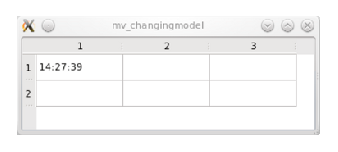
\includegraphics[width=0.5\textwidth]{clock}
\end{figure}

我们仍然使用一个只读表,但是这次内容每秒更改一次,因为我们正在显示当前时间。

(文件:examples/widgets/tutorials/modelview/3\_changingmodel/mymodel.cpp)

\begin{lstlisting}{language=C++}
QVariant MyModel::data(const QModelIndex &index, int role) const
{
    int row = index.row();
    int col = index.column();

    if (role == Qt::DisplayRole && row == 0 && col == 0)
        return QTime::currentTime().toString();

    return QVariant();
}
\end{lstlisting}

缺少一些东西来使时钟滴答作响。我们需要每秒告诉视图时间已更改,并且需要再次读取。
我们用一个计时器来做到这一点。
在构造函数中,我们将其间隔设置为1秒,然后连接其超时信号。

(文件:examples/widgets/tutorials/modelview/3\_changingmodel/mymodel.cpp)

\begin{lstlisting}{language=C++}
MyModel::MyModel(QObject *parent)
    : QAbstractTableModel(parent)
    , timer(new QTimer(this))
{
    timer->setInterval(1000);
    connect(timer, &QTimer::timeout , this, &MyModel::timerHit);
    timer->start();
}
\end{lstlisting}

(文件:examples/widgets/tutorials/modelview/3\_changingmodel/mymodel.cpp)

槽函数:

\begin{lstlisting}{language=C++}
void MyModel::timerHit()
{
    //we identify the top left cell
    QModelIndex topLeft = createIndex(0,0);
    //emit a signal to make the view reread identified data
    emit dataChanged(topLeft, topLeft, {Qt::DisplayRole});
}
\end{lstlisting}

我们通过发射 dataChanged() 信号要求视图再次读取左上角单元格中的数据。
请注意,我们没有将 dataChanged 信号显式连接到视图。这在我们调用 setModel 时自动发生。
\include{./chapter/M/MultithreadingTechnologiesInQt}
\chapter{QMainWindow}

QMainWindow 类用于创建主程序窗口。 更多内容...


\begin{tabular}{|r|l|}
	\hline
	属性 & 方法 \\
	\hline
	头文件 & \#include <QMainWindow>\\      
	\hline
	qmake & QT += widgets\\      
	\hline
	继承: &	QWidget\\
	\hline
\end{tabular}

\begin{compactitem}
\item 列出所有成员函数, 包括继承的成员函数
\end{compactitem}

\section{公共成员类型}

\begin{tabular}{|r|m{25em}|}
	\hline
	类型 & 方法 \\
	\hline
    enum &	DockOption \{ AnimatedDocks, AllowNestedDocks, AllowTabbedDocks, ForceTabbedDocks, VerticalTabs, GroupedDragging \} \\ 
    \hline
    flags &	DockOptions \\ 
	\hline
\end{tabular}

\section{属性}

\begin{tabular}{|r|l|}
	\hline
    属性名 &	类型 \\ 
    \hline
    animated 	& bool \\ 
    \hline
    dockNestingEnabled &	bool\\
    \hline
    dockOptions &	DockOptions\\
    \hline
    documentMode 	&bool\\
    \hline
    iconSize  &	QSize\\
    \hline
    tabShape 	&QTabWidget::TabShape\\
    \hline
    toolButtonStyle &	Qt::ToolButtonStyle\\
    \hline
    unifiedTitleAndToolBarOnMac &	bool\\
	\hline
\end{tabular}

\section{公共成员函数}

\begin{longtable}{|r|m{20em}|}
\hline
返回类型  & 	函数名 \\
\hline
 &QMainWindow (QWidget *parent = nullptr, Qt::WindowFlags flags = Qt::WindowFlags()) \\ 
 \hline
virtual  &	$\sim$QMainWindow () \\
\hline
void 	&addDockWidget (Qt::DockWidgetArea area, QDockWidget *dockwidget) \\ 
\hline
void 	&addDockWidget (Qt::DockWidgetArea area, QDockWidget *dockwidget, Qt::Orientation orientation) \\
\hline
void 	&addToolBar (Qt::ToolBarArea area, QToolBar *toolbar) \\ 
\hline
void 	&addToolBar (QToolBar *toolbar) \\ 
\hline
QToolBar *& 	addToolBar (const QString \&title) \\
\hline
void 	&addToolBarBreak (Qt::ToolBarArea area = Qt::TopToolBarArea) \\
\hline
QWidget *& 	centralWidget () const \\ 
\hline
Qt::DockWidgetArea &	corner (Qt::Corner corner) const \\
\hline
virtual QMenu * &	createPopupMenu () \\
\hline
QMainWindow::DockOptions& 	dockOptions () const\\
\hline
Qt::DockWidgetArea 	&dockWidgetArea (QDockWidget *dockwidget) const\\
\hline
bool &	documentMode () const \\
\hline
QSize &	iconSize () const\\
\hline
void 	&insertToolBar (QToolBar *before, QToolBar *toolbar)\\
\hline
void 	&insertToolBarBreak (QToolBar *before)\\
\hline
bool 	&isAnimated () const\\
\hline
bool 	&isDockNestingEnabled () const\\
\hline
QMenuBar *& 	menuBar () const \\ 
\hline
QWidget * &	menuWidget () const \\ 
\hline
void 	&removeDockWidget (QDockWidget *dockwidget)\\ 
\hline
void 	&removeToolBar (QToolBar *toolbar) \\ 
\hline
void 	&removeToolBarBreak (QToolBar *before) \\ 
\hline
void 	&resizeDocks (const QList<QDockWidget *> \&docks, const QList<int> \&sizes, Qt::Orientation orientation) \\ 
\hline
bool 	&restoreDockWidget (QDockWidget *dockwidget) \\ 
\hline
bool 	&restoreState (const QByteArray \&state, int version = 0) \\ 
\hline
QByteArray &	saveState (int version = 0) const \\ 
\hline
void &	setCentralWidget (QWidget *widget) \\ 
\hline
void &	setCorner (Qt::Corner corner, Qt::DockWidgetArea area) \\ 
\hline
void 	&setDockOptions (QMainWindow::DockOptions options) \\ 
\hline
void &	setDocumentMode (bool enabled) \\ 
\hline
void &	setIconSize (const QSize \&iconSize) \\ 
\hline
void &	setMenuBar (QMenuBar *menuBar) \\ 
\hline
void& 	setMenuWidget (QWidget *menuBar) \\ 
\hline
void &	setStatusBar (QStatusBar *statusbar) \\ 
\hline
void &	setTabPosition (Qt::DockWidgetAreas areas, QTabWidget::TabPosition tabPosition) \\ 
\hline
void &	setTabShape (QTabWidget::TabShape tabShape) \\ 
\hline
void 	&setToolButtonStyle (Qt::ToolButtonStyle toolButtonStyle) \\ 
\hline
void 	&splitDockWidget (QDockWidget *first, QDockWidget *second, Qt::Orientation orientation) \\ 
\hline
QStatusBar * & 	statusBar () const \\ 
\hline
QTabWidget::TabPosition &	tabPosition (Qt::DockWidgetArea area) const \\ 
\hline
QTabWidget::TabShape & 	tabShape () const \\
\hline
QList<QDockWidget *> 	&tabifiedDockWidgets (QDockWidget *dockwidget) const \\
\hline
void &	tabifyDockWidget (QDockWidget *first, QDockWidget *second) \\ 
\hline
QWidget *& 	takeCentralWidget () \\ 
\hline
Qt::ToolBarArea &	toolBarArea (QToolBar *toolbar) const \\ 
\hline
bool &	toolBarBreak (QToolBar *toolbar) const \\ 
\hline
Qt::ToolButtonStyle & 	toolButtonStyle () const \\ 
\hline
bool &	unifiedTitleAndToolBarOnMac () const \\
\hline
\end{longtable}

\section{公共槽}

\begin{tabular}{|r|l|}
\hline
返回类型 &	函数名 \\
\hline
void 	&setAnimated (bool enabled) \\ 
\hline
void 	&setDockNestingEnabled (bool enabled) \\
\hline
void 	&setUnifiedTitleAndToolBarOnMac (bool set) \\
\hline
\end{tabular}

\section{信号}

\begin{tabular}{|r|l|}
    \hline
    返回类型 &	函数名 \\
    \hline
    void &	iconSizeChanged (const QSize \&iconSize) \\ 
    \hline
    void &	tabifiedDockWidgetActivated (QDockWidget *dockWidget) \\ 
    \hline
    void &	toolButtonStyleChanged (Qt::ToolButtonStyle toolButtonStyle) \\
    \hline
\end{tabular}

\section{保护成员函数}

\begin{tabular}{|r|l|}
\hline
返回类型 &	函数名 \\
\hline
virtual void &	contextMenuEvent (QContextMenuEvent *event) override \\
\hline
virtual bool &	event (QEvent *event) override \\
\hline
\end{tabular}

\section{详细描述}
\subsection{Qt 主窗口框架}

主窗口提供了一套创建应用程序用户界面的框架。 Qt 用QMainWindow和 相关类 来管理主窗口。QMainWindow已经定义了一个布局,可以往里添加一些 QToolBar 和 QDockWidget,也可以添加一个 QMenuBar 和一个 QStatusBar。这个布局有一个中央区域,可以放任意部件。如下图所示:

main window layout

\begin{notice}
主窗口必须设置中央部件。
\end{notice}

\subsection{创建主窗口组件}

中央部件通常是标准 Qt 部件,如 QTextEdit 或 QGraphicsView,也可自定义部件。
用setCentralWidget()来设置中央部件。

主窗口可以是单文档界面或多文档界面。 
Qt 中设置 QMdiArea 为中央部件即创建了多文档界面。

下面举例说明主窗口可以添加的部件。

\subsubsection{创建菜单}

Qt 用 QMenu 类实现菜单,主窗口将其放在 QMenuBar。
可以添加 QAction 到QMenu,一个QAction代表菜单中的一个条目。

用menuBar()可以得到主窗口的菜单栏,用 QMenuBar::addMenu 添加菜单。

QMainWindow 默认有一个菜单栏,可以用setMenuBar()自定义一个新的菜单栏。
如果不想用 QMenuBar ,也可以用setMenuWidget()来定制菜单栏。

创建菜单代码示例:

\begin{lstlisting}{language=C++}
void MainWindow::createMenus()
{
    fileMenu = menuBar()->addMenu(tr("&File"));
    fileMenu->addAction(newAct);
    fileMenu->addAction(openAct);
    fileMenu->addAction(saveAct);
}
\end{lstlisting}

createPopupMenu()可以创建弹出式菜单,它会在主窗口收到 context menu 事件时弹出。
停靠部件和菜单栏默认实现了右键菜单,可以重写createPopupMenu()创建自定义菜单。

\subsubsection{创建工具栏}

Qt 用 QToolBar 类实现工具栏,可以用addToolBar()添加工具栏到主窗口。

可以设置 Qt::ToolBarArea 来控制工具栏的初始位置。可以用addToolBarBreak()或insertToolBarBreak()分割工具栏所在的区域,前者可使接下来添加的工具栏换至新的一行,后者添加了一个工具栏分隔符。用 QToolBar::setAllowedAreas 加 QToolBar::setMovable 可以限制用户放工具栏的位置。

工具栏图标的尺寸可以用iconSize()获取,它是平台相关的。可以用setIconSize()设置固定尺寸。用setToolButtonStyle()可以修改工具栏图标外观。

创建工具栏代码示例:

\begin{lstlisting}{language=C++}
void MainWindow::createToolBars()
{
    fileToolBar = addToolBar(tr("File"));
    fileToolBar->addAction(newAct);
}
\end{lstlisting}

\subsection{创建停靠部件}

Qt 用 QDockWidget 类实现停靠部件。停靠部件即可以停靠在主窗口的窗口,可以用 \hl{addDockWidget()} 添加停靠部件到主窗口。

可以设置 \hl{Qt::DockWidgetArea} 来控制停靠部件的位置,有上、下、左、右四种。\hl{setCorner()} 可以让一个角落属于某个相邻的区域。
默认情况下,一个区域只有一个停靠部件,用 \hl{setDockNestingEnabled()} 可以使其能上下或者左右排列多个停靠部件。

两个停靠部件也可以堆叠在一起,然后使用 QTabBar 来选择应显示哪个部件。

创建并添加停靠部件到主窗口的代码示例:


\begin{lstlisting}[language=C++]
QDockWidget *dockWidget = new QDockWidget(tr("Dock Widget"), this);
dockWidget->setAllowedAreas(Qt::LeftDockWidgetArea | Qt::RightDockWidgetArea);
dockWidget->setWidget(dockWidgetContents);
addDockWidget(Qt::LeftDockWidgetArea, dockWidget);
\end{lstlisting}

\subsection{状态栏}

用 \hl{setStatusBar()} 可以设置状态栏,调用 \hl{statusBar()} 会返回主窗口的状态栏。查看 QStatusBar 获取更多内容。

\subsection{存储状态}

QMainWindow 用 \hl{saveState()} 保存布局,用 \hl{restoreState()} 恢复布局。包括工具栏和停靠部件的位置和相对主窗口的尺寸。

\begin{notice}[另请参阅]
QMenuBar,QToolBar,QStatusBar, QDockWidget,Application Example,
Dock Widgets Example,MDI Example,SDI Example 和 Menus Example。
\end{notice}

\section{成员变量文档}

enum QMainWindow::DockOption flags QMainWindow::DockOptions

该枚举包含指定 QMainWindow 停靠行为的标志。

\begin{tabular}{|l|l|m{25em}|}
\hline
函数	& 值	&描述 \\ 
\hline
QMainWindow::AnimatedDocks&	0x01	&同 animated 属性 \\
\hline
QMainWindow::AllowNestedDocks	&0x02&	同 dockNestingEnabled 属性 \\ 
\hline
QMainWindow::AllowTabbedDocks	&0x04	&允许形成下方有 tabBar 的重合部件 \\ 
\hline
QMainWindow::ForceTabbedDocks	&0x08&	每个停靠区域都只包含一个选项卡式停靠部件。
换句话说,停靠区域里不能上下或左右排列停靠部件。如果设置了此选项,则 AllowNestedDocks 不起作用。 \\
\hline
QMainWindow::VerticalTabs	&0x10	&设置 tabBar 在竖直左方位置(默认在下方),包含了 AllowTabbedDocks。另请参阅 setTabPosition () \\ 
\hline
QMainWindow::GroupedDragging	&0x20	&拖动停靠部件的标题栏时,将拖动所有和它在一起的停靠部件。
包含了 AllowTabbedDocks 。在某些停靠部件有区域限制时会有问题。(该枚举值在 Qt 5.6 添加) \\ 
\hline
\end{tabular}

这些选项只是控制停靠部件将如何放入 QMainWindow,不会重新排列停靠部件。
所以要先给停靠部件设置这些选项,再添加到主窗口。AnimatedDocks 和 VerticalTabs 选项例外,它们可以随后设置。

此枚举值在 Qt 4.3 引入和修改

DockOptions 是 QFlags<DockOption> 的 typedef。
它存储 DockOption 值的 OR 组合。

\section{属性文档}

animated : bool

此属性表示是否对操作停靠部件和工具栏进行动画处理

当停靠部件或工具栏在主窗口拖动时,主窗口会显示它们将停靠在什么位置。设置此属性使 QMainWindow 在平滑动画中移动其内容。清除此属性会使它们啪地进入新位置。

默认情况,此属性是生效的。如果主窗口调整尺寸或重绘太慢,可能会无效。

设置此属性与使用 setDockOptions () 设置 AnimatedDocks 选项相同。

该属性在 Qt 4.2 引入

存取函数:

\begin{tabular}{|c|c|}
\hline
    返回类型 &	函数名 \\ 
\hline
bool	& isAnimated() const \\ 
\hline
void	& setAnimated(bool enabled) \\ 
\hline
\end{tabular}

\splitLine

dockNestingEnabled : bool

此属性表示停靠部件是否可以嵌套。

如果此属性为false,停靠区域只能是水平的或垂直的一行。
如果此属性为true,停靠区域所占的区域可以沿任意方向拆分以包含更多的停靠部件。

\begin{quote}
译者注:如果设为 true,两个 dock 可以上面一块,
下面一块,显示在一个区域里,如果设为 false,
则两个 dock 只能变成选项卡式占用一个区域。
\end{quote}

只有在包含大量停靠部件的应用程序中,才需要停靠嵌套。
它给用户更大的自由来组织主窗口。但是,当停靠部件拖过主窗口时,停靠嵌套会导致更加复杂和不太直观的行为。

设置此属性与使用 setDockOptions () 设置 AllowNestedDocks 选项相同。

该属性在 Qt 4.2 引入

存取函数:

\begin{tabular}{|c|c|}
    \hline
    返回类型 &	函数名 \\ 
    \hline
    bool	& isDockNestingEnabled() const \\ 
    \hline
    void	& setDockNestingEnabled(bool enabled) \\ 
    \hline
    \end{tabular}

\splitLine

dockOptions : DockOptions

此属性表示 QMainWindow 的停靠行为

默认值是 AnimatedDocks | AllowTabbedDocks

该属性在 Qt 4.3 引入

存取函数:

\begin{tabular}{|c|c|}
    \hline
    返回类型 &	函数名 \\ 
    \hline
    QMainWindow::DockOptions &	dockOptions() const \\ 
    \hline
    void	&setDockOptions(QMainWindow::DockOptions options) \\ 
    \hline
    \end{tabular}

\splitLine

documentMode : bool

此属性决定选项卡式停靠部件的选项卡栏是否为文档模式。

默认为 false

该属性在 Qt 4.5 引入

存取函数:

\begin{tabular}{|c|c|}
    \hline
    返回类型 &	函数名 \\ 
    \hline
    bool&	documentMode() const \\ 
    \hline
    void&	setDocumentMode(bool enabled) \\ 
    \hline
    \end{tabular}

\begin{notice}[另请参阅]
QTabBar::documentMode
\end{notice}

\splitLine

iconSize : QSize

主窗口工具栏图标的尺寸。

默认是 GUI 样式的默认工具栏图标大小。

\begin{notice}
使用的图标必须至少具有此大小,因为图标只会缩小。
\end{notice}

存取函数:

\begin{tabular}{|c|c|}
    \hline
    返回类型 &	函数名 \\ 
    \hline 
    QSize	&iconSize() const \\ 
    \hline
    void&	setIconSize(const QSize \&iconSize) \\
    \hline
    \end{tabular}

\splitLine

tabShape : QTabWidget::TabShape

此属性表示选项卡式停靠部件的选项卡形状。

默认是 QTabWidget::Rounded

该属性在 Qt 4.5 引入

存取函数:

\begin{tabular}{|c|c|}
    \hline
    返回类型 &	函数名 \\ 
    \hline  
    QTabWidget::TabShape &	tabShape() const \\ 
    \hline
    void 	& setTabShape(QTabWidget::TabShape tabShape) \\ 
    \hline
    \end{tabular}


\begin{notice}[另请参阅]
setTabPosition ()
\end{notice}

\splitLine

toolButtonStyle : Qt::ToolButtonStyle

主窗口的工具栏按钮样式。

若要使工具按钮的样式遵循系统设置,请将此属性设置为 Qt::ToolButtonFollowStyle。
在 Unix 上,将使用桌面环境变量中的用户设置。在其他平台上,Qt::ToolButtonFollowStyle 意思是仅显示图标。

默认是 Qt::ToolButtonIconOnly

存取函数:

\begin{tabular}{|c|c|}
    \hline
    返回类型 &	函数名 \\ 
    \hline  
    Qt::ToolButtonStyle &	toolButtonStyle() const \\ 
    \hline
    void 	& setToolButtonStyle(Qt::ToolButtonStyle toolButtonStyle) \\ 
    \hline
    \end{tabular}

\splitLine

unifiedTitleAndToolBarOnMac : bool

此属性表示窗口是否使用 macOS 上的统一标题和工具栏外观

请注意,与 Qt 4 相比,Qt 5 实现有几个限制:

\begin{compactitem}
\item 不支持在包含 OpenGL 内容的窗口中使用。这包括 QGLWidget 和 QOpenGLWidget。
\item 使用可停靠或可移动工具栏可能会导致绘制错误,不建议使用。
\end{compactitem}

该属性在 Qt 5.2 引入

存取函数:

\begin{tabular}{|c|c|}
    \hline
    返回类型 &	函数名 \\ 
    \hline  
    bool  &	unifiedTitleAndToolBarOnMac() const \\ 
    \hline
    void  &	setUnifiedTitleAndToolBarOnMac(bool set) \\ 
    \hline
    \end{tabular}

\section{成员函数文档}


QMainWindow::QMainWindow(QWidget *parent = nullptr, Qt::WindowFlags flags = Qt::WindowFlags())

主窗口构造函数,指定 parent 和 flags

主窗口设置了 Qt::Window 标志,因此它总作为顶层窗口被创建。

\splitLine

[signal]void QMainWindow::iconSizeChanged(const QSize \&iconSize)

当窗口图标被改变时,将发出此信号。新图标的尺寸为 iconSize。

您可以将此信号连接到其他组件,以帮助保持应用程序的一致外观。

\begin{notice}[另请参阅]
setIconSize ().
\end{notice}

\splitLine

[signal]void QMainWindow::tabifiedDockWidgetActivated(QDockWidget *dockWidget)

当通过选择选项卡激活停靠部件时,将发出此信号。 dockWidget 表示激活的停靠部件。

该函数在 Qt 5.8 引入

\begin{notice}[另请参阅]
tabifyDockWidget() and tabifiedDockWidgets()
\end{notice}

\splitLine

[signal]void QMainWindow::toolButtonStyleChanged(Qt::ToolButtonStyle toolButtonStyle)

当窗口的工具栏按钮样式更改时,将发出此信号。toolButtonStyle 表示新样式。

您可以将此信号连接到其他组件,以帮助保持应用程序的一致外观。

\begin{notice}[另请参阅]
setToolButtonStyle ()
\end{notice}

\splitLine

[virtual]QMainWindow::$\sim$QMainWindow()

销毁主窗口

\splitLine

void QMainWindow::addDockWidget(Qt::DockWidgetArea area, 
    QDockWidget *dockwidget)

添加指定 dockwidget 到指定 area.

\splitLine

void QMainWindow::addDockWidget(Qt::DockWidgetArea area, QDockWidget *dockwidget, Qt::Orientation orientation)

将 dockwidget 添加到指定的 area,方向由 orientation 指定。

\splitLine

void QMainWindow::addToolBar(Qt::ToolBarArea area, QToolBar *toolbar)

在主窗口中将 toolbar 添加到指定的 area。toolbar 放置在当前工具栏块(比如分隔符)的后面。如果主窗口已管理 toolbar,则只会将工具栏移动到 area。


\begin{notice}[另请参阅]
insertToolBar (),addToolBarBreak () 和 insertToolBarBreak ()
\end{notice}

\splitLine

void QMainWindow::addToolBar(QToolBar *toolbar)

这是一个重载函数。

相当于调用 addToolBar(Qt::TopToolBarArea, toolbar)

\splitLine

QToolBar *QMainWindow::addToolBar(const QString \&title)

这是一个重载函数。

创建 QToolBar 的一个对象,设置它的窗口标题为 title 并将它添加到上方的工具栏区域。

\begin{notice}[另请参阅]
setWindowTitle ()
\end{notice}

\splitLine

void QMainWindow::addToolBarBreak(Qt::ToolBarArea area = Qt::TopToolBarArea)

添加一个工具栏 break。这时,新添加的工具条将不再紧跟前一个工具条,而是另起一行。

\splitLine

QWidget *QMainWindow::centralWidget() const

返回主窗口的中央部件。如果尚未设置中央部件,则此函数返回零。

\begin{notice}[另请参阅]
setCentralWidget ()
\end{notice}

\splitLine

[override virtual protected]void QMainWindow::contextMenuEvent(QContextMenuEvent \emph{*event})

重写:QWidget::contextMenuEvent (QContextMenuEvent *event)

Qt::DockWidgetArea QMainWindow::corner(Qt::Corner corner) const

返回占用指定 corner 的停靠部件区域。

\begin{notice}[另请参阅]
setCorner ()
\end{notice}

\splitLine

[virtual]QMenu *QMainWindow::createPopupMenu()

返回一个弹出式菜单,其中包含主窗口中存在的工具栏和停靠部件的可选中条目。如果没有工具栏和停靠小部件,则此函数将返回nullptr。

默认情况下,当用户激活上下文菜单时,主窗口会调用此函数,通常通过右键单击工具栏或停靠部件。

如果要创建自定义弹出式菜单,请重新实现此功能并返回新创建的弹出式菜单。
弹出式菜单的所有权将传输到调用方。

\begin{notice}[另请参阅]
addDockWidget (),addToolBar () 和 menuBar ()
    \end{notice}
    
\splitLine

Qt::DockWidgetArea QMainWindow::dockWidgetArea(QDockWidget \emph{*dockwidget}) const

返回 dockwidget 的 Qt::DockWidgetArea。如果 dockwidget 没有被加入主窗口,此函数返回Qt::NoDockWidgetArea

\begin{notice}[另请参阅]
addDockWidget (),splitDockWidget () 和 Qt::DockWidgetArea
\end{notice}

\splitLine

[override virtual protected]bool QMainWindow::event(QEvent \emph{*event})

重写:QWidget::event (QEvent *event)

\splitLine

void QMainWindow::insertToolBar(QToolBar \emph{*before}, QToolBar \emph{*toolbar})

将 toolbar 插入到 before 工具栏占用的区域之前。
例如,在正常的从左到右布局操作中,toolbar 将显示在水平工具栏区域中 before 工具栏的左侧。

\begin{notice}[另请参阅]
insertToolBarBreak (),addToolBar () 和 addToolBarBreak ()
\end{notice}

\splitLine

void QMainWindow::insertToolBarBreak(QToolBar \emph{*before})

在 before 工具栏左侧插入一个工具栏 break。

\splitLine

QMenuBar *QMainWindow::menuBar() const

返回主窗口的菜单栏。如果菜单栏不存在,则此函数将创建并返回一个空菜单栏。

如果希望 Mac 应用程序中的所有窗口共享一个菜单栏,请不要使用此函数来创建它,
因为此处创建的菜单栏将把 QMainWindow 作为它的父对象。
必须创建一个没有父对象的菜单栏,然后可以在所有 Mac 窗口之间共享该菜单栏。

这样创建:

\begin{lstlisting}{language=C++}
QMenuBar *menuBar = new QMenuBar(nullptr);
\end{lstlisting}

\begin{notice}[另请参阅]
setMenuBar()
\end{notice}

\splitLine

QWidget *QMainWindow::menuWidget() const

返回主窗口的菜单栏。如果尚未构造菜单栏,返回 null。

该函数在 Qt 4.2 引入

\begin{notice}[另请参阅]
setMenuWidget ()
\end{notice}

\splitLine

void QMainWindow::removeDockWidget(QDockWidget \emph{*dockwidget})

从主窗口布局中移除 dockwidget 并将其隐藏。注意,dockwidget 没有被 delete。

\splitLine

void QMainWindow::removeToolBar(QToolBar \emph{*toolbar})

从主窗口布局中移除 toolbar 并将其隐藏。注意,toolbar 没有被 delete。

\splitLine

void QMainWindow::removeToolBarBreak(QToolBar \emph{*before})

删除 before 工具栏之前的一个工具栏 break。

\splitLine

void QMainWindow::resizeDocks(const QList<QDockWidget *> \emph{\&docks},
 const QList<int> \emph{\&sizes}, Qt::Orientation \emph{orientation})

将 \emph{docks} 列表中的停靠部件调整为 \emph{sizes} 列表中的相应尺寸(以像素为单位)。如果 orientation 为 Qt::Horizontal,则调整宽度,否则调整高度。尺寸会调整,以遵守设置的最大尺寸和最小尺寸,并且 QMainWindow 本身不会调整大小。任何多余或缺少的空间将根据尺寸的相对权重分布在部件之间。

示例:

\begin{lstlisting}[language=C++]
resizeDocks({blueWidget, yellowWidget}, {20 , 40}, Qt::Horizontal);
\end{lstlisting}


如果蓝色和黄色部件嵌套在同一级别上,它们将被调整大小,使黄色部件是蓝色部件的两倍大

如果某些部件在选项卡中分组,则每个组只应指定一个部件。不在列表中的部件可能会改变以遵守约束。

该函数在 Qt 5.6 引入

\splitLine

bool QMainWindow::restoreDockWidget(QDockWidget \emph{*dockwidget})

如果在调用 restoreState () 后创建 \emph{dockwidget} 的状态,则恢复状态。
如果状态已恢复,则返回true;否则返回false。

\begin{notice}[另请参阅]
restoreState() 和 saveState()
\end{notice}

\splitLine

bool QMainWindow::restoreState(const QByteArray \emph{\&state}, int version = 0)

还原主窗口工具栏和停靠部件的 \emph{state}。也恢复 corner 的设置。
version 编号与存储在 state 中的号码进行比较。
如果它们不匹配,主窗口的状态保持不变,并且函数将返回false;否则,状态将恢复,函数返回 true。

若要恢复用 QSettings 保存的窗口 geometry,可以这么写:

\begin{lstlisting}{language=C++}
void MainWindow::readSettings()
{
    QSettings settings("MyCompany", "MyApp");
    restoreGeometry(settings.value("myWidget/geometry").toByteArray());
    restoreState(settings.value("myWidget/windowState").toByteArray());
}
\end{lstlisting}

\begin{notice}[另请参阅]
saveState(),QWidget::saveGeometry(),QWidget::restoreGeometry() 和 restoreDockWidget()
\end{notice}

\splitLine

QByteArray QMainWindow::saveState(int version = 0) const

保存主窗口工具栏和停靠部件的当前状态。这包括用 setCorner() 设置的角落区域。
version 作为数据的一部分存储。

objectName 属性用于标识每个 QToolBar 和 QDockWidget。

您应该确保此属性对于添加到 QMainWindow 的每个 QToolBar 和 QDockWidget 是唯一的。

要还原保存的状态,请传递返回值和 version 给 restoreState()。

若要在窗口关闭时保存 geometry,可以这样实现关闭事件:

\begin{lstlisting}{language=C++}
void MyMainWindow::closeEvent(QCloseEvent *event)
{
    QSettings settings("MyCompany", "MyApp");
    settings.setValue("geometry", saveGeometry());
    settings.setValue("windowState", saveState());
    QMainWindow::closeEvent(event);
}
\end{lstlisting}

\begin{notice}[另请参阅]
restoreState(), QWidget::saveGeometry() 和 QWidget::restoreGeometry()
\end{notice}

\splitLine

void QMainWindow::setCentralWidget(QWidget \emph{*widget})

将主窗口的中央部件设置为 \emph{widget}。

\begin{notice}
QMainWindow 拥有 widget 指针的所有权,会在适当的时间将其删除。
\end{notice}

\begin{notice}[另请参阅]
centralWidget()
\end{notice}

\splitLine

void QMainWindow::setCorner(Qt::Corner \emph{corner}, Qt::DockWidgetArea \emph{area})

用停靠部件 area 占据指定的 corner。

\begin{notice}[另请参阅]
corner()
 \end{notice}

\splitLine

void QMainWindow::setMenuBar(QMenuBar \emph{*menuBar})

将主窗口的菜单栏设置为 menuBar。

\begin{notice}
QMainWindow 拥有 menuBar 指针的所有权,会在适当的时间将其删除。\end{notice}

\begin{notice}[另请参阅]
menuBar()
\end{notice}

\splitLine

void QMainWindow::setMenuWidget(QWidget \emph{*menuBar})

将主窗口的菜单栏设置为 \emph{menuBar}。

QMainWindow 拥有 \emph{menuBar} 指针的所有权,会在适当的时间将其删除。

该函数在 Qt 4.2 引入

\begin{notice}[另请参阅]
menuWidget()
\end{notice}

\splitLine

void QMainWindow::setStatusBar(QStatusBar \emph{*statusbar})

将主窗口的状态栏设置为 statusbar。

将状态栏设置为nullptr会将其从主窗口中删除。请注意,QMainWindow 拥有 statusbar 指针的所有权,会在适当的时间将其删除。

\begin{notice}[另请参阅]
statusBar()
\end{notice}

\splitLine

void QMainWindow::setTabPosition(Qt::DockWidgetAreas \emph{areas}, QTabWidget::TabPosition \emph{tabPosition})

将停靠部件 areas 的选项卡位置设置为指定的 tabPosition。默认情况下,所有停靠区域在底部显示其选项卡。

\begin{notice}
VerticalTabs 会覆盖此方法设置的选项卡位置
\end{notice}

该函数在 Qt 4.5 引入

\begin{notice}[另请参阅]
tabPosition() 和 setTabShape()
\end{notice}

\splitLine

void QMainWindow::splitDockWidget(QDockWidget \emph{*first}, QDockWidget \emph{*second}, Qt::Orientation \emph{orientation})

分割停靠部件 first 为两个停靠部件,第一个部件指针传给 first,第二个部件指针传给 second。

orientation 指定了空间的划分。Qt::Horizontal 左右分割;

Qt::Vertical 上下分割。

\begin{notice}
如果 first 位于选项卡式停靠区域中,则 second 将添加为新选项卡,这是因为单个选项卡只能包含一个停靠部件。
    \end{notice}

\begin{notice}
Qt::LayoutDirection 会影响两个分割区域的停靠部件顺序。启用从右到左布局方向时,将反转停靠部件的位置。
\end{notice}


\begin{notice}[另请参阅]
tabifyDockWidget(), addDockWidget() 和 removeDockWidget()
\end{notice}

\splitLine

QStatusBar *QMainWindow::statusBar() const

返回主窗口的状态栏。如果状态栏不存在,则此函数将创建并返回一个空状态栏。

\begin{notice}[另请参阅]
setStatusBar()
\end{notice}

\splitLine

QTabWidget::TabPosition QMainWindow::tabPosition(Qt::DockWidgetArea \emph{area}) const

返回停靠区域 area 的位置。

\begin{notice}
如果设置了 VerticalTabs ,会覆盖此函数的返回值。
\end{notice}

该函数在 Qt 4.5 引入

\begin{notice}[另请参阅]
setTabPosition() 和 tabShape()
\end{notice}

\splitLine

QList<QDockWidget *> QMainWindow::tabifiedDockWidgets(QDockWidget \emph{*dockwidget}) const

返回 \emph{dockwidget} 内堆叠着的停靠部件。

该函数在 Qt 4.5 引入

\begin{notice}[另请参阅]
tabifyDockWidget ()
\end{notice}

\splitLine

void QMainWindow::tabifyDockWidget(QDockWidget \emph{*first}, QDockWidget \emph{*second})

将 \emph{second} 停靠部件移动到 \emph{first} 停靠部件旁形成一个选项卡式停靠区域。

\begin{notice}[另请参阅]
tabifiedDockWidgets()
\end{notice}

\splitLine

QWidget *QMainWindow::takeCentralWidget()

从主窗口中移除中央部件。

返回中央部件的指针。

该函数在 Qt 5.2 引入

\splitLine

Qt::ToolBarArea QMainWindow::toolBarArea(QToolBar \emph{*toolbar}) const

返回 toolbar 的 Qt::ToolBarArea。
 如果主窗口没有添加 toolbar ,返回 Qt::NoToolBarArea。

\begin{notice}[另请参阅]
addToolBar(), addToolBarBreak() 和 Qt::ToolBarArea
\end{notice}

\splitLine

bool QMainWindow::toolBarBreak(QToolBar \emph{*toolbar}) const

返回 \emph{toolbar} 之前是否有工具栏 break。

\begin{notice}[另请参阅]
addToolBarBreak() 和 insertToolBarBreak()
    \end{notice}
\chapter{QMap}

template <typename Key, typename T> class QMap

QMap 类是一种模板类,提供基于红黑树的字典类结构。更多内容...


\begin{tabular}{|r|l|}
	\hline
	属性 & 方法 \\
	\hline
	头文件 & \#include <QMap>\\      
	\hline
	qmake & QT += core\\      
	\hline
	派生类:	& QMultiMap \\
	\hline
\end{tabular}

\begin{compactitem}
\item 所有成员列表,包括继承的成员
\item 废弃的成员
\end{compactitem}

\begin{notice}
该类中的所有函数都是可重入的。
\end{notice}

\section{公共成员类型}

\begin{longtable}{|r|l|}
\hline
class	& const\_iterator \\
\hline
class &	iterator \\ 
\hline
class &	key\_iterator \\ 
\hline
typedef	&ConstIterator \\ 
\hline
typedef	&Iterator \\ 
\hline
typedef	&const\_key\_value\_iterator \\
\hline
typedef	&difference\_type \\        
\hline
typedef	&key\_type \\
\hline
typedef & key\_value\_iterator \\
\hline
typedef	&mapped\_type \\ 
\hline
typedef	&size\_type \\ 
\hline
\end{longtable}

\section{公共成员函数}

\begin{longtable}{|r|m{22em}|}
\hline
& QMap(const typename std::map<Key, T> \&other) \\
\hline
&QMap(QMap<Key, T> \&\&other)\\
\hline
& QMap(const QMap<Key, T> \&other)\\
\hline
& QMap(std::initializer\_list<std::pair<Key, T>> list)\\
\hline
& Map()\\
\hline
QMap<Key, T> &	operator=(QMap<Key, T> \&\&other) \\
\hline 
QMap<Key, T> &	operator=(const QMap<Key, T> \&other)\\ 
\hline
& $\sim$QMap() \\
\hline
QMap::iterator &	begin() \\ 
\hline
QMap::const\_iterator	&begin() const \\
\hline
QMap::const\_iterator&	cbegin() const \\
\hline
QMap::const\_iterator &	cend() const \\ 
\hline
void	& clear() \\ 
\hline
QMap::const\_iterator &	constBegin() const \\ 
\hline
QMap::const\_iterator &	constEnd() const \\
\hline
QMap::const\_iterator&	constFind(const Key \&key) const \\
\hline
QMap::const\_key\_value\_iterator&	constKeyValueBegin() const \\
\hline
QMap::const\_key\_value\_iterator&	constKeyValueEnd() const \\
\hline
bool &	contains(const Key \&key) const \\
\hline
int	&count(const Key \&key) const \\
\hline
int	&count() const \\ 
\hline
bool&	empty() const \\
\hline
QMap::iterator	& end() \\
\hline
QMap::const\_iterator	& end() const \\ 
\hline
QPair<QMap::iterator, QMap::iterator> &	equal\_range(const Key \&key) \\    
\hline
QPair<QMap::const\_iterator, QMap::const\_iterator> &	equal\_range(const Key \&key) const \\
\hline 
QMap::iterator	&erase(QMap::iterator pos) \\ 
\hline
QMap::iterator	&find(const Key \&key) \\
\hline
QMap::const\_iterator	&find(const Key \&key) const \\ 
\hline
T &	first() \\ 
\hline
const T &	first() const \\
\hline
const Key &	firstKey() const \\
\hline
QMap::iterator	&insert(const Key \&key, const T \&value) \\
\hline
QMap::iterator	&insert(QMap::const\_iterator pos, const Key \&key, const T \&value) \\
\hline
void	&insert(const QMap<Key, T> \&map)\\
\hline
bool	&isEmpty() const \\
\hline
const Key & key(const T \&value, const Key \&defaultKey = Key()) const \\
\hline
QMap::key\_iterator&	keyBegin() const\\
\hline
QMap::key\_iterator &	keyEnd() const \\
\hline
QMap::key\_value\_iterator	&keyValueBegin() \\
\hline
QMap::const\_key\_value\_iterator&	keyValueBegin() const \\
\hline
QMap::key\_value\_iterator&	keyValueEnd() \\ 
\hline
QMap::const\_key\_value\_iterator&	keyValueEnd() const \\
\hline
QList&	keys() const \\
\hline
QList	&keys(const T \&value) const \\
\hline
T &	last() \\ 
\hline
const T &	last() const \\ 
\hline
const Key &	lastKey() const \\ 
\hline
QMap::iterator	&lowerBound(const Key \&key) \\ 
\hline
QMap::const\_iterator	&lowerBound(const Key \&key) const \\
\hline
int	&remove(const Key \&key) \\
\hline
int &	size() const \\ 
\hline
void & swap(QMap<Key, T> \&other) \\ 
\hline
T	& take(const Key \&key) \\ 
\hline
std::map<Key, T> &	toStdMap() const \\
\hline
QMap::iterator&	upperBound(const Key \&key) \\ 
\hline
QMap::const\_iterator &	upperBound(const Key \&key) const \\
\hline
const T	& value(const Key \&key, const T \&defaultValue = T()) const \\
\hline
QList	& values() const\\ 
\hline
bool	& operator!=(const QMap<Key, T> \&other) const \\ 
\hline
bool	& operator==(const QMap<Key, T> \&other) const \\ 
\hline
T &	operator[](const Key \&key) \\ 
\hline
const T	 &operator[](const Key \&key) const \\ 
\hline
\end{longtable}

\section{相关非成员函数}

\begin{longtable}{|r|l|}
\hline
返回类型  & 	函数名 \\
\hline
QDataStream &	operator<<(QDataStream \&out, const QMap<Key, T> \&map) \\ 
\hline
QDataStream &	operator>>(QDataStream \&in, QMap<Key, T> \&map) \\  
\hline
\end{longtable}

\section{详细描述}

QMap<Key, T> 是一种 Qt 泛型容器类。
该类存储键值对,可以用相关联的键快速查找值。

QMap 的功能与 QHash 非常相似。二者的区别在于:

\begin{compactitem}
\item QHash 的平均查找速度比 QMap 快。(详情请看算法复杂度。)
\item 遍历 QHash 时,元素的顺序是任意的。而遍历 QMap 时,元素总是按照键的顺序排好序的。
\item QHash 的键类型必须提供 operator==() 运算符和全局的 qHash(Key) 函数。QMap 的键类型必须提供 operator<() 运算符来确定全序。从 Qt5.8.1 起,即使底层的 operator<() 运算符没有提供全序,使用指针作为键类型也是安全的。
\end{compactitem}

下面是一个键类型为 QString,值类型为 int 的 QMap 的示例:

\begin{lstlisting}[language=C++]
QMap<QString, int> map;
\end{lstlisting}

可以使用 operator[]() 运算符将键值对插入到 map 中:

\begin{lstlisting}[language=C++]
map["one"] = 1;
map["three"] = 3;
map["seven"] = 7;
\end{lstlisting}


上面的代码将3个键值对插入到 QMap 中:("one", 1),("three", 3) 和 ("seven", 7)。另外一种向 map 中插入元素的方法是使用 insert():

\begin{lstlisting}[language=C++]
map.insert("twelve", 12);
\end{lstlisting}

使用 operator[]() 运算符或 value() 查找值:

\begin{lstlisting}[language=C++]
int num1 = map["thirteen"];
int num2 = map.value("thirteen");
\end{lstlisting}

如果 map 中不存在指定的键,这些函数返回默认构造的值。

如果想检查 map 中是否包含特定键,使用 contains():

\begin{lstlisting}[language=C++]
int timeout = 30;
if (map.contains("TIMEOUT"))
    timeout = map.value("TIMEOUT");
\end{lstlisting}

还有一个 value() 的重载函数,如果 map 中不存在指定键的元素,该函数使用第2个参数作为默认值:


一般推荐使用 contains() 和 value() 而不是 operator[]() 运算符查找 map 中的键。原因是如果 map 中不存在相同键的元素,operator[]() 运算符会默默地将一个元素插入到 map 中(除非 map 是 const 的)。例如,下面的代码片段将在内存中创建1000个元素:

\begin{lstlisting}[language=C++]
// 错误
QMap<int, QWidget *> map;
...
for (int i = 0; i < 1000; ++i) {
    if (map[i] == okButton)
        cout << "Found button at index " << i << Qt::endl;
}
\end{lstlisting}

为了避免这个问题,将上面代码中的 map[i] 替换为 map.value(i)。

如果想遍历 QMap 中存储的所有键值对,可以使用迭代器。
QMap 同时提供 Java 风格迭代器(QMapIterator 和 QMutableMapIterator)和 STL 风格迭代器(QMap::const\_iterator 和 QMap::iterator)。
下面是使用 Java 风格迭代器遍历 QMap<QString, int> 的方法:

\begin{lstlisting}[language=C++]
QMapIterator<QString, int> i(map);
while (i.hasNext()) {
    i.next();
    cout << i.key() << ": " << i.value() << Qt::endl;
}
\end{lstlisting}

下面是相同的代码,不过这次使用 STL 风格迭代器:

\begin{lstlisting}[language=C++]
QMap<QString, int>::const_iterator i = map.constBegin();
while (i != map.constEnd()) {
    cout << i.key() << ": " << i.value() << Qt::endl;
    ++i;
}
\end{lstlisting}

上面的代码按照键的升序遍历各元素。

通常,QMap 每个键只允许有一个值。如果用已经存在的键调用 insert(),先前的值将被删除。例如:

\begin{lstlisting}[language=C++]
map.insert("plenty", 100);
map.insert("plenty", 2000);
// map.value("plenty") == 2000
\end{lstlisting}

然而,可以使用派生类 QMultiMap 在一个键中存储多个值。使用 values(const Key \&key) 取得单个键关联的所有值,该函数返回一个 QList<T>:

\begin{lstlisting}[language=C++]
QList<int> values = map.values("plenty");
for (int i = 0; i < values.size(); ++i)
    cout << values.at(i) << Qt::endl;
\end{lstlisting}

共享同一键的多个元素按照从最新到最早插入的顺序返回。
另外一种方法是调用 find() 取得 STL 风格迭代器,该迭代器指向共享同一键的多个元素中的第一个元素,
然后从该元素开始遍历:

\begin{lstlisting}[language=C++]
QMap<QString, int>::iterator i = map.find("plenty");
while (i != map.end() && i.key() == "plenty") {
    cout << i.value() << Qt::endl;
    ++i;
}
\end{lstlisting}

如果只想从 map 中获取值(而不是键),也可以使用 foreach:

\begin{lstlisting}[language=C++]
QMap<QString, int> map;
...
foreach (int value, map)
    cout << value << Qt::endl;
\end{lstlisting}

移除元素有几种方法。一种是调用 remove();
该函数移除指定键的所有元素。
另一种方法是使用 QMutableMapIterator::remove()。
另外,还可以使用 clear() 清除整个 map。

QMap 键和值的数据类型必须是可赋值数据类型。
这涵盖了大多数可能会遇到的数据类型,但是编译器不会存储 QWidget 这样的对象作为值,应该存储 QWidget *。
另外,QMap 的键类型必须提供 operator<() 运算符。
QMap 用它来保持元素有序,并假定两个键 x 和 y 在 x < y 和 y < x 都不为 true 的情况下相等。

例子:

\begin{lstlisting}[language=C++]
#ifndef EMPLOYEE_H
#define EMPLOYEE_H

class Employee
{
public:
    Employee() {}
    Employee(const QString &name, QDate dateOfBirth);
    ...

private:
    QString myName;
    QDate myDateOfBirth;
};

inline bool operator<(const Employee &e1, const Employee &e2)
{
    if (e1.name() != e2.name())
        return e1.name() < e2.name();
    return e1.dateOfBirth() < e2.dateOfBirth();
}

#endif // EMPLOYEE_H
\end{lstlisting}

该例中,先比较雇员名。如果雇员名相等,再比较二者的生日来分出大小。

\begin{seeAlso}
QMapIterator,QMutableMapIterator,QHash 和 QSet。
\end{seeAlso}

\section{成员类型文档}

typedef QMap::ConstIterator

QMap<Key, T>::const\_iterator 的 Qt 风格的别名。

\splitLine

typedef QMap::Iterator

QMap<Key, T>::iterator 的 Qt 风格的别名。

\splitLine

typedef QMap::const\_key\_value\_iterator

QMap::const\_key\_value\_iterator 类型定义为 QMap 和 QMultiMap 提供 STL 风格迭代器。

除了 operator *() 运算符返回的是键值对而不是值之外,QMap::const\_key\_value\_iterator 基本和 QMap::const\_iterator 相同。

Qt 5.10 中引入该类型定义。

\begin{seeAlso}
QKeyValueIterator。
\end{seeAlso}

\splitLine

typedef QMap::difference\_type

ptrdiff\_t 的类型别名。为兼容 STL 提供。

typedef QMap::key\_type

Key 的类型别名。为兼容 STL 提供。

\splitLine

typedef QMap::key\_value\_iterator
QMap::key\_value\_iterator 类型定义为 QMap 和 QMultiMap 提供 STL 风格迭代器。

除了 operator *() 运算符返回的是键值对而不是值之外,QMap::key\_value\_iterator 基本和 QMap::iterator 相同。

Qt 5.10 中引入该类型定义。

\begin{seeAlso}
QKeyValueIterator。
\end{seeAlso}

\splitLine

typedef QMap::mapped\_type

T 的类型别名。为兼容 STL 提供。

\splitLine

typedef QMap::size\_type

int 的类型别名。为兼容 STL 提供。

\section{成员函数文档}

QMap::QMap(const typename std::map<Key, T> \emph{\&other})

构造一个 \emph{other} 的副本。

\begin{seeAlso}
toStdMap()。
\end{seeAlso}

\splitLine

QMap::QMap(QMap<Key, T> \emph{\&\&other})

移动构造一个 QMap 实例,使该实例指向 \emph{other} 所指向的同一对象。

Qt 5.2 中引入该函数。

\splitLine

QMap::QMap(const QMap<Key, T> \&other)

构造一个 other 的副本。

该操作需要常数时间,因为 QMap 是隐式共享的。这使得从一个函数返回 QMap 非常快。如果共享实例被修改了,它将以线性时间被复制一份(写时拷贝)。

\begin{seeAlso}
operator=()。
\end{seeAlso}

\splitLine

QMap::QMap(std::initializer\_list<std::pair<Key, T>> list)

用初始化列表 list 中每个元素的副本构造一个 map。

只有当程序在 C++11 模式下编译时,该函数才可用。

Qt 5.1 中引入该函数。

\splitLine

QMap::QMap()

构造一个空 map。
 
\begin{seeAlso}
clear()。
\end{seeAlso}
	
\splitLine

QMap<Key, T> \&QMap::operator=(QMap<Key, T> \emph{\&\&other})

移动赋值 \emph{other} 到该 QMap 实例。

Qt 5.2 中引入该函数。

\splitLine

QMap<Key, T> \&QMap::operator=(const QMap<Key, T> \emph{\&other})

将 \emph{other} 赋值给该 map 并返回该 map 的引用。

QMap::$\sim$QMap()

析构 map。该 map 中值的引用及所有该 map 的迭代器都将失效。

\splitLine

QMap::iterator QMap::begin()

返回 STL 风格迭代器,指向 map 中的第一个元素。

\begin{seeAlso}
constBegin() 和 end()。
\end{seeAlso}

\splitLine

QMap::const\_iterator QMap::begin() const

这是一个重载函数。

\splitLine

QMap::const\_iterator QMap::cbegin() const

返回常量类型的 STL 风格迭代器,指向 map 中的第一个元素。

Qt 5.0 中引入该函数。

\begin{seeAlso}
begin() 和 cend()。
\end{seeAlso}

\splitLine

QMap::const\_iterator QMap::cend() const

返回常量类型的 STL 风格迭代器,指向 map 中最后一个元素之后的假想元素。

Qt 5.0 中引入该函数。

\begin{seeAlso}
cbegin() 和 end()。
\end{seeAlso}

\splitLine

void QMap::clear()

从 map 中移除所有元素。

\begin{seeAlso}
remove()。
\end{seeAlso}

\splitLine

QMap::const\_iterator QMap::constBegin() const

返回常量类型的 STL 风格迭代器,指向 map 中的第一个元素。

\begin{seeAlso}
begin() 和 constEnd()。
\end{seeAlso}

\splitLine

QMap::const\_iterator QMap::constEnd() const

返回常量类型的 STL 风格迭代器,指向 map 中最后一个元素之后的假想元素。

\begin{seeAlso}
constBegin() 和 end()。
\end{seeAlso}

\splitLine

QMap::const\_iterator QMap::constFind(const Key \emph{\&key}) const

返回常量类型的迭代器,指向 map 中键为 key 的元素。

如果 map 不包含键为 key 的元素,该函数返回 constEnd()。

Qt 4.1 中引入该函数。

\begin{seeAlso}
find() 和 QMultiMap::constFind()。
\end{seeAlso}

\splitLine

QMap::const\_key\_value\_iterator QMap::constKeyValueBegin() const

返回常量类型的 STL 风格迭代器,指向 map 中的第一项.

Qt 5.10 中引入该函数。

\begin{seeAlso}
keyValueBegin()。
\end{seeAlso}

\splitLine

QMap::const\_key\_value\_iterator QMap::constKeyValueEnd() const

返回常量类型的 STL 风格迭代器,指向 map 中最后一项之后的假想项。

Qt 5.10 中引入该函数。

\begin{seeAlso}
constKeyValueBegin()。
\end{seeAlso}

\splitLine

bool QMap::contains(const Key \emph{\&key}) const

如果该 map 包含键为 \emph{key} 的元素,返回 true;否则返回 false。

\begin{seeAlso}
count() 和 QMultiMap::contains()。
\end{seeAlso}

\splitLine

int QMap::count(const Key \emph{\&key}) const

返回与键 \emph{key} 相关联的元素个数。

\begin{seeAlso}
contains() 和 QMultiMap::count()。
\end{seeAlso}

\splitLine

int QMap::count() const

这是一个重载函数。

同 size().

\splitLine

bool QMap::empty() const

该函数为兼容 STL 提供。与 isEmpty() 等价,
如果 map 为空,返回 true;否则返回 false。

\splitLine

QMap::iterator QMap::end()

返回 STL 风格迭代器,指向 map 中最后一个元素之后的假想元素。

\begin{seeAlso}
begin() 和 constEnd()。
\end{seeAlso}

\splitLine

QMap::const\_iterator QMap::end() const

这是一个重载函数。

\splitLine

QPair<QMap::iterator, QMap::iterator> QMap::equal\_range(const Key \emph{\&key})

返回一对迭代器界定与 key 相关联的值的范围 [first, second)。

\splitLine

QPair<QMap::const\_iterator, QMap::const\_iterator> QMap::equal\_range(const Key \&key) const

这是一个重载函数。

Qt 5.6 中引入该函数。

\splitLine

QMap::iterator QMap::erase(QMap::iterator \emph{pos})

从 map 中移除迭代器 \emph{pos} 指向的键值对,返回指向 map 中下一个元素的迭代器。


\begin{seeAlso}
remove()。
\end{seeAlso}

\splitLine

QMap::iterator QMap::find(const Key \emph{\&key})

返回迭代器,指向 map 中键为 key 的元素。

如果 map 不包含键为 key 的元素,函数返回 end()。

如果 map 包含多个键为 key 的元素,函数返回指向最新插入的那个值的迭代器。
其它值可以通过递增迭代器取得。

例如,下面的代码遍历同一键的所有元素:

\begin{lstlisting}[language=C++]
QMap<QString, int> map;
...
QMap<QString, int>::const_iterator i = map.find("HDR");
while (i != map.end() && i.key() == "HDR") {
    cout << i.value() << Qt::endl;
    ++i;
}
\end{lstlisting}

\begin{seeAlso}
constFind(),value(),values(),lowerBound(),upperBound() 和 QMultiMap::find()。
\end{seeAlso}

\splitLine

QMap::const\_iterator QMap::find(const Key \&key) const

这是一个重载函数。

\splitLine

T \&QMap::first()

返回指向 map 中第一个值的引用,即映射到最小键的值。该函数假定 map 不为空。

对于非共享 map(或者调用的是常量版本),该函数在常数时间内完成。

Qt 5.2 中引入该函数。


\begin{seeAlso}
last(),firstKey() 和 isEmpty()。
\end{seeAlso}

\splitLine

const T \&QMap::first() const

这是一个重载函数。

Qt 5.2 中引入该函数。

\splitLine

const Key \&QMap::firstKey() const

返回 map 中最小键的引用。该函数假定 map 不为空。

该操作在常数时间内完成。

Qt 5.2 中引入该函数。


\begin{seeAlso}
lastKey(),first(),keyBegin() 和 isEmpty()。
\end{seeAlso}

\splitLine

QMap::iterator QMap::insert(const Key \emph{\&key}, const T \emph{\&value})

用键 \emph{key} 和值 \emph{value} 插入一个新元素。

如果已经存在键为 \emph{key} 的元素,该元素的值将被 \emph{value} 替换。

如果有多个键为 \emph{key} 的元素,最新插入的元素的值将被 \emph{value} 替换。

\begin{seeAlso}
QMultiMap::insert()。
\end{seeAlso}

\splitLine

QMap::iterator QMap::insert(QMap::const\_iterator \emph{pos}, const Key \emph{\&key}, const T \emph{\&value})

这是一个重载函数。

用键 key 和值 value 插入一个新元素,pos 用来提示插入位置。

如果以 constBegin() 作为插入位置提示,表明 key 比 map 中的任何键都小,
而 constEnd() 则建议 key(严格)大于 map 中的任何键。
否则提示应该满足条件 (pos - 1).key() < key <= pos.key()。
如果提示 pos 是错误的,其将被忽略,并以常规方式插入。

如果已经存在键为 key 的元素,该元素的值将被 value 替换。

如果有多个键为 key 的元素,只会有一个元素的值被 value 替换。

如果提示是正确的,并且 map 未被共享,插入操作平均在常数时间内完成。

从有序数据创建 map 时,从最大键的元素开始以 constBegin() 作为提示插入,
比按从小到大的顺序以 constEnd() 作为提示插入更快,因为 constEnd() - 1 (用来检查提示是否合法)需要对数时间。

\begin{notice}
需小心对待提示。提供从旧的共享实例取得的迭代器可能引起崩溃,还会有默默污染 map 和 pos 的 map 的风险。
\end{notice}

Qt 5.1 中引入该函数。

\begin{seeAlso}
QMultiMap::insert()。
\end{seeAlso}

\splitLine

void QMap::insert(const QMap<Key, T> \emph{\&map})

将 map 中的所有元素插入到本 \emph{map} 中。

如果一个键同时在两个 \emph{map} 中出现,其值将被传入的 \emph{map} 中存储的值替换。

\begin{seeAlso}
如果传入的 map 中同一键关联多个元素,则该键的最终值未定义。
\end{seeAlso}

Qt 5.15 中引入该函数。

\begin{seeAlso}
QMultiMap::insert()。
\end{seeAlso}

\splitLine

bool QMap::isEmpty() const

如果 map 中不包含元素,返回 true;否则返回 false。

\begin{notice}
size()。
\end{notice}

\splitLine

const Key QMap::key(const T \emph{\&value}, const Key \&defaultKey = Key()) const

这是一个重载函数。

返回与值 \emph{value} 对应的第一个键,如果 map 不包含值为 value 的元素,返回 defaultKey。如果没有提供 defaultKey,函数返回默认构造的键。

该函数可能会比较慢(线性时间),因为 QMap 的内部数据结构是以快速查找键而不是值为目标来优化的。

Qt 4.3 中引入该函数。

\begin{seeAlso}
value() 和 keys()。
\end{seeAlso}

\splitLine

QMap::key\_iterator QMap::keyBegin() const

返回常量类型的 STL 风格迭代器,指向 map 中的第一个键。

Qt 5.6 中引入该函数。

\begin{seeAlso}
keyEnd() 和 firstKey()。
\end{seeAlso}

\splitLine

QMap::key\_iterator QMap::keyEnd() const

返回常量类型的 STL 风格迭代器,指向 map 中的最后一个元素之后的假想元素的键。

Qt 5.6 中引入该函数。

\begin{seeAlso}
keyBegin() 和 lastKey()。
\end{seeAlso}

\splitLine

QMap::key\_value\_iterator QMap::keyValueBegin()

返回 STL 风格迭代器,指向 map 中的第一项。

Qt 5.10 中引入该函数。

\begin{seeAlso}
keyValueEnd().
\end{seeAlso}

\splitLine

QMap::const\_key\_value\_iterator QMap::keyValueBegin() const

返回常量类型的 STL 风格迭代器,指向 map 中的第一项。

Qt 5.10 中引入该函数。

\begin{seeAlso}
keyValueEnd()。
\end{seeAlso}

\splitLine

QMap::key\_value\_iterator QMap::keyValueEnd()

返回 STL 风格迭代器,指向 map 中最后一项之后的假想项。

Qt 5.10 中引入该函数。

\begin{seeAlso}
keyValueBegin()。
\end{seeAlso}

\splitLine

QMap::const\_key\_value\_iterator QMap::keyValueEnd() const

返回常量类型的 STL 风格迭代器,指向 map 中最后一项之后的假想项。

Qt 5.10 中引入该函数。

\begin{seeAlso}
keyValueBegin()。
\end{seeAlso}

\splitLine

QList<Key> QMap::keys() const

以升序返回 map 中所有键的列表。在 map 中多次出现的键(当该方法应用在 QMultiMap 时)也会在列表中多次出现。

键的顺序将确保与通过 values() 返回的值的顺序相同。

\begin{seeAlso}
QMultiMap::uniqueKeys(),values() 和 key()。
\end{seeAlso}

\splitLine

QList<Key> QMap::keys(const T \emph{\&value}) const

这是一个重载函数。

以升序返回所有与值 \emph{value} 相关联的键的列表。

该函数可能会比较慢(线性时间),因为 QMap 的内部数据结构是以快速查找键而不是值为目标来优化的。

\splitLine

T \&QMap::last()

返回 map 中最后一个值的引用,即映射到最大键的值。该函数假定 map 不为空。

对于非共享 map(或者调用的是常量版本),该函数在对数时间内完成。

Qt 5.2 中引入该函数。

\begin{seeAlso}
first(),lastKey() 和 isEmpty()。
\end{seeAlso}

\splitLine

const T \&QMap::last() const

这是一个重载函数。

Qt 5.2 中引入该函数。

\splitLine

const Key \&QMap::lastKey() const

返回 map 中最大键的引用。该函数假定 map 不为空。

该函数在对数时间内完成。

Qt 5.2 中引入该函数。

\begin{seeAlso}
firstKey(),last(),keyEnd() 和 isEmpty()。
\end{seeAlso}

\splitLine

QMap::iterator QMap::lowerBound(const Key \emph{\&key})

返回指向 map 中键 \emph{key} 所关联的第一个元素的迭代器。如果 map 不包含键为 key 的元素,函数返回指向距离下一个键最近的元素的迭代器。

例子:

\begin{lstlisting}[language=C++]
QMap<int, QString> map;
map.insert(1, "one");
map.insert(5, "five");
map.insert(10, "ten");

map.lowerBound(0);      // 返回指向 (1, "one") 的迭代器
map.lowerBound(1);      // 返回指向 (1, "one") 的迭代器
map.lowerBound(2);      // 返回指向 (5, "five") 的迭代器
map.lowerBound(10);     // 返回指向 (10, "ten") 的迭代器
map.lowerBound(999);    // 返回 end()
\end{lstlisting}

如果 map 包含多个键为 key 的元素,该函数返回指向最新插入的值的迭代器。其它值可以通过递增迭代器访问。例如,下面的例子遍历同一键所关联的所有元素:

\begin{lstlisting}[language=C++]
QMap<QString, int> map;
...
QMap<QString, int>::const_iterator i = map.lowerBound("HDR");
QMap<QString, int>::const_iterator upperBound = map.upperBound("HDR");
while (i != upperBound) {
    cout << i.value() << Qt::endl;
    ++i;
}
\end{lstlisting}

%%%%%%%%%
\begin{seeAlso}
upperBound() 和 find()。
\end{seeAlso}
    

QMap::const\_iterator QMap::lowerBound(const Key \emph{\&key}) const

这是一个重载函数。

\splitLine

int QMap::remove(const Key \emph{\&key})

从 map 中移除所有键为 \emph{key} 的元素。返回被移除的元素个数,如果键存在,则为1,否则为0。

\begin{seeAlso}
clear(),take() 和 QMultiMap::remove()。
\end{seeAlso}

\splitLine

int QMap::size() const

返回 map 中键值对的个数。

\begin{seeAlso}
isEmpty() 和 count()。
\end{seeAlso}
    

\splitLine

void QMap::swap(QMap<Key, T> \emph{\&other})

将 map other 与本 map 交换。该操作非常快,永远不失败。

Qt 4.8 中引入该函数。

\splitLine

T QMap::take(const Key \emph{\&key})

从 map 中移除键为 \emph{key} 的元素,返回键 \emph{key} 所关联的值。

如果 map 中不存在该元素,该函数简单返回一个默认构造的值。如果 map 中有多个键为 key 的元素,只移除最新插入的元素并返回值。

如果不使用返回值,使用 remove() 更高效一些。

\begin{seeAlso}
remove()。
\end{seeAlso}

\splitLine

std::map<Key, T> QMap::toStdMap() const

返回与这个 QMap 相对应的 STL map。

\splitLine

QMap::iterator QMap::upperBound(const Key \emph{\&key})

返回迭代器,指向 map 中首个大于键 \emph{key} 的元素。如果 map 不包含键为 \emph{key} 的元素,该函数返回指向距离下一个键最近的元素的迭代器。

例子:

\begin{lstlisting}[language=C++]
QMap<int, QString> map;
map.insert(1, "one");
map.insert(5, "five");
map.insert(10, "ten");

map.upperBound(0);      // 返回指向 (1, "one") 的迭代器
map.upperBound(1);      // 返回指向 (5, "five") 的迭代器
map.upperBound(2);      // 返回指向 (5, "five") 的迭代器
map.upperBound(10);     // 返回 end()
map.upperBound(999);    // 返回 end()
\end{lstlisting}

%%%%%%
\begin{seeAlso}
lowerBound() 和 find()。
\end{seeAlso}

QMap::const\_iterator QMap::upperBound(const Key \emph{\&key}) const

这是一个重载函数。

\splitLine

const T QMap::value(const Key \emph{\&key}, const T \&defaultValue = T()) const

返回键 key 关联的值。

如果 map 不包含键为 \emph{key} 的元素,该函数返回 defaultValue。 如果没有指定 defaultValue,该函数返回默认构造的值。如果 map 中有多个键为 key 的元素,返回最新插入的元素的值。

\begin{seeAlso}
key(),values(),contains() 和 operator[]()。
\end{seeAlso}

\splitLine

QList<T> QMap::values() const

按照键升序返回 map 中所有值的列表。如果一个键关联到多个值,该键的所有值都将被放入列表中,而不只是最新插入的值。

\begin{seeAlso}
keys() 和 value()。
\end{seeAlso}

\splitLine

bool QMap::operator!=(const QMap<Key, T> \emph{\&other}) const

如果 other 与本 map 不相等,返回 true,否则返回 false。

如果两个 map 包含相同的键值对,则认为二者相等。

该函数需要值类型实现 operator==()。

\begin{seeAlso}
operator==()。
\end{seeAlso}

\splitLine

bool QMap::operator==(const QMap<Key, T> \emph{\&other}) const

如果 \emph{other} 与本 map 相等,返回 true,否则返回 false。

如果两个 map 包含相同的键值对,则认为二者相等。

该函数需要值类型实现 operator==()。

\begin{seeAlso}
operator!=()。
\end{seeAlso}

\splitLine

T \&QMap::operator[](const Key \emph{\&key})

返回键 \emph{key} 所关联的值的可修改引用。

如果 map 不包含键为 \emph{key} 的元素,该函数用键 \emph{key} 插入一个默认构造的值,并返回该值的引用。
如果 map 包含多个键为  \emph{key} 的元素,该函数返回最新插入的那个值的引用。

\begin{seeAlso}
insert() 和 value()。
\end{seeAlso}

\splitLine

const T QMap::operator[](const Key \emph{\&key}) const

这是一个重载函数。

同 value()。

\section{相关非成员函数}

template <typename Key, typename T> QDataStream \&operator<<(QDataStream \emph{\&out}, const QMap<Key, T> \emph{\&map})

将 \emph{map} 写出到流 \emph{out}。

该函数需要键和值类型实现 operator<<()。

\begin{seeAlso}
QDataStream 运算符的格式。
\end{seeAlso}

\splitLine

template <typename Key, typename T> QDataStream \&operator>>(QDataStream \emph{\&in}, QMap<Key, T> \emph{\&map})

从流 in 读入数据到 map。

该函数需要键和值类型实现 operator>>()。

\begin{seeAlso}
QDataStream 运算符的格式。
\end{seeAlso}
\chapter{QMapIterator}

template <typename Key, typename T> class QMapIterator

QMapIterator 类为 QMap 和 QMultiMap 提供 Java 风格的常量迭代器。更多内容...

\begin{tabular}{|r|l|}
	\hline
	属性 & 方法 \\
	\hline
	头文件 & \#include <QMapIterator>\\      
	\hline
	qmake & QT += core\\      
	\hline
\end{tabular}

\begin{compactitem}
\item 所有成员列表,包括继承的成员
\end{compactitem}

\section{公共成员函数}

\begin{longtable}{|r|l|}
\hline
& QMapIterator(const QMap<Key, T> \&map) \\ 
\hline
QMapIterator<Key, T> \& 	& operator=(const QMap<Key, T> \&container) \\ 
\hline
bool 	& findNext(const T \&value) \\ 
\hline
bool 	& findPrevious(const T \&value) \\
\hline
bool &	hasNext() const \\
\hline
bool &	hasPrevious() const \\ 
\hline
const Key & 	key() const \\
\hline
QMapIterator::Item &	next() \\ 
\hline
QMapIterator::Item 	&peekNext() const \\ 
\hline
QMapIterator::Item &	peekPrevious() const \\ 
\hline
QMapIterator::Item 	&previous() \\ 
\hline
void 	&toBack() \\
\hline
void 	&toFront() \\ 
\hline
const T \& & 	value() const \\ 
\hline
\end{longtable}

\section{详细描述}

QMap 同时提供 Java 风格迭代器 和 STL 风格迭代器。
Java 风格迭代器比 STL 风格迭代器更高级,更容易使用;
同时也略微低效。

QMapIterator<Key, T> 用来遍历 QMap (或 QMultiMap)。
如果想在遍历时修改 map,要使用 QMutableMapIterator。

QMapIterator 构造函数接受 QMap 作为参数。
构造后,迭代器位于 map 的最开始位置(第一个元素之前)。
下面的例子演示如何顺序遍历所有元素:

\begin{cppcode}
QMap<int, QWidget *> map;
...
QMapIterator<int, QWidget *> i(map);
while (i.hasNext()) {
    i.next();
    qDebug() << i.key() << ": " << i.value();
}
\end{cppcode}

next() 函数返回 map 中的下一个元素并将迭代器前移。
key() 和 value() 函数返回跳过的最后一个元素的键和值。

与 STL 风格迭代器不同,Java 风格迭代器指向元素之间而不是直接指向元素。
第一次调用 next() 前移迭代器到第一个和第二个元素之间的位置,并返回第一个元素;
第二次调用 next() 前移迭代器到第二个和第三个元素之间的位置;以此类推。


\begin{figure}[hpt!]  
	\centering
    \includegraphics[width=0.5\textwidth]{javaiterators1}
\end{figure}

%%%%%%%%

下面的例子演示如何反序遍历元素:

\begin{cppcode}
QMapIterator<int, QWidget *> i(map);
i.toBack();
while (i.hasPrevious()) {
    i.previous();
    qDebug() << i.key() << ": " << i.value();
\end{cppcode}

如果想查找特定值的所有实例,循环使用 findNext() 或 findPrevious()。例如:

\begin{cppcode}
QMapIterator<int, QWidget *> i(map);
while (i.findNext(widget)) {
    qDebug() << "Found widget " << widget << " under key "
             << i.key();
}
\end{cppcode}

同一 map 可以使用多个迭代器。
如果在 QMapIterator 处于活动状态时修改 map,QMapIterator 将继续在原 map 上遍历,
而忽略修改后的副本。

\begin{seeAlso}
QMutableMapIterator 和 QMap::const\_iterator。
\end{seeAlso}

\section{成员函数文档}

bool QMapIterator::findPrevious(const T \emph{\&value})

从当前迭代器位置开始向后查找值 \emph{value}。
如果找到值为 \emph{value} 的键值对,返回 true;
否则返回 false。

调用该函数后,如果找到值,迭代器将被移动到匹配元素的前面;
否则,迭代器将被移动到容器的前端。

\begin{seeAlso}
findNext()。
\end{seeAlso}

\splitLine

bool QMapIterator::findNext(const T \emph{\&value})

从当前迭代器位置开始向前查找值 \emph{value}。
如果找到值为 \emph{value} 的键值对,返回 true;
否则返回 false。

调用该函数后,如果找到值 \emph{value},迭代器将被移动到匹配元素的后面;
否则,迭代器将被移动到容器的末端。

\begin{seeAlso}
findPrevious()。
\end{seeAlso}
    
\splitLine

const Key \&QMapIterator::key() const

调用遍历函数(next(),previous(),findNext(),findPrevious())后,该函数返回跳过的最后一个元素的键。

调用 next() 或 findNext() 后,key() 与 peekPrevious().key() 相同。调用 previous() 或 findPrevious() 后,key() 与 peekNext().key() 相同。

\begin{seeAlso}
value()。
\end{seeAlso}

\splitLine

QMapIterator::Item QMapIterator::peekPrevious() const

不移动迭代器而返回前一个元素。

对返回值调用 key() 获取元素的键,调用 value() 获取元素的值。

对位于容器前端的迭代器调用该函数将导致未定义结果。

\begin{seeAlso}
hasPrevious(),previous() 和 peekNext()。
\end{seeAlso}

\splitLine

QMapIterator::Item QMapIterator::previous()

返回前一个元素并将迭代器向后移动一个位置。

对返回值调用 key() 获取元素的键,调用 value() 获取元素的值。

对位于容器前端的迭代器调用该函数将导致未定义结果。


\begin{seeAlso}
hasPrevious(),peekPrevious() 和 next()。
\end{seeAlso}

\splitLine

bool QMapIterator::hasPrevious() const

如果该迭代器前面至少有一个元素,返回 true,即该迭代器不在容器的前端;否则返回 false。

\begin{seeAlso}
hasNext() 和 previous()。
\end{seeAlso}

\splitLine

bool QMapIterator::hasNext() const

如果该迭代器后面至少有一个元素,返回 true,即该迭代器不在容器的末端;否则返回 false。

\begin{seeAlso}
hasPrevious() 和 next()。
\end{seeAlso}

\splitLine

void QMapIterator::toBack()

将迭代器移动到容器的末端(最后一个元素之后)。

\begin{seeAlso}
toFront() 和 previous()。
\end{seeAlso}

\splitLine

void QMapIterator::toFront()

将迭代器移动到容器的前端(第一个元素之前)。

\begin{seeAlso}
toBack() 和 next()。
\end{seeAlso}

\splitLine

QMapIterator<Key, T> \&QMapIterator::operator=(const QMap<Key, T> \emph{\&container})

将迭代器关联到 \emph{container} 来遍历 map。迭代器将被移动到 map 的前端(第一个元素之前)。


\begin{seeAlso}
toFront() 和 toBack()。
\end{seeAlso}

\splitLine

QMapIterator::QMapIterator(const QMap<Key, T> \emph{\&map})

构造一个迭代器来遍历 \emph{map}。迭代器将被移动到 \emph{map} 的前端(第一个元素之前)。


\begin{seeAlso}
operator=()。
\end{seeAlso}

\splitLine

QMapIterator::Item QMapIterator::next()

返回下一个元素并将迭代器向前移动一个位置。

对返回值调用 key() 获取元素的键,调用 value() 获取元素的值。

对位于容器末端的迭代器调用该函数将导致未定义结果。

\begin{seeAlso}
hasNext(),peekNext() 和 previous()。
\end{seeAlso}
    
\splitLine

QMapIterator::Item QMapIterator::peekNext() const

不移动迭代器而返回下一个元素。

对返回值调用 key() 获取元素的键,调用 value() 获取元素的值。

对位于容器末端的迭代器调用该函数将导致未定义结果。

\begin{seeAlso}
hasNext(),next() 和 peekPrevious()。
\end{seeAlso}

\splitLine

const T \&QMapIterator::value() const

调用遍历函数(next(),previous(),findNext(),findPrevious())后,该函数返回跳过的最后一个元素的值。

调用 next() 或 findNext() 后,value() 与 peekPrevious().value() 相同。

调用 previous() 或 findPrevious() 后,value() 与 peekNext().value() 相同。

\begin{seeAlso}
key()。
\end{seeAlso}
\chapter{QMetaClassInfo}

QMetaClassInfo 类提供了某个类的附加信息。更多内容...

\begin{tabular}{|r|l|}
	\hline
	属性 & 方法 \\
	\hline
	头文件 & \#include <QMetaClassInfo>\\      
	\hline
	qmake & QT += core\\      
	\hline
\end{tabular}

\section{公共成员函数}

\begin{tabular}{|r|l|}   
\hline
const char * 	&name() const \\
\hline
const char * 	& value() const \\ 
\hline
\end{tabular}

\section{详细描述}

类型信息对象指的在源代码中通过 Q\_CLASSINFO() 指定的名称-值对。
这些信息可以通过 name() 和 value() 获取,例如:

\begin{lstlisting}[language=C++]
class MyClass
{
    Q_OBJECT
    Q_CLASSINFO("author", "Sabrina Schweinsteiger")
    Q_CLASSINFO("url", "http://doc.moosesoft.co.uk/1.0/")

public:
    ...
};
\end{lstlisting}

此机制可以在您的应用中自由使用,Qt 不会在自身的任何类中使用它。

\begin{notice}[另请参阅]
QMetaObject。
\end{notice}

\section{成员函数文档}

const char *QMetaClassInfo::name() const

返回本信息对象的名称。

\begin{notice}[另请参阅]
value()。
\end{notice}

const char *QMetaClassInfo::value() const

返回本信息对象的值。

\begin{notice}[另请参阅]
name()。
\end{notice}


\chapter{QMetaMethod}

QMetaMethod 类提供了对应一个成员函数的元数据。更多内容...

\begin{tabular}{|r|l|}
	\hline
	属性 & 方法 \\
	\hline
	头文件 & \#include <QMetaMethod>\\      
	\hline
	qmake & QT += core\\      
	\hline
\end{tabular}

\section{公共类型}

\begin{tabular}{|r|l|}   
\hline
类型	& 名称 \\ 
\hline
enum	&Access \{ Private, Protected, Public \} \\ 
\hline
enum	& MethodType \{ Method, Signal, Slot, Constructor \} \\
\hline
\end{tabular}

\section{公共成员函数}

\begin{longtable}{|l|m{27em}|} 
\hline
返回类型 & 函数 \\   
\hline
QMetaMethod::Access	& access() const \\ 
\hline
bool &	invoke(QObject *object, Qt::ConnectionType connectionType, QGenericReturnArgument returnValue, QGenericArgument val0 = QGenericArgument(nullptr), QGenericArgument val1 = QGenericArgument(), QGenericArgument val2 = QGenericArgument(), QGenericArgument val3 = QGenericArgument(), QGenericArgument val4 = QGenericArgument(), QGenericArgument val5 = QGenericArgument(), QGenericArgument val6 = QGenericArgument(), QGenericArgument val7 = QGenericArgument(), QGenericArgument val8 = QGenericArgument(), QGenericArgument val9 = QGenericArgument()) const \\
\hline
bool &	invoke(QObject *object, QGenericReturnArgument returnValue, QGenericArgument val0 = QGenericArgument(0), QGenericArgument val1 = QGenericArgument(), QGenericArgument val2 = QGenericArgument(), QGenericArgument val3 = QGenericArgument(), QGenericArgument val4 = QGenericArgument(), QGenericArgument val5 = QGenericArgument(), QGenericArgument val6 = QGenericArgument(), QGenericArgument val7 = QGenericArgument(), QGenericArgument val8 = QGenericArgument(), QGenericArgument val9 = QGenericArgument()) const \\
\hline
bool &	invoke(QObject *object, Qt::ConnectionType connectionType, QGenericArgument val0 = QGenericArgument(0), QGenericArgument val1 = QGenericArgument(), QGenericArgument val2 = QGenericArgument(), QGenericArgument val3 = QGenericArgument(), QGenericArgument val4 = QGenericArgument(), QGenericArgument val5 = QGenericArgument(), QGenericArgument val6 = QGenericArgument(), QGenericArgument val7 = QGenericArgument(), QGenericArgument val8 = QGenericArgument(), QGenericArgument val9 = QGenericArgument()) const \\
\hline
bool &	invoke(QObject *object, QGenericArgument val0 = QGenericArgument(0), QGenericArgument val1 = QGenericArgument(), QGenericArgument val2 = QGenericArgument(), QGenericArgument val3 = QGenericArgument(), QGenericArgument val4 = QGenericArgument(), QGenericArgument val5 = QGenericArgument(), QGenericArgument val6 = QGenericArgument(), QGenericArgument val7 = QGenericArgument(), QGenericArgument val8 = QGenericArgument(), QGenericArgument val9 = QGenericArgument()) const \\
\hline
bool &	invokeOnGadget(void *gadget, QGenericReturnArgument returnValue, QGenericArgument val0 = QGenericArgument(nullptr), QGenericArgument val1 = QGenericArgument(), QGenericArgument val2 = QGenericArgument(), QGenericArgument val3 = QGenericArgument(), QGenericArgument val4 = QGenericArgument(), QGenericArgument val5 = QGenericArgument(), QGenericArgument val6 = QGenericArgument(), QGenericArgument val7 = QGenericArgument(), QGenericArgument val8 = QGenericArgument(), QGenericArgument val9 = QGenericArgument()) const \\
\hline
bool &	invokeOnGadget(void *gadget, QGenericArgument val0 = QGenericArgument(0), QGenericArgument val1 = QGenericArgument(), QGenericArgument val2 = QGenericArgument(), QGenericArgument val3 = QGenericArgument(), QGenericArgument val4 = QGenericArgument(), QGenericArgument val5 = QGenericArgument(), QGenericArgument val6 = QGenericArgument(), QGenericArgument val7 = QGenericArgument(), QGenericArgument val8 = QGenericArgument(), QGenericArgument val9 = QGenericArgument()) const \\
\hline
const char * 	&name() const \\
\hline
const char * 	& value() const \\ 
\hline
bool & 	isValid() const \\ 
\hline
int	& methodIndex() const \\ 
\hline
QByteArray &	methodSignature() const \\ 
\hline
QMetaMethod::MethodType	 & methodType() const \\
\hline
QByteArray & 	name() const \\ 
\hline
int	& parameterCount() const \\
\hline
QList<QByteArray>	& parameterNames() const \\
\hline
int	& parameterType(int index) const \\
\hline
QList<QByteArray> &	parameterTypes() const \\
\hline
int	& returnType() const \\
\hline
int	& revision() const \\ 
\hline
const char *	& tag() const \\ 
\hline
const char *	& typeName() const \\ 
\hline
\end{longtable}


\section{静态公共成员}


\begin{tabular}{|l|l|}
\hline
返回类型 &	函数 \\ 
\hline
QMetaMethod 	&fromSignal(PointerToMemberFunction \emph{signal}) \\ 
\hline
\end{tabular}

\section{相关非成员函数}

\begin{tabular}{|l|l|}
\hline
返回类型 &	函数 \\ 
\hline
bool  &	operator!=(const QMetaMethod \emph{\&m1}, const QMetaMethod \emph{\&m2}) \\
\hline 
bool  &	operator==(const QMetaMethod \emph{\&m1}, const QMetaMethod \emph{\&m2})  \\
\hline
\end{tabular}

\section{宏定义}

\begin{tabular}{|c|c|}
	\hline
	宏定义 \\ 
	\hline
Q\_METAMETHOD\_INVOKE\_MAX\_ARGS \\ 
	\hline
	\end{tabular}

\section{详细描述}

QMetaMethod 类具有一个 methodType()、一个 methodSignature()、一组 parameterTypes() 和 parameterNames()、返回值的 typeName()、一个 tag()、一个 access() 描述符。
可以通过 invoke() 来执行任意 QObject 的方法。

\begin{notice}[另请参阅]
QMetaObject、QMetaEnum、QMetaProperty 和 Qt 属性系统。
\end{notice}

\section{成员类型文档}

enum QMetaMethod::Access

此枚举描述某方法的访问权限,遵循 C++ 相关公约。


\begin{tabular}{|c|c|}
	\hline
	常量 	& 数值  \\
	\hline
	QMetaMethod::Private  &	0 \\ 
	\hline
	QMetaMethod::Protected &	1 \\ 
	\hline
	QMetaMethod::Public &	2 \\ 
	\hline
	\end{tabular}

enum QMetaMethod::MethodType	

\begin{tabular}{|c|c|c|}
	\hline
	常量  &	数值 	& 描述  \\ 
	\hline
	QMetaMethod::Method &	0 &	该函数是普通的成员函数。 \\
	\hline
	QMetaMethod::Signal &	1 	&该函数是信号函数。 \\
	\hline
	QMetaMethod::Slot &	2 &	该函数是槽函数。 \\ 
	\hline
	QMetaMethod::Constructor &	3 &	该函数是构造函数。 \\ 
	\hline
	\end{tabular}

\section{成员函数文档}

QMetaMethod::Access QMetaMethod::access() const

返回该方法的访问权限(private、protected 或 `public)。

\begin{notice}
信号永远是公共的,但应将此认为是实现细节。在类外发射该类的信号通常是个坏主意。
\end{notice}

\begin{notice}[另请参阅]
methodType()。
\end{notice}

[static] template <typename PointerToMemberFunction> QMetaMethod QMetaMethod::fromSignal(PointerToMemberFunction signal)

返回对应给定 signal 的元方法,若 signal 并非信号,则返回无效的 QMetaMethod 对象。

范例:

\begin{lstlisting}[language=C++]
QMetaMethod destroyedSignal = QMetaMethod::fromSignal(&QObject::destroyed);
\end{lstlisting}


本函数在 Qt 5.0 中被引入。

bool QMetaMethod::invoke(QObject *object, Qt::ConnectionType connectionType, QGenericReturnArgument returnValue, 
   QGenericArgument val0 = QGenericArgument(nullptr), 
   QGenericArgument val1 = QGenericArgument(), 
QGenericArgument val2 = QGenericArgument(), 
QGenericArgument val3 = QGenericArgument(), 
QGenericArgument val4 = QGenericArgument(), 
QGenericArgument val5 = QGenericArgument(), 
QGenericArgument val6 = QGenericArgument(), 
QGenericArgument val7 = QGenericArgument(),
 QGenericArgument val8 = QGenericArgument(), 
 QGenericArgument val9 = QGenericArgument()) const

通过 object 对象动态调用本方法。若可被动态调用则返回 tue,若该对象无此方法或参数不匹配则返回 false。

该动态调用可以是同步或异步的,由 connectionType 决定:

\begin{compactitem}
\item 若 type 是 Qt::DirectConnection,则该方法会被立即执行。
\item 若 type 是 Qt::QueuedConnection,则会发送一个 QEvent ,该方法会在应用进入该对象所属线程的主事件循环后执行。
\item 若 type 是 Qt::AutoConnection,当 object 与调用者处于相同线程中时,该方法会被同步执行,否则会被异步执行。
\end{compactitem}

返回值会被存放在 returnvalue 中。若调用方式是异步,则返回值无法被获取。
最多可以传递十个参数 (val0, val1, val2, val3, val4, val5, val6, val7, val8 和 val9) 至本方法。

QGenericArgument 和 QGenericReturnArgument 是内部的辅助类。
为了动态调用信号槽,您需要将参数通过 Q\_ARG() 和 Q\_RETURN\_ARG() 宏进行封装。
Q\_ARG() 接受一个类型名称和一个该类型的不可变引用;
Q\_RETURN\_ARG() 接受一个类型名称和一个该类型的可变引用。

通过异步方式动态调用 QPushButton 的 animateClick() 槽:

\begin{lstlisting}[language=C++]
int methodIndex = pushButton->metaObject()->indexOfMethod("animateClick()");
QMetaMethod method = metaObject->method(methodIndex);
method.invoke(pushButton, Qt::QueuedConnection);
\end{lstlisting}

当异步调用方法时,传递的参数必须被 Qt 的元对象系统所知悉,因为 Qt 需要在后台事件中拷贝并保存它们。
如果您使用队列连接时遇到下述错误信息:

\begin{lstlisting}
QMetaMethod::invoke: Unable to handle unregistered datatype 'MyType'	
\end{lstlisting}

则在调用 invokeMethod() 之前通过 qRegisterMetaType() 来注册该数据类型。

若想通过 obj 对象同步调用 \hl{compute(QString, int, double)} 槽,则代码如下:

\begin{lstlisting}[language=C++]
QString retVal;
QByteArray normalizedSignature = QMetaObject::normalizedSignature("compute(QString, int, double)");
int methodIndex = obj->metaObject()->indexOfMethod(normalizedSignature);
QMetaMethod method = obj->metaObject()->method(methodIndex);
method.invoke(obj,
              Qt::DirectConnection,
              Q_RETURN_ARG(QString, retVal),
              Q_ARG(QString, "sqrt"),
              Q_ARG(int, 42),
              Q_ARG(double, 9.7));
\end{lstlisting}


此处使用了 QMetaObject::normalizedSignature() 来确保函数签名符合 invoke() 期望的格式,即将多余的空白移除。

若 compute 槽通过特定顺序没有完整获取到一个 QString、一个 int 和一个 double,则此调用会失败。

\begin{notice}[警告]
此方法不会验证参数的有效性,object 必须是创建 QMetaMethod 的 QMetaObject 的类型实例,参数列表必须与该方法的保持一直,否则会导致未定义行为。
\end{notice}

\begin{notice}[另请参阅]
Q\_ARG()、Q\_RETURN\_ARG()、qRegisterMetaType() 和 QMetaObject::invokeMethod()。
\end{notice}


%%%%%%%%%

bool QMetaMethod::invoke(QObject *object, QGenericReturnArgument returnValue, QGenericArgument val0 = QGenericArgument(0), QGenericArgument val1 = QGenericArgument(), QGenericArgument val2 = QGenericArgument(), QGenericArgument val3 = QGenericArgument(), QGenericArgument val4 = QGenericArgument(), QGenericArgument val5 = QGenericArgument(), QGenericArgument val6 = QGenericArgument(), QGenericArgument val7 = QGenericArgument(), QGenericArgument val8 = QGenericArgument(), QGenericArgument val9 = QGenericArgument()) const

此函数是 invoke() 的重载。

此重载始终通过 Qt::AutoConnection 调用本方法。

bool QMetaMethod::invoke(QObject *object, Qt::ConnectionType connectionType, QGenericArgument val0 = QGenericArgument(0), QGenericArgument val1 = QGenericArgument(), QGenericArgument val2 = QGenericArgument(), QGenericArgument val3 = QGenericArgument(), QGenericArgument val4 = QGenericArgument(), QGenericArgument val5 = QGenericArgument(), QGenericArgument val6 = QGenericArgument(), QGenericArgument val7 = QGenericArgument(), QGenericArgument val8 = QGenericArgument(), QGenericArgument val9 = QGenericArgument()) const

此函数是 invoke() 的重载。

此重载用于不关心对返回值的场合。

bool QMetaMethod::invoke(QObject *object, QGenericArgument val0 = QGenericArgument(0), QGenericArgument val1 = QGenericArgument(), QGenericArgument val2 = QGenericArgument(), QGenericArgument val3 = QGenericArgument(), QGenericArgument val4 = QGenericArgument(), QGenericArgument val5 = QGenericArgument(), QGenericArgument val6 = QGenericArgument(), QGenericArgument val7 = QGenericArgument(), QGenericArgument val8 = QGenericArgument(), QGenericArgument val9 = QGenericArgument()) const

此函数是 invoke() 的重载。

此重载通过 Qt::AutoConnection 调用本方法,并忽略返回值。

bool QMetaMethod::invokeOnGadget(void \emph{*gadget}, QGenericReturnArgument \emph{returnValue}, QGenericArgument \emph{val0} = QGenericArgument(nullptr), QGenericArgument val1 = QGenericArgument(), QGenericArgument val2 = QGenericArgument(), QGenericArgument val3 = QGenericArgument(), QGenericArgument val4 = QGenericArgument(), QGenericArgument val5 = QGenericArgument(), QGenericArgument val6 = QGenericArgument(), QGenericArgument val7 = QGenericArgument(), QGenericArgument val8 = QGenericArgument(), QGenericArgument val9 = QGenericArgument()) const

通过 Q\_GADGET 对象动态调用本方法。
若可被动态调用则返回 tue,若该对象无此方法或参数不匹配则返回 false。

gadget 指针必须是 Q\_GADGET 类的实例。

该调用始终是同步的。

返回值会被存放在 returnvalue 中。若调用方式是异步,则返回值无法被获取。最多可以传递十个参数 (val0, val1, val2, val3, val4, val5, val6, val7, val8 和 val9) 至本方法。

\begin{notice}[另请参阅]
此方法不会验证参数的有效性,gadget 必须是创建 QMetaMethod 的 QMetaObject 的类型实例,参数列表必须与该方法的保持一直,否则会导致未定义行为。
\end{notice}

本函数在 Qt 5.5 中被引入。

\begin{notice}[另请参阅]
Q\_ARG()、Q\_RETURN\_ARG()、qRegisterMetaType() 和 QMetaObject::invokeMethod()。
\end{notice}

bool QMetaMethod::invokeOnGadget(void \*gadget, QGenericArgument val0 = QGenericArgument(0), QGenericArgument val1 = QGenericArgument(), QGenericArgument val2 = QGenericArgument(), QGenericArgument val3 = QGenericArgument(), QGenericArgument val4 = QGenericArgument(), QGenericArgument val5 = QGenericArgument(), QGenericArgument val6 = QGenericArgument(), QGenericArgument val7 = QGenericArgument(), QGenericArgument val8 = QGenericArgument(), QGenericArgument val9 = QGenericArgument()) const

这是一个重载函数。

此重载函数通过 gadget 对象动态调用本方法,并忽略返回值。

本函数在 Qt 5.5 中被引入。

bool QMetaMethod::isValid() const

若此方法有效则返回 true(即可被自省并动态调用),否则返回 false。

本函数在 Qt 5.0 中被引入。

int QMetaMethod::methodIndex() const

返回本方法的索引编号。

本函数在 Qt 4.6 中被引入。

QByteArray QMetaMethod::methodSignature() const

返回本方法的签名(例如 setValue(double))。

本函数在 Qt 5.0 中被引入。

\begin{notice}[另请参阅]
parameterTypes() 和 parameterNames()。
\end{notice}

QMetaMethod::MethodType QMetaMethod::methodType() const

返回本方法的类型(signal、slot、method 或 constructor)。

\begin{notice}[另请参阅]
access()。
\end{notice}

QByteArray QMetaMethod::name() const

返回本方法的名字。

本函数在 Qt 5.0 中被引入。

\begin{notice}[另请参阅]
methodSignature() 和 parameterCount()。
\end{notice}

int QMetaMethod::parameterCount() const

返回本方法的参数个数。

本函数在 Qt 5.0 中被引入。

\begin{notice}[另请参阅]
parameterType() 和 parameterNames()。
\end{notice}

QList<QByteArray> QMetaMethod::parameterNames() const

返回参数名称列表。

\begin{notice}[另请参阅]
parameterTypes() 和 methodSignature()。
\end{notice}

int QMetaMethod::parameterType(int \emph{index}) const

返回对应 index 的参数类型。

返回值是 QMetaType 中注册的类型之一,若该类型未被注册则返回 QMetaType::UnknownType。

本函数在 Qt 5.0 中被引入。

\begin{notice}[另请参阅]
parameterCount()、returnType() 和 QMetaType。
\end{notice}

QList<QByteArray> QMetaMethod::parameterTypes() const

返回参数类型的列表。

\begin{notice}[另请参阅]
parameterNames() 和 methodSignature()。
\end{notice}

int QMetaMethod::returnType() const

返回本方法返回值的类型。

返回

返回值是 QMetaType 中注册的类型之一,若该类型未被注册则返回 QMetaType::UnknownType。

本函数在 Qt 5.0 中被引入。

\begin{notice}[另请参阅]
parameterType()、QMetaType 和 typeName()。
\end{notice}

int QMetaMethod::revision() const

返回通过 Q\_REVISION 注明的版本,若未注明则返回 0。

本函数在 Qt 5.1 中被引入。

const char *QMetaMethod::tag() const

返回与本方法关联的标签。

标签在此处指的是可以被 moc 识别的特定宏,用于为方法添加附加信息。

标签信息可以用如下方式添加到函数声明中:

\begin{lstlisting}[language=C++]
// 在 MainWindow 类声明中
#ifndef Q_MOC_RUN
// 将标签内容定义为空,以确保对编译器不可见
#  define MY_CUSTOM_TAG
#endif
...
private slots:
	MY_CUSTOM_TAG void testFunc();
\end{lstlisting}

相关信息可通过如下方式获取:

\begin{lstlisting}[language=C++]
MainWindow win;
win.show();

int functionIndex = win.metaObject()->indexOfSlot("testFunc()");
QMetaMethod mm = win.metaObject()->method(functionIndex);
qDebug() << mm.tag(); // 将打印 MY_CUSTOM_TAG
\end{lstlisting}

%%%%%%%%

此时,moc 会提取并记录所有标签,但不会对它们做任何特殊处理。您可以用标签来标注不同的方法,并在您的应用中通过特定的用途来使用它们。

\begin{notice}
自 Qt 5.0 开始,moc 会展开预编译宏,所以必须将标签定义包含在 \#ifndef Q\_MOC\_RUN 中,正如上文范例。
这在 Qt 4 中不是必要的,但上述代码在 Qt 4 中同样也能生效。
\end{notice}

const char *QMetaMethod::typeName() const

返回本方法的返回类型名称。

\begin{notice}[另请参阅]
returnType() 和 QMetaType::type()。
\end{notice}

\section{相关非成员函数}

bool operator!=(const QMetaMethod \emph{\&m1}, const QMetaMethod\emph{\&m2})

这是一个重载函数。

若 m1 与 m2 不相等则返回 true,否则返回 false。

本函数在 Qt 5.0 中被引入。

bool operator==(const QMetaMethod \emph{\&m1}, const QMetaMethod \emph{\&m2})

这是一个重载函数。

若 m1 与 m2 相等则返回 true,否则返回 false。

本函数在 Qt 5.0 中被引入。

\section{宏定义文档}

Q\_METAMETHOD\_INVOKE\_MAX\_ARGS

此宏的数值等于通过 QMetaMethod::invoke() 执行方法时,可以传递的最大参数个数。
\chapter{QMetaObject 结构体}

QMetaObject 类包含了 Qt 对象的元信息。更多内容...。

\begin{tabular}{|r|l|}
	\hline
	属性 & 方法 \\
	\hline
	头文件 & \#include <QMetaObject>\\      
	\hline
	qmake & QT += core\\      
	\hline
\end{tabular}

\section{公共成员类型}


\begin{tabular}{|r|l|}   
\hline
类型	& 名称 \\ 
\hline
class	& Connection \\ 
\hline
\end{tabular}


\section{公共成员函数}

\begin{longtable}{|r|m{28em}|}   
\hline
QMetaClassInfo	& classInfo(int \emph{index}) const \\ 
\hline
int &	classInfoCount() const \\
\hline
int	&classInfoOffset() const\\
\hline
const char *	&className() const\\
\hline
QMetaMethod	&constructor(int index) const\\
\hline
int	&constructorCount() const\\
\hline
QMetaEnum	&enumerator(int index) const\\
\hline
int	&enumeratorCount() const\\
\hline
int	&enumeratorOffset() const\\
\hline
int&	indexOfClassInfo(const char *name) const\\
\hline
int	&indexOfConstructor(const char *constructor) const\\
\hline
int	&indexOfEnumerator(const char *name) const\\
\hline
int	&indexOfMethod(const char *method) const\\
\hline
int	&indexOfProperty(const char *name) const\\
\hline
int	&indexOfSignal(const char *signal) const\\
\hline
int&	indexOfSlot(const char *slot) const\\
\hline
bool	&inherits(const QMetaObject *metaObject) const\\
\hline
QMetaMethod	&method(int index) const\\
\hline
int	&methodCount() const\\
\hline
int	&methodOffset() const\\
\hline
QObject *	&newInstance(QGenericArgument val0 = QGenericArgument(nullptr), QGenericArgument val1 = QGenericArgument(), QGenericArgument val2 = QGenericArgument(), QGenericArgument val3 = QGenericArgument(), QGenericArgument val4 = QGenericArgument(), QGenericArgument val5 = QGenericArgument(), QGenericArgument val6 = QGenericArgument(), QGenericArgument val7 = QGenericArgument(), QGenericArgument val8 = QGenericArgument(), QGenericArgument val9 = QGenericArgument()) const\\
\hline
QMetaProperty	&property(int index) const\\
\hline
int&	propertyCount() const\\
\hline
int	&propertyOffset() const\\
\hline
const QMetaObject *	&superClass() const\\
\hline
QMetaProperty	&userProperty() const\\
\hline
\end{longtable}



\section{静态公共成员}

\begin{longtable}{|l|m{28em}|}
\hline
返回类型 &	函数 \\ 
\hline
bool	&checkConnectArgs(const char *signal, const char *method) \\
\hline
bool	&checkConnectArgs(const QMetaMethod \&signal, const QMetaMethod \&method) \\
\hline
void	&connectSlotsByName(QObject *object) \\
\hline
bool	&invokeMethod(QObject *obj, const char *member, Qt::ConnectionType type, QGenericReturnArgument ret, QGenericArgument val0 = QGenericArgument(nullptr), QGenericArgument val1 = QGenericArgument(), QGenericArgument val2 = QGenericArgument(), QGenericArgument val3 = QGenericArgument(), QGenericArgument val4 = QGenericArgument(), QGenericArgument val5 = QGenericArgument(), QGenericArgument val6 = QGenericArgument(), QGenericArgument val7 = QGenericArgument(), QGenericArgument val8 = QGenericArgument(), QGenericArgument val9 = QGenericArgument())\\
\hline
bool	&invokeMethod(QObject *obj, const char *member, QGenericReturnArgument ret, QGenericArgument val0 = QGenericArgument(0), QGenericArgument val1 = QGenericArgument(), QGenericArgument val2 = QGenericArgument(), QGenericArgument val3 = QGenericArgument(), QGenericArgument val4 = QGenericArgument(), QGenericArgument val5 = QGenericArgument(), QGenericArgument val6 = QGenericArgument(), QGenericArgument val7 = QGenericArgument(), QGenericArgument val8 = QGenericArgument(), QGenericArgument val9 = QGenericArgument())\\
\hline
bool	&invokeMethod(QObject *obj, const char *member, Qt::ConnectionType type, QGenericArgument val0 = QGenericArgument(0), QGenericArgument val1 = QGenericArgument(), QGenericArgument val2 = QGenericArgument(), QGenericArgument val3 = QGenericArgument(), QGenericArgument val4 = QGenericArgument(), QGenericArgument val5 = QGenericArgument(), QGenericArgument val6 = QGenericArgument(), QGenericArgument val7 = QGenericArgument(), QGenericArgument val8 = QGenericArgument(), QGenericArgument val9 = QGenericArgument())\\
\hline
bool	&invokeMethod(QObject *obj, const char *member, QGenericArgument val0 = QGenericArgument(0), QGenericArgument val1 = QGenericArgument(), QGenericArgument val2 = QGenericArgument(), QGenericArgument val3 = QGenericArgument(), QGenericArgument val4 = QGenericArgument(), QGenericArgument val5 = QGenericArgument(), QGenericArgument val6 = QGenericArgument(), QGenericArgument val7 = QGenericArgument(), QGenericArgument val8 = QGenericArgument(), QGenericArgument val9 = QGenericArgument())\\
\hline
bool	&invokeMethod(QObject *context, Functor function, Qt::ConnectionType type = Qt::AutoConnection, FunctorReturnType *ret = nullptr) \\
\hline
bool	&invokeMethod(QObject *context, Functor function, FunctorReturnType *ret) \\
\hline
QByteArray&	normalizedSignature(const char *method) \\
\hline
QByteArray&	normalizedType(const char *type)\\
\hline
\end{longtable}

\section{宏定义}

\begin{tabular}{|l|l|}
\hline
返回类型	& 宏定义 \\
\hline
QGenericArgument	& Q\_ARG(Type, const Type \&value) \\
\hline
QGenericReturnArgument&	Q\_RETURN\_ARG(Type, Type \&value) \\
\hline
\end{tabular}



\section{详细描述}

Qt 的元对象系统负责信号槽跨对象通信机制、运行时类型信息和 Qt 的属性系统。
应用中的每个 QObject 子类都有一个唯一的 QMetaObject 实例(译者注:与类一一对应,即同一个 QObject 子类的任意对象,都使用同一个 QMetaObject),其中保存了这个 QObject 子类的所有元信息,可以通过 QObject::metaObject() 获取。

QMetaObject 在应用编写中通常不需要,但在进行元编程时会非常有用,例如脚本引擎或者用户界面生成器。

最常用的成员函数有:

\begin{compactitem}
\item className() 返回类的名称。
\item superClass() 返回父类对应的元对象。
\item method() 和 methodCount() 提供关于一个类的元方法(信号、槽和其它可动态调用的成员方法)。
\item enumerator() 和 enumeratorCount() 提供一个类的枚举类型的信息。
\item propertyCount() 和 property() 提供一个类的属性的信息。
\item constructor() 和 constructorCount() 提供一个类的元构造函数的信息。
\end{compactitem}


索引函数 indexOfConstructor()、indexOfMethod()、indexOfEnumerator() 和 indexOfProperty() 将构造函数、成员函数、枚举类型和属性的名称映射为索引。例如,当连接信号槽时,Qt 内部使用 indexOfMethod() 进行检索。

类可以拥有一系列 名称—数值 格式的附加信息,保存在 QMetaClassInfo 对象中。信息条目数量可通过 classInfoCount()查询, classInfo()返回单条信息,也可通过 indexOfClassInfo() 检索信息条目。

\begin{notice}
元对象系统的操作通常是线程安全的,比如元对象是在编译期生成的静态只读实例。
然而,如果元对象在被程序动态修改了(如通过 QQmlPropertyMap),应用需要显示地同步对相关对象的访问。
\end{notice}

\begin{notice}[另请参阅]
QMetaClassInfo、QMetaEnum、QMetaMethod、QMetaProperty、QMetaType 和 Meta-Object System。
\end{notice}

\section{成员函数文档}

[static] bool QMetaObject::checkConnectArgs(const char \emph{*signal}, const char \emph{*method})

如果 signal 和 method 的参数能够匹配则返回 true,否则返回 false。

signal 和 method 都被假设是已经规范化的。

\begin{notice}[另请参阅]
normalizedSignature()。
\end{notice}

[static] bool QMetaObject::checkConnectArgs(const QMetaMethod \emph{\&signal}, const QMetaMethod \emph{\&method})

这是一个重载函数。

如果 signal 和 method 的参数能够匹配则返回 true,否则返回 false。

本函数在 Qt 5.0 中被引入。

QMetaClassInfo QMetaObject::classInfo(int \emph{index}) const

返回对应 index 的类型信息的元数据对象。

范例:

\begin{lstlisting}[language=C++]
class MyClass : public QObject
 {
     Q_OBJECT
     Q_CLASSINFO("author", "Sabrina Schweinsteiger")
     Q_CLASSINFO("url", "http://doc.moosesoft.co.uk/1.0/")

 public:
     ...
 };
\end{lstlisting}


%%%%%%%%%%%%%%%%

\begin{notice}[另请参阅]
classInfoCount()、classInfoOffset() 和 indexOfClassInfo()。
\end{notice}

int QMetaObject::classInfoCount() const

返回该类信息条目数量。

\begin{notice}[另请参阅]
classInfo()、classInfoOffset() 和 indexOfClassInfo()。
\end{notice}

int QMetaObject::classInfoOffset() const

返回类信息在该类中的偏移量,即第一条类信息的编号。

若该类没有包含类信息的父类,则偏移量为 0,否则偏移量是所有父类的类信息数量的总和。

\begin{notice}[另请参阅]
classInfo()、classInfoCount() 和 indexOfClassInfo()。
\end{notice}

const char *QMetaObject::className() const

返回该类的名称。

\begin{notice}[另请参阅]
superClass()。
\end{notice}

[static] void QMetaObject::connectSlotsByName(QObject \emph{*object})

递归检索 object 和所有子对象,将它们的信号连接至 object 中匹配的槽,匹配格式如下:

\begin{lstlisting}
void on_<对象名>_<信号名>(<信号参数>);
\end{lstlisting}

假设有一个对象名 为 button1 的 QPushButton 类型的子对象,则捕获它的 clicked() 信号的槽应为:

\begin{lstlisting}
void on_button1_clicked();
\end{lstlisting}

若 object 对象自身的名字已设置,则它自己的信号也会被连接至对应的槽。

\begin{notice}[另请参阅]
QObject::setObjectName().
\end{notice}

%%%%%%%%%%%
QMetaMethod QMetaObject::constructor(int \emph{index}) const

返回指定 index 的构造函数的元数据。

该函数在 Qt 4.5 中被引入。

\begin{notice}[另请参阅]
constructorCount() 和 newInstance()。
\end{notice}

int QMetaObject::constructorCount() const

返回此类的构造函数个数。

该函数在 Qt 4.5 中被引入。

\begin{notice}[另请参阅]
constructor() 和 indexOfConstructor()。
\end{notice}

QMetaEnum QMetaObject::enumerator(int \emph{index}) const

返回指定 index 的枚举类型的元数据。

\begin{notice}[另请参阅]
enumeratorCount()、enumeratorOffset() 和 indexOfEnumerator()。
\end{notice}

int QMetaObject::enumeratorCount() const

返回该类的枚举类型的个数。

\begin{notice}[另请参阅]
enumerator()、enumeratorOffset() 和 indexOfEnumerator()。
\end{notice}
	
int QMetaObject::enumeratorOffset() const

返回该类的枚举类型偏移量,即首个枚举变量的编号。

若该类没有包含枚举类型的父类,则偏移量为 0,否则偏移量是所有父类的枚举类型数量的总和。

\begin{notice}[另请参阅]
enumerator()、enumeratorCount() 和 indexOfEnumerator()。
\end{notice}

int QMetaObject::indexOfClassInfo(const char \emph{*name}) const

查找名为 name 的类型信息条目并返回其编号,未找到则返回-1。

\begin{notice}[另请参阅]
classInfo()、classInfoCount() 和 classInfoOffset()。
\end{notice}

int QMetaObject::indexOfConstructor(const char \emph{*constructor}) const

查找名为 constructor 的构造函数并返回其编号,未找到则返回-1。

注意:constructor 需要为规范化的格式,如 normalizedSignature() 的返回值。

该函数在 Qt 4.5 中被引入。

另请参阅:constructor()、constructorCount() 和 normalizedSignature()。

int QMetaObject::indexOfEnumerator(const char *name) const

查找名为 name 的枚举类型并返回其编号,未找到则返回-1。

另请参阅:enumerator(), enumeratorCount() 和 enumeratorOffset().

int QMetaObject::indexOfMethod(const char *method) const

查找名为 method 的方法并返回其编号,未找到则返回-1。

注意:method 需要为规范化的格式,如 normalizedSignature() 的返回值。

另请参阅:method()、methodCount()、methodOffset() 和 normalizedSignature()。

int QMetaObject::indexOfProperty(const char *name) const

查找名为 name 的属性并返回其编号,未找到则返回-1。

\begin{notice}[另请参阅]
property()、propertyCount() 和 propertyOffset()。	
\end{notice}

int QMetaObject::indexOfSignal(const char \emph{*signal}) const

查找名为 name 的信号并返回其编号,未找到则返回-1。

此方法与 indexOfMethod() 相似,区别是若该方法存在但并非信号函数,则会返回 -1。

\begin{notice}
signal 需要为规范化的格式,如 normalizedSignature() 的返回值。	
\end{notice}

\begin{notice}[另请参阅]
indexOfMethod()、normalizedSignature(), method()、methodCount() 和 methodOffset()。
\end{notice}

int QMetaObject::indexOfSlot(const char \emph{*slot}) const

查找名为 name 的槽并返回其编号,未找到则返回-1。

此方法与 indexOfMethod() 相似,区别是若该方法存在但并非槽函数,则会返回 -1。

\begin{notice}[另请参阅]
indexOfMethod()、method()、methodCount() 和 methodOffset()。
\end{notice}


bool QMetaObject::inherits(const QMetaObject \emph{*metaObject}) const

若该 QMetaObject 继承自 metaObject 描述的类型,则返回 true,否则返回 false。

一个类型被认为是继承自它自己的。

该函数在 Qt 5.7 中被引入。
\chapter{Connection}

QMetaObject::Connection 类。

\section{公共成员函数}

\begin{tabular}{|r|l|}
	\hline
返回类型  &	函数 \\ 
\hline
	&Connection(Connection \emph{\&\&o}) \\ 
    \hline
	&Connection(const Connection \emph{\&other}) \\ 
    \hline
	&Connection() \\ 
    \hline
Connection & 	operator=(Connection \emph{\&\&other}) \\ 
\hline
Connection & 	operator=(const Connection \emph{\&other}) \\
	& $\sim$Connection() \\ 
    \hline
bool &	operator bool() const    \\ 
	\hline
\end{tabular}


\section{详细描述}

代表一组信号槽(或信号-仿函数)连接的句柄。

此类可被用于检查连接是否有效,或通过 QObject::disconnect() 断开连接。
对于不具备上下文对象的 信号-仿函数 连接,这是唯一的断开连接的方式。

由于 Connection 仅仅是一个句柄,当被销毁或重新赋值时,底层的信号槽连接不会被影响。

\section{成员函数文档}

Connection::Connection(Connection \emph{\&\&o})

移动构造函数,将其指向 \hl{o} 原先指向的对象。

Connection::Connection(const Connection \emph{\&other})

生成 \hl{other} 连接的句柄的一份拷贝。

Connection::Connection()

创建一个空的连接实例。

Connection \&Connection::operator=(Connection \emph{\&\&other})

将 \hl{other} 转移赋值至本对象,并返回本对象的引用。

Connection \&Connection::operator=(const Connection \emph{\&other})

将 \hl{other} 赋值给本对象,并返回本对象的引用。

Connection::$\sim$Connection()

QMetaObject::Connection 的析构函数。

bool Connection::operator bool() const

若该对象有效,则返回 \hl{true}。

若 QObject::connect 成功,则该连接是有效的;
若 QObject::connect 无法找到对应的信号槽或参数不匹配,则该连接无效。
\chapter{QMetaProperty}

QMetaProperty 类提供了对应一条属性的元数据。更多内容...

\begin{tabular}{|r|l|}
	\hline
	属性 & 方法 \\
	\hline
<<<<<<< HEAD
    头文件 	\hl{\#include <QMetaProperty>} \\
    \hline
    qmake: \hl{QT += core}    \\
=======
    头文件  &	\hl{\#include <QMetaProperty>} \\
    \hline
    qmake: & \hl{QT += core}    \\
>>>>>>> dev
	\hline
\end{tabular}

\section{公共成员函数}

\begin{longtable}{|r|m{28em}|}   
\hline
返回类型 	& 函数 \\
\hline
QMetaEnum &	enumerator() const \\
\hline 
bool &	hasNotifySignal() const \\ 
\hline
bool &	isConstant() const \\ 
\hline
<<<<<<< HEAD
bool &	isDesignable(const QObject *object = nullptr) const \\
=======
bool &	isDesignable(const QObject \emph{*object} = nullptr) const \\
>>>>>>> dev
\hline
bool &	isEnumType() const \\
\hline
bool 	&isFinal() const \\ 
\hline
bool 	&isFlagType() const \\ 
\hline
bool &	isReadable() const \\ 
\hline
bool &	isRequired() const\\
\hline
bool &	isResettable() const\\
\hline
<<<<<<< HEAD
bool &	isScriptable(const QObject *object = nullptr) const\\
\hline
bool 	&isStored(const QObject *object = nullptr) const\\
\hline
bool 	&isUser(const QObject *object = nullptr) const\\
=======
bool &	isScriptable(const QObject \emph{*object} = nullptr) const\\
\hline
bool 	&isStored(const QObject \emph{*object} = nullptr) const\\
\hline
bool 	&isUser(const QObject \emph{*object} = nullptr) const\\
>>>>>>> dev
\hline
bool &	isValid() const\\
\hline
bool 	&isWritable() const\\
\hline
const char * &	name() const\\
\hline
QMetaMethod &	notifySignal() const\\
\hline
int 	& notifySignalIndex() const\\
\hline
int  &	propertyIndex() const\\
\hline
<<<<<<< HEAD
QVariant &	read(const QObject *object) const \\
\hline
QVariant 	&readOnGadget(const void *gadget) const \\
=======
QVariant &	read(const QObject \emph{*object}) const \\
\hline
QVariant 	&readOnGadget(const void \emph{*gadget}) const \\
>>>>>>> dev
\hline
int 	&relativePropertyIndex() const\\
\hline
bool &	reset(QObject \emph{*object}) const\\
\hline
bool 	&resetOnGadget(void \emph{*gadget}) const \\
\hline
int 	&revision() const\\
\hline
QVariant::Type &	type() const \\
\hline
const char * &	typeName() const \\ 
\hline
int 	& userType() const \\ 
\hline
<<<<<<< HEAD
bool &	write(QObject *object, const QVariant \&value) const \\ 
\hline
bool 	&writeOnGadget(void *gadget, const QVariant \&value) const \\ 
=======
bool &	write(QObject \emph{*object}, const QVariant \emph{\&value}) const \\ 
\hline
bool 	&writeOnGadget(void \emph{*gadget}, const QVariant \emph{\&value}) const \\ 
>>>>>>> dev
\hline
\end{longtable}


<<<<<<< HEAD

\section{静态公共成员}

\begin{longtable}{|l|m{28em}|}
\hline
返回类型 &	函数 \\ 
\hline
bool	&checkConnectArgs(const char *signal, const char *method) \\
\hline
bool	&checkConnectArgs(const QMetaMethod \&signal, const QMetaMethod \&method) \\
\hline
void	&connectSlotsByName(QObject *object) \\
\hline
bool	&invokeMethod(QObject *obj, const char *member, Qt::ConnectionType type, QGenericReturnArgument ret, QGenericArgument val0 = QGenericArgument(nullptr), QGenericArgument val1 = QGenericArgument(), QGenericArgument val2 = QGenericArgument(), QGenericArgument val3 = QGenericArgument(), QGenericArgument val4 = QGenericArgument(), QGenericArgument val5 = QGenericArgument(), QGenericArgument val6 = QGenericArgument(), QGenericArgument val7 = QGenericArgument(), QGenericArgument val8 = QGenericArgument(), QGenericArgument val9 = QGenericArgument())\\
\hline
bool	&invokeMethod(QObject *obj, const char *member, QGenericReturnArgument ret, QGenericArgument val0 = QGenericArgument(0), QGenericArgument val1 = QGenericArgument(), QGenericArgument val2 = QGenericArgument(), QGenericArgument val3 = QGenericArgument(), QGenericArgument val4 = QGenericArgument(), QGenericArgument val5 = QGenericArgument(), QGenericArgument val6 = QGenericArgument(), QGenericArgument val7 = QGenericArgument(), QGenericArgument val8 = QGenericArgument(), QGenericArgument val9 = QGenericArgument())\\
\hline
bool	&invokeMethod(QObject *obj, const char *member, Qt::ConnectionType type, QGenericArgument val0 = QGenericArgument(0), QGenericArgument val1 = QGenericArgument(), QGenericArgument val2 = QGenericArgument(), QGenericArgument val3 = QGenericArgument(), QGenericArgument val4 = QGenericArgument(), QGenericArgument val5 = QGenericArgument(), QGenericArgument val6 = QGenericArgument(), QGenericArgument val7 = QGenericArgument(), QGenericArgument val8 = QGenericArgument(), QGenericArgument val9 = QGenericArgument())\\
\hline
bool	&invokeMethod(QObject *obj, const char *member, QGenericArgument val0 = QGenericArgument(0), QGenericArgument val1 = QGenericArgument(), QGenericArgument val2 = QGenericArgument(), QGenericArgument val3 = QGenericArgument(), QGenericArgument val4 = QGenericArgument(), QGenericArgument val5 = QGenericArgument(), QGenericArgument val6 = QGenericArgument(), QGenericArgument val7 = QGenericArgument(), QGenericArgument val8 = QGenericArgument(), QGenericArgument val9 = QGenericArgument())\\
\hline
bool	&invokeMethod(QObject *context, Functor function, Qt::ConnectionType type = Qt::AutoConnection, FunctorReturnType *ret = nullptr) \\
\hline
bool	&invokeMethod(QObject *context, Functor function, FunctorReturnType *ret) \\
\hline
QByteArray&	normalizedSignature(const char *method) \\
\hline
QByteArray&	normalizedType(const char *type)\\
\hline
\end{longtable}

\section{宏定义}

\begin{tabular}{|l|l|}
\hline
返回类型	& 宏定义 \\
\hline
QGenericArgument	& Q\_ARG(Type, const Type \&value) \\
\hline
QGenericReturnArgument&	Q\_RETURN\_ARG(Type, Type \&value) \\
\hline
\end{tabular}



\section{详细描述}

Qt 的元对象系统负责信号槽跨对象通信机制、运行时类型信息和 Qt 的属性系统。
应用中的每个 QObject 子类都有一个唯一的 QMetaObject 实例(译者注:与类一一对应,即同一个 QObject 子类的任意对象,都使用同一个 QMetaObject),其中保存了这个 QObject 子类的所有元信息,可以通过 QObject::metaObject() 获取。

QMetaObject 在应用编写中通常不需要,但在进行元编程时会非常有用,例如脚本引擎或者用户界面生成器。

最常用的成员函数有:

\begin{compactitem}
\item className() 返回类的名称。
\item superClass() 返回父类对应的元对象。
\item method() 和 methodCount() 提供关于一个类的元方法(信号、槽和其它可动态调用的成员方法)。
\item enumerator() 和 enumeratorCount() 提供一个类的枚举类型的信息。
\item propertyCount() 和 property() 提供一个类的属性的信息。
\item constructor() 和 constructorCount() 提供一个类的元构造函数的信息。
\end{compactitem}


索引函数 indexOfConstructor()、indexOfMethod()、indexOfEnumerator() 和 indexOfProperty() 将构造函数、成员函数、枚举类型和属性的名称映射为索引。例如,当连接信号槽时,Qt 内部使用 indexOfMethod() 进行检索。

类可以拥有一系列 名称—数值 格式的附加信息,保存在 QMetaClassInfo 对象中。信息条目数量可通过 classInfoCount()查询, classInfo()返回单条信息,也可通过 indexOfClassInfo() 检索信息条目。

\begin{notice}
元对象系统的操作通常是线程安全的,比如元对象是在编译期生成的静态只读实例。
然而,如果元对象在被程序动态修改了(如通过 QQmlPropertyMap),应用需要显示地同步对相关对象的访问。
\end{notice}

\begin{notice}[另请参阅]
QMetaClassInfo、QMetaEnum、QMetaMethod、QMetaProperty、QMetaType 和 Meta-Object System。
\end{notice}

\section{成员函数文档}

[static] bool QMetaObject::checkConnectArgs(const char \emph{*signal}, const char \emph{*method})

如果 signal 和 method 的参数能够匹配则返回 true,否则返回 false。

signal 和 method 都被假设是已经规范化的。

\begin{notice}[另请参阅]
normalizedSignature()。
\end{notice}

[static] bool QMetaObject::checkConnectArgs(const QMetaMethod \emph{\&signal}, const QMetaMethod \emph{\&method})

这是一个重载函数。

如果 signal 和 method 的参数能够匹配则返回 true,否则返回 false。

本函数在 Qt 5.0 中被引入。

QMetaClassInfo QMetaObject::classInfo(int \emph{index}) const

返回对应 index 的类型信息的元数据对象。

范例:

\begin{lstlisting}[language=C++]
class MyClass : public QObject
 {
     Q_OBJECT
     Q_CLASSINFO("author", "Sabrina Schweinsteiger")
     Q_CLASSINFO("url", "http://doc.moosesoft.co.uk/1.0/")

 public:
     ...
 };
\end{lstlisting}


%%%%%%%%%%%%%%%%

\begin{notice}[另请参阅]
classInfoCount()、classInfoOffset() 和 indexOfClassInfo()。
\end{notice}

int QMetaObject::classInfoCount() const

返回该类信息条目数量。

\begin{notice}[另请参阅]
classInfo()、classInfoOffset() 和 indexOfClassInfo()。
\end{notice}

int QMetaObject::classInfoOffset() const

返回类信息在该类中的偏移量,即第一条类信息的编号。

若该类没有包含类信息的父类,则偏移量为 0,否则偏移量是所有父类的类信息数量的总和。

\begin{notice}[另请参阅]
classInfo()、classInfoCount() 和 indexOfClassInfo()。
\end{notice}

const char *QMetaObject::className() const

返回该类的名称。

\begin{notice}[另请参阅]
superClass()。
\end{notice}

[static] void QMetaObject::connectSlotsByName(QObject \emph{*object})

递归检索 \emph{object} 和所有子对象,将它们的信号连接至 object 中匹配的槽,匹配格式如下:

\begin{lstlisting}
void on_<对象名>_<信号名>(<信号参数>);
\end{lstlisting}

假设有一个对象名 为 button1 的 QPushButton 类型的子对象,则捕获它的 clicked() 信号的槽应为:

\begin{lstlisting}
void on_button1_clicked();
\end{lstlisting}

若 object 对象自身的名字已设置,则它自己的信号也会被连接至对应的槽。

\begin{notice}[另请参阅]
QObject::setObjectName().
\end{notice}

%%%%%%%%%%%
QMetaMethod QMetaObject::constructor(int \emph{index}) const

返回指定 \emph{index} 的构造函数的元数据。

该函数在 Qt 4.5 中被引入。

\begin{notice}[另请参阅]
constructorCount() 和 newInstance()。
\end{notice}

int QMetaObject::constructorCount() const

返回此类的构造函数个数。

该函数在 Qt 4.5 中被引入。

\begin{notice}[另请参阅]
constructor() 和 indexOfConstructor()。
\end{notice}

QMetaEnum QMetaObject::enumerator(int \emph{index}) const

返回指定 \emph{index} 的枚举类型的元数据。

\begin{notice}[另请参阅]
enumeratorCount()、enumeratorOffset() 和 indexOfEnumerator()。
\end{notice}

int QMetaObject::enumeratorCount() const

返回该类的枚举类型的个数。

\begin{notice}[另请参阅]
enumerator()、enumeratorOffset() 和 indexOfEnumerator()。
\end{notice}
	
int QMetaObject::enumeratorOffset() const

返回该类的枚举类型偏移量,即首个枚举变量的编号。

若该类没有包含枚举类型的父类,则偏移量为 0,否则偏移量是所有父类的枚举类型数量的总和。

\begin{notice}[另请参阅]
enumerator()、enumeratorCount() 和 indexOfEnumerator()。
\end{notice}

int QMetaObject::indexOfClassInfo(const char \emph{*name}) const

查找名为 \emph{name} 的类型信息条目并返回其编号,未找到则返回-1。

\begin{notice}[另请参阅]
classInfo()、classInfoCount() 和 classInfoOffset()。
\end{notice}

int QMetaObject::indexOfConstructor(const char \emph{*constructor}) const

查找名为 \emph{constructor} 的构造函数并返回其编号,未找到则返回-1。

\begin{notice}
constructor 需要为规范化的格式,如 normalizedSignature() 的返回值。
\end{notice}

该函数在 Qt 4.5 中被引入。

\begin{notice}[另请参阅]
constructor()、constructorCount() 和 normalizedSignature()。
\end{notice}

int QMetaObject::indexOfEnumerator(const char \emph{*name}) const

查找名为 \emph{name} 的枚举类型并返回其编号,未找到则返回-1。

\begin{notice}
enumerator(), enumeratorCount() 和 enumeratorOffset().
\end{notice}

int QMetaObject::indexOfMethod(const char \emph{*method}) const

查找名为 \emph{method} 的方法并返回其编号,未找到则返回-1。

\begin{notice}
method 需要为规范化的格式,如 normalizedSignature() 的返回值。
\end{notice}

\begin{notice}[另请参阅]
method()、methodCount()、methodOffset() 和 normalizedSignature()。
\end{notice}

int QMetaObject::indexOfProperty(const char \emph{*name}) const

查找名为 name 的属性并返回其编号,未找到则返回-1。

\begin{notice}[另请参阅]
property()、propertyCount() 和 propertyOffset()。	
\end{notice}

int QMetaObject::indexOfSignal(const char \emph{*signal}) const

查找名为 name 的信号并返回其编号,未找到则返回-1。

此方法与 indexOfMethod() 相似,区别是若该方法存在但并非信号函数,则会返回 -1。

\begin{notice}
signal 需要为规范化的格式,如 normalizedSignature() 的返回值。	
\end{notice}

\begin{notice}[另请参阅]
indexOfMethod()、normalizedSignature(), method()、methodCount() 和 methodOffset()。
\end{notice}

int QMetaObject::indexOfSlot(const char \emph{*slot}) const

查找名为 name 的槽并返回其编号,未找到则返回-1。

此方法与 indexOfMethod() 相似,区别是若该方法存在但并非槽函数,则会返回 -1。

\begin{notice}[另请参阅]
indexOfMethod()、method()、methodCount() 和 methodOffset()。
\end{notice}


bool QMetaObject::inherits(const QMetaObject \emph{*metaObject}) const

若该 QMetaObject 继承自 \emph{metaObject} 描述的类型,则返回 true,否则返回 false。

一个类型被认为是继承自它自己的。

该函数在 Qt 5.7 中被引入。

%%%%%%
[static] bool QMetaObject::invokeMethod(QObject *obj, const char *member, 
 Qt::ConnectionType type, QGenericReturnArgument ret, 
 QGenericArgument val0 = QGenericArgument(nullptr), QGenericArgument val1 = QGenericArgument(), 
 QGenericArgument val2 = QGenericArgument(),QGenericArgument val3 = QGenericArgument(), 
 QGenericArgument val4 = QGenericArgument(), QGenericArgument val5 = QGenericArgument(), 
 QGenericArgument val6 = QGenericArgument(), QGenericArgument val7 = QGenericArgument(), 
 QGenericArgument val8 = QGenericArgument(), QGenericArgument val9 = QGenericArgument())

通过 obj 对象动态调用它的 member 方法(或者信号和槽),若调用成功则返回 true,若该对象没有此方法或参数不匹配则返回 false。

该调用可以是同步或异步的,由 type 决定:

\begin{compactitem}
\item 若 type 是 Qt::DirectConnection,则该方法会被立即执行。
\item 若 type 是 Qt::QueuedConnection,则会发送一个 QEvent ,该方法会在应用进入该对象所属线程的主事件循环后执行。
\item 若 type 是 Qt::BlockingQueuedConnection,则该方法会通过与 Qt::QueuedConnection 相同的方式执行,
	此外当前线程会被阻塞,直到该事件被响应。使用此方法在相同线程的对象间通信会导致死锁。
\item 若 type 是 Qt::AutoConnection,当 obj 与调用者处于相同线程中时,该方法会被同步执行,否则会被异步执行。
\end{compactitem}

member 函数的返回值会被存放在 ret 中。若调用方式是异步,则返回值无法被获取。最多可以传递十个参数 (val0, val1, val2, val3, val4, val5, val6, val7, val8 和 val9) 至 member 函数。

QGenericArgument 和 QGenericReturnArgument 是内部的辅助类。为了动态调用信号槽,您需要将参数通过 Q\_ARG() 和 Q\_RETURN\_ARG() 宏进行封装。
Q\_ARG() 接受一个类型名称和一个该类型的不可变引用;
Q\_RETURN\_ARG() 接受一个类型名称和一个该类型的可变引用。

您只需要将信号槽的名称传递至本函数,无需传递完整的签名。

例如,异步调用某个 QThread 对象的 quit() 槽需要的代码如下:

\begin{lstlisting}[language=C++]
QMetaObject::invokeMethod(thread, "quit",
                           Qt::QueuedConnection);
\end{lstlisting}

当异步调用方法时,传递的参数必须被 Qt 的元对象系统所知悉,因为 Qt 需要在后台事件中拷贝并保存它们。
如果您使用队列连接时遇到下述错误信息:

\begin{lstlisting}
QMetaObject::invokeMethod: Unable to handle unregistered datatype 'MyType'
\end{lstlisting}

则在调用 invokeMethod() 之前通过 qRegisterMetaType() 来注册该数据类型。

若想通过 obj 对象同步调用 compute(QString, int, double) 槽,则代码如下:

\begin{lstlisting}[language=C++]
 QString retVal;
 QMetaObject::invokeMethod(obj, "compute", Qt::DirectConnection,
                           Q_RETURN_ARG(QString, retVal),
                           Q_ARG(QString, "sqrt"),
                           Q_ARG(int, 42),
                           Q_ARG(double, 9.7));
\end{lstlisting}

若 compute 槽通过特定顺序没有完整获取到一个 QString、一个 int 和一个 double,则此调用会失败。

\begin{notice}
此方法是线程安全的。
\end{notice}

\begin{notice}[另请参阅]
Q\_ARG()、Q\_RETURN\_ARG()、qRegisterMetaType() 和 QMetaMethod::invoke()。
\end{notice}

%%%%%%%%%%%

[static] bool QMetaObject::invokeMethod(QObject \emph{*obj}, const char \emph{*member}, QGenericReturnArgument \emph{ret}, 
QGenericArgument val0 = QGenericArgument(0), QGenericArgument val1 = QGenericArgument(), 
QGenericArgument val2 = QGenericArgument(), 
QGenericArgument val3 = QGenericArgument(), QGenericArgument val4 = QGenericArgument(), 
QGenericArgument val5 = QGenericArgument(), QGenericArgument val6 = QGenericArgument(), 
QGenericArgument val7 = QGenericArgument(), QGenericArgument val8 = QGenericArgument(), 
QGenericArgument val9 = QGenericArgument())

此函数是 invokeMethod() 的重载。

此重载始终通过 Qt::AutoConnection 调用对应方法。

\begin{notice}
此方法是线程安全的。
\end{notice}

[static] bool QMetaObject::invokeMethod(QObject *obj, const char *member, Qt::ConnectionType type, QGenericArgument val0 = QGenericArgument(0), QGenericArgument val1 = QGenericArgument(), QGenericArgument val2 = QGenericArgument(), QGenericArgument val3 = QGenericArgument(), QGenericArgument val4 = QGenericArgument(), QGenericArgument val5 = QGenericArgument(), QGenericArgument val6 = QGenericArgument(), QGenericArgument val7 = QGenericArgument(), QGenericArgument val8 = QGenericArgument(), QGenericArgument val9 = QGenericArgument())

此函数是 invokeMethod() 的重载。

此重载用于不关心对返回值的场合。


\begin{notice}
此方法是线程安全的。
\end{notice}


[static] bool QMetaObject::invokeMethod(QObject \emph{*obj}, const char \emph{*member}, 
 QGenericArgument val0 = QGenericArgument(0), QGenericArgument val1 = QGenericArgument(),
  QGenericArgument val2 = QGenericArgument(), QGenericArgument val3 = QGenericArgument(),
   QGenericArgument val4 = QGenericArgument(), QGenericArgument val5 = QGenericArgument(), 
   QGenericArgument val6 = QGenericArgument(), QGenericArgument val7 = QGenericArgument(), 
   QGenericArgument val8 = QGenericArgument(), QGenericArgument val9 = QGenericArgument())

此函数是 invokeMethod() 的重载。

此重载通过 Qt::AutoConnection 调用对应方法,并忽略返回值。

\begin{notice}
此方法是线程安全的。
\end{notice}

[static] template <typename Functor, typename FunctorReturnType> bool QMetaObject::invokeMethod(QObject \emph{*context}, Functor \emph{function}, Qt::ConnectionType \emph{type} = Qt::AutoConnection, FunctorReturnType \emph{*ret} = nullptr)

此函数是 invokeMethod() 的重载。

通过 type 方式在 \emph{context} 所属的事件循环中动态调用 \emph{function}。\emph{function} 可以是一个仿函数或成员函数指针。
若该函数可被动态调用则返回 true,当该函数不存在或参数不匹配时返回 false。函数的返回值将被保存至 \emph{ret} 中。

\begin{notice}
此方法是线程安全的。
\end{notice}

该函数在 Qt 5.10 中被引入。

[static] template <typename Functor, typename FunctorReturnType> bool QMetaObject::invokeMethod(QObject \emph{*context}, Functor \emph{function}, FunctorReturnType \emph{*ret})

此函数是 invokeMethod() 的重载。

通过 Qt::AutoConnection 方式动态调用 \emph{function}。\emph{function} 可以是一个仿函数或成员函数指针。
若该函数可被动态调用则返回 true,当该函数不存在或参数不匹配时返回 false。函数的返回值将被保存至 \emph{ret} 中。


\begin{notice}
此方法是线程安全的。
\end{notice}


该函数在 Qt 5.10 中被引入。

QMetaMethod QMetaObject::method(int \emph{index}) const

返回指定 \emph{index} 的方法的元数据。

\begin{notice}[另请参阅]
methodCount(), methodOffset() 和 indexOfMethod().
\end{notice}

int QMetaObject::methodCount() const

返回该类中方法的数量,包括所有基类的方法个数。除了常规成员函数外,也包含信号函数和槽函数。

使用下述代码来将所给类的所有方法签名存储至 QStringList:

\begin{lstlisting}[language=C++]
 const QMetaObject* metaObject = obj->metaObject();
 QStringList methods;
 for(int i = metaObject->methodOffset(); i < metaObject->methodCount(); ++i)
     methods << QString::fromLatin1(metaObject->method(i).methodSignature());
\end{lstlisting}

\begin{notice}[另请参阅]
method()、methodOffset() 和 indexOfMethod()。
\end{notice}

int QMetaObject::methodOffset() const

返回类方法在该类中的偏移量,即第一个类方法的编号。

该偏移量是所有父类的方法数总和(因此总为正数,因为 QObject 有 deleteLater() 槽和 destroyed() 信号)。

\begin{notice}[另请参阅]
method()、methodCount() 和 indexOfMethod()。
\end{notice}

QObject *QMetaObject::newInstance(QGenericArgument \emph{val0} = QGenericArgument(nullptr), QGenericArgument \emph{val1} = QGenericArgument(), 
    QGenericArgument \emph{val2} = QGenericArgument(), QGenericArgument \emph{val3} = QGenericArgument(), 
    QGenericArgument \emph{val4} = QGenericArgument(), QGenericArgument \emph{val5} = QGenericArgument(), 
    QGenericArgument \emph{val6} = QGenericArgument(), QGenericArgument \emph{val7} = QGenericArgument(), 
    QGenericArgument \emph{val8} = QGenericArgument(), QGenericArgument \emph{val9} = QGenericArgument()) const

构造一个此类的新实例。您可以传递最多十个参数 (val0, val1, val2, val3, val4, val5, val6, val7, val8 和 val9) 至构造函数。返回构造的新对象,若没有合适的构造函数则返回 nullptr。

\begin{notice}
只有通过 Q\_INVOKABLE 修饰符声明的构造函数才能在元对象系统中使用。
\end{notice}

该函数在 Qt 4.5 中被引入。

\begin{notice}[另请参阅]
Q\_ARG() 和 constructor()。
\end{notice}

[static] QByteArray QMetaObject::normalizedSignature(const char \emph{*method})

将给予的 \emph{method} 进行规范化。

Qt 使用规范化的签名来来判断两个给定的信号和槽是否匹配。
规范化操作会将空格减到最少,将 const 适当前移,移除值类型的 const,并将不可变引用替换为值类型。

\begin{notice}[另请参阅]
checkConnectArgs() 和 normalizedType()。
\end{notice}

[static] QByteArray QMetaObject::normalizedType(const char \emph{*type})

将 \emph{type} 规范化。

请参阅 QMetaObject::normalizedSignature() 中关于 Qt 如何进行规范化的描述。

范例:

\begin{lstlisting}[language=C++]
 QByteArray normType = QMetaObject::normalizedType(" int    const  *");
 // 规范化的类型将为 "const int*"
\end{lstlisting}

%%%%%%%%%%%%%%%%%%

该函数在 Qt 4.2 中被引入。

\begin{notice}[另请参阅]
normalizedSignature()。
\end{notice}

QMetaProperty QMetaObject::property(int \emph{index}) const

返回指定 \emph{index} 的属性的元数据。
若该属性不存在,则返回空的 QMetaProperty 对象。

\begin{notice}[另请参阅]
propertyCount()、propertyOffset() 和 indexOfProperty()。
\end{notice}

int QMetaObject::propertyCount() const

返回该类中属性的类型,包括所有基类的属性个数。

使用如下代码来将给定类的所有属性名称保存至 QStringList: 

\begin{lstlisting}[language=C++]
 const QMetaObject* metaObject = obj->metaObject();
 QStringList properties;
 for(int i = metaObject->propertyOffset(); i < metaObject->propertyCount(); ++i)
     properties << QString::fromLatin1(metaObject->property(i).name());
\end{lstlisting}

\begin{notice}[另请参阅]
property()、propertyOffset() 和 indexOfProperty()。
\end{notice}

int QMetaObject::propertyOffset() const

返回类属性在该类中的偏移量,即第一条类属性的编号。

该偏移量包含所有父类的类属性数量总和(因此总为正数,因为 QObject 有 name() 属性)。

\begin{notice}[另请参阅]
property()、propertyCount() 和 indexOfProperty()。
\end{notice}

const QMetaObject *QMetaObject::superClass() const

返回父类的元对象,若不存在则返回 \hl{nullptr}。

\begin{notice}[另请参阅]
className()。
\end{notice}

QMetaProperty QMetaObject::userProperty() const

返回 \hl{USER} 标志位为 \hl{true} 的元属性。

该函数在 Qt 4.2 中被引入。

\begin{notice}[另请参阅]
QMetaProperty::isUser()。
\end{notice}

\section{宏定义文档}

QGenericArgument Q\_ARG(Type, const Type \emph{\&value})

该宏接受一个 \hl{type} 和一个该类型的 \hl{value} 参数,

返回一个用于传递至 QMetaObject::invokeMethod() 的 QGenericArgument 对象。

\begin{notice}[另请参阅]
Q\_RETURN\_ARG()。
\end{notice} 

QGenericReturnArgument Q\_RETURN\_ARG(\emph{Type}, Type \emph{\&value})

该宏接受一个 \hl{Type} 和一个该类型的可变引用 \hl{value} 参数,

返回一个用于传递至 QMetaObject::invokeMethod() 的包含该类型的 QGenericReturnArgument 对象。

\begin{notice}[另请参阅]
Q\_ARG()。
\end{notice} 
=======
\section{详细描述}

属性元数据可通过对象的元对象获取。详见 QMetaObject::property() 和 QMetaObject::propertyCount()。

\subsection{属性元数据}

属性具有 name() 和 type(),并且有不同的成员来表示其外在表现: isReadable()、isWritable()、isDesignable()、
isScriptable()、revision() 和 isStored()。

若该属性是枚举变量,则 isEnumType() 返回 true;
若该属性是枚举,同时也是标志位(即可通过或运算合并多个值),
则 isEnumType() 和 isFlagType() 都返回 true。这些类型的枚举值可以通过 enumerator() 查询。

属性的值通过 read()、write() 和 reset()来获取或设置,也可以通过 QObject 的 get 和 set 函数来操作,
详见 QObject::setProperty() 和 QObject::property()。

\subsection{拷贝与赋值}

QMetaProperty 对象可以通过传值方式拷贝,与此同时,每份副本内部都会指向相同的属性元数据。

\begin{seeAlso}
QMetaObject,QMetaEnum,QMetaMethod 和 Qt 属性系统。
\end{seeAlso}

\section{成员函数文档}

QMetaEnum QMetaProperty::enumerator() const

若该属性是枚举类型,则返回对应的枚举器,否则返回未定义值。

\begin{seeAlso}
isEnumType() 和 isFlagType()。
\end{seeAlso}

bool QMetaProperty::hasNotifySignal() const

若该属性有对应的通知信号则返回 true,否则返回 false。

\begin{seeAlso}
notifySignal()。
\end{seeAlso}

bool QMetaProperty::isConstant() const

若该属性在 Q\_PROPERTY() 中被标记为 CONSTANT 则返回 true,否则返回 false。

本函数在 Qt 4.6 中被引入。

bool QMetaProperty::isDesignable(const QObject \emph{*object} = nullptr) const

若该属性可被设计师(Qt Designer)编辑则返回 true,否则返回 false。

若 object 未被指定,则当 Q\_PROPERTY() 的 DESIGNABLE 标记被指定为 false时,此函数返回 false ;其它情况下返回 true(若该标记被指定为 true,或指定为某个函数,或指定为表达式)。

\begin{seeAlso}
isScriptable() 和 isStored()。
\end{seeAlso}

bool QMetaProperty::isEnumType() const

若该属性是枚举类型则返回 true,否则返回 false。

\begin{seeAlso}
enumerator() 和 isFlagType()。
\end{seeAlso}

bool QMetaProperty::isFinal() const

若该属性在 Q\_PROPERTY() 中被标记为 FINAL 则返回 true,否则返回 false。

本函数在 Qt 4.6 中被引入。

bool QMetaProperty::isFlagType() const

若该属性是标志位则返回 true,否则返回 false。

标志位可以通过或运算合并多个值。标志位通常也是枚举类型。

\begin{seeAlso}
isEnumType(),enumerator() 和 QMetaEnum::isFlag()。
\end{seeAlso}

bool QMetaProperty::isReadable() const

若该属性可被读取则返回 true,否则返回 false。

\begin{seeAlso}
isWritable(),read() 和 isValid()。
\end{seeAlso}

bool QMetaProperty::isRequired() const

若该属性在 Q\_PROPERTY() 中被标记为 REQUIRED 则返回 true,否则返回 false。

本函数在 Qt 5.15 中被引入。

bool QMetaProperty::isResettable() const

若该属性可被重置为默认值则返回 true,否则返回 false。

\begin{seeAlso}
reset()。
\end{seeAlso}

bool QMetaProperty::isScriptable(const QObject \emph{*object} = nullptr) const

若该属性可被脚本化则返回 true,否则返回 false。

若 object 未被指定,则当 Q\_PROPERTY() 的 SCRIPTABLE 标记被指定为 false时,此函数返回 false ;
其它情况下返回 true(若该标记被指定为 true,或指定为某个函数,或指定为表达式)。

\begin{seeAlso}
isDesignable() 和 isStored()。
\end{seeAlso}

bool QMetaProperty::isStored(const QObject *object = nullptr) const

若该属性可存储则返回 true,否则返回 false。

若 object 未被指定,则当 Q\_PROPERTY() 的 STORED 标记被指定为 false时,此函数返回 false ;其它情况下返回 true(若该标记被指定为 true,或指定为某个函数,或指定为表达式)。

\begin{seeAlso}
isDesignable() 和 isScriptable()。
\end{seeAlso}

bool QMetaProperty::isUser(const QObject *object = nullptr) const

若该属性被设计为 USER 性质则返回 true,即可以在 object 中被用户编辑,或在某些方面很重要;其它情况下返回 false。例如,QLineEdit 的 text 属性是 USER 可编辑的。

若 object 是 nullptr,则当 Q\_PROPERTY() 的 STORED 标记被指定为 false时,此函数返回 false ;
其它情况下返回 true。

\begin{seeAlso}
QMetaObject::userProperty(),isDesignable() 和 isScriptable()。
\end{seeAlso}

bool QMetaProperty::isValid() const

若该属性是有效的(可读)则返回 true,否则返回 false。

\begin{seeAlso}
isReadable()。
\end{seeAlso}

bool QMetaProperty::isWritable() const

若该属性可被写入则返回 true,否则返回 false。

\begin{seeAlso}
isReadable() 和 write()。
\end{seeAlso}

const char *QMetaProperty::name() const

返回本属性的名称。

\begin{seeAlso}
type() 和 typeName()。
\end{seeAlso}

QMetaMethod QMetaProperty::notifySignal() const

若已为本属性指定数值修改时发送的通知信号,则返回该通知信号对应的 QMetaMethod 实例,否则返回无效的 QMetaMethod 对象。

本函数在 Qt 4.5 中被引入。

\begin{seeAlso}
hasNotifySignal()。
\end{seeAlso}

int QMetaProperty::notifySignalIndex() const

若已为本属性指定数值修改时发送的通知信号,则返回该通知信号的索引编号,否则返回 -1。

本函数在 Qt 4.6 中被引入。

\begin{seeAlso}
hasNotifySignal()。
\end{seeAlso}

int QMetaProperty::propertyIndex() const

返回本属性的索引编号。

本函数在 Qt 4.6 中被引入。

QVariant QMetaProperty::read(const QObject *object) const

读取给定的 object 中的本属性,若可以读取则返回属性值,否则返回无效的 QVariant。

\begin{seeAlso}
write(),reset() 和 isReadable()。
\end{seeAlso}

QVariant QMetaProperty::readOnGadget(const void *gadget) const

读取给定的 gadget 中的本属性,若可以读取则返回属性值,否则返回无效的 QVariant。

当且仅当本属性是 Q\_GADGET 中的属性时,才可使用此函数。

本函数在 Qt 5.5 中被引入。

int QMetaProperty::relativePropertyIndex() const

返回本属性在对应的元对象中的相对索引编号。

本函数在 Qt 5.14 中被引入。

bool QMetaProperty::reset(QObject *object) const

通过重置方法重置给定的 object 中的本属性。若重置成功则返回 true,否则返回 false。

重置方法是可选的,只有少量属性支持重置。

\begin{seeAlso}
read() 和 write()。
\end{seeAlso}

bool QMetaProperty::resetOnGadget(void *gadget) const

通过重置方法重置给定的 gadget 中的本属性。若重置成功则返回 true,否则返回 false。

重置方法是可选的,只有少量属性支持重置。

当且仅当本属性是 Q\_GADGET 中的属性时,才可使用此函数。

本函数在 Qt 5.5 中被引入。

int QMetaProperty::revision() const

若该属性被 REVISION 标记,则返回对应的版本,否则返回 0。

本函数在 Qt 5.1 中被引入。

QVariant::Type QMetaProperty::type() const

返回本属性的类型。返回值是 QVariant::Type 的枚举值之。

\begin{seeAlso}
userType(),typeName() 和 name()。
\end{seeAlso}

const char *QMetaProperty::typeName() const

返回本属性的类型名称。

\begin{seeAlso}
type() 和 name()。
\end{seeAlso}

int QMetaProperty::userType() const

返回本属性的用户类型。返回值是 QMetaType 中注册的类型之一,若该类型未被注册则返回 QMetaType::UnknownType。

本函数在 Qt 4.2 中被引入。

\begin{seeAlso}
type(),QMetaType 和 typeName()。
\end{seeAlso}

bool QMetaProperty::write(QObject \emph{*object}, const QVariant \emph{\&value}) const

将 value 写入到给定的 object 的本属性中,若写入成功则返回 true,否则返回 false。

若 value 与本属性类型不一致,则会尝试进行自动转换。若本属性是可重置的,则传入空的 QVariant() 等价于调用 reset(),否则等价于设置为默认值。

\begin{seeAlso}
read(),reset() 和 isWritable()。
\end{seeAlso}

bool QMetaProperty::writeOnGadget(void \emph{*gadget}, const QVariant \emph{\&value}) const

将 value 写入到给定的 gadget 的本属性中,若写入成功则返回 true,否则返回 false。

当且仅当本属性是 Q\_GADGET 中的属性时,才可使用此函数。

本函数在 Qt 5.5 中被引入。
>>>>>>> dev

\chapter{QMetaType}

QMetaType 类管理元对象系统中的注名类型。更多内容...。

\begin{tabular}{|r|l|}
	\hline
	属性 & 方法 \\
	\hline
    头文件  &	\hl{\#include <QMetaType>} \\
    \hline
    qmake: & \hl{QT += core}    \\
	\hline
\end{tabular}

\begin{notice}
此类中所有函数都是线程安全的。
\end{notice}

\section{公共成员类型}

\begin{tabular}{|r|m{25em}|}   
\hline
类型 	& 名称 \\
\hline
enum &	Type \{ Void, Bool, Int, UInt, Double, ..., UnknownType \} \\
\hline
enum &	TypeFlag \{ NeedsConstruction, NeedsDestruction, MovableType, IsEnumeration, PointerToQObject \}\\
\hline
flags &	TypeFlags\\
\hline
\end{tabular}

\section{公共成员函数}

\begin{longtable}{|r|m{28em}|}   
\hline
返回类型 	& 函数 \\
\hline
& QMetaType(const int \emph{typeId} = QMetaType::UnknownType) \\ 
\hline
& $\sim$QMetaType() \\
\hline
void *	&construct(void \emph{*where}, const void \emph{*copy} = 0) const \\
\hline
void *	&create(const void \emph{*copy} = 0) const \\
\hline
void	&destroy(void \emph{*data}) const \\
\hline
void	&destruct(void \emph{*data}) const \\
\hline
QMetaType::TypeFlags &	flags() const \\
\hline
int	& id() const \\ 
\hline
bool	&isRegistered() const \\
\hline
bool	&isValid() const \\
\hline
const QMetaObject *	& metaObject() const \\
\hline
::QByteArray &	name() const \\
\hline
int	& sizeOf() const \\
\hline
\end{longtable}

\section{静态公共成员}

\begin{longtable}{|r|m{28em}|}   
\hline
返回类型 	& 函数 \\
\hline
bool	& compare(const void \emph{*lhs}, const void \emph{*rhs}, int \emph{typeId}, int \emph{*result})\\
\hline
void *	&construct(int \emph{type}, void \emph{*where}, const void \emph{*copy})\\
\hline
bool	& convert(const void \emph{*from}, int \emph{fromTypeId}, void \emph{*to}, int \emph{toTypeId})\\
\hline
void *	& create(int \emph{ype}, const void \emph{*copy} = nullptr)\\
\hline
bool	& debugStream(QDebug \emph{\&dbg}, const void \emph{*rhs}, int \emph{typeId})\\
\hline
void	& destroy(int \emph{type}, void \emph{*data})\\
\hline
void	& destruct(int \emph{type}, void \emph{*where})\\
\hline
bool	&equals(const void \emph{*lhs}, const void \emph{*rhs}, int \emph{typeId}, int \emph{*result})\\
\hline
QMetaType&	fromType()\\
\hline
bool	& hasRegisteredComparators()\\
\hline
bool	& hasRegisteredComparators(int \emph{typeId})\\
\hline
bool	&hasRegisteredConverterFunction(int \emph{fromTypeId}, int \emph{toTypeId})\\
\hline
bool	&hasRegisteredConverterFunction()\\
\hline
bool	&hasRegisteredDebugStreamOperator()\\
\hline
bool	&hasRegisteredDebugStreamOperator(int \emph{typeId})\\
\hline
bool	&load(QDataStream  \emph{\&stream}, int  \emph{type}, void \emph{*data})\\
\hline
const QMetaObject *&	metaObjectForType(int \emph{type})\\
\hline
bool&	registerComparators()\\
\hline
bool&	registerConverter()\\
\hline
bool&	registerConverter(MemberFunction \emph{function})\\
\hline
bool&	registerConverter(MemberFunctionOk \emph{function})\\
\hline
bool&	registerConverter(UnaryFunction \emph{function})\\
\hline
bool&	registerDebugStreamOperator()\\
\hline
bool&	registerEqualsComparator()\\
\hline
bool&	save(QDataStream \emph{\&stream}, int \emph{type}, const void \emph{*data}) \\
\hline
int	&sizeOf(int \emph{type}) \\
\hline
int	& type(const char  \emph{*typeName}) \\
\hline
int	 & type(const ::QByteArray \emph{\&typeName}) \\
\hline
QMetaType::TypeFlags &	typeFlags(int \emph{type}) \\
\hline
const char * &	typeName(int \emph{typeId}) \\
\hline
\end{longtable}


\section{相关非成员函数}

\begin{tabular}{|r|m{25em}|}   
\hline
返回类型 	& 函数 \\
\hline
int &	qMetaTypeId()  \\ 
\hline
int &	qRegisterMetaType(const char \emph{*typeName}) \\ 
\hline
int	 & qRegisterMetaType() \\ 
\hline
void &	qRegisterMetaTypeStreamOperators(const char \emph{*typeName}) \\ 
\hline
bool &	operator!=(const QMetaType \emph{\&a}, const QMetaType \emph{\&b}) \\ 
\hline
bool &	operator==(const QMetaType \emph{\&a}, const QMetaType \emph{\&b}) \\ 
\hline
\end{tabular}

\section{宏定义}

\begin{tabular}{|l|}   
\hline
宏定义 \\
\hline
Q\_DECLARE\_ASSOCIATIVE\_CONTAINER\_METATYPE(\emph{Container}) \\
\hline
Q\_DECLARE\_METATYPE(\emph{Type}) \\
\hline
Q\_DECLARE\_OPAQUE\_POINTER(\emph{PointerType}) \\
\hline
Q\_DECLARE\_SEQUENTIAL\_CONTAINER\_METATYPE(\emph{Container}) \\ 
\hline
Q\_DECLARE\_SMART\_POINTER\_METATYPE(\emph{SmartPointer})\\
\hline
\end{tabular}


\section{详细描述}

此类是一个辅助类,被用作序列化 QVariant 以及队列连接信号槽中的类型。
它将类型名称关联到对应类型,以支持运行时动态创建和销毁此类型。
通过 Q\_DECLARE\_METATYPE() 声明新类型,让它可以被 QVariant 和其它模板函数(qMetaTypeId() 等)使用。
调用 qRegisterMetaType() 来让其可以被非模板型函数使用,如信号槽的队列连接。

任何包含一个公共默认构造函数、一个公共拷贝构造函数、一个默认析构函数的类或结构体都可以被注册为元类型。

下述代码展示了如何分配和销毁一个 MyClass 的实例:

\begin{lstlisting}[language=C++]
int id = QMetaType::type("MyClass");
if (id != QMetaType::UnknownType) {
    void *myClassPtr = QMetaType::create(id);
    ...
    QMetaType::destroy(id, myClassPtr);
    myClassPtr = 0;
}
\end{lstlisting}

若我们想让流运算符 operator<<() 和 operator>>() 可被用于存储了自定义类型的 QVariant 对象,则这个自定义类型必须提供 operator<<() 和 operator>>() 运算符重载。

\begin{seeAlso}
Q\_DECLARE\_METATYPE(),QVariant::setValue(),QVariant::value() 和 QVariant::fromValue().
\end{seeAlso}

\section{成员类型文档}

enum QMetaType::Type

下表是 QMetaType 内置支持的类型:

\chapter{QMultiHash}

template <typename Key, typename T> class QMultiHash

QMultiHash 类是一个便利的 QHash 派生类,提供多值哈希表功能。更多内容...

\begin{tabular}{|r|l|}
	\hline
	属性 & 方法 \\
	\hline
    头文件  &	\hl{\#include <QMultiHash>} \\
    \hline
    qmake: & QT += core    \\
    \hline
    基类: & QHash    \\
	\hline
\end{tabular}

\begin{compactitem}
\item 所有成员列表,包括继承的成员
\end{compactitem}

\begin{notice}
该类中的所有函数都是可重入的。
\end{notice}


\section{公共成员函数}


\begin{longtable}{|r|m{28em}|}   
    \hline
    返回类型 	& 函数 \\
    \hline
    &QMultiHash(const QHash<Key, T> \emph{\&other}) \\
    \hline
	&QMultiHash(InputIterator \emph{begin}, InputIterator \emph{end}) \\
    \hline
	&QMultiHash(std::initializer\_list<std::pair<Key, T>> \emph{list}) \\
    \hline
	&QMultiHash()\\
\hline
typename QHash<Key, T>::const\_iterator &	constFind(const Key \emph{\&key}, const T \emph{\&value}) const \\
\hline
bool 	& contains(const Key \emph{\&key}, const T \emph{\&value}) const \\
\hline
int &	count(const Key \emph{\&key}, const T \emph{\&value}) const \\
\hline
typename QHash<Key, T>::iterator & find(const Key \emph{\&key}, const T \emph{\&value}) \\
\hline
typename QHash<Key, T>::const\_iterator &	find(const Key \emph{\&key}, const T \emph{\&value}) const \\
\hline
typename QHash<Key, T>::iterator &	insert(const Key \emph{\&key}, const T \emph{\&value}) \\
\hline
int &	remove(const Key  \emph{\&key}, const T  \emph{\&value}) \\
\hline
typename QHash<Key, T>::iterator &	replace(const Key \emph{\&key}, const T \emph{\&value}) \\
\hline
void 	& swap(QMultiHash<K, V>  \emph{\&other})\\
\hline
QList 	& uniqueKeys() const\\
\hline
QMultiHash<K, V> \& &	unite(const QMultiHash<K, V> \emph{\&other}) \\
\hline
QList<T> &	values(const Key \&key) const \\
\hline
QMultiHash<K, V> 	&operator+(const QMultiHash<K, V> \emph{\&other}) const\\
\hline
QMultiHash<K, V> \& &	operator+=(const QMultiHash<K, V> \emph{\&other})\\
    \hline
\end{longtable}

\section{相关非成员函数}

\begin{longtable}{|r|l|}   
    \hline
    返回类型 	& 函数 \\
    \hline
    uint &	qHash(const QMultiHash<Key, T> \emph{\&key}, uint \emph{seed} = 0) \\ 
    \hline
\end{longtable}

\section{详细描述}

QMultiHash<Key, T> 是一种 Qt 泛型容器类。它继承 QHash 并扩展了一些便利的功能,使之比 QHash 更适合存储多值哈希。多值哈希是一种允许将多个值关联到同一个键的哈希。

因为 QMultiHash 继承 QHash,所有 QHash 的功能也适用于 QMultiHash。例如,可以使用 isEmpty() 测试哈希表是否为空,可以使用 QHash 的迭代器类(例如 QHashIterator)遍历 QMultiHash。但是与 QHash 不同,QMultiHash 提供的 insert() 函数允许同一个键插入多个元素。而 replace() 函数对应于 QHash::insert()。此外,该类还提供便利的 operator+() 和 operator+=() 运算符。

与 QMultiMap 不同,QMultiHash 不对插入的元素排序。唯一的保证是共享同一键的元素将按照从最新到最早插入的顺序连续出现。

例子:

\begin{lstlisting}[language=C++]
QMultiHash<QString, int> hash1, hash2, hash3;

hash1.insert("plenty", 100);
hash1.insert("plenty", 2000);
// hash1.size() == 2

hash2.insert("plenty", 5000);
// hash2.size() == 1

hash3 = hash1 + hash2;
// hash3.size() == 3
\end{lstlisting}

%%%%%%%

与 QHash 不同,QMultiHash 不提供 operator[] 运算符。如果想用特定键访问最新插入的元素,使用 value() 或 replace()。

如果想取得单个键关联的所有值,
可以使用 values(const Key \&key),
该函数返回一个 QList:

\begin{lstlisting}[language=C++]
QList<int> values = hash.values("plenty");
for (int i = 0; i < values.size(); ++i)
    cout << values.at(i) << Qt::endl;
\end{lstlisting}

共享同一键的元素按照从最新到最早插入的顺序返回。

更有效的方法是传递键调用 find() 取得第一个元素的 STL 风格迭代器,从该元素开始遍历:

\begin{lstlisting}[language=C++]
QMultiHash<QString, int>::iterator i = hash.find("plenty");
while (i != hash.end() && i.key() == "plenty") {
    cout << i.value() << Qt::endl;
    ++i;
}
\end{lstlisting}

QMultiHash 键和值的数据类型必须是可赋值数据类型。
不能存储类似 QWidget 这样的对象作为值;
应该存储 QWidget *。
另外,QMultiHash 的键类型必须提供 operator==() 运算符, 
并且在键类型的命名空间内还必须有一个为键类型参数返回哈希值的 qHash() 函数。具体请参考 QHash 文档。

\begin{seeAlso}
QHash,QHashIterator,QMutableHashIterator 和 QMultiMap。
\end{seeAlso}

\section{成员函数文档}

QMultiHash::QMultiHash(const QHash<Key, T> \emph{\&other})

构造一个 \emph{other} 的副本(可能是一个 QHash 或 QMultiHash)。

\begin{seeAlso}
operator=()。
\end{seeAlso}

template QMultiHash::QMultiHash(InputIterator \emph{begin}, InputIterator \emph{end})

用迭代器范围 [\emph{begin}, \emph{end}) 内每个元素的副本构造一个多值哈希表。
需要满足下列两个条件之一:迭代范围内的元素是包含 first 和 second 数据成员的对象(像 QPair,std::pair等),
分别可以转换为 Key 类型和 T 类型;或者迭代器必须含有 key() 和 value() 成员函数,分别返回可以转换为 Key 类型的键 T 类型的值。

Qt 5.14 中引入该函数。

QMultiHash::QMultiHash(std::initializer\_list<std::pair<Key, T>> \emph{list})

用初始化列表 \emph{list} 中每个元素的副本构造一个哈希表。

只有当程序在 C++11 模式下编译时,该函数才可用。

Qt 5.1 中引入该函数。

QMultiHash::QMultiHash()

构造一个空哈希表。

typename QHash<Key, T>::const\_iterator QMultiHash::constFind(const Key \emph{\&key}, const T \emph{\&value}) const

返回迭代器,指向哈希表中键为 \emph{key},值为 \emph{value} 的元素。

如果哈希表中不包含这样的元素,该函数返回 constEnd()。

Qt 4.3 中引入该函数。

\begin{seeAlso}
QHash::constFind().
\end{seeAlso}

bool QMultiHash::contains(const Key \emph{\&key}, const T \emph{\&value}) const

如果该哈希表包含键为 \emph{key},值为 \emph{value} 的元素,返回 true;否则返回 false。

Qt 4.3 中引入该函数。

\begin{seeAlso}
QHash::contains().
\end{seeAlso}

int QMultiHash::count(const Key \emph{\&key}, const T \emph{\&value}) const

返回键为 \emph{key},值为 \emph{value} 的元素个数。

Qt 4.3 中引入该函数。

\begin{seeAlso}
QHash::count()。
\end{seeAlso}

typename QHash<Key, T>::iterator QMultiHash::find(const Key \emph{\&key}, const T \emph{\&value})

返回迭代器,指向键为 \emph{key},值为 \emph{value} 的元素。
如果哈希表中不包含这样的元素,该函数返回 end()。

如果哈希表包含多个键为  \emph{key},值为 \emph{value} 的元素,迭代器指向最新插入的元素。

Qt 4.3 中引入该函数。

\begin{seeAlso}
另请参阅 QHash::find()。
\end{seeAlso}

typename QHash<Key, T>::const\_iterator QMultiHash::find(const Key \emph{\&key}, const T \emph{\&value}) const

这是一个重载函数。

Qt 4.3 中引入该函数。

typename QHash<Key, T>::iterator QMultiHash::insert(const Key \emph{\&key}, const T \emph{\&value})

用键 \emph{key} 和值 \emph{value} 插入一个新元素。

如果哈希表中已经存在相同键的元素,该函数将创建一个新元素。
(这与 replace() 不同,replace() 是覆盖已经存在元素的值。)

\begin{seeAlso}
replace()。
\end{seeAlso}

int QMultiHash::remove(const Key \emph{\&key}, const T \emph{\&value})

从哈希表中移除所有键为 \emph{key},值为 \emph{value} 的元素。返回被移除元素的个数。

Qt 4.3 中引入该函数。

\begin{seeAlso}
QHash::remove()。
\end{seeAlso}

typename QHash<Key, T>::iterator QMultiHash::replace(const Key \emph{\&key}, const T \emph{\&value})

用键 \emph{key} 和值 \emph{value} 插入一个新元素。

如果已经存在键为 \emph{key} 的元素,该元素的值将被 \emph{value} 替换。

如果有多个键为 \emph{key} 的元素,最新插入的元素的值将被 \emph{value} 替换。

\begin{seeAlso}
另请参阅 insert()。
\end{seeAlso}

void QMultiHash::swap(QMultiHash<K, V> \emph{\&other})

将 \emph{other} 哈希表与本哈希表。该操作非常快,永远不失败。

Qt 4.8 中引入该函数。

QList QMultiHash::uniqueKeys() const

以升序返回哈希表中所有键的列表。在哈希表中多次出现的键在返回的列表中只出现一次。

Qt 5.13 中引入该函数。

\begin{seeAlso}
keys() 和 values()。
\end{seeAlso}

QMultiHash<K, V> \&QMultiHash::unite(const QMultiHash<K, V> \emph{\&other})

将 \emph{other} 哈希表中的所有元素插入到本哈希表中,返回本哈希表的引用。

Qt 5.13 中引入该函数。

\begin{seeAlso}
insert()。
\end{seeAlso}

QList QMultiHash::values(const Key \emph{\&key}) const

这是一个重载函数。

按照从最新到最早插入的顺序,返回所有与键 \emph{key} 相关联的值的列表。

\begin{seeAlso}
count() 和 insert()。
\end{seeAlso}

QMultiHash<K, V> QMultiHash::operator+(const QMultiHash<K, V> \emph{\&other}) const

返回一个哈希表,该哈希表包含本哈希表和 \emph{other} 哈希表中的所有元素。
如果一个键在两个哈希表中同时存在,结果哈希表将多次包含这个键。

\begin{seeAlso}
另请参阅 operator+=()。
\end{seeAlso}

QMultiHash<K, V> \&QMultiHash::operator+=(const QMultiHash<K, V> \emph{\&other})

将 \emph{other} 哈希表中的所有元素插入到本哈希表中,返回本哈希表的引用。

\begin{seeAlso}
unite() 和 insert()。
\end{seeAlso}

\section{相关非成员函数}

template <typename Key, typename T> uint qHash(const QMultiHash<Key, T> \emph{\&key}, uint \emph{seed} = 0)

返回 \emph{key} 的哈希值,使用 \emph{seed} 来随机化计算结果。

类型 \hl{T} 必须被 qHash() 支持。

Qt 5.8 中引入该函数。
\chapter{QMultiMap}

template <typename Key, typename T> class QMultiMap

QMultiMap 类是一个便利的 QMap 派生类,提供多值映射功能。更多内容...

\begin{tabular}{|r|l|}
	\hline
	属性 & 方法 \\
	\hline
    头文件  &	\hl{\#include <QMultiMap>} \\
    \hline
    qmake: & QT += core    \\
    \hline
    基类: & QMap    \\
	\hline
\end{tabular}

\begin{compactitem}
\item 所有成员列表,包括继承的成员
\end{compactitem}

\begin{notice}
该类中的所有函数都是可重入的。
\end{notice}


\section{公共成员函数}


\begin{longtable}[l]{|r|m{28em}|}   
    \hline
    返回类型 	& 函数 \\
    \hline
    &QMultiMap(const QMap<Key, T> \emph{\&other}) \\
    \hline 
	&QMultiMap(std::initializer\_list<std::pair<Key, T>> \emph{list})\\
    \hline
	&QMultiMap() \\
    \hline
typename QMap<Key, T>::const\_iterator &	constFind(const Key \emph{\&key}, const T \emph{\&value}) const \\
\hline
bool 	& contains(const Key \&key, const T \emph{\&value}) const\\
\hline
int 	& count(const Key \&key, const T \emph{\&value}) const\\
\hline
typename QMap<Key, T>::iterator 	& find(const Key \emph{\&key}, const T \emph{\&value})\\
\hline
typename QMap<Key, T>::const\_iterator &	find(const Key \emph{\&key}, const T \emph{\&value}) const\\
\hline
typename QMap<Key, T>::iterator &insert(const Key \emph{\&key}, const T \emph{\&value})\\
\hline
typename QMap<Key, T>::iterator & insert(typename QMap<Key, T>::const\_iterator \emph{pos}, const Key \emph{\&key}, const T \emph{\&value}) \\
\hline
int &	remove(const Key \emph{\&key}, const T \emph{\&value}) \\
\hline
typename QMap<Key, T>::iterator &	replace(const Key \emph{\&key}, const T \emph{\&value}) \\
\hline
void 	&swap(QMultiMap<Key, T> \emph{\&other})\\
\hline
QList &	uniqueKeys() const \\
\hline
QMultiMap<K, V> \& &	unite(const QMultiMap<K, V> \emph{\&other}) \\
\hline
QList &	values(const Key \emph{\&key}) const \\
\hline
QMultiMap<K, V> 	&operator+(const QMultiMap<K, V> \emph{\&other}) const \\
\hline
QMultiMap<K, V> \& &	operator+=(const QMultiMap<K, V> \emph{\&other}) \\
    \hline
\end{longtable}


\section{详细描述}

QMultiMap<Key, T> 是一种 Qt 泛型容器类。
它继承 QMap 并扩展了一些功能,使之可以存储多值映射。
多值映射是一种允许将多个值关联到同一个键的映射;
QMap 不允许多值映射。

因为 QMultiMap 继承 QMap,所有 QMap 的功能也适用于 QMultiMap。
例如,可以使用 isEmpty() 测试 map 是否为空,可以使用 QMap 的迭代器类(例如 QMapIterator)遍历 QMultiMap。
除此之外,它还提供 insert() 函数来插入值,如果要插入的键已经存在,该函数不会覆盖已有的值,而 replace() 函数则不同,
如果 map 中已经存在要插入的键,该函数会覆盖已经存在的值。
此外,该类还提供方便的 operator+() 和 operator+=() 运算符。

例子:

\begin{cppcode}
QMultiMap<QString, int> map1, map2, map3;

map1.insert("plenty", 100);
map1.insert("plenty", 2000);
// map1.size() == 2

map2.insert("plenty", 5000);
// map2.size() == 1

map3 = map1 + map2;
// map3.size() == 3
\end{cppcode}

%%%%%%%

与 QMap 不同,QMultiMap 不提供 operator[] 运算符。
如果想用特定键访问最新插入的元素,使用 value() 或 replace()。

如果想取得单个键关联的所有值,可以使用 values(const Key \&key),
该函数返回一个 QList:

\begin{cppcode}
QList<int> values = map.values("plenty");
for (int i = 0; i < values.size(); ++i)
    cout << values.at(i) << Qt::endl;
\end{cppcode}

共享同一键的元素按照从最新到最早插入的顺序返回。

如果习惯用 STL 风格迭代器,可以传递键调用 find() 取得第一个元素的迭代器,从该元素开始遍历:

\begin{cppcode}
QMultiMap<QString, int>::iterator i = map.find("plenty");
while (i != map.end() && i.key() == "plenty") {
    cout << i.value() << Qt::endl;
    ++i;
}
\end{cppcode}

QMultiMap 键和值的数据类型必须是可赋值数据类型。
这涵盖了大多数可能会遇到的数据类型,但是编译器不会允许存储类似 QWidget 这样的对象作为值,
应该存储 QWidget *。另外,QMultiMap 的键类型必须提供 operator<() 运算符。 
具体请参考 QMap 文档。

\begin{seeAlso}
QMap,QMapIterator,QMutableMapIterator 和 QMultiHash。
\end{seeAlso}

\section{成员函数文档}

QMultiMap::QMultiMap(const QMap<Key, T> \emph{\&other})

构造一个 other 的副本(可能是一个 QMap 或 QMultiMap)。

\begin{seeAlso}
operator=()。
\end{seeAlso}

QMultiMap::QMultiMap(std::initializer\_list<std::pair<Key, T>> \emph{list})

用初始化列表 list 中每个元素的副本构造一个 multi-map。

只有当程序在 C++11 模式下编译时,该函数才可用。

Qt 5.1 中引入该函数。

QMultiMap::QMultiMap()

构造一个空 map。

typename QMap<Key, T>::const\_iterator QMultiMap::constFind(const Key \emph{\&key}, const T \emph{\&value}) const

返回迭代器,指向 map 中键为 key,值为 value 的元素。

如果 map 中不包含这样的元素,该函数返回 constEnd()。

Qt 4.3 中引入该函数。

\begin{seeAlso}
QMap::constFind()。
\end{seeAlso}

bool QMultiMap::contains(const Key \emph{\&key}, const T \emph{\&value}) const

如果该 map 包含键为 key,值为 value 的元素,返回 true;否则返回 false。

Qt 4.3 中引入该函数。

\begin{seeAlso}
QMap::contains()。
\end{seeAlso}

int QMultiMap::count(const Key \emph{\&key}, const T  \emph{\&value}) const

返回键为 key,值为 value 的元素个数。

Qt 4.3 中引入该函数。

\begin{seeAlso}
QMap::count()。
\end{seeAlso}

typename QMap<Key, T>::iterator QMultiMap::find(const Key \emph{\&key}, const T \emph{\&value})

返回迭代器,指向 map 中键为 key,值为 value 的元素。

如果 map 中不包含这样的元素,该函数返回 end()。

如果 map 包含多个键为 key (译者注:以及值为 value)的元素,函数返回指向最新插入的那个值的迭代器。

Qt 4.3 中引入该函数。

\begin{seeAlso}
QMap::find()。
\end{seeAlso}

typename QMap<Key, T>::const\_iterator QMultiMap::find(const Key \emph{\&key}, const T \emph{\&value}) const

这是一个重载函数。

返回常量迭代器,指向 map 中键为 key,值为 value 的元素。

如果 map 中不包含这样的元素,该函数返回 end()。

如果 map 包含多个键为 key(译者注:以及值为 value)的元素,函数返回指向最新插入的那个值的常量迭代器。

Qt 4.3 中引入该函数。

\begin{seeAlso}
QMap::find()。
\end{seeAlso}

typename QMap<Key, T>::iterator QMultiMap::insert(const Key \emph{\&key}, const T \emph{\&value})

用键 key 和值 value 插入一个新元素。

如果 map 中已经存在相同键的元素,该函数将创建一个新元素。
(这与 replace() 不同,replace() 是覆盖已经存在元素的值。)

\begin{seeAlso}
replace()。
\end{seeAlso}

typename QMap<Key, T>::iterator QMultiMap::insert(typename QMap<Key, T>::const\_iterator \emph{pos}, const Key \emph{\&key}, const T \emph{\&value})

用键 key 和值 value 插入一个新元素,pos 用来提示插入位置。

如果以 constBegin() 作为插入位置提示,表明 key 比 map 中的任何键都小,
而 constEnd() 则建议 key 大于 map 中的任何键。
否则提示应该满足条件 (pos - 1).key() < key <= pos.key()。
如果提示 pos 是错误的,其将被忽略,并以常规方式插入。

如果 map 中已经存在相同键的元素,该函数将创建一个新元素。

\begin{notice}
需小心对待提示。提供从旧的共享实例取得的迭代器可能引起崩溃,还会有默默污染 map 和 pos 的 map 的风险。
\end{notice}

Qt 5.1 中引入该函数。

int QMultiMap::remove(const Key \emph{\&key}, const T \emph{\&value})

从 map 中移除所有键为 key,值为 value 的元素。返回被移除元素的个数。

Qt 4.3 中引入该函数。

\begin{seeAlso}
QMap::remove()。
\end{seeAlso}

typename QMap<Key, T>::iterator QMultiMap::replace(const Key \emph{\&key}, const T \emph{\&value})

用键 key 和值 value 插入一个新元素。

如果已经存在键为 key 的元素,该元素的值将被 value 替换。

如果有多个键为 key 的元素,最新插入的元素的值将被 value 替换。

\begin{seeAlso}
insert()。
\end{seeAlso}

void QMultiMap::swap(QMultiMap<Key, T> \&other)

将 map other 与本 map 交换。该操作非常快,永远不失败。

Qt 4.8 中引入该函数。
QList QMultiMap::uniqueKeys() const

以升序返回 map 中所有键的列表。在 map 中多次出现的键在返回的列表中只出现一次。

Qt 4.2 中引入该函数。

QMultiMap<K, V> \&QMultiMap::unite(const QMultiMap<K, V> \emph{\&other})

将 other map 中的所有元素插入到本 map 中。
如果一个键在两个 map 中同时存在,结果 map 将多次包含这个键。

\lineHigh

QList QMultiMap::values(const Key \emph{\&key}) const

按照从最新到最早插入的顺序,返回所有与键 \emph{key} 相关联的值的列表。

\lineHigh

QMultiMap<K, V> QMultiMap::operator+(const QMultiMap<K, V> \emph{\&other}) const

返回一个 map,该 map 包含本 map 和 \emph{other} map 中的所有元素。
如果一个键在两个 map 中同时存在,结果 map 将多次包含这个键。

\begin{seeAlso}
operator+=()。
\end{seeAlso}

\lineHigh

QMultiMap<K, V> \&QMultiMap::operator+=(const QMultiMap<K, V> \emph{\&other})

将 \emph{other} map 中的所有元素插入到本 map 中,返回本 map 的引用。

\begin{seeAlso}
insert() 和 operator+()。
\end{seeAlso}
\chapter{QMutableHashIterator}

template <typename Key, typename T> class QMutableHashIterator

QMutableHashIterator 类为 QHash 和 QMultiHash 提供 Java 风格的非常量迭代器。更多内容...

\begin{tabular}{|r|l|}
	\hline
	属性 & 方法 \\
	\hline
    头文件  &	\hl{\#include <QMutableHashIterator>} \\
    \hline
    qmake: & QT += core    \\
	\hline
\end{tabular}

\begin{compactitem}[\arr]
\item 所有成员列表,包括继承的成员
\item 废弃的成员
\end{compactitem}

\section{公共成员函数}

\begin{longtable}[l]{|r|m{28em}|}   
    \hline
    返回类型 	& 函数 \\
    \hline
    & QMutableHashIterator(QHash<Key, T> \emph{\&hash}) \\
    \hline
    QMutableHashIterator<Key, T> \&  &	operator=(QHash<Key, T> \emph{\&container}) \\
    \hline 
    bool &	findNext(const T \emph{\&value}) \\
    \hline
    bool &	hasNext() const \\
    \hline
    const Key \& 	&key() const\\
    \hline
    QMutableHashIterator::Item 	&next() \\ 
    \hline
    QMutableHashIterator::Item &	peekNext() const\\
    \hline
    void &	remove() \\
    \hline
    void &	setValue(const T \emph{\&value}) \\
    \hline
    void &	toBack() \\
    \hline
    void 	&toFront() \\
    \hline
    const T \& 	&value() const \\
    \hline
    T \& 	&value()\\
    \hline
\end{longtable}


\section{详细描述}

QHash 同时提供 Java 风格迭代器 和 STL 风格迭代器。
Java 风格迭代器比 STL 风格迭代器更高级,更容易使用;同时也略微低效。

QMutableHashIterator<Key, T> 用来遍历并修改 QHash (或 QMultiHash) 。
如果不想修改 map(或者 QHash 是 const 的),可以使用更快速的 QHashIterator。

QMutableHashIterator 构造函数接受 QHash 为参数。
构造后,迭代器位于哈希表的最开始位置(第一个元素之前)。
下面的例子演示如何顺序遍历所有元素:

例子:

\begin{lstlisting}[language=C++]
QHash<int, QWidget *> hash;
...
QMutableHashIterator<QString, QWidget *> i(hash);
while (i.hasNext()) {
    i.next();
    qDebug() << i.key() << ": " << i.value();
}
\end{lstlisting}

next() 函数返回哈希表中的下一个元素并将迭代器前移。
key() 和 value() 函数返回跳过的最后一个元素的键和值。

与 STL 风格迭代器不同,Java 风格迭代器指向元素之间而不是直接指向元素。
第一次调用 next() 前移迭代器到第一个和第二个元素之间的位置,并返回第一个元素;
第二次调用 next() 前移迭代器到第二个和第三个元素之间的位置;以此类推。

\begin{figure}[hbt!]  
	\centering
    \includegraphics[width=0.5\textwidth]{javaiterators1}
	%\caption{model index}
\end{figure}


如果想查找特定值的所有实例,循环使用 findNext()。例如:

\begin{lstlisting}[language=C++]
QMutableHashIterator<int, QWidget *> i(hash);
while (i.findNext(widget)) {
    qDebug() << "Found widget " << widget << " under key "
             << i.key();
}
\end{lstlisting}

如果想在遍历哈希表时移除元素,使用 remove()。如果想修改元素的值,使用 setValue()。

例子:

\begin{lstlisting}[language=C++]
QMutableHashIterator<QString, QString> i(hash);
while (i.hasNext()) {
    i.next();
    if (i.key() == i.value())
        i.remove();
}
\end{lstlisting}

该示例移除所有键和值相等的键值对。

任何时候,对于给定哈希表,只能有一个活动的可修改迭代器。
而且,当迭代器处于活动状态时,
不可以(不通过迭代器)直接修改哈希表,因为这会使迭代器失效,并导致未定义行为。

\begin{seeAlso}
QHashIterator 和 QHash::iterator。
\end{seeAlso}

\section{成员函数文档}


bool QMutableHashIterator::findNext(const T \emph{\&value})

从当前迭代器位置开始向前查找值 \emph{value}。如果找到值为 \emph{value} 的键值对,返回 \hl{true};否则返回 \hl{false}。

调用该函数后,如果找到值 \emph{value},迭代器将被移动到匹配元素的后面;否则,迭代器将被移动到容器的末端。

const Key \&QMutableHashIterator::key() const

调用遍历函数(next(),findNext())后,该函数返回跳过的最后一个元素的键。

\begin{seeAlso}
value()。
\end{seeAlso}

T \&QMutableHashIterator::value()

这是一个重载函数。

返回调用遍历函数后跳过的最后一个元素值的非常量引用。

bool QMutableHashIterator::hasNext() const

如果该迭代器后面至少有一个元素,返回 \hl{true},即该迭代器不在容器的末端;否则返回 \hl{false}。

\begin{seeAlso}
next()。
\end{seeAlso}

void QMutableHashIterator::toBack()

将迭代器移动到容器的末端(最后一个元素之后)。

\begin{seeAlso}
toFront()。
\end{seeAlso}

void QMutableHashIterator::toFront()

将迭代器移动到容器的前端(第一个元素之前)。

\begin{seeAlso}
toBack() 和 next()。
\end{seeAlso}

QMutableHashIterator<Key, T> \&QMutableHashIterator::operator=(QHash<Key, T> \emph{\&container})

将迭代器关联到 \emph{container} 来遍历哈希表。
迭代器将被移动到哈希表的前端(第一个元素之前)。

\begin{seeAlso}
toFront() 和 toBack()。
\end{seeAlso}

QMutableHashIterator::QMutableHashIterator(QHash<Key, T> \emph{\&hash})

构造一个迭代器来遍历 \emph{hash}。迭代器将被移动到哈希表的前端(第一个元素之前)。

\begin{seeAlso}
operator=()。
\end{seeAlso}

QMutableHashIterator::Item QMutableHashIterator::next()

返回下一个元素并将迭代器向前移动一个位置。

对返回值调用 key() 获取元素的键,调用 value() 获取元素的值。

对位于容器末端的迭代器调用该函数将导致未定义结果。

\begin{seeAlso}
hasNext() 和 peekNext()。
\end{seeAlso}

QMutableHashIterator::Item QMutableHashIterator::peekNext() const

不移动迭代器而返回下一个元素。

对返回值调用 key() 获取元素的键,调用 value() 获取元素的值。

对位于容器末端的迭代器调用该函数将导致未定义结果。

\begin{seeAlso}
hasNext() 和 next()。
\end{seeAlso}

void QMutableHashIterator::remove()

移除使用遍历函数(next(),findNext())跳过的最后一个元素。

\begin{seeAlso}
setValue()。
\end{seeAlso}

void QMutableHashIterator::setValue(const T \emph{\&value})


用 \emph{value} 替换使用遍历函数跳过的最后一个元素的值。

遍历函数包括 next() 和 findNext()。

\begin{seeAlso}
key(),value() 和 remove()。
\end{seeAlso}

const T \&QMutableHashIterator::value() const

调用遍历函数(next(),findNext())后,该函数返回跳过的最后一个元素的值。

\begin{seeAlso}
key() 和 setValue()。
\end{seeAlso}
\chapter{QMutableMapIterator}

template <typename Key, typename T> class QMutableMapIterator

QMutableMapIterator 类为 QMap 和 QMultiMap 提供 Java 风格的非常量迭代器。更多内容...

\begin{tabular}{|r|l|}
	\hline
	属性 & 方法 \\
	\hline
    头文件  &	\hl{\#include <QMutableMapIterator>} \\
    \hline
    qmake: & QT += core    \\
	\hline
\end{tabular}

\begin{compactitem}[\arr]
\item 所有成员列表,包括继承的成员
\end{compactitem}

\section{公共成员函数}

\begin{longtable}[l]{|r|m{28em}|}   
    \hline
    返回类型 	& 函数 \\
    \hline
    & QMutableMapIterator(QMap<Key, T> \emph{\&map}) \\
    \hline
    QMutableMapIterator<Key, T> \& &	operator=(QMap<Key, T> \emph{\&container}) \\
    \hline
    bool 	&findNext(const T \emph{\&value}) \\ 
    \hline
    bool 	&findPrevious(const T \emph{\&value}) \\
    \hline
    bool &	hasNext() const \\
    \hline
    bool 	&hasPrevious() const \\ 
    \hline
    const Key \& 	&key() const \\ 
    \hline
    QMutableMapIterator::Item &	next() \\ 
    \hline
    QMutableMapIterator::Item &	peekNext() const  \\
    \hline 
    QMutableMapIterator::Item &	peekPrevious() const \\ 
    \hline
    QMutableMapIterator::Item &	previous() \\ 
    \hline
    void &	remove() \\ 
    \hline
    void &	setValue(const T \emph{\&value}) \\ 
    \hline
    void &	toBack() \\ 
    \hline
    void &	toFront() \\ 
    \hline
    const T \& &	value() const \\
    \hline 
    T \&  &	value() \\ 
    \hline
\end{longtable}


\section{详细描述}

QMap 同时提供 Java 风格迭代器 和 STL 风格迭代器。
Java 风格迭代器比 STL 风格迭代器更高级,更容易使用;同时也略微低效。

QMutableMapIterator<Key, T> 用来遍历并修改 QMap (或 QMultiMap) 。
如果不想修改 map(或者 QMap 是 const 的),可以使用更快速的 QMapIterator。

QMutableMapIterator 构造函数接受 QMap 作为参数。
构造后,迭代器位于 map 的最开始位置(第一个元素之前)。
下面的例子演示如何顺序遍历所有元素:

\begin{lstlisting}[language=C++]
QMap<int, QWidget *> map;
...
QMutableMapIterator<int, QWidget *> i(map);
while (i.hasNext()) {
    i.next();
    qDebug() << i.key() << ": " << i.value();
}
\end{lstlisting}

next() 函数返回 map 中的下一个元素并将迭代器前移。
key() 和 value() 函数返回跳过的最后一个元素的键和值。

与 STL 风格迭代器不同,Java 风格迭代器指向元素之间而不是直接指向元素。
第一次调用 next() 前移迭代器到第一个和第二个元素之间的位置,并返回第一个元素;
第二次调用 next() 前移迭代器到第二个和第三个元素之间的位置;以此类推。

%%%%%%%%

\begin{figure}[hbt!]  
	\centering
    \includegraphics[width=0.5\textwidth]{javaiterators1}
	%\caption{model index}
\end{figure}


下面的例子演示如何反序遍历元素:

\begin{lstlisting}[language=C++]
QMutableMapIterator<int, QWidget *> i(map);
i.toBack();
while (i.hasPrevious()) {
    i.previous();
    qDebug() << i.key() << ": " << i.value();
}
\end{lstlisting}

如果想查找特定值的所有实例,循环使用 findNext() 或 findPrevious()。例如:

\begin{lstlisting}[language=C++]
QMutableMapIterator<int, QWidget *> i(map);
while (i.findNext(widget)) {
    qDebug() << "Found widget " << widget << " under key "
             << i.key();
}
\end{lstlisting}

如果想在遍历 map 时移除元素,使用 remove()。如果想修改元素的值,使用 setValue()。

例子:

\begin{lstlisting}[language=C++]
QMutableMapIterator<QString, QString> i(map);
while (i.hasNext()) {
    i.next();
    if (i.key() == i.value())
        i.remove();
}
\end{lstlisting}


该示例移除所有键和值相等的键值对。

任何时候,对于给定 map,只能有一个活动的可修改迭代器。
而且,当迭代器处于活动状态时,不可以直接修改 map,因为这会使迭代器失效,并导致未定义行为。

\begin{seeAlso}
QMapIterator 和 QMap::iterator。
\end{seeAlso}

\section{成员函数文档}

bool QMutableMapIterator::findPrevious(const T \emph{\&value})

从当前迭代器位置开始向后查找值 value。
如果找到值为 value 的键值对,返回 true;否则返回 false。

调用该函数后,如果找到值,迭代器将被移动到匹配元素的前面;
否则,迭代器将被移动到容器的前端。

\begin{seeAlso}
findNext()。
\end{seeAlso}

bool QMutableMapIterator::findNext(const T \emph{\&value})

从当前迭代器位置开始向前查找值 \emph{value}。
如果找到值为 \emph{value} 的键值对,返回 true;否则返回 false。

调用该函数后,如果找到值 \emph{value},迭代器将被移动到匹配元素的后面;否则,迭代器将被移动到容器的末端。

\begin{seeAlso}
findPrevious()。
\end{seeAlso}

const Key \&QMutableMapIterator::key() const

调用遍历函数(next(),previous(),findNext(),findPrevious())后,
该函数返回跳过的最后一个元素的键。

调用 next() 或 findNext() 后,key() 与 peekPrevious().key() 相同。
调用 previous() 或 findPrevious() 后,key() 与 peekNext().key() 相同。

\begin{seeAlso}
value()。
\end{seeAlso}

T \&QMutableMapIterator::value()

这是一个重载函数。

返回调用遍历函数后跳过的最后一个元素值的非常量引用。

QMutableMapIterator::Item QMutableMapIterator::peekPrevious() const

不移动迭代器而返回前一个元素。

对返回值调用 key() 获取元素的键,调用 value() 获取元素的值。

对位于容器前端的迭代器调用该函数将导致未定义结果。

\begin{seeAlso}
hasPrevious(),previous() 和 peekNext()。
\end{seeAlso}

QMutableMapIterator::Item QMutableMapIterator::previous()

返回前一个元素并将迭代器向后移动一个位置。

对返回值调用 key() 获取元素的键,调用 value() 获取元素的值。

对位于容器前端的迭代器调用该函数将导致未定义结果。

\begin{seeAlso}
hasPrevious(),peekPrevious() 和 next()。
\end{seeAlso}

bool QMutableMapIterator::hasPrevious() const

如果该迭代器前面至少有一个元素,返回 true,即该迭代器不在容器的前端;否则返回 false。

\begin{seeAlso}
hasNext() 和 previous()。
\end{seeAlso}

bool QMutableMapIterator::hasNext() const

如果该迭代器后面至少有一个元素,返回 true,即该迭代器不在容器的末端;否则返回 false。

\begin{seeAlso}
hasPrevious() 和 next()。
\end{seeAlso}

void QMutableMapIterator::toBack()

将迭代器移动到容器的末端(最后一个元素之后)。

\begin{seeAlso}
toFront() 和 previous()。
\end{seeAlso}

void QMutableMapIterator::toFront()

将迭代器移动到容器的前端(第一个元素之前)。

\begin{seeAlso}
toBack() 和 next()。
\end{seeAlso}

QMutableMapIterator<Key, T> \&QMutableMapIterator::operator=(QMap<Key, T> \&container)

将迭代器关联到 container 来遍历 map。
迭代器将被移动到 map 的前端(第一个元素之前)。

\begin{seeAlso}
toFront() 和 toBack()。
\end{seeAlso}

QMutableMapIterator::QMutableMapIterator(QMap<Key, T> \emph{\&map})

构造一个迭代器来遍历 \emph{map}。迭代器将被移动到 map 的前端(第一个元素之前)。

\begin{seeAlso}
operator=()。
\end{seeAlso}

QMutableMapIterator::Item QMutableMapIterator::next()

返回下一个元素并将迭代器向前移动一个位置。

对返回值调用 key() 获取元素的键,调用 value() 获取元素的值。

对位于容器末端的迭代器调用该函数将导致未定义结果。

\begin{seeAlso}
hasNext(),peekNext()和 previous()。
\end{seeAlso}

QMutableMapIterator::Item QMutableMapIterator::peekNext() const

不移动迭代器而返回下一个元素。

对返回值调用 key() 获取元素的键,调用 value() 获取元素的值。

对位于容器末端的迭代器调用该函数将导致未定义结果。

\begin{seeAlso}
hasNext(),next()和 peekPrevious()。
\end{seeAlso}

void QMutableMapIterator::remove()

移除使用遍历函数(next(),previous(),findNext(),findPrevious())跳过的最后一个元素。

\begin{seeAlso}
setValue()。
\end{seeAlso}

void QMutableMapIterator::setValue(const T \emph{\&value})

用 \emph{value} 替换使用遍历函数跳过的最后一个元素的值。

遍历函数包括 next(),previous(),findNext() 和 findPrevious()。

\begin{seeAlso}
key(),value() 和 remove()。
\end{seeAlso}

const T \&QMutableMapIterator::value() const

调用遍历函数(next(),previous(),findNext(),findPrevious())后,该函数返回跳过的最后一个元素的值。

调用 next() 或 findNext() 后,value() 与 peekPrevious().value() 相同。
调用 previous() 或 findPrevious() 后,value() 与 peekNext().value() 相同。

\begin{seeAlso}
key() 和 setValue()。
\end{seeAlso}
\include{./chapter/M/QMutex}
\chapter{QMutexLocker}

QMutexLocker 是一个工具类,它能非常方便地将互斥量锁定以及解锁。更多内容...

\begin{tabular}{|r|l|}
	\hline
	属性 & 内容 \\
	\hline
    头文件  &	\hl{\#include<QMutexLocker>} \\
    \hline
    qmake: & QT += core    \\
	\hline
\end{tabular}

\begin{compactitem}
\item 此类中所有函数都是线程安全的。
\end{compactitem}

\section{公共成员函数}

\begin{tabular}{|r|l|}   
    \hline
    返回类型 	& 函数 \\
    \hline
    & QMutexLocker(QRecursiceMutex \emph{*mutex}) \\ 
    \hline
	&QMutexLocker(QMutex \emph{*mutex}) \\ 
    \hline
	& $\sim$QmutexLocker() \\ 
\hline
QMutex * &	mutex() const \\
\hline
void 	& relock()\\
\hline
void 	& unlock() \\ 
    \hline 
\end{tabular}


\section{详细描述}

在复杂的函数、语句或异常处理代码中锁定和解锁 QMutex 很容易出错,而且很难调试。
QMutexLocker 可用于此类情况,
以确保互斥量的状态始终定义良好。

QMutexLocker 应该在需要锁定 QMutex 的函数中创建。在创建 QMutexLocker 时互斥量被锁定。
您可以使用 unlock() 和 relock() 解锁和重新锁定互斥体。如果锁定,则当 QMutexLocker 被销毁时,互斥量将被解锁。

例如,此复杂函数在进入函数时锁定 QMutex,并在所有出口点解锁互斥量:很方便确保成对执行锁和解锁。
例如,假设有一个方法将消息打印到两行上:

\begin{lstlisting}[language=C++]
    int complexFunction(int flag)
    {
        mutex.lock();

        int retVal = 0;

        switch (flag) {
        case 0:
        case 1:
            retVal = moreComplexFunction(flag);
            break;
        case 2:
            {
                int status = anotherFunction();
                if (status < 0) {
                    mutex.unlock();
                    return -2;
                }
                retVal = status + flag;
            }
            break;
        default:
            if (flag > 10) {
                mutex.unlock();
                return -1;
            }
            break;
        }

        mutex.unlock();
        return retVal;
    }
\end{lstlisting}

该示例在开发过程中会变得更加复杂,也更加容易出错。 
使用 QMutexLocker 可大大简化代码,且可读性更好:

\begin{lstlisting}[language=C++]
    int complexFunction(int flag)
    {
        QMutexLocker locker(&mutex);

        int retVal = 0;

        switch (flag) {
        case 0:
        case 1:
            return moreComplexFunction(flag);
        case 2:
            {
                int status = anotherFunction();
                if (status < 0)
                    return -2;
                retVal = status + flag;
            }
            break;
        default:
            if (flag > 10)
                return -1;
            break;
        }

        return retVal;
    }
\end{lstlisting}

现在,当 QMutexLocker 对象被销毁时(当函数返回时,因为 locker 是一个栈变量),互斥量将始终被解锁。
同样的原则也适用于抛出和捕获异常的代码。
在将异常传递给调用函数之前,如果函数未在锁定互斥量的函数中捕获到异常,则无法解锁互斥体。

(译者注:在进入被调函数后,被调函数锁定互斥量(使用QMutex::lock()),
在执行过程中发生异常,异常被调用函数获取,被调函数就没有正确执行解锁。)

QMutexLocker 还提供一个 mutex() 成员函数,该函数返回QMutexLocker 正在其上操作的互斥体。
这对于需要访问互斥体的代码非常有用,例如 QWaitCondition::wait()。

例如:

\begin{lstlisting}[language=C++]
    class SignalWaiter
    {
    private:
        QMutexLocker locker;

    public:
        SignalWaiter(QMutex *mutex)
            : locker(mutex)
        {
        }

        void waitForSignal()
        {
            ...
            while (!signalled)
                waitCondition.wait(locker.mutex());
            ...
        }
    };
\end{lstlisting}

\begin{seeAlso}
ReadLockr,QWriteLocker,QMutex。
\end{seeAlso}

%%%%%%%%%%%%%%%%

\section{成员函数文档}

QMutexLocker::QMutexLocker(QRecursiveMutex \emph{*mutex})

构造一个 QMutexLocker 并锁定互斥量。
当 QMutexLocker 被销毁时,互斥量将被解锁(unlock())。
如果 mutex 为空,那么 QMutexLocker 不执行任何操作。

在 Qt5.14 中引入该函数。

\begin{seeAlso}
QMutex::lock()
\end{seeAlso}

QMutexLocker::QMutexLocker(QMutex \emph{*mutex})

构造一个 并锁定互斥量。当 QMutexLocker 被销毁时,互斥量将被解锁。
如果 mutex 为空,那么 QMutexLocker 不执行任何操作。

\begin{seeAlso}
QMutex::lock()
\end{seeAlso}

QMutexLocker::$\sim$QMutexLocker()

销毁 QMutexLocker 并解除锁定构造函数中锁定的互斥量。

\begin{seeAlso}
QMutex::unlock()
\end{seeAlso}

QMutex *QMutexLocker::mutex() const

返回 QMutexLocker 正在操作的互斥量。

void QMutexLocker::relock()

重新锁定,未上锁的互斥量。

\begin{seeAlso}
unlock()
\end{seeAlso}

void QMutexLocker::unlock()

解锁这个互斥量。
您可以使用 relock() 再次锁定它。销毁时不需要锁定。

\begin{seeAlso}
relock()
\end{seeAlso}
\chapter{元对象系统}

Qt 的元对象系统提供了对象间通信的信号槽机制、运行时类型信息,以及动态属性系统。

元对象系统基于以下三者:

\begin{compactenum}
\item QObject 类,提供了便于利用元对象系统的基类;
\item Q\_OBJECT 宏,放置于类声明的私有域,用于激活元对象系统特性,例如动态属性和信号槽;
\item 元对象编译器 (moc),为每个 QObject 的子类提供实现元对象特性的代码生成。
\end{compactenum}

moc 工具读取 C++ 源文件,若在其中找到包含 Q\_OBJECT 宏的类声明,
则会创建另一个 C++ 源文件,并在其中填充用于实现元对象得的代码。
该生成的源文件需要通过 \#include' 包含至对应类的源文件,
或者更常见的是将其加入编译列表,并于对应类的实现一同链接。

\begin{compactitem}
\item QObject::metaObject() 返回该类对应的 元对象。
\item QMetaObject::className() 在运行时以字符串形式返回该类的类名,并且不需要依赖 C++ 编译器的运行时类型信息(RTTI)支持;
\item QObject::inherits() 函数返回该对象所属类型,是否派生自 QObject 继承树中的指定类型;
\item QObject::tr() 和 QObject::trUtf8() 为 国际化 支持提供字符串翻译;
\item QObject::setProperty() 和 QObject::property() 用于通过属性名称,动态设置和读取属性值;
\item QMetaObject::newInstance() 构建指定类的新实例。
\end{compactitem}

我们还可以对 QObject 进行 qobject\_cast() 操作,
该函数与标准 C++ 的 dynamic\_cast() 表现类似,
但优点时不需要 RTTI 支持,并且可以跨越动态库边界运作。
它会尝试将输入指针转换为尖括号中的指针类型,
若类型正确则返回非空指针(在运行时作出判断),
若对象类型不兼容则返回 nullptr。

例如,假设 MyWidget 继承自 QWidget 类,并声明了 Q\_OBJECT 宏:

\begin{lstlisting}[language=C++]
QObject *obj = new MyWidget;
\end{lstlisting}

QObject * 类型的变量 obj 实际指向一个 MyWidget 对象,于是我们可以进行如下转换:

\begin{lstlisting}[language=C++]
QWidget *widget = qobject_cast<QWidget *>(obj);
\end{lstlisting}

从 QObject 到 QWidget 的转换成功进行,
因为该对象实际是 QWidget 的子类 MyWidget。
由于我们知道 obj 是 MyWidget 类型,
我们可以将其转换为 MyWidget *:

\begin{lstlisting}[language=C++]
MyWidget *myWidget = qobject_cast<MyWidget *>(obj);
\end{lstlisting}

转换至 MyWidget 的操作可以成功进行,因为 qobject\_cast() 并不会将 Qt 内置类型和自定义类型区别对待。
(译者注:Qt 是在运行时通过读取元对象信息进行动态转换,开发者可通过 Q\_OBJECT 宏让自定义类型支持被 qobject\_cast() 进行转换)

\begin{lstlisting}[language=C++]
QLabel *label = qobject_cast<QLabel *>(obj);
// label is 0
\end{lstlisting}

另一个例子,转换为 QLabel 的操作失败了,该指针会被置零。但此机制也让运行时基于转换结果来区别处理不同类型成为可能:

\begin{lstlisting}[language=C++]
if (QLabel *label = qobject_cast<QLabel *>(obj)) {
    label->setText(tr("Ping"));
} else if (QPushButton *button = qobject_cast<QPushButton *>(obj)) {
    button->setText(tr("Pong!"));
}
\end{lstlisting}

虽然可以使用 QObject 作为基类,
但不定义 Q\_OBJECT 宏,也不生成元对象代码,
但这也意味着信号槽以及本文提到所有的其它机制无法使用。
从元对象系统的视角来看,没有元对象代码的 QObject 的子类
(译者注:即未使用 Q\_OBJECT 宏)等价于它最近的一个包含元对象代码的父类,
这也意味着,例如,QMetaObject::className() 不会返回该类的类名,而是会返回父类的类名。

因此,我们强烈建议在所有 QObject 的子类中都使用 Q\_OBJECT 宏,
无论它们是否用到了信号槽和动态属性。

\begin{seeAlso}
QMetaObject,Qt 的属性系统 以及 信号与槽。
\end{seeAlso}
\include{./chapter/M/Why_Does_Qt_Use_Moc_for_Signals_and_Slots}
\chapter{QReadLocker}

QReadLocker 是工具类,它简化了对读写锁,读访问的的锁定和解锁。\href{https://gitee.com/wcc210/QtDocumentCN/blob/master/Src/R/QReadLocker/QReadLocker.md#%E8%AF%A6%E7%BB%86%E6%8F%8F%E8%BF%B0}{更多...}

\begin{tabular}{|l|l|}
\hline
属性 &	方法\\
\hline
头文件:& 	\#include <QReadLocker>\\
\hline
qmake:& 	QT += core\\
\hline
\end{tabular}

\begin{notice}
此类中全部函数可重入。
\end{notice}

\section{公共成员函数}

\begin{tabular}{|l|m{23em}|}
\hline
类型 &	名称\\
\hline
 &	QReadLocker(QReadWrtiteLock \emph{*lock}) \\
\hline
 &	$\sim$QReadLocker() \\ 
\hline
QReadWriteLock * &	readWriteLock() const \\ 
\hline
void &	relock() \\ 
\hline
void &	unlock() \\
\hline
\end{tabular}

\section{详细描述}

QReadLocker(和 QWriteLocker)的目的是简化 QReadWriteLock 的锁定和解锁。锁定和解锁语句、异常处理代码是很容易出错的,而且很难调试。QReadLocker 可以确保在此类情况下,锁的状态始终定义良好。

下面是一个使用 QReadLocker 锁定和解锁读写锁的示例:

\begin{lstlisting}[language=C++]
QReadWriteLock lock;

QByteArray readData()
{
    QReadLocker locker(&lock);
    ...
    return data;
}
\end{lstlisting}

等价于以下代码:

\begin{lstlisting}[language=C++]
ReadWriteLock lock;

QByteArray readData()
{
    lock.lockForRead();
    ...
    lock.unlock();
    return data;
}
\end{lstlisting}

QMutexLocker 文档展示了使用locker对象来大大简化编程的示例。

\begin{seeAlso}
QWriteLocker、QReadWriteLock。
\end{seeAlso}

\section{成员函数文档}

ReadLocker::QReadLocker(QReadWriteLock \emph{*lock})

构造一个 QReadLocker 并锁定用于读取的锁。当 QReadLocker 被销毁时,锁将被解锁。如果 lock == nullptr,则 QReadLocker 不执行任何操作。


\begin{seeAlso}
QReadWriteLock::lockForRead()。
\end{seeAlso}

QReadLocker::$\sim$QReadLocker()

销毁 QReadLocker 并解锁传递给构造函数的锁。

\begin{seeAlso}
QReadWriteLock::unlock()。
\end{seeAlso}

QReadWriteLock *QReadLocker::readWriteLock() const

返回传递给构造函数的读写锁的指针。

void QReadLocker::relock()

重新锁定。

\begin{seeAlso}
unlock()。
\end{seeAlso}

void QReadLocker::unlock()

解锁。

\begin{seeAlso}
QReadWriteLock::unlock()。
\end{seeAlso}
\chapter{QReadWriteLock}

QReadWriteLock 类提供读写锁定。更多...

\begin{tabular}{|l|l|}
\hline
属性 &	方法\\
\hline
头文件:& 	\#include <QReadWriteLock>\\
\hline
qmake:& 	QT += core\\
\hline
\end{tabular}

\begin{notice}
此类中所有函数都是线程安全的。
\end{notice}

\section{公共成员类型}

\begin{tabular}{|l|l|}
\hline
类型 &	名称\\
\hline
enmu 	& RecursionMode \{ Recursive, NonRecursive\}\\
\hline
\end{tabular}


\section{公共成员函数}

\begin{tabular}{|l|m{27em}|}
\hline
返回类型 &	函数 \\ 
\hline
& QReadWriteLock(QReadWriteLock::RecursionMode \emph{recursionMode} = NonRecursive) \\
\hline
& $\sim$QReadWriteLock() \\ 
\hline
void &	lockForRead() \\ 
\hline
void &	lockForeWrite() \\ 
\hline
bool &	tryLockForRead()\\ 
\hline
bool &	tryLockForRead(int \emph{timeout}) \\ 
\hline
bool &	trylockForWrite() \\ 
\hline
bool &	trylockForWrite(int \emph{timeout}) \\ 
\hline
void &	unlock() \\ 
\hline
\end{tabular}

\section{详细描述}

读写锁是一种用于保护读写资源的同步工具。
如果希望允许多个线程同时进行只读访问,那么这种类型的锁很有用,但是只要一个线程想写入资源,那么它就必须阻止所有其他线程,直到写入完成。
  
在许多情况下,QReadWriteLock 是 QMutex 强有力的竞争对手。
QReadWriteLock 在多并发读,少量写的情况下,有较好的执行效果。

例如:

\begin{cppcode}
QReadWriteLock lock;

void ReaderThread::run()
{
    ...
    lock.lockForRead();
    read_file();
    lock.unlock();
    ...
}
    
void WriterThread::run()
{
    ...
    lock.lockForWrite();
    write_file();
    lock.unlock();
    ...
}
\end{cppcode}

为了确保写者永远不会被读者阻塞,如果有写者被阻塞,则读者将无法获取锁,
即使该锁当前正被其他读者访问。另外,如果一个写者正在写,而另一个写者想进入,
则该写者将优先于其他可能正在等待的读者。

与 QMutex 类似,当使用 QReadWriteLock::Recursive 作为 QReadWriteLock::RecursiveMode 参数构造时,
QReadWriteLock 可以被同一线程递归锁定。在这种情况下,
unlock() 的调用次数必须与 lockForWrite() 或 lockForRead() 的调用次数相同。
请注意,当尝试递归锁定时,不能更改锁类型,也就是说,在已经为写入而锁定的线程中,不可能为读取而锁定(反之亦然)。

\begin{seeAlso}
QReadLock、QWriteLock、QMutex、QSemaphore。
\end{seeAlso}

\section{成员类型文档}

enum QReadWriteLock::RecursionMode

\begin{tabular}{|l|l|l|}
\hline
常量 &	值  &	描述 \\ 
\hline
QReadWriteLock::Recursive  &	1  &	  在这种模式下,线程可以多次锁定同一个 QReadWriteLock。QReadWriteLock 在执行相应数量的 unlock() 调用之前不会解锁。 \\ 
\hline
QReadWriteLock::NonRecursive &	0 	&  在这种模式下,线程只能锁定 QReadWriteLock 一次。 \\ 
\hline
\end{tabular}

\begin{seeAlso}
QReadWriteLock()。
\end{seeAlso}

\section{成员函数文档}

QReadWriteLock::QReadWriteLock(QReadWriteLock::RecursionMode \emph{recursionMode} = NonRecursive)

构造一个 \hl{recursionMode} 模式的 \hl{QReadWriteLock}。
默认 NonRecursive。

在 Qt 4.4 引入该函数。


\begin{seeAlso}
lockForRead()、lockForWrite()、RecursiveMode。
\end{seeAlso} 

QReadWriteLock::$\sim$QReadWriteLock()

解锁,并析构。

\begin{warning}
销毁正在使用的读写锁可能会导致未定义的行为。
\end{warning} 

void QReadWriteLock::lockForRead()

读锁定。如果另一个线程正写锁定,则此函数将阻塞当前线程。
如果线程已写锁定,则不可读锁定。

\begin{seeAlso}
unlock()、lockForWrite()、tryLockForWrite()。
\end{seeAlso} 

void QReadWriteLock::lockForWrite()

写锁定。如果另一个线程(包括当前线程)为读或写而锁定(除非锁是使用 QReadWriteLock::Recursive 模式创建的),则此函数将阻塞当前线程。   如果线程已读锁定,则不可写锁定。

\begin{seeAlso}
unlock()、lockForWrite()、tryLockForWrite()。
\end{seeAlso} 

bool QReadWriteLock::tryLockForRead()

尝试读锁定。如果获得了锁,此函数将返回 true,否则将返回 false,而不是等待锁变为可用,即不阻塞。
如果另一个线程已写锁定,则读锁定尝试将失败。
如果获得了锁,请务必使用 unlock() 解锁,然后另一个线程才能成功地将其写锁定。
如果线程已写锁定,则不可读锁定。

\begin{seeAlso}
unlock()、lockForRead()。
\end{seeAlso} 

bool QReadWriteLock::tryLockForRead(int \emph{timeout})

重载函数。尝试读锁定。如果获得了锁,此函数返回 true,否则返回 false。如果另一个线程已写锁定,则此函数最多将等待 timeout 毫秒。

\begin{notice}
传递一个负数作为超时值相当于调用 lockForRead(),即当 timeout 值为负数时,此函数将永远等待,直到读锁定为止。
\end{notice} 

如果获得了锁,请务必使用 unlock() 解锁,然后另一个线程才能成功地将其写锁定。
如果线程已读锁定,则不可写锁定。

\begin{seeAlso}
unlock()、lockForRead()。
\end{seeAlso} 

bool QReadWriteLock::tryLockForWrite()

尝试锁定以进行写入。如果获取的锁为 true,则立即返回 false。
如果另一个线程已锁定,则写锁定尝试将失败。

如果获得了锁,请务必使用 unlock() 解锁,然后另一个线程才能成功地将其锁定。
如果线程已读锁定,则不可写锁定。

\begin{seeAlso}
unlock()、lockForWrite()。
\end{seeAlso}

bool QReadWriteLock::tryLockForWrite(int \emph{timeout})

重载函数。尝试写锁定。如果获得了锁,此函数返回 true,否则返回 false。如果另一个线程已写锁定,则此函数最多将等待 timeout 毫秒。

\begin{notice}
传递一个负数作为超时值相当于调用 lockForWrite(),即当 timeout 值为负数时,此函数将永远等待,直到读锁定为止。
\end{notice}

如果获得了锁,请务必使用 unlock() 解锁,然后另一个线程才能成功地将其写锁定。
如果线程已读锁定,则不可写锁定。

\begin{seeAlso}
unlock()、lockForWrite()。
\end{seeAlso}

void QReadWriteLock::unlock()

解锁。 试图解锁未锁定的锁是错误的,将导致程序终止。
 
\begin{seeAlso}
lockForRead()、lockForWrite()、tryLockForRead()、trylockForWrite()。
\end{seeAlso}
\chapter{QRcursiveMutex}

QRcursiveMutex类提供线程间的访问序列化。更多...

\begin{tabular}{|l|l|}
\hline
属性 &	方法\\
\hline
头文件:& 	\#include <QRcursiveMutex>\\
\hline
qmake:& 	QT += core\\
\hline
加入版本 & 	Qt 5.14 \\ 
\hline
继承自 	& QMutex(private) \\ 
\hline
\end{tabular}

\begin{notice}
此类中所有函数都是线程安全的。
\end{notice}

\section{公共成员函数}

\begin{tabular}{|l|l|}
\hline
返回类型 &	函数 \\ 
\hline
& QRecursiveMutex() \\ 
\hline
& $\sim$QRecursiveMutex() \\ 
\hline
\end{tabular}

\section{详细描述}

QRecursiveMutex 类是一个互斥体,与 QMutex 类似,与之API兼容。
它与 QMutex 的不同之处在于,它可多次接受来自同一线程的 lock() 调用。
QMutex 在这种情况下会死锁。
QRecursiveMutex 的构造和操作成本要高很多,因此尽可能使用纯 QMutex。
然而,有时一个公共函数调用另一个公共函数,它们都需要锁定同一个互斥体。在这种情况下,您有两个选项:

\begin{compactitem}
\item 将需要互斥锁保护的代码分解到私有函数中,私有函数假设在调用互斥体时 保留互斥体,并在调用私有实现函数之前在公共函数中锁定一个纯QMutex。
\item 或者使用递归互斥锁,所以第二个公共函数希望锁定互斥锁,与第一个公共函数是否锁定没有多大关系了。
\end{compactitem}

\begin{seeAlso}
QMutex,QMutexLocker,QReadWriteLock,QSemaphore 和 QWaitCondition。
\end{seeAlso}


\section{成员函数文档}

QRecursiveMutex::QRecursiveMutex()

构造一个新的递归互斥锁。互斥锁是在解锁状态下创建的。

\begin{seeAlso}
lock()、unlock()
\end{seeAlso}

QRecursiveMutex::$\sim$QRecursiveMutex()

析构。

\begin{warning}
销毁锁定的互斥锁可能会导致未定义的行为。
\end{warning}
\include{./chapter/R/ResourceCompilerRcc}
\chapter{Qt资源系统}

Qt 资源系统是一套平台独立的机制,用于将二进制文件存储至应用程序的可执行文件中。
这在您的应用始终依赖一组特定文件(如图标、翻译文件等),并且不想承担丢失这些文件的风险时,会非常有用。

资源系统基于 qmake、rcc (Qt 的资源编译器) 和 QFile 的密切协作。

\section{资源汇总文件}

通过 \hl{.qrc} 文件来指定应用程序所关联的资源,该文件基于 XML 格式,包含了磁盘中的文件列表,并为它们标注可选的别名,以供应用程序来获取资源内容。

下文为一个 \hl{.qrc} 文件范例:

\begin{lstlisting}[language=XML]
<!DOCTYPE RCC><RCC version="1.0">
<qresource>
<file>images/copy.png</file>
<file>images/cut.png</file>
<file>images/new.png</file>
<file>images/open.png</file>
<file>images/paste.png</file>
<file>images/save.png</file>
</qresource>
</RCC>
\end{lstlisting}

.qrc 文件中列举的资源文件是应用程序资源树的一部分,其中指定的路径为 .qrc 文件所在目录的相对路径。注意,列举的资源文件必须位于 .qrc 文件所在目录或其子目录。

资源数据可以被编译进二进制程序,从而在运行时可被立即获取;也可以生成为二进制文件,随后在应用程序代码中注册至资源系统。

默认情况下,资源文件在应用程序中,可使用它们在资源树中的路径,附加上 :/ 前缀来访问,也可以通过名为 qrc 的 URL Scheme 来访问。

例如,文件路径 :/images/cut.png,或 链接地址 qrc:///images/cut.png,可以用于访问 cut.png 文件,该文件在应用程序资源树中的路径为 images/cut.png。该路径也可以通过 file 标签的 alias 属性进行修改:

\begin{lstlisting}[language=C++]
<file alias="cut-img.png">images/cut.png</file>
\end{lstlisting}

此时,该文件可通过 :/cut-img.png 路径访问。也可以通过 qresource 标签的 prefix 属性为 .qrc 文件中的所有资源文件设置路径前缀:

\begin{lstlisting}
<qresource prefix="/myresources">
    <file alias="cut-img.png">images/cut.png</file>
</qresource>
\end{lstlisting}

在此场景下,该文件可通过 :/myresources/cut-img.png 路径访问。

某些资源需要随用户的区域设置发生改变,如翻译文件或图标。这可以通过在 qresource 标签中添加 lang 属性,为其指定对应的区域名称字符串来实现,例如:

\begin{lstlisting}
<qresource>
    <file>cut.jpg</file>
</qresource>
<qresource lang="fr">
    <file alias="cut.jpg">cut_fr.jpg</file>
</qresource>
\end{lstlisting}

若用户区域为法国(即 QLocale::system().name() 函数返回 "fr\_FR"),则 :/cut.jpg 会引用至 cut\_fr.jpg,其它情况下使用 cut.jpg。

\begin{seeAlso}
QLocale 文档以获取区域字符串格式的说明。
\end{seeAlso}

\begin{seeAlso}
QFileSelector 文档以了解另一个基于区域选取资源的机制,该机制可基于操作系统等更多附加信息来进行选取。
\end{seeAlso}

\section{外部二进制资源}

若要生成外部二进制资源,您需要传递 -binary 选项至 rcc 来创建资源数据文件(通常使用 .rcc 扩展名)。二进制资源文件创建完毕后,可以通过 QResource 接口进行注册。

例如,.qrc 文件中指定的一组资源数据,可以通过如下方式进行编译:

\begin{lstlisting}
rcc -binary myresource.qrc -o myresource.rcc
\end{lstlisting}

在应用程序中,通过如下代码注册资源:

\begin{lstlisting}[language=C++]
QResource::registerResource("/path/to/myresource.rcc");
\end{lstlisting}

\section{内建资源}

若要将资源编译至二进制程序内,您需要在应用程序的 .pro 文件中指定 .qrc 文件,从而让 qmake 可以感知到它。例如:

\begin{lstlisting}[language=C++]
RESOURCES     = application.qrc
\end{lstlisting}

\hl{qmake} 会生成编译规则来创建名为 \hl{qrc\_application.cpp} 的源文件,并将其链接至应用程序。

该文件包含以 C++ 静态数组的形式存储的图片和其它所有资源的二进制压缩数据。

\hl{qrc\_application.cpp} 文件会在 \hl{.qrc} 文件或其引用的任意资源文件发生改变时自动重新生成。

若您不使用 \hl{.pro} 文件,则需要手动执行 \hl{rcc},或将其添加到您的构建系统中。

\begin{figure}[hbt!]  
	\centering
    \includegraphics[width=0.5\textwidth]{The_Qt_Resource_System}
\end{figure}

目前,Qt 总是将数据直接存储至可执行程序内,无论是 Windows、macOS 还是 iOS——这些操作系统都提供了内嵌资源的原生支持。这个模式在 Qt 未来的版本中可能会有改变。

\section{压缩}

\hl{rcc} 会尝试压缩资源数据来减少最终生成的二进制文件的磁盘占用。
通常情况下,会通过启发式的检查来决定是否值得进行压缩,并且在无法有效压缩的情况下直接存储未压缩的内容。
您可以使用 \hl{-threshold} 来控制判断阈值,该选项告知 \hl{rcc} 源文件压缩后获得的体积缩减必须不小于该百分比。

\begin{lstlisting}[language=C++]   
rcc -threshold 25 myresources.qrc
\end{lstlisting}

默认值为 \hl{70},意味着压缩后的文件必须比源文件小 70\%(即不大于源文件的 30\% 大小)。

若有需要的话,也可以关闭压缩,这在资源文件中包含已经压缩过的数据时(如 \hl{.png} 文件)非常有用——否则会在编译时浪费 CPU 时间来确认它的确不能被再次压缩。
另一个原因则是无需考虑磁盘占用,并且想让资源在运行时以可直接访问的原始数据存放于内存中,而非需要解压才可使用的压缩数据。
您可以通过命令行参数 \hl{-no-compress} 来实现此目的。

\begin{lstlisting}   
rcc -no-compress myresources.qrc
\end{lstlisting}

\hl{rcc} 同样给予用户控制压缩算法和压缩等级的权限,例如:

\begin{lstlisting}[language=C++]   
rcc -compress 2 -compress-algo zlib myresources.qrc
\end{lstlisting}

另外,也可以在 \hl{.qrc} 文件中 \hl{file} 标签的 \hl{threshold}、\hl{compress} 和 \hl{compress-algo} 属性来进行设置:

\begin{lstlisting}[language=XML]  
<qresource>
    <file compress="1" compress-algo="zstd">data.txt</file>
</qresource>
\end{lstlisting}

上述代码选择 \hl{zstd} 算法,使用压缩等级 1.

\hl{rcc} 支持如下压缩算法和压缩等级:

\begin{compactitem}[\arr]
\item \hl{best}:使用下述算法中的最优者,并使用其最高压缩等级,以编译时的 CPU 时间为代价来获得最高压缩率。
    此参数在 XML 文件中可用于指明无论 \hl{rcc} 支持何种压缩算法,该文件都应被尽可能地压缩。
\item \hl{zstd}:使用 Zstandard 库进行压缩。有效压缩等级为 1 至 19,1 为最低压缩率(最短 CPU 时间),19 为最高压缩率(最长 CPU 时间)。
 默认等级为 14。特殊值 0 用于告知 \hl{zstd} 库自由选择其默认的压缩率。
\item \hl{zlib}:使用 zlib 库进行压缩。有效压缩等级为 1 至 9,1 为最低压缩率(最短 CPU 时间),9 为最高压缩率(最长 CPU 时间)。
    特殊值 0 代表“无需压缩”,并且不应被使用。默认值为实现定义,通常为 6。
\item \hl{none}:无压缩。该参数等价于 \hl{-no-compress} 选项。
\end{compactitem}

Zstandard 和 zlib 均为可选支持。若运行时未检测到对应的库,则通过 \hl{-compress-algo} 指定该库的操作会报错。
默认情况下,若 \hl{zstd} 可用则使用该算法,否则使用 \hl{zlib}。

\section{在应用程序中使用资源}

在应用程序中,资源路径可用于绝大多数常规文件系统路径的中。
例如,可以传递资源路径而非文件路径至 QIcon,QImage 或 QPixmap 的构造函数:

\begin{lstlisting}[language=C++]
cutAct = new QAction(QIcon(":/images/cut.png"), tr("Cu&t"), this);
\end{lstlisting}

\begin{notice}
Application 范例以了解实际程序中如何使用 Qt 的资源系统来存储图标。
\end{notice}

资源在内存中以资源对象树形式表达,该对象树在程序启动时构建,通过 QFile 来将其路径解析至资源数据。
可通过 \hl{":/"} 初始化 QDir 对象,来从根部遍历该对象树。

Qt 的资源系统支持搜索路径列表概念。若通过 \hl{:} 而非 \hl{:/} 前缀来指定资源,则会通过搜索路径列表来检索该资源。
搜索路径列表在程序启动时为空,可通过 QDir::addSearchPath() 来添加路径。

\section{使用库中的资源}

若在库中包含资源,则需要调用 Q\_INIT\_RESOURCE() 来强制初始化资源,调用参数为 \hl{.qrc} 文件的基本名称,例如

\begin{lstlisting}[language=C++]
MyClass::MyClass() : BaseClass()
{
    Q_INIT_RESOURCE(resources);

    QFile file(":/myfile.dat");
    ...
}
\end{lstlisting}


这确保了在静态链接时,资源数据可被链接至最终的应用程序。
该初始化代码应该紧贴在库中使用资源的位置之前,以确保仅当该库的使用者使用到依赖资源的特性时,才会将资源链接至程序。

\begin{notice}
由于 \hl{rcc} 生成的资源初始化器定义在全局命名空间,Q\_INIT\_RESOURCE() 的调用也必须位于任何命名空间之外。
\end{notice}

若该库包含的资源不在内部使用,而是暴露给库的使用者,则初始化操作需要发生在应用程序代码中,例如:

\begin{lstlisting}[language=C++]
int main(int argc, char *argv[])
{
    QApplication app(argc, argv);
    Q_INIT_RESOURCE(graphlib);
    
    QFile file(":/graph.png");
    ...
    return app.exec();
}    
\end{lstlisting}

如上文所述,此方式确保了资源数据可在静态链接时被链接至最终的应用程序,同时也会在动态链接时触发库的加载动作,如加载插件。

类似地,若想显示地卸载一组资源(因为需要卸载插件,或该资源不再被使用),则可通过调用 Q\_CLEANUP\_RESOURCE() 来强制移除资源,调用参数与上文相同。

\begin{lstlisting}
若资源文件被编译为应用程序的一部分,则不需要使用 Q\_INIT\_RESOURCE() 和 Q\_CLEANUP\_RESOURCE()。
\end{lstlisting}
\include{./chapter/S/QSql}
\chapter{QSqlDatabase}

QSqlDatabase 类 用于处理数据库的连接

\begin{tabular}{|c|c|}
	\hline
	属性 & 方法 \\
	\hline
	头文件 & \#include <QSqlDatabase>\\      
	\hline
	qmake & QT += sql\\      
	\hline
\end{tabular}

\href{https://doc.qt.io/qt-5/qsqldatabase-members.html}{列出所有的成员,包括继承成员}


\section{公共类型}

\resizebox{\textwidth}{!}{ % Latex表格宽度超出文本宽度
\begin{tabular}{|r|l|}
\hline
返回值 & 函数名 \\
\hline
 & QSqlDatabase(const QSqlDatabase \&other) \\ 
\hline
 & QSqlDatabase()\\
\hline
QSqlDatabase \&	&operator=(const QSqlDatabase \&other)\\
\hline
 & ~QSqlDatabase()\\
\hline
void& close()\\
\hline
bool&commit()\\
\hline
QString	&connectOptions() const\\
\hline
QString	&connectionName() const\\
\hline
QString	&databaseName() const\\
\hline
QSqlDriver *&	driver() const\\
\hline
QString	&driverName() const\\
\hline
QSqlQuery&	exec(const QString \&query = QString()) const\\
\hline
QString	&hostName() const\\
\hline
bool	&isOpen() const\\
\hline
bool	&isOpenError() const\\
\hline
bool	&isValid() const\\
\hline
QSqlError&	lastError() const\\
\hline
QSql::NumericalPrecisionPolicy & numericalPrecisionPolicy() const\\
\hline
bool	&open()\\
\hline
bool&	open(const QString \&user, const QString \&password)\\
\hline
QString&	password() const\\
\hline
int	&port() const\\
\hline
QSqlIndex&	primaryIndex(const QString \&tablename) const\\
\hline
QSqlRecord&	record(const QString \&tablename) const\\
\hline
bool	&rollback()\\
\hline
void	&setConnectOptions(const QString \&options = QString())\\
\hline
void	&setDatabaseName(const QString \&name)\\
\hline
void	&setHostName(const QString \&host)\\
\hline
void	& setNumericalPrecisionPolicy(QSql::NumericalPrecisionPolicy    precisionPolicy)\\
\hline
void	&setPassword(const QString \&password)\\
\hline
void	&setPort(int port)\\
\hline
void	&setUserName(const QString \&name)\\
\hline
QStringList	&tables(QSql::TableType type = QSql::Tables) const\\
\hline
bool&	transaction()\\
\hline
QString	&userName() const\\
\hline
\end{tabular}
}

\section{静态公共成员}

\resizebox{\textwidth}{!}{ % Latex表格宽度超出文本宽度
\begin{tabular}{|r|l|}
	\hline
	返回值 & 函数名 \\
	\hline
	QSqlDatabase&	addDatabase(const QString \&type, const QString \&connectionName = QLatin1String(defaultConnection))\\
		\hline
	QSqlDatabase&	addDatabase(QSqlDriver *driver, const QString \&connectionName = QLatin1String(defaultConnection))\\
		\hline
	QSqlDatabase&	cloneDatabase(const QSqlDatabase \&other, const QString \&connectionName)\\
		\hline
	QSqlDatabase&	cloneDatabase(const QString \&other, const QString \&connectionName)\\
		\hline
	QStringList&	connectionNames()\\
		\hline
	bool&	contains(const QString \&connectionName = QLatin1String(defaultConnection))\\
		\hline
	QSqlDatabase&	database(const QString \&connectionName = QLatin1String(defaultConnection), bool open = true)\\
		\hline
	QStringList&	drivers()\\
		\hline
	bool&	isDriverAvailable(const QString \&name)\\
		\hline
	void&	registerSqlDriver(const QString \&name, QSqlDriverCreatorBase *creator)\\
		\hline
	void&	removeDatabase(const QString \&connectionName)\\
	\hline
\end{tabular}
}

\section{受保护的成员函数}

\begin{tabular}{|r|l|}
	\hline
	返回值 & 函数名 \\
	\hline
	&QSqlDatabase(QSqlDriver *driver)\\
	\hline
	&QSqlDatabase(const QString \&type)\\
	\hline
\end{tabular}


\section{详细的介绍}

QSqlDatabase 类提供接口用于数据库的连接 。一个 QSqlDatabase 实例对象表示连接。 这个连接提供 数据库 所需要的 驱动,这个驱动来自于 QSqlDriver。 换而言之,您可以实现自己的数据库驱动,通过继承 QSqlDriver。查看\href{https://doc.qt.io/qt-5/sql-driver.html#how-to-write-your-own-database-driver}{如何实现自己的数据库驱动}来获取更多的信息。

通过调用一个静态的 addDatabase()函数,来创建一个连接(即:实例化一个QSqlDatabase类),并且可以指定驱动或者驱动类型去使用(依赖于数据库的类型 )和 一个连接的名称。 一个连接是通过它自已的名称,而不是通过数据库的名称去连接的。对于一个数据库您可以有多个连接。QSqlDatabase 也支持默认连接,您可以不 传递连接名参数给 addDatabase() 来创建 它。随后,这个默认连接假定您 在调用任何静态函数情况下,而不去指定连接名称。 下面的一段代码片段展示了 如何去创建 和打开一个默认连接,去连接 PostgreSQL 数据库:

\begin{lstlisting}[language=C++]
QSqlDatabase db = QSqlDatabase::database();
\end{lstlisting}

QSqlDatabase是一个值类。通过一个 QSqlDatabase 实例对数据库连接所做的操作将影响表示相同连接的其他 QSqlDatabase 实例。 使用 cloneDatabase() 在基于已存在数据库的连接 来 创建 独立的数据库的连接。

\begin{notice}[警告]
强烈建议不要将QSqlDatabase的拷贝作为类成员,因为这将阻止关闭时正确清理实例。 如果需要访问已经存在QSqlDatabase,应该使用database()访问。如果您选择使用作为成员变量的QSqlDatabase,则需要在删除QCoreApplication实例之前删除它,否则可能会导致未定义的行为。
\end{notice}

如果您想创建多个数据库连接,可以调用 addDatabase(), 并且给一个独一无二的参数(即:连接名称)。使用 带有连接名的database() 函数,来获取该连接。使用 带有连接名的removeDatabase() 函数,来删除 一个连接。如果尝试删除由其他QSqlDatabase对象引用的连接,QSqlDatabase将输出警告。可以使用 \href{https://github.com/QtDocumentCN/QtDocumentCN/blob/master/Src/S/QSqlDatabase/QSqlDatabase.md#static-bool-qsqldatabasecontainsconst-qstring-connectionname--qlatin1stringdefaultconnection}{contains()}查看给定的连接名是否在连接列表中。


\begin{tabular}{|c|c|}
	\hline	
		& 一些实用的方法\\
	\hline
	\href{https://github.com/QtDocumentCN/QtDocumentCN/blob/master/Src/S/QSqlDatabase/QSqlDatabase.md#qstringlist-qsqldatabasetablesqsqltabletype-type--qsqltables-const}{tables()} &	返回 数据表的列表\\
		\hline
	\href{https://github.com/QtDocumentCN/QtDocumentCN/blob/master/Src/S/QSqlDatabase/QSqlDatabase.md#qsqlindex-qsqldatabaseprimaryindexconst-qstring-tablename-const}{primaryIndex()} &返回数据表的主索引\\
		\hline
	\href{URL}{record()} &	返回数据表字段的元信息\\
		\hline
	\href{URL}{transaction()} &开始一个事务\\
		\hline
	\href{URL}{commit()}&	保存并完成一个事务\\
		\hline
	\href{URL}{rollback()}&	取消一个事务\\
		\hline
	\href{URL}{hasFeature()}&	检查驱动程序是否支持事务\\
		\hline
	\href{URL}{lastError()}	&返回有关上一个错误的信息\\
		\hline
	\href{URL}{drivers()}	&返回可用的数据库驱动名称\\
		\hline
	\href{URL}{isDriverAvailable()}	&检查特定驱动程序是否可用\\
		\hline
	\href{URL}{registerSqlDriver()}	&注册自定义驱动程序\\
		\hline
\end{tabular}

\begin{notice}
QSqlDatabase::exec() 方法已经被弃用。请使用 QSqlQuery::exec()
\end{notice}

\begin{notice}
使用事务时,必须在创建查询之前启动事务。
\end{notice}

\section{成员函数文档}

[protected] QSqlDatabase::QSqlDatabase(QSqlDriver *driver)

这是一个重载函数

使用给定驱动程序来创建连接

[protected] QSqlDatabase::QSqlDatabase(const \href{https://github.com/QtDocumentCN/QtDocumentCN/blob/master/Src/S/QString/QString.md}{QString} \&type)

这是一个重载函数

通过引用所给的数据库驱动类型来创建一个连接。如果不给定 数据库驱动类型 ,那么这个数据库连接将会没有什么作用。

当前可用的驱动类型:

\begin{tabular}{|r|l|}
	\hline	
	驱动类别& 介绍\\
	\hline
	QDB2&	IBM DB2\\
		\hline
	QIBASE	&Borland InterBase 驱动\\
		\hline
	QMYSQL	&MySQL 驱动\\
		\hline
	QOCI	&Oracle 调用的接口驱动\\
		\hline
	QODBC	&ODBC 驱动 (包含 Microsoft SQL Server)\\
		\hline
	QPSQL	&PostgreSQL 驱动\\
		\hline
	QSQLITE	&SQLite 第三版本 或者 以上\\
		\hline
	QSQLITE2&	SQLite 第二版本\\
		\hline
	QTDS	&Sybase Adaptive Server\\
	\hline
\end{tabular}

其他第三方驱动程序,包括自己自定义的驱动程序,都可以动态加载。

\begin{notice}[另请参阅]
\href{https://doc.qt.io/qt-5/sql-driver.html}{SQL Database Drivers}, \href{https://github.com/QtDocumentCN/QtDocumentCN/blob/master/Src/S/QSqlDatabase/QSqlDatabase.md#static-void-qsqldatabaseregistersqldriverconst-qstring-name-qsqldrivercreatorbase-creator}{registerSqlDriver()} 和 \href{https://github.com/QtDocumentCN/QtDocumentCN/blob/master/Src/S/QSqlDatabase/QSqlDatabase.md#static-qstringlist-qsqldatabasedrivers}{drivers()}。
\end{notice}


QSqlDatabase::QSqlDatabase(const QSqlDatabase \&other)

创建一个其它的副本

QSqlDatabase::QSqlDatabase()
创建一个 无效的 QSqlDatabase 空对象。
使用\href{https://github.com/QtDocumentCN/QtDocumentCN/blob/master/Src/S/QSqlDatabase/QSqlDatabase.md#static-qsqldatabase-qsqldatabaseadddatabaseconst-qstring-type-const-qstring-connectionname--qlatin1stringdefaultconnection}{addDatabase()},  \href{https://github.com/QtDocumentCN/QtDocumentCN/blob/master/Src/S/QSqlDatabase/QSqlDatabase.md#static-void-qsqldatabaseremovedatabaseconst-qstring-connectionname}{removeDatabase()} 和\href{https://github.com/QtDocumentCN/QtDocumentCN/blob/master/Src/S/QSqlDatabase/QSqlDatabase.md#static-qsqldatabase-qsqldatabasedatabaseconst-qstring-connectionname--qlatin1stringdefaultconnection-bool-open--true}{database()} 来获得一个有效的 QSqlDatabase 对象。

QSqlDatabase \&QSqlDatabase::operator=(const QSqlDatabase \&other)

给这个对象赋一个其他其他对象的值

QSqlDatabase::~QSqlDatabase()

销毁这个对象,并且释放所有配置的资源 注意: 当最后的连接被销毁,这个折构函数就会暗中的调用 close()函数,去删除这个数据库的其他连接。

另请参阅 \href{https://github.com/QtDocumentCN/QtDocumentCN/blob/master/Src/S/QSqlDatabase/QSqlDatabase.md#void-qsqldatabaseclose}{close()}。

[static] QSqlDatabase QSqlDatabase::addDatabase(const QString \&type,const QString \&connectionName = QLatin1String(defaultConnection))

使用驱动程序类型和连接名称,将数据库添加到数据库连接列表中。如果存在相同的连接名,那么这个连接将会被删除。

通过引用连接名,来返回一个新的连接。

如果数据库的类别不存在或者没有被加载,那么 isValid()函数将会返回 false

如果我们没有指定连接名参数,那么应用程序就会返回默认连接。 如果我们提供了连接名参数,那么可以使用database(connectionName) 函数来获取该连接。

警告: 如果您指定了 相同的连接名参数,那么就会替换之前的那个相同的连接。如果您多次调用这个函数而不指定 连接名参数,则默认连接将被替换。

在使用连接之前,它必须经过初始化。比如: 调用下面一些或者全部 \href{https://github.com/QtDocumentCN/QtDocumentCN/blob/master/Src/S/QSqlDatabase/QSqlDatabase.md#void-qsqldatabasesetdatabasenameconst-qstring-name}{setDatabaseName()} 、 \href{https://github.com/QtDocumentCN/QtDocumentCN/blob/master/Src/S/QSqlDatabase/QSqlDatabase.md#void-qsqldatabasesetusernameconst-qstring-name}{setUserName()}、 \href{https://github.com/QtDocumentCN/QtDocumentCN/blob/master/Src/S/QSqlDatabase/QSqlDatabase.md#void-qsqldatabasesetpasswordconst-qstring-password}{setPassword()} 、 \href{https://github.com/QtDocumentCN/QtDocumentCN/blob/master/Src/S/QSqlDatabase/QSqlDatabase.md#void-qsqldatabasesethostnameconst-qstring-host}{setHostName()}、 \href{https://github.com/QtDocumentCN/QtDocumentCN/blob/master/Src/S/QSqlDatabase/QSqlDatabase.md#void-qsqldatabasesetportint-port}{setPort()} 和 \href{https://github.com/QtDocumentCN/QtDocumentCN/blob/master/Src/S/QSqlDatabase/QSqlDatabase.md#void-qsqldatabasesetconnectoptionsconst-qstring-options--qstring}{setConnectOptions()},并最终调用 \href{https://github.com/QtDocumentCN/QtDocumentCN/blob/master/Src/S/QSqlDatabase/QSqlDatabase.md#bool-qsqldatabaseopen}{open()}

注意: 这个函数是线程安全的

请查看 \href{https://github.com/QtDocumentCN/QtDocumentCN/blob/master/Src/S/QSqlDatabase/QSqlDatabase.md#static-qsqldatabase-qsqldatabasedatabaseconst-qstring-connectionname--qlatin1stringdefaultconnection-bool-open--true}{database()}, \href{https://github.com/QtDocumentCN/QtDocumentCN/blob/master/Src/S/QSqlDatabase/QSqlDatabase.md#static-void-qsqldatabaseremovedatabaseconst-qstring-connectionname}{removeDatabase()} 以及 \href{https://doc.qt.io/qt-5/threads-modules.html#threads-and-the-sql-module}{ 线程和SQL 单元}。

[static] QSqlDatabase QSqlDatabase::addDatabase(QSqlDriver *driver, const QString \&connectionName = QLatin1String(defaultConnection))

这个重载函数是非常有用的,当您想创建一个带有\href{https://doc.qt.io/qt-5/qsqldriver.html}{驱动} 连接时,您可以实例化它。有可能您想拥有自己的数据库驱动,或者去实例化 Qt自带的驱动。如果您真的想这样做,我非常建议您把驱动的代码导入到您的应用程序中。例如,您可用自已的 QPSQL 驱动来创建一个 PostgreSQL 连接,像下面这样:

\begin{lstlisting}[language=C++]
PGconn *con = PQconnectdb("host=server user=bart password=simpson dbname=springfield");
QPSQLDriver *drv = new QPSQLDriver(con);
QSqlDatabase db = QSqlDatabase::addDatabase(drv); // 产生成新的默认连接
QSqlQuery query;
query.exec("SELECT NAME, ID FROM STAFF");	
\end{lstlisting}

上面的代码用于设置一个 PostgreSQL 连接和实例化一个 QPSQLDriver 对象。接下来,addDatabase() 被调用产生一个已知的连接,以便于它可以使用 Qt SQL 相关的类。Qt假定您已经打开了数据库连接,当使用连接句柄(或一组句柄)实例化驱动程序时。

注意: 我们假设qtdir是安装Qt的目录。假定您的PostgreSQL头文件己经包含在搜索路径中,然后这里才能引用所需要的PostgreSQL客户端库和去实例化QPSQLDriver对象。

请记住,必须将数据库客户端库到您的程序里。确保客户端库在您的链接器的搜索路径中,并且像下面这样添加到您的 .pro 文件里:

\begin{lstlisting}[language=C++]
unix:LIBS += -lpq
win32:LIBS += libpqdll.lib
\end{lstlisting}

这里介绍了所有驱动支持的方法。只有驱动的构造参数有所不同。列举了一个关于 Qt附带的程序,以及它们的源代码文件,和它们的构造函数参数的列表:

\resizebox{\textwidth}{!}{ % Latex表格宽度超出文本宽度
\begin{tabular}{|l|l|l|l|}
	\hline
	驱动	&类名	& 构造器参数	& 用于导入的文件\\
	\hline
QPSQL	&QPSQLDriver	&PGconn *connection	&qsql\_psql.cpp \\
\hline
QMYSQL	&QMYSQLDriver	&MYSQL *connection	&qsql\_mysql.cpp\\
\hline
QOCI	&QOCIDriver	&OCIEnv *environment, OCISvcCtx *serviceContext	&qsql\_oci.cpp\\
\hline
QODBC	&QODBCDriver	&SQLHANDLE environment, SQLHANDLE connection	&qsql\_odbc.cpp\\
\hline
QDB2	&QDB2	&SQLHANDLE environment, SQLHANDLE connection	&qsql\_db2.cpp\\
\hline
QTDS	&QTDSDriver	&LOGINREC *loginRecord, DBPROCESS *dbProcess, const QString \&hostName	&qsql\_tds.cpp\\
\hline
QSQLITE	&QSQLiteDriver	&sqlite *connection	&qsql\_sqlite.cpp\\
\hline
QIBASE	&QIBaseDriver	&isc\_db\_handle connection	&qsql\_ibase.cpp\\
 
	\hline
\end{tabular}}

当构造用于为内部查询创建新连接的QTDSDriver时,需要主机名(或服务名)。这是为了防止在同时使用多个QSqlQuery对象时发生阻塞。

警告: 添加一个存在连接名的连接时,这个新添加的连接将会替换另一个。 警告: SQL框架拥有驱动程序的所有权。它不能被删除。可以使用removeDatabase(),去删除这个连接。 另请参阅drivers()

[protected] QSqlDatabase QSqlDatabase::cloneDatabase(const QString \&other, const QString \&connectionName)

克隆其他数据库连接并将其存储为connectionName。原始数据库中的所有设置,例如databaseName()、hostName()等,都会被复制。如果其他数据库无效,则不执行任何操作。返回最新被创建的数据库连接。

注意: 这个新的连接不能被打开。您必须调用 open(),才能使用这个新的连接。

[static] QSqlDatabase QSqlDatabase::cloneDatabase(const QString \&other, const QString \&connectionName)
这是个重载函数。

克隆其他数据库连接并将其存储为connectionName。原始数据库中的所有设置,例如databaseName()、hostName()等,都会被复制。如果其他数据库无效,则不执行任何操作。返回最新被创建的数据库连接。

注意: 这个新的连接不能被打开。您必须调用 open(),才能使用这个新的连接。

当我们在另一个线程克隆这个数据库,这个重载是非常有用的。

qt5.13中引入了这个函数。

void QSqlDatabase::close()
关闭数据库连接,释放获取的所有资源,并使与数据库一起使用的任何现有QSqlQuery对象无效

这个函数也会影响它的QSqlDatabase对象副本。

另请参阅 removeDatabase()

bool QSqlDatabase::commit()
如果驱动支持事务和一个transaction()已经被启动,那就可以提交一个事务到这个数据库中。如果这个操作成功,就会返回 true。否则返回 false。

注意: 对于一些数据库,如果对数据库使用SELECT进行查询操作,将会提交失败并且返回false。在执行提交之前,使查询处于非活动状态。

调用 lastError() 函数获取错误信息。

另请参阅 QSqlQuery::isActive(), QSqlDriver::hasFeature(),和 rollback()。

QString QSqlDatabase::connectOptions() const
返回用于此连接的连接选项字符串。这个字符串可能是空。

另请参阅 setConnectOptions()

QString QSqlDatabase::connectionName() const
返回连接名,它有可能为空。

注意: 这个连接名不是 数据库名

qt4.4 中引入了这个函数。

另请参阅 addDatabase()

[static] QStringList QSqlDatabase::connectionNames()
返回包含所有连接名称的列表。

注意: 这个函数是线程安全的。

另请参阅 contains(),database(), 和 线程和SQL模块

[static] bool QSqlDatabase::contains(const QString \&connectionName = QLatin1String(defaultConnection))


如果所给的连接名,包含在所给的数据库连接列表里,那么就返回 true;否则返回 false。

注意: 这个函数是 线程安全的

另请参阅 connectionNames(), database() 和 线程和SQL模块。

[static] QSqlDatabase QSqlDatabase::database(const QString \&connectionName = QLatin1String(defaultConnection), bool open = true)


返回一个调用 connectionName 参数的数据库连接。这个数据库连接使用之前,必须已经通过 addDatabase() 函数进行添加。如果open为true(默认值),并且数据库连接尚未打开,则现在打开它。如果未指定连接名参数,则使用默认连接。如果连接名不存在数据库列表中,那么将会返回一个非法的连接。

注意: 这个函数是 线程安全的

另请参阅 isOpen() 和 线程和SQL模块。

QString QSqlDatabase::databaseName() const


返回连接的连接数据库名称,当然它也可能是空的。

注意: 这个数据库名不是连接名

另请参阅 setDatabaseName()。

QSqlDriver *QSqlDatabase::driver() const


返回被使用的数据库连接的所使用的数据库驱动。

另请参阅 addDatabase() 和 drivers()

QString QSqlDatabase::driverName() const


返回连接的驱动名称

另请参阅 addDatabase() 和 driver()

[static] QStringList QSqlDatabase::drivers()


返回一个可使用的数据库驱动列表 另请参阅 registerSqlDriver()

QSqlQuery QSqlDatabase::exec(const QString \&query = QString()) const


在这个数据库里执行 SQL 表达式和 返回一个 QSqhttps://doc.qt.io/qt-5/qsqlquery.html 对象。使用 lastError() 来获取错误的信息。

如果查询为空,则返回一个空的、无效的查询。并且 lastError()。

另请参阅 QSqlQuery 和 lastError()。

QString QSqlDatabase::hostName() const


返回连接的主机名;它有可能为空。

另请参阅 setHostName()

[static] bool QSqlDatabase::isDriverAvailable(const QString \&name)


如果调用一个叫 name 的驱动,是可以使用的,那么就返回 true;反之返回 false。

另请参阅 drivers()。

bool QSqlDatabase::isOpen() const


如果当前数据库连接是打开的,那么就返回 true,否则返回 false。

bool QSqlDatabase::isOpenError() const


如果打开数据库的连接有错误,那么就返回 true,否则返回 false。可以调用 lastError() 函数去获取相关的错误信息。

bool QSqlDatabase::isValid() const


如果 QSqlDatabase() 有一个有效的驱动,那么就返回 true。

例子:

\begin{lstlisting}[language=C++]
QSqlDatabase db;
qDebug() << db.isValid();    // 返回 false

db = QSqlDatabase::database("sales");
qDebug() << db.isValid();    // 如果 "sales" 连接存在,就返回 true

QSqlDatabase::removeDatabase("sales");
qDebug() << db.isValid();    // 返回 false
\end{lstlisting}

\href{https://doc.qt.io/qt-5/qsqlerror.html}{QSqlError} QSqlDatabase::lastError() const

返回这个数据库出现的最新错误信息。

使用 QSqlQuery::lastError() 函数来获取一个单个查询上的错误。

另请参阅 QSqlError and QSqlQuery::lastError()。

QSql::NumericalPrecisionPolicyQSqlDatabase::numericalPrecisionPolicy() const
返回数据库连接的当前默认精度策略。

qt4.6中引入了这个函数。

另请参阅 QSql::NumericalPrecisionPolicy, setNumericalPrecisionPolicy()、

QSqlQuery::numericalPrecisionPolicy() 和 QSqlQuery::setNumericalPrecisionPolicy()。

bool QSqlDatabase::open()


使用当前连接值打开数据库连接。如果操作成功就返回 true; 反之返回 false。可以调用 lastError()来获取错误的信息。

另请参阅 lastError()、 setDatabaseName()、setUserName()、

setPassword()、setHostName()、setPort()和 setConnectOptions()。

bool QSqlDatabase::open(const QString \&user, const QString \&password)


这是一个重载函数。

使用所给的 username 和 password 两个参数,打开数据连接,如果成功就返回 true; 反之返回 false。使用 [lastError()]QSqlDatabase.md\#qsqlerror-qsqldatabaselasterror-const) 来获取错误的信息。

这个函数不存放所给的 password 参数,相反的它会把 password 参数直接传给驱动用于打连接,然后销毁这个参数。

另请参阅 lastError()。

QString QSqlDatabase::password() const


返回连接的密码。如果没有使用setPassword() 函数进行密码的设置 并且 没有调用 open() 以及 没有使用密码,那么就返回空的字符串。

另请参阅 setPassword()

int QSqlDatabase::port() const


返回连接的端口号。如果端口号没有设置,那么这个值就是未定义的。

另请参阅 setPort()


QSqlIndex QSqlDatabase::primaryIndex(const QString \&tablename) const


返回所给表格名的索引。如果索引不存在,那么就返回一个空的 QSqlIndex

注意: 如果表在创建时没有被引用,一些驱动程序(如 QPSQL 驱动程序)可能要求您以小写的形式传递表格名。

查看关于 Qt SQL driver 文档的更多信息。

另请参阅 tables() 和 record()。

QSqlRecord QSqlDatabase::record(const QString \&tablename) const


返回一个QSqlRecord,其中填充了名为tablename的表(或视图)中所有字段的名称。字段在记录中出现的顺序未定义。如果没有这样的表格(或者视图)存在,将会返回一个空的记录。

注意: 如果表在创建时没有被引用,一些驱动程序(如 QPSQL 驱动程序)可能要求您以小写的形式传递表格名。

查看 Qt SQL driver 文档的更多信息。

[static] void QSqlDatabase::registerSqlDriver(const QString \&name, QSqlDriverCreatorBase *creator)


这个函数在 SQL框架中注册一个名为 name 的新 SQL 驱动程序。这个是非常有用的,如果您有一个自定义的驱动,并且您并不想把它编译作为一个插件。

例如:


\begin{lstlisting}[language=C++]
QSqlDatabase::registerSqlDriver("MYDRIVER", new QSqlDriverCreator<QSqlDriver>);
QVERIFY(QSqlDatabase::drivers().contains("MYDRIVER"));
QSqlDatabase db = QSqlDatabase::addDatabase("MYDRIVER");
QVERIFY(db.isValid());
\end{lstlisting}

QSqlDatabase拥有 creator 指针的所有权,因此您不能自己删除它。

另请参阅 drivers()。

[static] void QSqlDatabase::removeDatabase(const QString \&connectionName)


从数据库列表中,删除一个叫 connectionName 数据库连接。

警告: 不应在数据库连接上打开查询的情况下调用此函数,否则将发生资源泄漏。

\clearpage

例子:

\begin{lstlisting}[language=C++]
// 错误
QSqlDatabase db = QSqlDatabase::database("sales");
QSqlQuery query("SELECT NAME, DOB FROM EMPLOYEES", db);
QSqlDatabase::removeDatabase("sales"); // 将会输出警告
// “db”现在是一个悬而未决的无效数据库连接,
// “查询”包含无效的结果集
\end{lstlisting}


正确的做法:

\begin{lstlisting}[language=C++]
{
    QSqlDatabase db = QSqlDatabase::database("sales");
    QSqlQuery query("SELECT NAME, DOB FROM EMPLOYEES", db);
}
// “db”和“query”都被销毁,因为它们超出了范围
QSqlDatabase::removeDatabase("sales"); // 正确的
\end{lstlisting}

如果要删除默认连接,这个连接可能是通过调用 addDatabase() 函数而创建的,但未指定连接名称,可以通过对database()返回的数据库调用connectionName() 来检索默认连接名称。注意,如果没有创建默认数据库,将返回一个无效的数据库。

注意: 这个函数是线程安全的

另请查阅 database(),connectionName(),和 线程和SQL模块。

bool QSqlDatabase::rollback()


在数据库里回滚一个事务,如果驱动支持一个事务以及一个 transaction() 已经被启动。如果操作成功返回 true。否则返回 false。

注意: 对于某些数据库,如果存在使用数据库进行选择的活动查询,则回滚将失败并返回false。确保在执行回滚操作之前,查询是 非活动 的状态。

调用 lastError() 操作获得错误的相关信息。

另请查阅 QSqlQuery::isActive(),QSqlDriver::hasFeature() 和 commit()。

void QSqlDatabase::setConnectOptions(const QString \&options = QString())


设置一组数据库的具体的可选项。它必须在打之这个连接之前执行这个操作,否则是无效的。另一个可能的原因是调用 QSqlDatabase::setConnectOptions() 去关闭这个连接,并且调用 open() 再次关闭这个连接。

选项字符串的格式是以分号分隔的选项名称,或选项=值对的列表。这个选项依赖于所使用的客户端:

\begin{tabular}{|c|c|c|}
	\hline
    ODBC & MySQL & PostgreSQL \\
	\hline
    SQL\_ATTR\_ACCESS\_MODE & CLIENT\_COMPRESS	& connect\_timeout \\
    \hline
    SQL\_ATTR\_LOGIN\_TIMEOUT & CLIENT\_FOUND\_ROWS &	options \\
    \hline
    SQL\_ATTR\_CONNECTION\_TIMEOUT	& CLIENT\_IGNORE\_SPACE &	tty \\
    \hline
    SQL\_ATTR\_CURRENT\_CATALOG &	CLIENT\_ODBC &	requiressl \\
\hline
    SQL\_ATTR\_METADATA\_ID &	CLIENT\_NO\_SCHEMA&	service \\
\hline
    SQL\_ATTR\_PACKET\_SIZE&	CLIENT\_INTERACTIVE&\\	
\hline
    SQL\_ATTR\_TRACEFILE&	UNIX\_SOCKET&	\\
\hline
    SQL\_ATTR\_TRACE&	MYSQL\_OPT\_RECONNECT& \\	
\hline
    SQL\_ATTR\_CONNECTION\_POOLING	&MYSQL\_OPT\_CONNECT\_TIMEOUT& \\	
\hline
    SQL\_ATTR\_ODBC\_VERSION&	MYSQL\_OPT\_READ\_TIMEOUT&\\	
\hline
                         &MYSQL\_OPT\_WRITE\_TIMEOUT&	\\
\hline
                         &SSL\_KEY&	 \\
\hline
                         &SSL\_CERT&\\	
\hline
                         &SSL\_CA&	\\
\hline
                         &SSL\_CAPATH&\\
\hline
                         &SSL\_CIPHER&\\
	\hline
\end{tabular}

\begin{tabular}{|c|c|c|}
	\hline
	DB2	&OCI	&TDS \\ 
	\hline
	SQL\_ATTR\_ACCESS\_MODE & OCI\_ATTR\_PREFETCH\_ROWS	& 无 \\
	\hline
	SQL\_ATTR\_LOGIN\_TIMEOUT & OCI\_ATTR\_PREFETCH\_MEMORY& \\	
	\hline
\end{tabular}

\begin{tabular}{|c|c|}
	\hline
	\href{https://doc.qt.io/qt-5/qtsql-attribution-sqlite.html#sqlite}{SQLite} & Interbase \\ 
	\hline
	QSQLITE\_BUSY\_TIMEOUT & ISC\_DPB\_LC\_CTYPE \\ 
	\hline
	QSQLITE\_OPEN\_READONLY	& ISC\_DPB\_SQL\_ROLE\_NAME \\ 
	\hline
	QSQLITE\_OPEN\_URI&	\\ 
	\hline
	QSQLITE\_ENABLE\_SHARED\_CACHE	& \\
	\hline
	QSQLITE\_ENABLE\_REGEXP &  \\
	\hline
\end{tabular}

\clearpage

例子:

\begin{lstlisting}[language=C++]
db.setConnectOptions("SSL_KEY=client-key.pem;SSL_CERT=client-cert.pem;SSL_CA=ca-cert.pem;CLIENT_IGNORE_SPACE=1"); // 使用安全套连字进行连接
if (!db.open()) {
	db.setConnectOptions(); // 清除连接的字符串
	// ...
}
// ...
// PostgreSQL 连接
db.setConnectOptions("requiressl=1"); // 确保 PostgreSQL 安全套接字连接
if (!db.open()) {
	db.setConnectOptions(); // 清除可选
	// ...
}
// ...
// ODBC 连接
db.setConnectOptions("SQL_ATTR_ACCESS_MODE=SQL_MODE_READ_ONLY;SQL_ATTR_TRACE=SQL_OPT_TRACE_ON"); // 设置 ODBC 连项
if (!db.open()) {
	db.setConnectOptions(); // 不要尝试去设置这个选项。
	// ...
}
}
\end{lstlisting}

查阅这个客户端库文档,获得更多关于不同可选项的更多信息。

另请查阅 connectOptions()。

void QSqlDatabase::setDatabaseName(const QString \&name)

通过所给的 name 参数来设置所连接的数据库名称。必须在打开连接之前设置数据库名称。 或者,可以调用close()函数关闭连接,设置数据库名称,然后再次调用open() 。

注意: 这个数据库名不是连接名。必须在创建连接对象时将连接名称传递给 addDatabase()。

对于 QSQLITE 驱动,如果数据库名指定的名字不存在,然后它将会创建这个文件,除非您设置了 QSQLITE\_OPEN\_READONLY

此外,可以把 name 参数设置为 :memory:, 可以创建一个临时数据库,该数据库仅在应用程序的生命周期内可用。

对于 QOCI (Oracle) 驱动,这个数据库名是 TNS Service Name。

对于 QODBC 驱动程序,名称可以是DSN,DSN文件名(在这种情况下,文件扩展名必须为.DSN)或者是一个连接字符串。

例如,Microsoft Access 可以使用下面的连接方式来直接打开 .mdb 文件,而不是在 ODBC 管理工具里创建一个 DSN 对象:

\clearpage

\begin{lstlisting}[language=C++]
// ...
QSqlDatabase db = QSqlDatabase::addDatabase("QODBC");
db.setDatabaseName("DRIVER={Microsoft Access Driver (*.mdb, *.accdb)};
FIL={MS Access};DBQ=myaccessfile.mdb");
if (db.open()) {
	// 成功!
}
// ...
\end{lstlisting}

这个没有默认的值

另请查阅 databaseName()、setUserName()、 setPassword()、 setHostName()、 

setPort()、setConnectOptions() 和 open()。


void QSqlDatabase::setHostName(const QString \&host)

通过 host 参数来设置连接的主机名。为了生效,必须在打开连接之前,设置主机名。或者,可以调用close()关闭连接,然后设置主机名,再次调用open()函数。

这个没有默认值。

另请查阅 hostName(), setUserName(), setPassword(),setDatabaseName(),setPort(), setConnectOptions() 和 open()。

void QSqlDatabase::setNumericalPrecisionPolicy(QSql::NumericalPrecisionPolicy precisionPolicy)


设置在此数据库连接上创建的查询使用的默认数值精度策略。

注意: 驱动程序不支持以低精度获取数值,将忽略精度策略。您可以使用 QSqlDriver::hasFeature()来查找一个驱动是否支持这个功能。

注意: 通过 precisionPolicy 来设置这个默认的精度策略,将不会响影任何当前的活动查询。

qt4.6中引入了这个函数。

另请查阅 QSql::NumericalPrecisionPolicy,
numericalPrecisionPolicy(),QSqlQuery::setNumericalPrecisionPolicy 和 QSqlQuery::numericalPrecisionPolicy.

void QSqlDatabase::setPassword(const QString \&password)
通过 password 参数来设置连接的密码。为了生效,必须在打开连接之前来设置密码。或者,您可以调用close()关闭连接,然后设置密码,再次调用open()函数。

这个没有默认值。

警告: 这个函数以明文的形式把密码存放到qt里。 将密码作为参数来避免这个行为,然后使用 open()进行调用。

另请查阅 password(),setUserName(),setDatabaseName(),setHostName(),

setPort(), setConnectOptions()和 open()。

void QSqlDatabase::setPort(int port)

通过port参数设置连接的端口号。为了生效,您必须在打开连接之前,进行端口号的设置。或者,您可以调用close()关闭连接,然后设置端口号,再次调用open()函数

这个没有默认的值。

另请查阅 port(), setUserName(), setPassword(),

setHostName(),setDatabaseName(), setConnectOptions() 和 open()。

void QSqlDatabase::setUserName(const QString \&name)

通过 name 参数来设置连接的用户名。为了生效,必须在打开连接之前设置用户名。或者,您可以调用 close()函数来关闭连接,设置用户,然后再次调用 open()

这个没有默认值。

另请查阅 userName(),setDatabaseName(),setPassword(),

setHostName(),setPort(),setConnectOptions() 和 open()。

QStringList QSqlDatabase::tables(QSql::TableType type = QSql::Tables) const
返回由 parameter type 参数 指定的数据库的表格、系统表和视图的列表。

另请查阅 primaryIndex() 和 record()。

bool QSqlDatabase::transaction()
如果驱动程序支持事务,则在数据库上开始事务。如果操作成功的话,返回 true, 否则返回 false。

另请查阅 QSqlDriver::hasFeature(), commit() 和 rollback()。

QString QSqlDatabase::userName() const
返回连接的用户名; 它也许为空。

另请查阅 setUserName()。


\chapter{QSctpServer}

QSctpServer 提供了一个基于 QSCTP 协议的服务器。

\begin{tabular}{|r|l|}
	\hline
	属性 & 方法 \\
	\hline
	头文件 & \#include <QSctpServer>\\      
	\hline
	qmake & QT += network\\      
	\hline
	引入版本 &	Qt5.8 \\ 
	\hline
继承自	 & QTcpServer \\ 
	\hline
\end{tabular}

该类最初在 Qt5.8 版本时引入 。

\section{公共成员函数}

\begin{tabular}{|r|l|}
	\hline 
	类型	& 函数名 \\ 
	\hline
	& QSctpServer(QObject \emph{*parent} = nullptr)  \\ 
	\hline
	virtual	& $\sim$QSctpServer() \\ 
	\hline
	int	& maximumChannelCount() const  \\ 
	\hline
	QSctpSocket* &	nextPendingDatagramConnection() \\ 
	\hline
	void	& setMaximumChannelCount(int \emph{count}) \\ 
	\hline
\end{tabular}


\section{重写保护成员函数}

\begin{tabular}{|r|l|}
	\hline 
	类型	& 函数名 \\ 
	\hline
	virtual void	& incomingConnection(qintptr \emph{socketDescriptor}) override \\ 
	\hline
\end{tabular}

\section{详细介绍}

SCTP(流控制传输协议)是一种传输层协议,其作用与流行的协议 TCP 和 UDP 类似。像 UDP 一样,
SCTP 也是面向消息的,但是它可以通过与 TCP 类似的拥塞控制来确保消息的可靠性,让消息按顺序传输。
您可以在 QSctpSocket 类文档中找到关于 SCTP 协议的更多的信息。

QSctpServer 是 QTcpServer 的便利子类,它允许您以 TCP 模拟或数据报模式接受传入的 SCTP 套接字连接。

QSctpServer 最常见的用法是构造一个 QSctpServer 类的对象并调用 setMaximumChannelCount() 函数设置该服务器准备支持的最大通道数。
您可以在调用 setMaximumChannelCount() 函数时传入一个负值,这样便可以让服务端在 TCP 模拟模式下运行。
另外,如果在 setMaximumChannelCount() 函数调用时传入0(0也是默认值),
这会指定服务端使用对等端设置的最大通道数目。新的传入连接从服务器套接字描述符继承此数字,
并根据远程端点设置对其进行调整。

在 TCP 模拟模式下,服务端允许客户端使用一条连续的字节流来进行数据传输。
此时 QSctpSocket 的操作模式与普通的 QTcpServer 类似。
您可以调用 nextPendingConnection() 函数将一个待处理的连接作为一个已连接的 QTcpSocket 套字节来接受。
您可以使用该 QTcpSocket 套接字与客户端进行通信。此模式仅能使用基本的 SCTP 协议功能。
套接字在系统层面通过 IP 传输 SCTP 数据包,并通过 QTcpSocket 接口与应用程序进行交互。

与 TCP 模拟模式相反,数据报模式是面向消息的,并且在端点之间提供了多个数据流的完全同时传输。
您可以调用 nextPendingDatagramConnection() 函数将待处理的数据报模式的连接作为一个已连接的 QSctpSocket 套接字接受。


\begin{notice}
WIndows系统不支持该特性。
\end{notice}

\begin{seeAlso}
QTcpServer ,QSctpSocket 和 QAbstractSocket。
\end{seeAlso}

\section{成员函数文档}

QSctpServer::QSctpServer(QObject \emph{*parent} = nullptr)

构造函数。构造一个 QSctpServer 类型的对象并将其设置为数据报模式。

\emph{parent} 参数将传递到 QObject 构造函数中。

\begin{seeAlso}
setMaximumChannelCount(),listen() 和 setSocketDescriptor()。
\end{seeAlso}

[virtual] QSctpServer::$\sim$QSctpServer()

析构函数。
销毁 QSctpServer 类型的对象。
如果服务端仍然在监听客户端连接,该套接字会自动关闭。


\begin{seeAlso}
close()。
\end{seeAlso}

[override virtual protected] void QSctpServer::incomingConnection(qintptr \emph{socketDescriptor})

重写 QTcpServer::incomingConnection(qintptr socketDescriptor) 函数。

int QSctpServer::maximumChannelCount() const

返回套接字能够支持的最大通道数。

如果返回值为0(默认值)意味着支持的最大通道数将由远程端点设置。

如果 QSctpServer 运行在 TCP 模拟模式,该函数返回-1。

\begin{seeAlso}
setMaximumChannelCount()。
\end{seeAlso}

QSctpSocket *QSctpServer::nextPendingDatagramConnection()

将下一个待处理的数据报模式的连接作为一个已连接的 QSctpSocket 对象返回。

数据报模式的连接提供了一个面向消息的、多数据流的通信。

该返回的套接字将作为服务端的子类创建,这意味着当 QSctpServer 对象销毁时,该套接字也将销毁。当您使用完一个对象后显式地删除该对象是一个好的做法,这能避免浪费内存。

如果没有待处理的数据报模式的连接,该函数将返回空。

\begin{notice}
返回的 QSctpSocket 对象不能被其他线程使用。
如果想在其他线程中使用到达的连接,您需要重写 incomingConnection() 函数。
\end{notice}

\begin{seeAlso}
hasPendingConnections() ,nextPendingConnection() 和 QSctpSocket。
\end{seeAlso}

void QSctpServer::setMaximumChannelCount(int \emph{count})

设置在数据报模式下服务端准备支持的最大通道数为 \emph{count} 。

如果 \emph{count} 为 0,服务端将使用其他端点的最大通道数。

如果 \emph{count} 为一个负值,则 QSctpServer 将会在 TCP 模拟模式下运行。

\begin{seeAlso}
maximumChannelCount() 和 QSctpSocket。
\end{seeAlso}
\include{./chapter/S/QSctpSocket}
\chapter{QSemaphore}

QSemaphore类提供了一个通用的信号量。\href{}{更多内容...}

\begin{tabular}{|r|l|}
	\hline
	属性 & 方法 \\
	\hline
	头文件 & \#include <QSemaphore>\\      
	\hline
	qmake & QT += core\\      
	\hline
\end{tabular}

\begin{warning}
此类中所有函数都是线程安全的。
\end{warning}

\section{公共成员函数}

\begin{tabular}{|r|l|}
	\hline 
	返回类型	& 函数名 \\ 
	\hline 
	& QSemaphore(int \emph{n} = 0) \\ 
	\hline
	& $\sim$QSemaphore() \\
	\hline
	void	& acquire(int \emph{n} = 1) const \\ 
	\hline
	int	& available() const \\ 
	\hline
	void &	release(int \emph{n} = 1) \\
	\hline
	bool &	tryAcquire(int \emph{n} = 1) \\ 
	\hline 
	bool	&tryAcquire(int \emph{n}, int \emph{timeout}) \\ 
	\hline
\end{tabular}


\section{详细描述}

信号量是互斥量的泛化。虽然互斥量只能锁定一次,但可以多次获取信号。信号量通常用于保护一定数量的相同资源。

信号量支持两个基本操作,acquire() 和 release():

\begin{compactitem}
\item acquire(n) 尝试获取 n 个资源。如果没有那么多可用资源,调用将被阻塞,直到能够获取。
\item release(n) 释放 n 个资源。
\end{compactitem}

还有 tryAcquire() 函数,如果无法获取资源,它将立即返回;还有一个 available() 函数,可以随时返回可用资源的数量。

例如:

\begin{cppcode}
QSemaphore sem(5);      // sem.available() == 5

sem.acquire(3);         // sem.available() == 2
sem.acquire(2);         // sem.available() == 0
sem.release(5);         // sem.available() == 5
sem.release(5);         // sem.available() == 10

sem.tryAcquire(1);      // sem.available() == 9, returns true
sem.tryAcquire(250);    // sem.available() == 9, returns false
\end{cppcode}

信号量的一个典型应用场景,是控制生产者线程和消费者线程对共享循环缓冲区的访问。生产者消费者示例展示了如何使用 QSemaphore 来解决这个问题。

一个非计算信号量(non-computing)的例子是在餐馆就餐。用餐厅里的椅子数初始化信号量。
当人们到达时,他们需要要一个座位。入座后,available() 将减少。当人们离开时,available() 会增加,允许更多的人进入。
如果有一个 10 人的聚会,但是餐馆只有 9 个座位,那这 10 个人会等待空出位置。
但是如果此时有一个 4 人的聚会,那么他们会入座(将可用的座位减少到 5 个,10 人聚会将等待更长时间)。

\begin{seeAlso}
QSemaphoreReleaser,QMutex,QWaitCondition,QThread 和 生产者消费者示例。
\end{seeAlso}

\section{成员类型文档}

QSemaphore::QSemaphore(int \emph{n} = 0)

构造一个信号量并将其保护的资源数量初始化为 \hl{n}(默认为0)。

\begin{seeAlso}
release(),available()。
\end{seeAlso}

QSemaphore::$\sim$QSemaphore()

析构。

\begin{warning}
析构正在使用的信号量可能会导致未定义的行为。
\end{warning}

void QSemaphore::acquire(int \emph{n} = 1)

尝试获取由信号量保护的 n 个资源。如果 \hl{n > available()},则此调用将阻塞,直到有足够的资源可用。

\begin{seeAlso}
release(),available(),tryAcquire()。
\end{seeAlso}

int QSemaphore::available() const

返回信号量当前可用的资源数。返回值永远不会是负数。

\begin{seeAlso}
release(),available()。
\end{seeAlso}

void QSemaphore::release(int \emph{n} = 1)

释放 n 个信号量保护的资源。

这个函数也可以用来“创建”资源。例如:

\begin{cppcode}
QSemaphore sem(5);      // 信号量保护 5 个资源  sem.avilable() == 5
sem.acquire(5);         // 请求 5 个资源       sem.avilable() == 0
sem.release(5);         // 释放 5 个资源       sem.avilable() == 5
sem.release(10);        // “创建” 10 个新资源  sem.avilable() == 15
\end{cppcode}

QSemaphoreReleaser 是一个围绕此函数的 RAII 包装器。

\begin{seeAlso}
acquire(),available(),QSemaphoreReleaser。
\end{seeAlso}

bool QSemaphore::tryAcquire(int \emph{n} = 1)

尝试获取由信号量保护的 n 个资源,并在成功时返回 \hl{true}。如果 \hl{available() < n},此调用立即返回 \hl{false},而不获取任何资源。

例如:

\begin{cppcode}
QSemaphore sem(5);      // sem.available() == 5
sem.tryAcquire(250);    // sem.available() == 5, returns false
sem.tryAcquire(3);      // sem.available() == 2, returns true
\end{cppcode}

\begin{seeAlso}
acquire()。
\end{seeAlso}

bool QSemaphore::tryAcquire(int \emph{n}, int \emph{timeout})

尝试获取由信号量保护的 n 个资源,并在成功时返回 \hl{true}。如果 \hl{available() < n},此调用将等待 \hl{timeout} 毫秒,以尝试获取。

\begin{notice}
传递一个负数作为超时相当于调用 \hl{acquire()},也就是说,如果 \hl{timeout} 为负数,这个函数将永远等待资源可用。
\end{notice}

例如:

\begin{cppcode}
QSemaphore sem(5);            // sem.available() == 5
sem.tryAcquire(250, 1000);    // sem.available() == 5, 等待 1000 毫秒,returns false
sem.tryAcquire(3, 30000);     // sem.available() == 2, 立即返回,returns true
\end{cppcode}

\begin{seeAlso}
acquire()。
\end{seeAlso}


\chapter{QSerialPort}

QSerialPort 类用于访问串口。更多内容...

\begin{tabular}{|r|l|}
	\hline
	属性 & 方法 \\
	\hline
	头文件 & \#include <QSerialPort>\\      
	\hline
	qmake & QT += serialport\\      
	\hline
	父类: & QIODevice \\
	\hline
\end{tabular}

\begin{compactitem}
\item 列出所有成员, 包括子类成员
\item 废弃的类
\end{compactitem}

\begin{notice}
该类中的所有函数均为 reentrant。
\end{notice}

\section{公共成员类型}

\begin{longtable}{|r|m{30em}|}
	\hline 
	类型	& 方法 \\ 
	\hline 
	enum &	BaudRate \{Baud1200, Baud2400, Baud4800, Baud9600, Baud19200, …, UnknownBaud \} \\ 
	\hline
	enum &	DataBits \{ Data5, Data6, Data7, Data8, UnknownDataBits \} \\ 
	\hline
	enum &	Direction \{ Input, Output, AllDirections \} \\ 
	\hline 
	flags& ParamType	Directions \\ 
	\hline 
	enum&	FlowControl \{ NoFlowControl, HardwareControl, SoftwareControl, UnknownFlowControl \} \\ 
	\hline
	enum&	DataBitsParity \{ NoParity, EvenParity, OddParity, SpaceParity, MarkParity, UnknownParity \} \\ 
	\hline
	enum&	PinoutSignal \{ NoSignal, TransmittedDataSignal, ReceivedDataSignal, DataTerminalReadySignal, DataCarrierDetectSignal, …, SecondaryReceivedDataSignal \}\\ 
     \hline 
	flags&	PinoutSignals \\ 
	\hline
	enum&	SerialPortError \{ NoError, DeviceNotFoundError, PermissionError, OpenError, NotOpenError, …, UnknownError \} \\ 
	\hline
	enum&	StopBits \{ OneStop, OneAndHalfStop, TwoStop, UnknownStopBits \} \\ 
	\hline
\end{longtable}


\section{属性}

\begin{tabular}{|r|l|}
\hline
属性名	& 类型  \\
\hline
baudRate &	qint32 \\ 
\hline
breakEnabled	&bool \\ 
\hline
dataBits&	dataBits \\ 
\hline
dataTerminalReady	&bool \\ 
\hline
error&	SerialPortError \\ 
\hline
flowControl&	FlowControl \\ 
\hline
parity	&Parity \\ 
\hline
requestToSend&	bool \\ 
\hline
stopBits	&StopBits \\ 
\hline
\end{tabular}

\section{公共成员函数}

\begin{longtable}{|r|m{25em}|}
\hline
返回类型&	函数名 \\ 
\hline
&QSerialPort(const QSerialPortInfo \&serialPortInfo, QObject *parent = nullptr) \\
\hline
&QSerialPort(const QString \&name, QObject *parent = nullptr) \\ 
\hline
&[QSerialPort](QObject *parent = nullptr) \\ 
\hline
virtual&	$\sim$QSerialPort() \\ 
\hline
qint32&	baudRate(QSerialPort::Directions directions = AllDirections) const \\ 
\hline
bool&	clear(QSerialPort::Directions directions = AllDirections) \\ 
\hline
void&	clearError() \\ 
\hline
QSerialPort::DataBits&	dataBits() const \\ 
\hline
QSerialPort::SerialPortError&	error() const \\ 
\hline
QSerialPort::FlowControl&	flowControl() const \\ 
\hline
bool&	flush() \\ 
\hline
QSerialPort::Handle	&handle() const \\ 
\hline
bool&	isBreakEnabled() const \\ 
\hline
bool&	isDataTerminalReady()  \\ 
\hline
bool&	isRequestToSend() \\ 
\hline
QSerialPort::Parity	&parity() const \\ 
\hline
QSerialPort::PinoutSignals	&pinoutSignals() \\ 
\hline
QString	&portName() const \\ 
\hline
qint64	&readBufferSize() const \\ 
\hline
bool	&sendBreak(int duration = 0) \\ 
\hline
bool	&setBaudRate(qint32 baudRate, QSerialPort::Directions directions = AllDirections) \\ 
\hline
bool	&setBreakEnabled(bool set = true) \\ 
\hline
bool	&setDataBits(QSerialPort::DataBits dataBits) \\ 
\hline
bool	&setDataTerminalReady(bool set) \\ 
\hline
bool	&setFlowControl(QSerialPort::FlowControl flowControl) \\ 
\hline
bool	&setParity(QSerialPort::Parity parity) \\ 
\hline
void	&setPort(const QSerialPortInfo \&serialPortInfo) \\ 
\hline
void	&setPortName(const QString \&name) \\ 
\hline
void	&setReadBufferSize(qint64 size) \\ 
\hline
bool	&setRequestToSend(bool set) \\ 
\hline
bool	&setStopBits(QSerialPort::StopBits stopBits) \\ 
\hline
QSerialPort::StopBits &	stopBits() const \\ 
\hline
\end{longtable}


\section{重写公共成员函数}

\begin{longtable}{|r|m{25em}|}
	\hline
	返回类型&	函数名 \\ 
	\hline
	virtual bool 	&atEnd() const override \\ 
	\hline
virtual qint64&	bytesAvailable() const override \\ 
\hline
virtual qint64&	bytesToWrite() const override \\ 
\hline
virtual bool&	canReadLine() const override \\ 
\hline
virtual void&	close() override \\ 
\hline
virtual bool	&isSequential() const override \\ 
\hline
virtual bool&	open(QIODevice::OpenMode mode) override \\ 
\hline
virtual bool&	waitForBytesWritten(int msecs = 30000) override \\ 
\hline
virtual bool&	waitForReadyRead(int msecs = 30000) override \\
	\hline
\end{longtable}


\section{信号}

\begin{longtable}{|r|l|}
\hline
返回类型&	函数名 \\ 
\hline
void	&baudRateChanged(qint32 baudRate, QSerialPort::Directions directions) \\ 
\hline
void	&breakEnabledChanged(bool set) \\ 
\hline
void	&dataBitsChanged(QSerialPort::DataBits dataBits) \\ 
\hline
void	&dataTerminalReadyChanged(bool set) \\ 
\hline
void	&errorOccurred(QSerialPort::SerialPortError error) \\  
\hline
void&	flowControlChanged(QSerialPort::FlowControl flow) \\ 
\hline
void&	parityChanged(QSerialPort::Parity parity) \\ 
\hline
void&	requestToSendChanged(bool set) \\ 
\hline
void&	stopBitsChanged(QSerialPort::StopBits stopBits) \\ 
\hline
\end{longtable}

\section{重写保护成员函数}

\begin{tabular}{|r|l|}
\hline
返回类型&	函数名 \\ 
\hline
virtual qint64&	readData(char \emph{*data}, qint64 \emph{maxSize}) override \\
\hline
virtual qint64&	readLineData(char \emph{*data}, qint64 \emph{maxSize}) override \\ 
\hline
virtual qint64&	writeData(const char \emph{*data}, qint64 \emph{maxSize}) override \\ 
\hline
\end{tabular}



\section{详细描述}

您可以使用 QSerialPortInfo 帮助类来获取可用串口的信息,这个类可以枚举系统中的所有串口,当您想使用某个串口时,使用这个类可以获得正确的串口名。可以通过把 QSerialPortInfo 类实例对象作为参数传递给 setPort() 或 setPortName() 方法来指定串口设备。

串口设置完毕以后,可以使用 open() 方法以只读 (r/o)、只写 (w/o)、读写 (r/w) 模式打开串口。

\begin{notice}
串口总是以独占访问的方式打开,即其它进程或线程无法访问已经打开的串口。
\end{notice}

请使用 close() 方法来关闭串口或取消串口读写操作。

串口打开以后,QSerialPort 会检查串口当前的配置并初始化。
您可以使用 setBaudRate(), setDataBits(), setParity(), setStopBits(), 和 setFlowControl() 方法重新配置串口。

QSerialPort::dataTerminalReady 和 QSerialPort::requestToSend 属性用来设置串口引脚信号,还可以使用 pinoutSignals() 方法来查询串口引脚信号。

当串口准备好时,可以用 read() 或 write() 方法来读写串口。
您还可以使用 readLine() 和 readAll() 这样的便捷方法读写串口。
如果数据没有一次读完,剩下的数据会被接下来有新数据被添加至 QSerialPort 内部读缓冲器时再读出。
您可以使用 setReadBufferSize() 方法来设置串口读缓冲区的大小。

QSerialPort 提供了一组函数来暂停线程调用直到触发特定的信号。这些函数可以用来阻塞串口:

\begin{compactitem}
\item waitForReadyRead() 函数阻塞线程调用直到串口有新数据准备读出
\item waitForBytesWritten() 函数阻塞线程调用直到有新数据被写进串口
\end{compactitem}

阻塞串口代码示例:

\begin{cppcode}
int numRead = 0, numReadTotal = 0;
char buffer[50];

for (;;) {
    numRead  = serial.read(buffer, 50);

    // Do whatever with the array

    numReadTotal += numRead;
    if (numRead == 0 && !serial.waitForReadyRead())
        break;
}
\end{cppcode}

如果 waitForReadyRead() 返回 false,说明串口连接已经关闭或者有错误出现。

如果串口出现错误,QSerialPort 将会发射 errorOccurred() 信号。
您还可以调用 error() 方法来查询串口最近一次出现错误的类型。

\begin{notice}
在 QSerialPort 中,并非所有的错误都是以操作系统平台无关的方式处理。
诸如帧、奇偶校验、终止条件这样的错误需要由应用程序代码来处理,可能需要使用设备描述符中的操作系统相关的 ioctls 和(或)解析串口数据流中的字节填充。
\end{notice}

编程阻塞串口与编程非阻塞串口完全不同。阻塞串口不需要事件循环,通常会让编程更简单。
然而,在图形用户界面程序中,阻塞串口应该仅用于非图形用户界面线程,这样做可以避免用户界面卡顿。

若想更深入了解这方面内容,请参考 example 中的例程。

QSerialPort 类还可以与 QTextStream 和 QDataStream 的流运算符(<<()和>>())一起使用。
有一点需要注意:在使用流运算符 >>() 之前请确保串口缓冲区有足够多的数据可读。

\begin{seeAlso}
QSerialPortInfo。
\end{seeAlso}

\section{成员类型文档}

enum QSerialPort::BaudRate

该枚举描述了串口通信波特率。

\begin{notice}
该枚举仅列出了最常用的串口通信波特率。
\end{notice}


\begin{longtable}{|r|c|m{20em}|}
\hline
常量	&值&	描述 \\ 
\hline
QSerialPort::Baud1200 &	1200&	1200 比特/秒 \\ 
\hline
QSerialPort::Baud2400	&2400&	2400 比特/秒 \\ 
\hline
QSerialPort::Baud4800	&4800&	4800 比特/秒 \\ 
\hline
QSerialPort::Baud9600	&9600&	9600 比特/秒 \\ 
\hline
QSerialPort::Baud19200	&19200&	19200 比特/秒 \\ 
\hline
QSerialPort::Baud38400	&38400	&38400 比特/秒 \\ 
\hline
QSerialPort::Baud57600	&57600	&57600 比特/秒 \\ 
\hline
QSerialPort::Baud115200&	115200&	115200 比特/秒 \\ 
\hline
QSerialPort::UnknownBaud	&-1	&波特率未知。这个值已经废弃了。此处保留是为了兼容旧的代码。
 强烈建议您在新开发的代码中不使用这个值 \\ 
\hline
\end{longtable}

\begin{seeAlso}
QSerialPort::baudRate。
\end{seeAlso}

enum QSerialPort::DataBits

该枚举描述了每个字符所使用的数据比特数。

\begin{longtable}{|r|c|m{20em}|}
\hline
常量	&值&	描述 \\ 
\hline 
QSerialPort::Data5 &	5&	每个字符用5比特表示,用于波特码,常见于旧式设备,例如电传打字机 \\ 
\hline
QSerialPort::Data6	&6&	每个字符用6比特表示,很少这样用 \\ 
\hline
QSerialPort::Data7&	7&	每个字符用7比特表示,用于ASCII码,常见于旧式设备,例如电传打字机 \\ 
\hline
QSerialPort::Data8	&8	&每个字符用8比特表示,大部分数据采用此格式,因为1个字节包含8比特。它在新应用中广泛使用 \\ 
\hline
QSerialPort::UnknownDataBits&	-1&	比特数未知。这个值已经废弃了。此处保留是为了兼容旧的代码。强烈建议您在新开发的代码中不使用这个值 \\ 
	\hline
\end{longtable}

\begin{seeAlso}
QSerialPort::dataBits。
\end{seeAlso}

enum QSerialPort::Direction

flags QSerialPort::Directions

该枚举描述了串口数据传输方向。

\begin{notice}
在某些操作系统中(例如类 POSIX 系统),该枚举对串口的输入/输出波特率单独设置。
\end{notice}

\begin{tabular}{|r|c|l|}
\hline
常量	&值&	描述 \\ 
\hline 
QSerialPort::Input	& 1 &	输入方向 \\ 
\hline
QSerialPort::Output	 &2	 &输出方向 \\ 
\hline
QSerialPort::AllDirections&	Input&	Output \\
\hline
\end{tabular}


方向类型是 QFlags 的类型定义(typedef),它保存了方向值的 OR 组合。

enum QSerialPort::FlowControl

该枚举描述了串口使用的流控制方式。

\begin{tabular}{|r|c|m{20em}|}
\hline
常量	&值&	描述 \\ 
\hline 
QSerialPort::NoFlowControl&	0	&没有流控制 \\ 
\hline
QSerialPort::HardwareControl&	1&	硬件流控制 (RTS/CTS) \\ 
\hline
QSerialPort::SoftwareControl&	2	&软件流控制 (XON/XOFF) \\ 
\hline
QSerialPort::UnknownFlowControl	&-1 &	流控制未知。这个值已经废弃了。此处保留是为了兼容旧的代码。强烈建议您在新开发的代码中不使用这个值 \\ 
\hline
\end{tabular}

\begin{seeAlso}
QSerialPort::flowControl。
\end{seeAlso}

enum QSerial::Parity

该枚举描述了串口使用的奇偶校验模式。

\begin{tabular}{|r|c|m{22em}|}
\hline
常量	&值&	描述 \\ 
\hline 
QSerialPort::NoParity	&0&	没有奇偶校验。这是最常见的奇偶校验设置。错误检测由通信协议完成 \\ 
\hline 
QSerialPort::EvenParity&	2	&每个字符包含1比特奇偶校验,字符比特数为偶数(含奇偶校验位) \\ 
\hline
QSerialPort::OddParity&	3	&每个字符包含1比特奇偶校验,字符比特数为奇数(含奇偶校验位)。它确保了每个字符至少有一次状态转换 \\ 
\hline
QSerialPort::SpaceParity&	4	&间隔奇偶校验。奇偶校验位在间隔信号中发送。它不提供错误检测信息 \\ 
\hline
QSerialPort::MarkParity	&5&	标志奇偶校验。奇偶校验位总是被置为标志信号(逻辑 1)。它不提供错误检测信息 \\ 
\hline
QSerialPort::UnknownParity&	-1	&奇偶校验未知。这个值已经废弃了。此处保留是为了兼容旧的代码。强烈建议您在新开发的代码中不使用这个值 \\ 
\hline
\end{tabular}

\begin{seeAlso}
QSerialPort::parity。
\end{seeAlso}

enum QSerialPort::PinoutSignal

flags QSerialPort::PinoutSignals

该枚举用于描述串口引脚信号。

\begin{longtable}{|r|c|m{9em}|}
\hline
常量	&值&	描述 \\ 
\hline 
QSerialPort::NoSignal	&0x00&	无信号 \\ 
\hline
QSerialPort::TransmittedDataSignal&	0x01&	TxD (发送数据)。这个值已经废弃了。此处保留是为了兼容旧的代码。强烈建议您在新开发的代码中不使用这个值 \\
\hline
QSerialPort::ReceivedDataSignal	&0x02	&RxD (接收数据)。这个值已经废弃了。此处保留是为了兼容旧的代码。强烈建议您在新开发的代码中不使用这个值\\
\hline
QSerialPort::DataTerminalReadySignal	&0x04&	DTR (数据终端就绪) \\ 
\hline
QSerialPort::DataCarrierDetectSignal	&0x08&	DCD (数据载波检测) \\ 
\hline
QSerialPort::DataSetReadySignal	&0x10	&DSR (数据就绪) \\ 
\hline
QSerialPort::RingIndicatorSignal&	0x20&	RNG (振铃提示) \\ 
\hline
QSerialPort::RequestToSendSignal	&0x40&	RTS (请求发送) \\ 
\hline
QSerialPort::ClearToSendSignal	&0x80&	CTS (清除发送) \\
\hline 
QSerialPort::SecondaryTransmittedDataSignal	&0x100&	STD (辅助发送数据) \\
\hline
QSerialPort::SecondaryReceivedDataSignal&	0x200	&SRD (辅助接收数据) \\ 
\hline
\end{longtable}

PinoutSignals类型是 QFlags 的类型定义(typedef),它保存了PinoutSignal值的 OR 组合。

\begin{seeAlso}
pinoutSignals(), QSerialPort::dataTerminalReady, 和 QSerialPort::requestToSend。
\end{seeAlso}

enum QSerialPort::SerialPortError

该枚举描述了 QSerialPort::error 属性的错误类型。

\begin{longtable}{|r|c|m{9em}|}
	\hline
	常量	&值&	描述 \\ 
	\hline 
	QSerialPort::NoError &	0 &	没有错误 \\ 
	\hline
	QSerialPort::DeviceNotFoundError &	1 &	尝试打开一个不存在的串口设备 \\ 
	\hline
	QSerialPort::PermissionError 	&2 	&其它进程试图打开一个已经开启的串口设备或者用户没有足够的权限打开串口 \\ 
	\hline
	QSerialPort::OpenError &	3& 	在当前对象中试图打开一个已经开启的串口 \\ 
	\hline
	QSerialPort::NotOpenError 	&13 &	在串口未开启时执行某个操作。这个值从 QtSerialPort 5.2 开始使用 \\
	\hline 
	QSerialPort::ParityError &	4 &	读串口时硬件检测到奇偶校验错误。这个值已经废弃了。强烈建议您在新开发的代码中不使用这个值 \\ 
	\hline
	QSerialPort::FramingError &	5 &	读串口时硬件检测到帧错误。这个值已经废弃了。强烈建议您在新开发的代码中不使用这个值 \\ 
	\hline
	QSerialPort::BreakConditionError &	6 &	串口输入线上检测到终止条件。这个值已经废弃了。强烈建议您在新开发的代码中不使用这个值 \\ 
	\hline
	QSerialPort::WriteError &	7 	&写串口时出现的 I/O 错误 \\ 
	\hline
	QSerialPort::ReadError &	8 &	读串口时出现的 I/O 错误 \\ 
\hline
	QSerialPort::ResourceError 	&9 	&当资源无法访问时出现的 I/O 错误。例如:当串口设备意外断开时 \\ 
	\hline
	QSerialPort::UnsupportedOperationError& 	10 &	操作系统禁止或不支持请求的串口操作 \\ 
	\hline
	QSerialPort::TimeoutError 	&12 &	超时错误。这个值从 QtSerialPort 5.2 开始使用 \\ 
	\hline
	QSerialPort::UnknownError &	11 &	未知错误 \\ 
	\hline
\end{longtable}


enum QSerialPort::StopBits

该枚举描述了串口停止位的比特数。

\begin{tabular}{|r|c|m{15em}|}
	\hline
	常量	&值&	描述 \\ 
	\hline 
	QSerialPort::OneStop 	&1& 	1比特停止位 \\ 
	\hline
	QSerialPort::OneAndHalfStop &	3 &	1.5比特停止位(仅适用于Windows系统) \\ 
	\hline
	QSerialPort::TwoStop &	2 	&2比特停止位 \\ 
	\hline
	QSerialPort::UnknownStopBits &	-1& 	停止位比特数未知。这个值已经废弃了。此处保留是为了兼容旧的代码。强烈建议您在新开发的代码中不使用这个值 \\ 
   \hline
\end{tabular}

\begin{seeAlso}
QSerialPort::stopBits。
\end{seeAlso}

\section{成员属性文档}


baudRate : qint32

该属性为串口在指定方向(输入/输出)上的通信波特率。

如果串口波特率设置成功或者打开串口前设置好波特率,那么返回true,否则返回false并且把错误码置1。该错误码可以通过读取 QSerialPort::error 属性的值获得。您可以使用枚举 QSerialPort::BaudRate 或者任何 qint32 型正整数值设置串口通信波特率。

\begin{notice}
如果在打开串口前设置该属性,那么真实的串口设置将会在串口打开后,在 QSerialPort::open() 方法中自动完成。
\end{notice}

\begin{warning}
所有操作系统均支持 AllDirections 标志位设置,但 Windows 系统仅支持这种模式。
\end{warning}

\begin{warning}
在 Windows 系统中无论串口输入还是输出,其波特率均相同。
\end{warning}

该属性的默认值为 Baud9600,即 9600 比特/秒。

存取函数:

\begin{tabular}{|r|m{25em}|}
\hline
返回类型 &	函数名 \\ 
\hline
qint32 	&baudRate(QSerialPort::Directions \emph{directions} = AllDirections) const \\ 
\hline
bool 	&setBaudRate(qint32 baudRate, QSerialPort::Directions \emph{directions} = AllDirections) \\ 
\hline
\end{tabular} 

通知信号:

\begin{tabular}{|r|m{25em}|}
\hline
返回类型 &	函数名 \\
\hline
void 	& baudRateChanged(qint32 baudRate, QSerialPort::Directions directions) \\ 
\hline
\end{tabular} 

breakEnabled : bool

该属性为串口是否终止传输的标志位。

若串口终止通信,则该属性为 true,否则为 false。

注意: 在设置或访问该属性前串口必须已经打开,否则返回 false 并且 NotOpenError 错误码将被置 1。这一点与常规的 Qt 类属性设置不同。然而,这种差异性源于该属性是通过操作系统内核与串口硬件之间的交互来设置的,因此 Qt 串口类属性与其它 Qt 类属性不完全等同。

该属性从 Qt 5.5 开始使用。

存取函数:

\begin{tabular}{|r|l|}
\hline
返回类型 	& 函数名 \\ 
\hline 
bool 	&isBreakEnabled() const \\ 
\hline
bool &	setBreakEnabled(bool set = true) \\ 
\hline
\end{tabular}


%%%%%%%%%%%%%%%%%%%%%%%%%%%%%%%%%%%%%%%%%%%%%%%%%%%%%%%%%%%%

通知信号:

\begin{tabular}{|r|l|}
\hline
返回类型  &	函数名 \\ 
\hline
void &	breakEnabledChanged(bool set) \\ 
\hline
\end{tabular}

dataBits : DataBits 

该属性为串口数据帧中的比特数。

若设置成功或者打开串口前设置好该属性,那么返回true,否则返回false并且把错误码置1。该错误码可以通过读取 QSerialPort::error 属性的值获得。

注意: 如果在打开串口前设置该属性,那么真实的串口设置将会在串口打开后,在 QSerialPort::open() 方法中自动完成。

该属性的默认值为 Data8,即数据帧为8比特。

存取函数:

\begin{tabular}{|r|l|}
\hline
返回类型  &	函数名 \\ 
\hline
QSerialPort::DataBits  &	dataBits() const \\
\hline
bool &	setDataBits(QSerialPort::DataBits dataBits) \\ 
\hline
\end{tabular}

通知信号:

\begin{tabular}{|r|l|}
	\hline
	返回类型  &	函数名 \\ 
	\hline
	void 	& dataBitsChanged(QSerialPort::DataBits dataBits) \\ 
	\hline
\end{tabular}

dataTerminalReady : bool

该属性为串口信号线 DTR 的状态(高或低)。

如果串口信号线 DTR 被置为高电平,则返回true,否则返回false.

注意: 在设置或访问该属性前串口必须已经打开,否则返回 false 并且 NotOpenError 错误码将被置 1。

存取函数:

\begin{tabular}{|r|l|}
\hline
返回类型  &	函数名 \\ 
\hline
bool &	isDataTerminalReady() \\ 
\hline
bool &	setDataTerminalReady(bool set) \\ 
\hline
\end{tabular}
 
通知信号:

\begin{tabular}{|r|l|}
	\hline
	返回类型  &	函数名 \\ 
	\hline
	void 	& dataTerminalReadyChanged(bool set) \\ 
	\hline
\end{tabular}

另请参阅 pinoutSignals()。

error : SerialPortError

该属性为串口的错误码。

串口设备会返回一个错误码。
例如:如果函数 open() 返回false,或者读/写操作返回-1,该属性可以用来判断操作失败的原因。

当调用clearError()函数后,错误码会被置为默认值 QSerialPort::NoError.

存取函数:

\begin{tabular}{|r|l|}
	\hline
	返回类型  &	函数名 \\ 
	\hline
	QSerialPort::SerialPortError 	&error() const \\ 
	\hline
void 	&clearError() \\ 
	\hline
\end{tabular}



flowControl : FlowControl

该属性为串口使用的流控制方式。

若设置成功或者打开串口前设置好该属性,那么返回true,否则返回false并且把错误码置1。该错误码可以通过读取 QSerialPort::error 属性的值获得。

注意: 如果在打开串口前设置该属性,那么真实的串口设置将会在串口打开后,在 QSerialPort::open() 方法中自动完成。

该属性的默认值为 NoFlowControl,即没有流控制。

存取函数:

\begin{tabular}{|r|l|}
	\hline
返回类型 &	函数名 \\ 
\hline
QSerialPort::FlowControl &	flowControl() const \\ 
\hline
bool &	setFlowControl(QSerialPort::FlowControl flowControl) \\ 
\hline
\end{tabular}


通知信号:

\begin{tabular}{|r|l|}
\hline
返回类型 &函数名 \\ 
\hline
void 	&flowControlChanged(QSerialPort::FlowControl flow) \\ 
\hline
\end{tabular}

parity : Parity 

该属性为串口使用的奇偶校验模式。

若设置成功或者打开串口前设置好该属性,那么返回true,否则返回false并且把错误码置1。该错误码可以通过读取 QSerialPort::error 属性的值获得。

\begin{notice}
如果在打开串口前设置该属性,那么真实的串口设置将会在串口打开后,在 QSerialPort::open() 方法中自动完成。
\end{notice}

该属性的默认值为 NoParity,即没有奇偶校验。

存取函数:

\begin{tabular}{|r|l|}
\hline
返回类型 &函数名 \\ 
\hline
QSerialPort::Parity &	parity() const \\
\hline
bool &	setParity(QSerialPort::Parity parity) \\ 
\hline
\end{tabular}

通知信号:

\begin{tabular}{|r|l|}
	\hline
	返回类型 &函数名 \\ 
	\hline
	void 	& parityChanged(QSerialPort::Parity parity) \\
\hline
\end{tabular}


requestToSend : bool

该属性为串口信号线 RTS 的状态(高或低)。

如果串口信号线 RTS 被置为高电平,则返回true,否则返回false.

\begin{notice}
在设置或访问该属性前串口必须已经打开,否则返回 false 并且 NotOpenError 错误码将被置 1。
\end{notice}

\begin{notice}
在 HardwareControl 模式下直接控制 RTS 信号会出错, 错误码 UnsupportedOperationError 会被置1,因为 RTS 信号由驱动自动控制。
\end{notice}

存取函数:

\begin{tabular}{|r|l|}
\hline
返回类型 &	函数名 \\ 
\hline
bool &	isRequestToSend() \\ 
\hline
bool 	& setRequestToSend(bool set) \\ 
\hline
\end{tabular}
\chapter{QSerialPortInfo}

QSerialPortInfo 类提供了系统中现有串口的相关信息。 更多内容...

\begin{tabular}{|r|l|}
	\hline
	属性 & 方法 \\
	\hline
	头文件 & \#include <QSerialPortInfo>\\      
	\hline
	qmake & QT += serialport\\      
	\hline
	始自: &	Qt 5.1\\
	\hline
\end{tabular}

\begin{compactitem}
\item 列出所有成员, 包括子类成员
\item 废弃的类
\end{compactitem}

\section{公共成员函数}

\begin{longtable}{|r|m{30em}|}
\hline 
返回类型 &	函数名	\\ 
\hline 
&QSerialPortInfo(const QSerialPortInfo \&other) \\
\hline
&QSerialPortInfo(const QString \&name)  \\
\hline
&QSerialPortInfo(const QSerialPort \&port) \\ 
\hline
&QSerialPortInfo() \\ 
\hline
QSerialPortInfo & 	operator=(const QSerialPortInfo \&other) \\
\hline
& $\sim$QSerialPortInfo() \\
\hline
QString 	&description() const \\
\hline
bool &	hasProductIdentifier() const\\
\hline
bool 	&hasVendorIdentifier() const \\
\hline
bool &isNull() const \\
\hline
QString &	manufacturer() const \\
\hline
QString &	portName() const \\
\hline
quint16 &	productIdentifier() const \\
\hline
QString &	serialNumber() const\\
\hline
void 	&swap(QSerialPortInfo \&other) \\
\hline
QString 	&systemLocation() const\\
\hline
quint16 &	vendorIdentifier() const\\
\hline
\end{longtable}

\section{静态公共成员函数}

\begin{tabular}{|r|l|}
\hline
返回类型 	&函数名 \\ 
\hline
QList &	availablePorts() \\ 
\hline
QList &	standardBaudRates() \\ 
\hline
\end{tabular}

\section{详细描述}

使用静态函数生成 QSerialPortInfo 类实例对象列表。
列表中的每一个对象代表一个串口设备,可以通过串口名、系统地址、设备描述以及制造商查询串口。 
QSerialPortInfo 类还可以用作 QSerialPort 类成员方法 setPort() 的输入参数。

\begin{seeAlso}
QSerialPort。
\end{seeAlso}


\section{成员函数文档}

QSerialPortInfo::QSerialPortInfo(const QSerialPortInfo \emph{\&other})

构造 QSerialPortInfo 类实例 other 的副本。

QSerialPortInfo::QSerialPortInfo(const QString \emph{\&name})

构造串口名为 name 的 QSerialPortInfo 类实例。

该构造函数在现有的串口设备中按照名称检索名为 name 的串口,找到后为那个串口构造串口信息类实例。

QSerialPortInfo::QSerialPortInfo(const QSerialPort \emph{\&port})

从串口 port 构造 QSerialPortInfo 类实例。

QSerialPortInfo::QSerialPortInfo()

构造一个空的 QSerialPortInfo 类实例。

\begin{seeAlso}
isNull()。
\end{seeAlso}

QSerialPortInfo \&QSerialPortInfo::operator=(const QSerialPortInfo \emph{\&other})

将 QSerialPortInfo 类实例 other 赋值给另一个 QSerialPortInfo 类实例。

QSerialPortInfo::$\sim$QSerialPortInfo()

销毁 QSerialPortInfo 类实例,销毁后该实例的引用无效。

[static] QList QSerialPortInfo::availablePorts()

该函数返回系统中现有串口设备列表。

QString QSerialPortInfo::description() const

该函数返回描述串口的字符串,若没有描述字符串,则返回空字符串。

\begin{seeAlso}
manufacturer() 和 serialNumber()。
\end{seeAlso}

bool QSerialPortInfo::hasProductIdentifier() const

若串口设备有16位产品编号,函数返回true,否则返回false。

\begin{seeAlso}
productIdentifier(), vendorIdentifier(), 和 hasVendorIdentifier()。
\end{seeAlso}

bool QSerialPortInfo::hasVendorIdentifier() const

若串口设备有16位厂商编号,函数返回true,否则返回false。

\begin{seeAlso}
vendorIdentifier(), productIdentifier(), 和 hasProductIdentifier()。
\end{seeAlso}

bool QSerialPortInfo::isNull() const

若 QSerialPortInfo 类实例没有串口定义,函数返回true,否则返回false。

\begin{seeAlso}
isBusy()。
\end{seeAlso}

QString QSerialPortInfo::manufacturer() const

返回串口设备制造商字符串,若该串口没有制造商字符串,则返回空字符串。

\begin{seeAlso}
description() 和 serialNumber()。
\end{seeAlso}

QString QSerialPortInfo::portName() const

返回串口名。

\begin{seeAlso}
systemLocation()。
\end{seeAlso}

quint16 QSerialPortInfo::productIdentifier() const

若串口设备有16位产品编号,函数返回产品编号,否则返回0。

\begin{seeAlso}
hasProductIdentifier(), vendorIdentifier(), 和 hasVendorIdentifier()。
\end{seeAlso}

QString QSerialPortInfo::serialNumber() const

若串口设备有序列号,函数返回序列号字符串,否则返回空字符串。

\begin{notice}
串口序列号可能包含字母。
\end{notice}

该函数从 Qt 5.3 开始使用。

\begin{seeAlso}
description() 和 manufacturer()。
\end{seeAlso}

[static] QList QSerialPortInfo::standardBaudRates()

返回目标操作系统支持的标准串口通信波特率列表。

void QSerialPortInfo::swap(QSerialPortInfo \emph{\&other})

用 QSerialPortInfo 类实例 other 与当前 QSerialPortInfo 类实例互换。此操作非常快并且从不失败。

QString QSerialPortInfo::systemLocation() const

返回串口设备的系统地址。

\begin{seeAlso}
portName()。
\end{seeAlso}

quint16 QSerialPortInfo::vendorIdentifier() const

若串口设备有16位厂商编号,函数返回厂商编号,否则返回0。

\begin{seeAlso}
hasVendorIdentifier(), productIdentifier(), 和 hasProductIdentifier()。
\end{seeAlso}
\include{./chapter/S/QSsl}
\chapter{QSslCertificate}

QSslCertificate 类为 X509 证书提供了便捷的 API 集成。

\begin{tabular}{|r|l|}
	\hline
	属性 & 方法 \\
	\hline
	头文件 & \#include <QSslCertificate>\\      
	\hline
	qmake & QT += network\\      
	\hline
	引入版本 &	Qt4.3 \\ 
	\hline
\end{tabular}

该类最初在 Qt 4.3 版本引入。

您可以在此查看已经废弃的类成员。

\begin{notice}
该类所有的函数都是可重入的。
\end{notice}

\section{公共成员类型}

\begin{tabular}{|r|m{27em}|}
\hline 
属性 	&方法 \\ 
\hline
enum &	SubjectInfo \{ Organization, CommonName, LocalityName, OrganizationalUnitName, CountryName, …, EmailAddress \}\\
\hline
\end{tabular}

\section{公共成员函数}


\begin{longtable}[l]{|m{19em}|m{24em}|}
\hline 
类型 &	函数名\\ 
\hline 
&QSslCertificate(const QSslCertificate \&other) \\ 
\hline
&QSslCertificate(const QByteArray \&data = QByteArray(), QSsl::EncodingFormat format = QSsl::Pem) \\ 
\hline
&QSslCertificate(QIODevice *device, QSsl::EncodingFormat format = QSsl::Pem) \\ 
\hline
QSslCertificate \& &	operator=(const QSslCertificate \&other) \\ 
\hline
& $\sim$QSslCertificate() \\
\hline
void 	&clear()\\
\hline
QByteArray &	digest(QCryptographicHash::Algorithm algorithm = QCryptographicHash::Md5) const \\
\hline
QDateTime &	effectiveDate() const \\ 
\hline
QDateTime 	&expiryDate() const \\ 
\hline
QList<QSslCertificateExtension> &	extensions() const \\ 
\hline
Qt::HANDLE 	&handle() const \\ 
\hline
bool 	&isBlacklisted() const \\ 
\hline
bool 	&isNull() const \\ 
\hline
bool 	&isSelfSigned() const \\
\hline
QString 	&issuerDisplayName() const \\ 
\hline
QStringList 	&issuerInfo(QSslCertificate::SubjectInfo subject) const \\ 
\hline
QStringList 	&issuerInfo(const QByteArray \&attribute) const \\ 
\hline
QList<QByteArray> &	issuerInfoAttributes() const\\
\hline
QSslKey 	&publicKey() const\\
\hline
QByteArray 	&serialNumber() const\\
\hline
QMultiMap<QSsl::AlternativeNameEntryType, QString> 	&subjectAlternativeNames() const\\
\hline
QString &	subjectDisplayName() const\\
\hline
QStringList 	&subjectInfo(QSslCertificate::SubjectInfo subject) const\\
\hline
QStringList &	subjectInfo(const QByteArray \&attribute) const\\
\hline
QList<QByteArray> &	subjectInfoAttributes() const\\
\hline
void 	&swap(QSslCertificate \&other)\\
\hline
QByteArray &	toDer() const\\
\hline
QByteArray 	&toPem() const\\
\hline
QString &	toText() const\\
\hline
QByteArray& 	version() const\\
\hline
bool 	&operator!=(const QSslCertificate \&other) const\\
\hline
bool 	&operator==(const QSslCertificate \&other) const \\
\hline 
\end{longtable}


%%%%%%%%%

\section{静态成员}

\begin{tabular}{|l|m{29em}|}
\hline 
类型 	&函数名 \\ 
\hline
QList<QSslCertificate> &	fromData(const QByteArray \&data, QSsl::EncodingFormat format = QSsl::Pem) \\ 
\hline
QList<QSslCertificate> &	fromDevice(QIODevice *device, QSsl::EncodingFormat format = QSsl::Pem) \\ 
\hline
QList<QSslCertificate> &	fromPath(const QString \&path, QSsl::EncodingFormat format = QSsl::Pem, QSslCertificate::PatternSyntax syntax = PatternSyntax::FixedString) \\ 
\hline
bool &	importPkcs12(QIODevice *device, QSslKey *key, QSslCertificate *certificate, QList<QSslCertificate> *caCertificates = nullptr, const QByteArray \&passPhrase = QByteArray())\\
\hline
QList<QSslError> &	verify(QList<QSslCertificate> certificateChain, const QString \&hostName = QString()) \\ 
\hline
\end{tabular}


\section{详细描述}

\subsection{成员类型文档}

enum QSslCertificate::SubjectInfo

描述了您可以传递到 QSslCertificate::issuerInfo() 和 QSslCertificate::subjectInfo() 函数的键。
您可以通过这些键查找出对应的发行人、主题的有关信息。


\begin{tabular}{|l|c|l|}
\hline 
常量 &	值 &	描述 \\ 
\hline
QSslCertificate::Organization &	0 &	"O":组织。 \\ 
\hline
QSslCertificate::CommonName &	1 &	"CN":常用名,通常用来储存主机名。 \\ 
\hline
QSslCertificate::LocalityName 	&2 &	"L":地区。 \\ 
\hline
QSslCertificate::OrganizationalUnitName &	3 &	"OU" :组织单位。 \\ 
\hline
QSslCertificate::CountryName &	4& 	"C" :国家。 \\ 
\hline
QSslCertificate::StateOrProvinceName 	&5 	&"ST" :州或省。 \\ 
\hline
QSslCertificate::DistinguishedNameQualifier &	6 &	专有名称修饰符。\\
\hline
QSslCertificate::SerialNumber &	7 &	证书系列号。 \\ 
\hline
QSslCertificate::EmailAddress &	8 &	邮件地址。\\ 
\hline
\end{tabular}


%%%%%%%%%%%%%%%%%%%%%%%%%%%%%%%%

\section{成员函数文档}

QSslCertificate::QSslCertificate(const QSslCertificate \emph{\&other})

拷贝构造函数。
由 other 拷贝出新的一份 QSslCertificate 对象。

QSslCertificate::QSslCertificate(const QByteArray 
\emph{\&data} = QByteArray(), QSsl::EncodingFormat \emph{format} = QSsl::Pem)

构造函数。
使用 format 指定的编码格式对 data 进行编码作为证书数据,
并使用第一个找到的可用证书构造一个 QSslCertificate 对象。

构造后,您可以使用 isNull() 函数来检查 data 是否包含一个证书或者该证书是否已经成功载入。

QSslCertificate::QSslCertificate(QIODevice \emph{*device}, 
QSsl::EncodingFormat \emph{format} = QSsl::Pem)

构造函数。从 device 指定的 IO 设备中读取以 format 格式编码的数据,
并使用第一个找到的可用证书构造一个 QSslCertificate 对象。

构造后,您可以使用 isNull() 函数来检查 data 是否包含一个证书或者该证书是否已经成功载入。

QSslCertificate \&QSslCertificate::operator=(const QSslCertificate \emph{\&other})

将 other 的内容拷贝到此证书,使等式左右值相等。

QSslCertificate::$\sim$QSslCertificate()

析构函数。
销毁 QSslCertificate 对象。

void QSslCertificate::clear()

清除该证书的内容,使其变为空证书。

\begin{seeAlso}
isNull()。
\end{seeAlso}

QByteArray QSslCertificate::digest(QCryptographicHash::Algorithm 
\emph{algorithm} = QCryptographicHash::Md5) const

返回该证书的加密摘要。默认情况下将会使用 MD5 算法生成数字摘要,
您也可以指定使用 algorithm 摘要算法。

QDateTime QSslCertificate::effectiveDate() const

返回该证书的生效日期。若该证书为空,则返回一个空的 QDateTime 对象。

\begin{seeAlso}
expiryDate()。
\end{seeAlso}

QDateTime QSslCertificate::expiryDate() const

返回该证书过期日期。若该证书为空,则返回一个空的 QDateTime 对象。

\begin{seeAlso}
effectiveDate()。
\end{seeAlso}

QList<QSslCertificateExtension> QSslCertificate::extensions() const

返回此证书所包含的 X509 扩展列表。

该函数最早在 Qt 5.0 版本引入。

[static] QList<QSslCertificate> QSslCertificate::fromData(const QByteArray \emph{\&data},
QSsl::EncodingFormat \emph{format} = QSsl::Pem)

搜索 data 中所有 format 编码格式的证书,并返回这些证书的列表。

\begin{seeAlso}
fromDevice()。
\end{seeAlso}

[static] QList<QSslCertificate> QSslCertificate::fromDevice(QIODevice \emph{*device}, 
QSsl::EncodingFormat \emph{format} = QSsl::Pem)

搜索设备 device 中所有 format 编码格式的证书,并返回这些证书的列表。

\begin{seeAlso}
fromData()。
\end{seeAlso}

[static] QList<QSslCertificate> QSslCertificate::fromPath(const QString \emph{\&path}, 
QSsl::EncodingFormat \emph{format} = QSsl::Pem, 
QSslCertificate::PatternSyntax \emph{syntax} = PatternSyntax::FixedString)

搜索路径 path 中所有 format 编码格式的证书,并返回这些证书的列表。 
path 必须是一个文件,pattern 指定的模式必须能检测到至少一个文件。

Qt 官方示例如下:

\begin{lstlisting}[language=C++]
const auto certs = QSslCertificate::fromPath("C:/ssl/certificate.*.pem",
                                              QSsl::Pem, QSslCertificate::Wildcard);
for (const QSslCertificate &cert : certs) {
    qDebug() << cert.issuerInfo(QSslCertificate::Organization);
}
\end{lstlisting}

该函数最初在 Qt 5.15版本引入。

\begin{seeAlso}
fromData()。
\end{seeAlso}

Qt::HANDLE QSslCertificate::handle() const

返回证书的本地句柄,若该证书没有句柄则返回 nullptr 。

您可以结合本地 API 来使用本句柄,这样便可获取该证书的拓展信息。

\begin{warning}
使用此功能很有可能无法移植,其返回值可能因平台而异,或因次要发行版而异。
\end{warning}

[static] bool QSslCertificate::importPkcs12(QIODevice \emph{*device}, 
QSslKey \emph{*key}, QSslCertificate *certificate, QList<QSslCertificate> *caCertificates = nullptr, const QByteArray \&passPhrase = QByteArray())

从指定的设备 device 中导入 PKCS\#12 (pfx) 文件。一个 PKCS\#12 是一个包含了众多证书和私钥的包。
这个函数会读取一条私钥 key ,
和与这个私钥的证书 certificate 以及这个包中任何相关的证书 caCertificates 。
 如果指定了 passPhrase ,该函数会使用 passPhrase 去解码该包。
 如果 PKCS\#12 文件成功导入则返回 true 。

 \begin{notice}
	设备 device 必须已经打开并追被好从中读取数据。
 \end{notice}

该函数最初在 Qt 5.4版本引入。

bool QSslCertificate::isBlacklisted() const

如果该证书被列入黑名单则返回 true ,否则返回 false 。

\begin{seeAlso}
isNull()。
\end{seeAlso}

bool QSslCertificate::isNull() const

如果该证书为空则返回 true ,否则返回 false 。

默认情况下,QSslCertificate 对象会构造一个空的证书。

\begin{seeAlso}
clear()。
\end{seeAlso}

bool QSslCertificate::isSelfSigned() const

如果该证书为自签名证书则返回 true ,否则返回 false 。

如果该证书的发行人和主题相同,则会被认为是一个自签名证书。

该函数最初在 Qt 5.4版本引入。

QString QSslCertificate::issuerDisplayName() const

返回发行者的名称。如果可获得 QSslCertificate::CommonName 则将返回该值,
否则将返回首个 QSslCertificate::Organization
 或者首个 QSslCertificate::OrganizationalUnitName 。

该函数最初在 Qt 5.12版本引入。

\begin{seeAlso}
issuerInfo()。
\end{seeAlso}

QStringList QSslCertificate::issuerInfo(QSslCertificate::SubjectInfo subject) const

返回 subject 指定的发行信息,若 subject 指定的发行信息为空贼返回一个空的列表。每种类型可能不止有一条记录。

另外您也可以在 subjectInfo() 函数介绍中找到相关信息。

QStringList QSslCertificate::issuerInfo(const QByteArray \emph{\&attribute}) const

返回证书中 attribute 指定的属性的发行信息。若该属性指定的发行信息为空则返回一个空列表。每种属性可能不止有一条记录。

另外您也可以在 subjectInfo() 函数介绍中找到相关信息。

QList<QByteArray> QSslCertificate::issuerInfoAttributes() const

返回发行信息中有值的属性的列表。
与一个给定属性先关联的信息可以使用 issuerInfo() 函数来查看。
请注意,此列表可能包含 SSL 后端未知的任何元素的 OID 。

该函数最初在 Qt 5.0版本引入。

\begin{seeAlso}
subjectInfo()。
\end{seeAlso}

QSslKey QSslCertificate::publicKey() const

返回证书的公钥。

QByteArray QSslCertificate::serialNumber() const

返回十六进制形式的该证书的系列号。

QMultiMap<QSsl::AlternativeNameEntryType, QString> QSslCertificate::subjectAlternativeNames() const

返回该证书可选主题的名称列表。可选名称通常来说包含该证书的主机名,有时候会包含通配符。

如果 CommonName 的主题信息未定义一个有效的主机名或者主题信息名称不能匹配对等端的主机名,
则将这些名称与连接的对等方的主机名进行测试。

\begin{seeAlso}
subjectInfo()。
\end{seeAlso}

QString QSslCertificate::subjectDisplayName() const

返回主题的名称。如果可获得 QSslCertificate::CommonName 则将返回该值,
否则将返回首个 QSslCertificate::Organization 
或者首个 QSslCertificate::OrganizationalUnitName 。

该函数最初在 Qt 5.12版本引入。

\begin{seeAlso}
subjectInfo()。
\end{seeAlso}

QStringList QSslCertificate::subjectInfo(QSslCertificate::SubjectInfo subject) const

返回证书中 subject 指定的主题的信息。若该主题指定的主题信息为空则返回一个空列表。每种主题可能不止有一条记录。

另外您也可以在 issuerInfo() 函数介绍中找到相关信息。

QStringList QSslCertificate::subjectInfo(const QByteArray \emph{\&attribute}) const

返回证书中 attribute 指定的主题的发行信息。若该属性指定的主题信息为空则返回一个空列表。每种属性可能不止有一条记录。

\begin{seeAlso}
issuerInfo()。
\end{seeAlso}

QList<QByteArray> QSslCertificate::subjectInfoAttributes() const

返回该证书中包含主题信息的属性列表。与给定属性相关的信息可以使用 subjectInfo() 函数来获取。
请注意,此列表可能包含 SSL 后端未知的任何元素的 OID 。

该函数最初在 Qt 5.0版本引入。

另外您也可以在 subjectInfo() 函数介绍中找到相关信息。

void QSslCertificate::swap(QSslCertificate \emph{\&other})

将该证书的内容与 other 快速交换。该函数执行速度极快并保证操作成功。

该函数最初在 Qt 5.0版本引入。

QByteArray QSslCertificate::toDer() const

将证书转化为 DER(binary)格式返回。

QByteArray QSslCertificate::toPem() const

将证书转化为 PEM(Base64)格式返回。

QString QSslCertificate::toText() const

将证书转化为易于阅读的形式返回。

该函数最初在 Qt 5.0版本引入。

[static] QList<QSslError> QSslCertificate::verify(QList<QSslCertificate> 
\emph{certificateChain}, const QString \emph{\&hostName} = QString())

验证 certificateChain 参数指定的证书链。列表中的第一个证书应是要验证的链的节点证书。
如果 hostName 指定了一个主机地址,该函数也会检查该证书是否对主机名有效。

请注意,根(CA)证书不应包含在要验证的列表中,
可以使用 QSslSocket::defaultCaCertificates() 指定的CA列表自动查找。
在 Unix 平台上也可以在需要时将其加载。

该函数最初在 Qt 5.0版本引入。

QByteArray QSslCertificate::version() const

以字符串的形式返回该证书的版本。

bool QSslCertificate::operator!=(const QSslCertificate \emph{\&other}) const

如果该证书不与 other 相同返回 true ,否则返回 false 。

bool QSslCertificate::operator==(const QSslCertificate \emph{\&other}) const

如果该证书与 other 相同返回 true ,否则返回 false 。
\include{./chapter/S/QSslCertificateExtension}
\chapter{QSslCertificate\_Obsolete}

QSslCertificateExtension 类为使用 X509证书扩展提供了 API 支持。

\begin{tabular}{|r|l|}
	\hline
	属性 & 方法 \\
	\hline
	头文件 & \#include <QSslCertificateExtension>\\      
	\hline
	qmake & QT += network\\      
	\hline
	引入版本 &	Qt 5.0 \\ 
	\hline
\end{tabular}

该类最初在 Qt 5.0版本引入。

\begin{notice}
该类所有的成员函数都是可重入的。
\end{notice}

\section{公共成员函数}

%%%%%%%%%%

\begin{tabular}{|r|m{20em}|}
\hline 
类型 	& 函数名 \\ 
\hline
&QSslCertificateExtension(const QSslCertificateExtension \&other) \\
\hline
&QSslCertificateExtension()\\
\hline
QSslCertificateExtension & 	operator=(const QSslCertificateExtension \&other) \\
\hline
&$\sim$QSslCertificateExtension() \\ 
\hline
bool 	&isCritical() const \\ 
\hline
bool 	&isSupported() const \\ 
\hline
QString &	name() const \\ 
\hline
QString &	oid() const \\ 
\hline
void 	&swap(QSslCertificateExtension \&other) \\ 
\hline
QVariant 	&value() const \\ 
\hline
\end{tabular}


%%%%%%%%%


\section{详细描述}

QSslCertificateExtension 类为使用 
X509证书扩展提供了 API 集成。
该类可获取哪些信息取决于该扩展的类型。

所有的 X509证书扩展都拥有以下属性:

\section{公共成员类型}

\begin{tabular}{|r|l|}
\hline 
属性 &	描述 \\ 
\hline
name &	该扩展的名称。例如:“basicConstraints”。 \\ 
\hline 
criticality &	布尔值,指定该扩展是否对正确解释该证书至关重要。 \\
\hline 
oid 	&ASN.1对象标识符,指定此扩展身份。 \\ 
\hline
supported &	如果该值为 true 则该扩展的结构不会在不同的 Qt 版本中发生变化。\\
\hline
value &	一个储存着该扩展类型相关的结构的 QVariant 对象。\\
\hline
\end{tabular}


尽管此类提供了对任何类型的扩展的使用支持,
但是仅保证某些扩展在不同发行版之间有保持不变的格式化返回信息。 
您可以使用 isSupported() 函数来检查是否支持该扩展。

现在支持的扩展及其返回信息结构如下:

\begin{tabular}{|l|l|m{15em}|}
\hline 
扩展名 	&OID &	描述 \\ 
\hline
basicConstraints &	2.5.29.19 &	作为 QVariantMap 返回。ca 关键字包含着一个布尔值。可选的pathLenConstraint关键字包含值一个整型变量。 \\ 
\hline
authorityInfoAccess &	1.3.6.1.5.5.7.1.1 &	作为 QVariantMap 返回。每种访问方法都有一个关键字,其值为 URI 。 \\ 
\hline
subjectKeyIdentifier 	&2.5.29.14 	&作为包含一个 QString 对象的 QVariant 返回。 该字符串是密钥标识符。 \\ 
\hline
authorityKeyIdentifier &	2.5.29.35 &	作为 QVariantMap 返回。可选的关键字keyid 包含着一个以十六进制形式储存在 QByteArray 中的密钥标识符。可选的serial关键字包含着 qlonglong 格式的授权密钥序列号。现在已经不支持该扩展的通用名称域。 \\ 
\hline
\end{tabular}


除了上面支持的扩展之外,QSslCertificateExtension 还许多其他常见的扩展,
这些扩展的返回信息将以合理的结式返回。 
SSL 后端不支持的扩展将作为QByteArray 返回。

关于扩展证书更多的信息您可以在 RFC 5280 标准文档中找到。

\begin{seeAlso}
QSslCertificate::extensions()。
\end{seeAlso}


\section{成员函数文档}

QSslCertificateExtension::QSslCertificateExtension(const QSslCertificateExtension \&other)

拷贝构造函数。
由 other 拷贝一个新的 QSslCertificateExtension 对象。

QSslCertificateExtension::QSslCertificateExtension()

构造函数。构造一个 QSslCertificateExtension 对象。

QSslCertificateExtension \&QSslCertificateExtension::operator=(const QSslCertificateExtension \&other)

将 other 赋值给该对象,并返回该对象的引用。

QSslCertificateExtension::$\sim$QSslCertificateExtension()

析构函数。销毁该扩展对象。

bool QSslCertificateExtension::isCritical() const

返回该扩展的关键程度。

bool QSslCertificateExtension::isSupported() const

如果该扩展受支持则返回true 。在这种情况下,
受支持仅仅意味着 value() 函数返回的 QVariant 值的结构不会因为版本差异而发生变化。
即使不受支持也是可以自由使用的,
但是不能保证 value() 函数返回的 QVariant 值的结构不会因为版本差异而发生变化

QString QSslCertificateExtension::name() const

返回该扩展名称。若该扩展无已知名称,则返回该扩展的 OID 。

QString QSslCertificateExtension::oid() const

返回该扩展的 ASN.1 OID。

void QSslCertificateExtension::swap(QSslCertificateExtension \&other)

与 other 迅速交换证书扩展。该函数执行速度极快并保证操作成功。

QVariant QSslCertificateExtension::value() const

返回该证书的值。该返回值的结构取决于扩展的类型。
\chapter{QSslCipher}

QSslCipher 类提供了 SSL 密钥的支持。

\begin{tabular}{|r|l|}
	\hline
	属性 & 方法 \\
	\hline
	头文件 & \#include <QSslCipher>\\      
	\hline
	qmake & QT += network\\      
	\hline
	引入 &	Qt4.3 \\ 
	\hline
\end{tabular}

该类最初在 Qt 4.3 版本引入。

您可以在此查看已经废弃的类成员。

\begin{notice}
所有的函数都是可重入的。
\end{notice}

\section{公共成员函数}

\begin{longtable}[l]{|m{19em}|m{24em}|}
\hline 
属性 &	方法\\ 
\hline 
 &QSslCipher(const QSslCipher \&other) \\ 
 \hline
&	QSslCipher(const QString \&name, QSsl::SslProtocol protocol) \\
\hline
&	QSslCipher(const QString \&name) \\
\hline
&	QSslCipher() \\ 
	\hline
QSslCipher \& &	operator=(const QSslCipher \&other) \\ 
\hline
& $\sim$QSslCipher() \\ 
	\hline
QString &	authenticationMethod() const \\ 
\hline
QString &	encryptionMethod() const \\ 
\hline
bool &	isNull() const \\ 
\hline
QString &	keyExchangeMethod() const \\ 
\hline
QString &	name() const \\ 
\hline
QSsl::SslProtocol &	protocol() const \\ 
\hline
QString &	protocolString() const \\ 
\hline
int 	&supportedBits() const \\ 
\hline
void 	&swap(QSslCipher \&other) \\ 
\hline
int 	&usedBits() const \\ 
\hline
bool 	&operator!=(const QSslCipher \&other) const \\ 
\hline
bool 	&operator==(const QSslCipher \&other) const \\ 
\hline 
\end{longtable}

\section{详细描述}

QSslCipher 储存着一个密钥的信息。
该类型的对象通常被 QSslSocket 
用来指定某套接字可以使用哪种密钥或者展现某套接字所使用的密钥。

\begin{seeAlso}
QSslSocket 和 QSslKey。
\end{seeAlso}

\section{成员函数文档}

QSslCipher::QSslCipher(const QSslCipher \&other)

拷贝构造函数。

由 other 拷贝出一个相同的 QSslCipher 对象。

QSslCipher::QSslCipher(const QString \&name, QSsl::SslProtocol protocol)

构造函数。通过鉴定 name 和 protocol 来构造一个 QSslCipher 对象来储存密钥信息。
该构造函数仅接受受支持的密钥(即您指定的 name 和 protocol 
所鉴定出的密钥必须位于 QSslSocket::supportedCiphers() 函数返回的列表中)。

构造后,您可以调用 isNull() 函数检查 name 和 protocol 是否能正确地鉴定出一个支持的密钥。

QSslCipher::QSslCipher(const QString \&name)

构造函数。通过判断 name 参数构造一个 QSslCipher 对象储存密钥信息。该构造函数仅接受受支持的密钥(即您指定的 name 所鉴定出的密钥必须位于 QSslSocket::supportedCiphers() 函数返回的列表中)。

构造后,可以调用 isNull() 函数检查 name 是否正确标识了受支持的密码。

该函数最初在 Qt 5.3 版本中引入。

QSslCipher::QSslCipher()

构造函数。
构造一个空的 QSslCipher 对象。

QSslCipher \&QSslCipher::operator=(const QSslCipher \&other)

将 other 的内容拷贝到等式左值,是两个密钥相同。

QSslCipher::$\sim$QSslCipher()

析构函数。销毁 QSslCipher 对象。

QString QSslCipher::authenticationMethod() const

以 QString 格式返回密钥的身份验证方式。

QString QSslCipher::encryptionMethod() const

以 QString 格式返回密钥的加密方式。

bool QSslCipher::isNull() const

如果该密钥未空,函数返回 true ,否则返回 false 。

QString QSslCipher::keyExchangeMethod() const

以 QString 格式返回该密钥的密钥交换方法。

QString QSslCipher::name() const

返回该密钥的名称。如果密钥未空,函数将返回一个空的 QString 对象。

\begin{seeAlso}
isNull()。
\end{seeAlso}

QSsl::SslProtocol QSslCipher::protocol() const

返回该协议使用的密钥。
如果不能判断 QSslCipher 使用的协议,
函数将返回 QSsl::UnknownProtocol 
(您可以使用 protocolString() 函数来获取更多的信息)。

\begin{seeAlso}
protocolString()。
\end{seeAlso}

QString QSslCipher::protocolString() const

以 QString 的形式返回该密钥使用的协议。

\begin{seeAlso}
protocol()。
\end{seeAlso}

int QSslCipher::supportedBits() const

返回该密钥支持的字节数。

\begin{seeAlso}
usedBits()。
\end{seeAlso}

void QSslCipher::swap(QSslCipher \&other)

与 other 快速交换密钥信息。该函数操作速度飞快并保证操作成功。

该函数最初在 Qt 5.0 版本引入。

int QSslCipher::usedBits() const

返回密钥所用的字节数。

\begin{seeAlso}
supportedBits()。
\end{seeAlso}

bool QSslCipher::operator!=(const QSslCipher \&other) const

如果当前密钥与 other 不同则返回 true ,否则返回 false 。

bool QSslCipher::operator==(const QSslCipher \&other) const

如果当前密钥与 other 相同则返回 true ,否则返回 false 。
\chapter{QSslError}

QSslError 类提供了一些关于 SSl 错误的相关信息与操作。

\begin{tabular}{|r|l|}
	\hline
	属性 & 方法 \\
	\hline
	头文件 & \#include <QSslError>\\      
	\hline
	qmake & QT += network\\      
	\hline
	引入 &	Qt4.3 \\ 
	\hline
\end{tabular}

该类最初在 Qt 4.3 版本引入。

\begin{notice}
该类所有的函数都是可重入的。
\end{notice}

\section{公共成员类型}

\begin{tabular}{|l|m{24em}|}
\hline 
类型 &	属性\\ 
\hline 
enum 	 &SslError \{ NoError, UnableToGetIssuerCertificate, 
			UnableToDecryptCertificateSignature, 
			UnableToDecodeIssuerPublicKey, 
			CertificateSignatureFailed, …, 
			OcspStatusUnknown \} \\
 \hline
\end{tabular}

\section{公共成员函数}

\begin{longtable}[l]{|m{19em}|m{24em}|}
\hline 
类型 &	函数名\\ 
\hline 
&QSslError(const QSslError \&other) \\ 
\hline
&QSslError(QSslError::SslError error, const QSslCertificate \&certificate) \\ 
\hline
&QSslError(QSslError::SslError error) \\ 
\hline
&QSslError() \\ 
\hline
QSslError \& &	operator=(const QSslError \&other) \\ 
\hline
& $\sim$QSslError()\\
\hline
QSslCertificate &	certificate() const\\
\hline
QSslError::SslError &	error() const\\
\hline
QString &	errorString() const\\
\hline
void &	swap(QSslError \&other) \\
\hline
bool &	operator!=(const QSslError \&other) const \\
\hline
bool &	operator==(const QSslError \&other) const\\
\hline 
\end{longtable}

\section{详细描述}

\subsection{成员类型文档}

enum QSslError::SslError

该枚举类型描述了所有可以辨认的 SSL 握手时可能出现的错误类型。

\begin{longtable}[l]{|l|r|}
\hline 
常量 &	值  \\ 
\hline
QSslError::NoError &	0 \\ 
\hline
QSslError::UnableToGetIssuerCertificate &	1 \\ 
\hline
QSslError::UnableToDecryptCertificateSignature &	2 \\ 
\hline
QSslError::UnableToDecodeIssuerPublicKey &	3 \\ 
\hline
QSslError::CertificateSignatureFailed &	4 \\ 
\hline
QSslError::CertificateNotYetValid &	5 \\ 
\hline
QSslError::CertificateExpired &	6 \\
\hline
QSslError::InvalidNotBeforeField &	7 \\ 
\hline
QSslError::InvalidNotAfterField &	8 \\ 
\hline
QSslError::SelfSignedCertificate 	&9 \\ 
\hline
QSslError::SelfSignedCertificateInChain &	10 \\ 
\hline
QSslError::UnableToGetLocalIssuerCertificate 	&11 \\ 
\hline
QSslError::UnableToVerifyFirstCertificate &	12 \\ 
\hline
QSslError::CertificateRevoked& 	13 \\ 
\hline
QSslError::InvalidCaCertificate &	14 \\ 
\hline
QSslError::PathLengthExceeded &	15 \\ 
\hline
QSslError::InvalidPurpose &	16 \\ 
\hline
QSslError::CertificateUntrusted &	17 \\ 
\hline
QSslError::CertificateRejected &	18 \\ 
\hline
QSslError::SubjectIssuerMismatch &	19 \\ 
\hline
QSslError::AuthorityIssuerSerialNumberMismatch &	20 \\ 
\hline
QSslError::NoPeerCertificate &	21 \\ 
\hline
QSslError::HostNameMismatch &	22 \\ 
\hline
QSslError::UnspecifiedError &	-1 \\ 
\hline
QSslError::NoSslSupport 	&23 \\  
\hline
QSslError::CertificateBlacklisted &	24 \\ 
\hline
QSslError::CertificateStatusUnknown &	25 \\ 
\hline
QSslError::OcspNoResponseFound &	26 \\ 
\hline
QSslError::OcspMalformedRequest &	27 \\ 
\hline
QSslError::OcspMalformedResponse &	28 \\ 
\hline
QSslError::OcspInternalError &	29 \\ 
\hline
QSslError::OcspTryLater &	30 \\ 
\hline
QSslError::OcspSigRequred &	31 \\ 
\hline
QSslError::OcspUnauthorized &	32 \\ 
\hline
QSslError::OcspResponseCannotBeTrusted &	33 \\ 
\hline
QSslError::OcspResponseCertIdUnknown &	34 \\ 
\hline
QSslError::OcspResponseExpired& 	35 \\
\hline
QSslError::OcspStatusUnknown &	36 \\ 
\hline 
\end{longtable}

\begin{seeAlso}
QSslError::errorString。
\end{seeAlso}

\section{成员函数文档}

QSslError::QSslError(const QSslError \&other)

拷贝构造函数。

从另外一个 QSslError 对象中构造一个 QSslError 对象。

QSslError::QSslError(QSslError::SslError error, const QSslCertificate \&certificate)

构造函数。
两个参数,error 指定了出现的错误,certificate 指定了该错误相关的证书。

\begin{seeAlso}
QSslCertificate。
\end{seeAlso}

QSslError::QSslError(QSslError::SslError error)

构造函数。
error 参数指定了出现的错误。

QSslError::QSslError()

构造函数。使用默认证书构造一个 QSslError 对象,该对象无错误发生。

QSslError \&QSslError::operator=(const QSslError \&other)

将 error 的内容分配到等式左值。

该函数最初在 Qt4.4 版本引入。

QSslError::$\sim$QSslError()

析构函数。销毁 QSslError 对象。

QSslCertificate QSslError::certificate() const

返回与该错误相联系的证书。若该错误为与任何证书相关联,函数将返回 null 。

\begin{seeAlso}
error() 和 errorString()。
\end{seeAlso}

QSslError::SslError QSslError::error() const

返回出现的错误的类型。

\begin{seeAlso}
errorString() 和 certificate()。
\end{seeAlso}

QString QSslError::errorString() const

返回有关于该错误的便于阅读的、简短的描述。

\begin{seeAlso}
error() 和 certificate()。
\end{seeAlso}

void QSslError::swap(QSslError \&other)

与 other 交换迅速地错误信息。

该函数交换速度极快并保证成功执行。

该函数最初在 Qt 5.0版本引入。

bool QSslError::operator!=(const QSslError \&other) const

如果当前的错误与 other 的错误并不相同则返回 true ,否则返回 false 。

该函数最初在 Qt 4.4版本引入。

bool QSslError::operator==(const QSslError \&other) const

如果当前的错误与 other 的错误相同则返回 true ,否则返回 false 。

该函数最初在 Qt 4.4版本引入。
\chapter{QSslKey}

QSslKey 类为私钥、公钥提供了相应的接口。

\begin{tabular}{|r|l|}
	\hline
	属性 & 方法 \\
	\hline
	头文件 & \#include <QSslKey>\\      
	\hline
	qmake & QT += network\\      
	\hline
	引入 &	Qt4.3 \\ 
	\hline
\end{tabular}

该类最初在 Qt 4.3 版本引入。

\begin{notice}
该类所有的函数都是可重入的。
\end{notice}

\section{公共成员函数}

\begin{longtable}[l]{|l|m{30em}|}
\hline 
类型 &	函数名\\ 
\hline 
&QSslKey(const QSslKey \&other) \\ 
	\hline
	&QSslKey(Qt::HANDLE handle, QSsl::KeyType type = QSsl::PrivateKey) \\ 
	\hline
	& QSslKey(QIODevice *device, QSsl::KeyAlgorithm algorithm, QSsl::EncodingFormat encoding = QSsl::Pem, QSsl::KeyType type = QSsl::PrivateKey, const QByteArray \&passPhrase = QByteArray()) \\ 
	\hline
	& QSslKey(const QByteArray \&encoded, QSsl::KeyAlgorithm algorithm, QSsl::EncodingFormat encoding = QSsl::Pem, QSsl::KeyType type = QSsl::PrivateKey, const QByteArray \&passPhrase = QByteArray()) \\
	\hline
	& QSslKey() \\ 
	\hline
QSslKey \& 	& operator=(const QSslKey \&other) \\ 
\hline
& $\sim$QSslKey() \\ 
	\hline
QSsl::KeyAlgorithm &	algorithm() const \\ 
\hline
void 	& clear() \\ 
\hline
Qt::HANDLE &	handle() const \\ 
\hline
bool &	isNull() const \\ 
\hline
int &	length() const \\ 
\hline
void &	swap(QSslKey \&other) \\ 
\hline
QByteArray &	toDer(const QByteArray \&passPhrase = QByteArray()) const \\ 
\hline
QByteArray& 	toPem(const QByteArray \&passPhrase = QByteArray()) const \\ 
\hline
QSsl::KeyType &	type() const \\ 
\hline
bool 	&operator!=(const QSslKey \&other) const \\ 
\hline
bool &	operator==(const QSslKey \&other) const \\
\hline 
\end{longtable}

\section{详细描述}

QSslKey 类为密钥管理提供了简单的 API 支持。

另外您也可以在 QSslSocket ,QSslCertificate 和 QSslCipher 类文档中找到相关介绍。

\section{成员函数文档}

QSslKey::QSslKey(const QSslKey \&other)

拷贝构造函数。

由 other 拷贝一份新的 QSslKey 对象。

QSslKey::QSslKey(Qt::HANDLE handle, QSsl::KeyType type = QSsl::PrivateKey)

从一个可以用的本地句柄 handle 构造一个 QSslKey 对象。type 参数用来指定该密钥是公钥还是私钥。

QSsl 将会接管该密钥,您不得使用本机库来释放该密钥。

该函数最初在 Qt 5.0版本引入。

QSslKey::QSslKey(QIODevice \*device, 
    QSsl::KeyAlgorithm algorithm, 
	QSsl::EncodingFormat encoding = QSsl::Pem,
	QSsl::KeyType type = QSsl::PrivateKey, 
	const QByteArray \&passPhrase = QByteArray())

使用 algorithm 指定的算法和 encoding 指定的格式从 device 指定的设备中读取并解码数据,
构造 QSslKey 对象。type 参数指定了该密钥是公钥还是私钥。

如果该密钥被加密,则将使用 passPhrase 来解密。

构造后该对象后,您可以使用 isNull() 函数来检查 device 设备是否提供了一个有效的密钥。

QSslKey::QSslKey(const QByteArray \&encoded, 
	QSsl::KeyAlgorithm algorithm, 
	QSsl::EncodingFormat encoding = QSsl::Pem, 
	QSsl::KeyType type = QSsl::PrivateKey, 
	const QByteArray \&passPhrase = QByteArray())

使用 algorithm 指定的算法和 encoding 指定的格式从字符数组 encoded 读取并解密字符串,构造 QSslKey 对象。 type 将指定该密钥是公钥还是私钥。

如果该密钥被加密,则将使用 passPhrase 解密。

构造后该对象后,您可以使用 isNull() 函数来检查 encoded 字符数组是否包含了一个有效的密钥。

QSslKey::QSslKey()

构造一个空的密钥。

另外您可以在 isNull() 函数介绍中找到更多相关信息。

QSslKey \&QSslKey::operator=(const QSslKey \&other)

将 other 中的内容拷贝到此密钥中,是等式左右值相等。

返回该对象的引用。

QSslKey::$\sim$QSslKey()

析构函数。销毁该 QSslKey 对象。

QSsl::KeyAlgorithm QSslKey::algorithm() const

返回该密钥加密算法。

void QSslKey::clear()

清除该密钥的内容,将密钥变为空密钥。

\begin{seeAlso}
isNull()。
\end{seeAlso}

Qt::HANDLE QSslKey::handle() const

若本地密钥句柄存在,则返回指向本地密钥句柄的指针,否则返回nullptr。

你可以将此句柄与本地 API 结合使用,获得关于该密钥更多的信息。

\begin{warning}
使用该函数有很大的可能并不能移植,并且该函数的返回值可能会在不同平台之间或者不同 Qt 发行版本之间变化。
\end{warning}

bool QSslKey::isNull() const

如果该密钥为空则返回true ,否则返回false。

\begin{seeAlso}
clear() 。
\end{seeAlso}

int QSslKey::length() const

返回密钥的长度(以位为单位);如果密钥为空,则返回-1。

void QSslKey::swap(QSslKey \&other)

与 oher 交换密钥信息。该函数执行速度很快并且保证操作一定成功。

该函数最初在 Qt 5.0 版本引入。

QByteArray QSslKey::toDer(const QByteArray \&passPhrase = QByteArray()) const

以 DER 编码格式返回该密钥。

您应该忽略 passPhrase 参数,因为 DER 不能被加密。未来的 Qt 版本中将移除该参数。

QByteArray QSslKey::toPem(const QByteArray \&passPhrase = QByteArray()) const

以 PEM 编码格式返回该密钥。如果该密钥为私钥并且 passPhrase 不为空,该密钥将利用 passPhrase 加密。

QSsl::KeyType QSslKey::type() const

返回该密钥的类型(即公钥或私钥)。

bool QSslKey::operator!=(const QSslKey \&other) const

若该密钥与 other 不相等则返回true ,否则返回false 。

bool QSslKey::operator==(const QSslKey \&other) const

若该密钥与 other 相等则返回true ,否则返回false 。
\chapter{QSslSocket} (未完成)

QSslSocket 类为客户端和服务端提供了一个 SSL 加密的套接字。

\begin{tabular}{|r|l|}
	\hline
	属性 & 方法 \\
	\hline
	头文件 & \#include <QSslSocket>\\      
	\hline
	qmake & QT += network\\      
	\hline
	引入 &	Qt4.3 \\ 
	\hline
\end{tabular}

该类最初在 Qt 4.3 版本引入。

您可以在 QSslSocket\_Obsolete 界面找到过时的成员函数介绍。

\begin{notice}
该类所有的函数都是可重入的。
\end{notice}


%%%%%%%555

\section{公共成员类型}

\begin{tabular}[l]{|l|m{30em}|}
\hline 
类型 &	属性\\ 
\hline 
enum 	&PeerVerifyMode \{ VerifyNone, QueryPeer, VerifyPeer, AutoVerifyPeer \} \\ 
\hline  
enum &	SslMode \{ UnencryptedMode, SslClientMode, SslServerMode \} \\ 
	\hline
\end{tabular}

%%%%%%%

\section{公共成员函数}

\begin{longtable}[l]{|l|m{30em}|}
\hline 
类型 &	函数名\\ 
\hline 
& QSslSocket(QObject *parent = nullptr) \\ 
\hline
virtual &	$\sim$QSslSocket() \\ 
\hline
void 	&abort() \\ 
\hline
void &	connectToHostEncrypted(const QString \&hostName, quint16 port, QIODevice::OpenMode mode = ReadWrite, QAbstractSocket::NetworkLayerProtocol protocol = AnyIPProtocol) \\ 
\hline
void &	connectToHostEncrypted(const QString \&hostName, quint16 port, const QString \&sslPeerName, QIODevice::OpenMode mode = ReadWrite, QAbstractSocket::NetworkLayerProtocol protocol = AnyIPProtocol) \\ 
\hline
qint64 	&encryptedBytesAvailable() const \\ 
\hline
qint64 &	encryptedBytesToWrite() const \\ 
\hline
bool &	flush() \\ 
\hline
void &	ignoreSslErrors(const QList<QSslError> \&errors) \\ 
\hline
bool 	&isEncrypted() const \\ 
\hline
QSslCertificate &	localCertificate() const \\ 
\hline
QList<QSslCertificate> &	localCertificateChain() const \\ 
\hline
QSslSocket::SslMode &	mode() const \\ 
\hline
QVector<QOcspResponse> &	ocspResponses() const \\ 
\hline
QSslCertificate &	peerCertificate() const \\ 
\hline 
QList<QSslCertificate> 	&peerCertificateChain() const \\ 
\hline
int 	&peerVerifyDepth() const \\ 
\hline
QSslSocket::PeerVerifyMode &peerVerifyMode() const \\ 
\hline
QString &	peerVerifyName() const \\ 
\hline 
QSslKey &	privateKey() const \\ 
\hline
QSsl::SslProtocol &	protocol() const \\ 
\hline
QSslCipher 	&sessionCipher() const \\ 
\hline 
QSsl::SslProtocol 	&sessionProtocol() const \\
\hline
void &	setLocalCertificate(const QSslCertificate \&certificate) \\ 
\hline
void 	&setLocalCertificate(const QString \&path, QSsl::EncodingFormat format = QSsl::Pem) \\ 
\hline
void &	setLocalCertificateChain(const QList<QSslCertificate> \&localChain) \\
\hline
void &	setPeerVerifyDepth(int depth) \\ 
\hline
void &	setPeerVerifyMode(QSslSocket::PeerVerifyMode mode) \\
\hline
void &	setPeerVerifyName(const QString \&hostName) \\ 
\hline
void &	setPrivateKey(const QSslKey \&key) \\ 
\hline 
void 	&setPrivateKey(const QString \&fileName, QSsl::KeyAlgorithm algorithm = QSsl::Rsa, QSsl::EncodingFormat format = QSsl::Pem, const QByteArray \&passPhrase = QByteArray()) \\ 
\hline
void &	setProtocol(QSsl::SslProtocol protocol) \\ 
\hline
void &	setSslConfiguration(const QSslConfiguration \&configuration) \\ 
\hline
QSslConfiguration &	sslConfiguration() const \\ 
\hline
QList<QSslError> 	&sslHandshakeErrors() const \\ 
\hline
bool 	&waitForEncrypted(int msecs = 30000) \\ 
\hline 
\end{longtable}


%%%%%%%%%%%%%%%%%%

\section{重写公共成员函数}

\begin{longtable}[l]{|l|m{30em}|}
\hline 
类型 &	函数名\\ 
\hline 
virtual bool &	atEnd() const override \\ 
\hline
virtual qint64 	&bytesAvailable() const override \\ 
\hline
virtual qint64 &	bytesToWrite() const override \\ 
\hline
virtual bool &	canReadLine() const override \\ 
\hline
virtual void &	close() override \\
\hline
virtual void &	resume() override \\ 
\hline
virtual void &	setReadBufferSize(qint64 size) override \\ 
\hline
virtual bool &	setSocketDescriptor(qintptr socketDescriptor, QAbstractSocket::SocketState state = ConnectedState, QIODevice::OpenMode openMode = ReadWrite) override \\ 
\hline
virtual void &	setSocketOption(QAbstractSocket::SocketOption option, const QVariant \&value) override \\
\hline
virtual QVariant &	socketOption(QAbstractSocket::SocketOption option) override \\ 
\hline
virtual bool &	waitForBytesWritten(int msecs = 30000) override \\ 
\hline
virtual bool &	waitForConnected(int msecs = 30000) override \\ 
\hline
virtual bool &	waitForDisconnected(int msecs = 30000) override \\ 
\hline
virtual bool &	waitForReadyRead(int msecs = 30000) override \\ 
	\hline
\end{longtable}

\section{公共槽函数}

\begin{tabular}[l]{|l|m{30em}|}
	\hline 
	类型 &	函数名\\ 
	\hline 
	void &	ignoreSslErrors() \\ 
	\hline
	void &	startClientEncryption() \\ 
	\hline
	void &	startServerEncryption() \\ 
	\hline
\end{tabular}

\section{信号}

\begin{tabular}[l]{|l|m{39em}|}
	\hline 
	类型 &	函数名\\ 
	\hline 
	void 	&encrypted() \\ 
	\hline
	void &	encryptedBytesWritten(qint64 written) \\ 
	\hline
	void &	modeChanged(QSslSocket::SslMode mode) \\ 
	\hline
	void &	newSessionTicketReceived() \\ 
	\hline
	void &	peerVerifyError(const QSslError \&error) \\ 
	\hline
	void &	preSharedKeyAuthenticationRequired(QSslPreSharedKeyAuthenticator *authenticator) \\
	\hline
	void &	sslErrors(const QList<QSslError> \&errors) \\ 
	\hline
\end{tabular}


%%%%%%%%%%%%


\section{静态成员函数}

\begin{tabular}[l]{|l|m{39em}|}
	\hline 
	类型 &	函数名\\ 
	\hline 
	long &	sslLibraryBuildVersionNumber() \\ 
	\hline
	QString &	sslLibraryBuildVersionString() \\ 
	\hline
	long 	&sslLibraryVersionNumber() \\
	\hline
	QString &	sslLibraryVersionString() \\ 
	\hline
	bool &	supportsSsl() \\ 
	\hline 
\end{tabular}

\section{重写保护成员函数}

\begin{tabular}[l]{|l|m{39em}|}
	\hline 
	类型 &	函数名\\ 
	\hline 
类型 	 & 函数名 \\ 
\hline 
virtual qint64 &	readData(char *data, qint64 maxlen) override \\ 
\hline 
virtual qint64 & 	writeData(const char *data, qint64 len) override \\ 
	\hline
\end{tabular}

\section{详细介绍}

QSslSocket 能够建立一个安全的、加密的 TCP 连接,
您可以使用该连接来传输加密数据。在服务器端和客户端都可以使用它,
并且他支持现代的 SSL 协议,包括 SSL 3 和 TLS 1.2。默认情况下,
QSslSocket 仅仅使用被认为是安全的( QSsl::SecureProtocols ) SSL 协议,
但是只要处在握手开始之前,您仍然可以调用 setProtocol() 函数来更改 SSL 协议。

在套接字进入 已连接(ConnectedState )状态后,SSL 将在现有 TCP 流上进行加密。
有两种使用 QSslSocket 建立安全连接的简单方法:使用即时 SSL 握手,
或在未加密模式下建立连接之后的延迟 SSL 握手。

最常见的 QSslSocket 使用方法是构造一个对象后使用 connectToHostEncrypted() 
函数开启一个安全连接,
这种方法会在连接建立后开启一个即时的 SSL 握手。

\begin{cppcode}
QSslSocket *socket = new QSslSocket(this);
connect(socket, SIGNAL(encrypted()), this, SLOT(ready()));

socket->connectToHostEncrypted("imap.example.com", 993);
\end{cppcode}

与普通的 QTcpSocket 相同,若成功建立连接, QSslSocket 会依次进入 HostLookupState ,
ConnectingState 和 ConnectedState 状态。连接成功后,握手会自动开始,若握手连接成功,
QSsslSocket 将会发送 encrypted() 信号,表明该套接字已经进入加密状态并准备好使用。

请注意,在 connectToHostEncrypted() 函数执行完成返回后(即 encrypted() 信号发出之前)数据就可以立即写入套接字。
此时写入到套接字的数据将会被加入等待队列,直到 encrypted() 信号被发出。

使用延迟 SSL 握手来保护现有连接的示例是 SSL 服务器保护传入连接。

假设您继承 QTcpServer 类创建了一个 SSL 服务器类。
您需要如下例重写 QTcpServer::incomingConnection() :
首先构造一个 QSslSocket 对象并调用 setSocketDescriptor() 函数将新的套接字描述符设置为传入的已有的套接字描述符。
然后调用 startServerEncryption() 函数初始化 SSL 握手。

\begin{cppcode}
 void SslServer::incomingConnection(qintptr socketDescriptor)
 {
     QSslSocket *serverSocket = new QSslSocket;
     if (serverSocket->setSocketDescriptor(socketDescriptor)) {
         addPendingConnection(serverSocket);
         connect(serverSocket, &QSslSocket::encrypted, this, &SslServer::ready);
         serverSocket->startServerEncryption();
     } else {
         delete serverSocket;
     }
 }
\end{cppcode}

如果出现了错误, QSslSocket 将会发出 sslErrors() 信号。在这种情况下,
如果没有采取任何操作去忽略出现的错误,该连接将会掉线。
若要出现错误后仍然继续维持连接,您可以在错误发生后的槽函数中,
或者 QSslSocket 对象构建后、尝试连接之前,调用 ignoreSslErrors() 函数。
ignoreSslErrors() 函数将允许 QSslSocket 忽略在建立对等方身份时遇到的错误。
 应谨慎使用 ignoreSslErrors() 函数忽略SSL握手期间的错误,
 因为安全连接的基本特征是应该通过成功的握手来建立它们。

连接加密后,您可以像普通的 QTcpSocket 类一样使用 QSslSocket。
当 readyRead() 信号发出后,您可以调用 read(),canReadLine() 和 readLine() 或者 
getChar() 从 QSslSocket 的内部缓冲区中读取加密数据,然后您可以调用 write() 或者 putChar() 向对等端写回数据。
 QSslSocket 将会自动将您写入的数据加密并在数据写入到对等端后发送 encryptedBytesWritten() 信号。

方便起见,QSslSocket 支持 QTcpSocket 的阻塞函数:waitForConnected(),waitForReadyRead(),
waitForBytesWritten() 和 waitForDisconnected()。它也提供了 waitForEncrypted()
 函数来在加密连接建立之前阻塞调用的线程。


\begin{cppcode}
 QSslSocket socket;
 socket.connectToHostEncrypted("http.example.com", 443);
 if (!socket.waitForEncrypted()) {
     qDebug() << socket.errorString();
     return false;
 }

 socket.write("GET / HTTP/1.0\r\n\r\n");
 while (socket.waitForReadyRead())
     qDebug() << socket.readAll().data();
\end{cppcode}

QSslSocket 提供了广泛的、易于使用的 API ,用于处理密码,私钥以及本地,
对等端和证书颁发机构(CA)证书。它也为处理握手阶段出现的错误提供了 API 支持。

以下的特性也可以被客制化:

\begin{compactitem}
\item 套接字的加密密码套件可以在握手阶段之前通过 QSslConfiguration :: setCiphers() 和 QSslConfiguration :: setDefaultCiphers() 定制。
\item 套接字的本地证书和私钥可以在握手阶段之前通过 setLocalCertificate() 和 setPrivateKey() 设置。
\item CA 证书数据可以通过 QSslConfiguration::addCaCertificate() 和 QSslConfiguration::addCaCertificates() 扩展和定制。
\end{compactitem}

要扩展在 SSL 握手期间 SSL 套接字使用的默认 CA 证书列表,您必须像下面的代码片段一样更新默认配置:

\begin{cppcode}
 QList<QSslCertificate> certificates = getCertificates();
 QSslConfiguration configuration = QSslConfiguration::defaultConfiguration();
 configuration.addCaCertificates(certificates);
 QSslConfiguration::setDefaultConfiguration(configuration);
\end{cppcode}

%%%%%%%%%%%%%%%%%%%%%%

\begin{notice}
在 Unix 系统( macOS 除外)下,如果可能的话,QSslSocket 将从标准证书目录中按需加载根证书。
如果您不想按需家在根证书,则您需要在应用程序进行首次 SSL 握手之前(例如通过 QSslSocket::systemCaCertificates() 传递证书)

调用 QSslConfiguration::defaultConfiguration()::setCaCertificates() ,
或者在您的 QSslSocket 实例进行 SSL 握手前调用 Q
SslConfiguration::defaultConfiguration()::setCaCertificates()。
\end{notice}

您也可以在 QSslCipher 和 QSslCertificate 类文档中找到关于密钥与证书的信息。

该产品包括了由 OpenSSL Project 项目开发的,可在 OpenSSL Toolkit 工具包中使用的软件 (http://www.openssl.org/) 。

\begin{notice}
要注意 bytesWritten() 信号和 encryptedBytesWritten() 信号之间的差别。 
对于 QTcpSocket 类来说,一旦数据被写入到 TCP 套接字, bytesWritten() 信号就会被发出。 

对 QSslSocket 类来说,当数据正在被加密时,bytesWritten() 信号将会被发出;
当数据写入到 TCP 套接字后,encryptedBytesWritten() 信号将会被发出。
\end{notice}

\begin{seeAlso}
QSslCertificate,QSslCipher 和 QSslError。
\end{seeAlso}

%%%%%%%%%%%%%%%%%%


\section{成员类型文档}

enum QSslSocket::PeerVerifyMode

描述了 QSslSocket 的对等端验证模式。默认模式为 自动验证对等端 (AutoVerifyPeer),
该模式下将会根据 QSslSocket::SslMode 选择一个合适的验证模式 。

\begin{tabular}[l]{|l|l|m{28em}|}
	\hline 
	常量 	& 值  &	描述 \\
	\hline
	QSslSocket::VerifyNone &	0 &	QSslSocket 将不会请求对等端发送证书。
	  如果您对连接的另一端的身份并不感兴趣,您可以使用该模式。
	  连接依旧会被加密,如果对等端需要您的本地证书,套接字仍然会发送本地套接字到对等端。 \\ 
	\hline
	QSslSocket::QueryPeer& 	1 	&QSslSocket 将会请求对等端发送一个证书,
	但是并不需要该证书有效。如果您想向用户展示对等端证书的详细信息,
	但是并不象影响实际的 SSL 握手,可以考虑使用该模式。
	该模式是服务器的默认模式。注意:在频道(Schannel)中该值与 QSslSocket::VerifyNone 效果相同。 \\
	\hline
	QSslSocket::VerifyPeer &	2 &	This mode is the default for clients.QSslSocket 将在握手阶段请求对等端发送一个有效的证书。
	如果失败,QSslSocket 将会发送 QSslSocket::sslErrors() 信号。 \\ 
	\hline
	QSslSocket::AutoVerifyPeer 	&3 &	QSslSocket will automatically use QueryPeer for server sockets and VerifyPeer for client sockets.自动模式。
	服务端 QSslSocket 会自动使用 QueryPeer 模式,客户端 QSslSocket 会自动使用 AutoVerifyPeer 模式。 \\ 
	\hline
\end{tabular}


该枚举最初在 Qt 4.4 引入。

\begin{seeAlso}
QSslSocket::peerVerifyMode()。
\end{seeAlso}

enum QSslSocket::SslMode

描述了 QSslSocket 可用的连接模式。


\begin{tabular}[l]{|l|l|m{28em}|}
	\hline 
	常量 	& 值  &	描述 \\
	\hline
QSslSocket::UnencryptedMode  &	0 &	未加密套接字,该行为与 QTcpSocket 相同。 \\ 
\hline
QSslSocket::SslClientMode &	1 	&该套接字为客户端 SSL 套接字。它既可以已经被加密,也可以处于握手阶段(详情见 QSslSocket::isEncrypted() )。 \\ 
\hline
QSslSocket::SslServerMode &	2 	&该套接字为服务端 SSL 套接字。它既可以已经被加密,也可以处于握手阶段(详情见 QSslSocket::isEncrypted() )。 \\ 
	\hline
\end{tabular}

%%%%%%%%%%%%%%%%%%%%%%
\section{成员函数文档}

QSslSocket::QSslSocket(QObject \emph{*parent} = nullptr)

构造一个 QSslSocket 对象。
parent 参数将传递给 QObject 构造函数。
新套接字的密钥套件设置为静态方法 defaultCiphers() 返回的一个密钥。

[signal] void QSslSocket::encrypted()

当 QSslSocket 进入加密模式时将发出该信号。该信号发送后, 
QSslSocket::isEncrypted() 将会返回 true,并且接下来套接字上的传输都将被加密。

\begin{seeAlso}
QSslSocket::connectToHostEncrypted() 和 QSslSocket::isEncrypted()。
\end{seeAlso}


[signal] void QSslSocket::encryptedBytesWritten(qint64 \emph{written})

当 QSslSocket 将加密数据写入到网路后将会发出该信号。
 written 参数包含着成功写入的字节书。

该函数最初在 Qt 4.4 版本引入。

\begin{seeAlso}
QIODevice::bytesWritten()。
\end{seeAlso}

[slot] void QSslSocket::ignoreSslErrors()

该函数会让 QSslSocket 忽略握手期间的错误并继续连接。
如果您想要让 QSslSocket 在握手期间即使出现错误仍继续链接,
您必须在链接到 sslErrors() 信号的槽函数中调用该槽函数或者在握手阶段之前调用该槽函数。
如果您不调用该函数,在 sslErrors() 信号发送后,无论是在回应错误期间还是在握手期间之前,
连接都会断开。

如果 SSL 握手期间没有发生任何错误(即对等端的身份成功建立),
QSslSocket 不会发送 sslErrors() 信号,因而在此时调用该函数是没有任何必要的。

\begin{warning}
确保始终让用户检查 sslErrors() 信号报告的错误,
并且仅在用户确认可以继续进行操作时才调用此方法。如果发生了以外的错误,连接应当被取消。
未经检查实际的错误就盲目的调用该函数会给您的应用程序带来极大的安全隐患。请谨慎使用该函数!
\end{warning}

\begin{seeAlso}
sslErrors()。
\end{seeAlso}

[signal] void QSslSocket::modeChanged(QSslSocket::SslMode \emph{mode})

当 QSslSocket 从 QSslSocket::UnencryptedMode 
模式变为 QSslSocket::SslClient 模式或者 
QSslSocket::SslServerMode 模式后会发出该信号。 参数 mode 即新的模式。

\begin{seeAlso}
mode()。
\end{seeAlso}

[signal] void QSslSocket::newSessionTicketReceived()

如果在握手期间协商了 TLS 1.3 协议,QSslSocket 会在接收到新的会话票据( SessionTicket )后发送该信号。
会话和会话票据的生命周期的示意会在套接字的配置中更新。该会话可用于将来的 TLS 连接中的会话恢复(和缩短的握手)。

\begin{notice}
该功能仅支持 OpenSSL 后端,并要求 OpenSSL 版本 1.1.1及以上。
\end{notice}

该函数最初在 Qt 5.15 版本引入。

\begin{notice}
QSslSocket::sslConfiguration(),QSslConfiguration::sessionTicket() 和 QSslConfirguration::sessionTicketLifeTimeHint()。
\end{notice}

[signal] void QSslSocket::peerVerifyError(const QSslError \emph{\&error})

QSslSocket 在握手期间、加密连接建立之前,
可以多次发出该信号来表明对等端身份建立时出现错误。
error 参通常表示了 QSslSocket 不能安全地鉴定对等端身份。

当遇到问题时该信号会给你提供早期的指示。通过连接该信号,您可以在连接的槽函数中在握手完成前手动结束该连接。
如果该信号发送后未采取任何操作, QSslSocket 会继续发送 QSslSocket::sslErrors() 信号。

该函数最初在 Qt 4.4 版本引入。

另外您也可以在 sslErrors() 函数介绍中找到相关信息。

[signal] void QSslSocket::preSharedKeyAuthenticationRequired(QSslPreSharedKeyAuthenticator \emph{*authenticator})

QSslSocket 在协商 PSK 密码套件时发出此信号,并且接下来会要求 PSK 身份验证。

当使用 PSK 时,为了使 SSL 握手继续执行,
客户端必须向服务端发送一个有效的身份证明和一个有效的预分享密钥。
应用程序可以通过一个连接到该信号的槽函数提供这些信息,
根据他们的需求来填充传输的 authenticator 对象。

\begin{notice}
忽略该信号或者提供信用材料失败会造成握手失败,该连接也会因而被取消。
\end{notice}

\begin{notice}
authenticator 对象由该套接字所有并且不能被应用程序删除。
\end{notice}

该函数最初在 Qt 5.5 版本引入。

\begin{seeAlso}
QSslPreSharedKeyAuthenticator。
\end{seeAlso}

[signal] void QSslSocket::sslErrors(const QList<QSslError> \&errors)

在握手期间,QSslSocket 会发送该信号表明在建立对等端身份鉴定的时候出现了一个或者多个错误。
这些错误通常表明 QSslSocket 不能安全的鉴定对等端的身份。
除非采取相关的操作,否则该连接将会在该信号发出后断开。

如果您想要忽略发生的错误并继续连接,您必须在连接到该信号的槽函数中调用 QsslSocket::ignoreSslErrors() 函数。
如果您想要在稍后获得错误列表,您可以调用 sslHandshakeErrors() 函数。

error 参数包括着一个或者多个阻止 QSslSocket 验证对等端身份的错误。

\begin{notice}
连接该信号时,您不能使用 Qt::QueuedConnection 方式,
否则调用 QsslSocket::ignoreSslErrors() 函数将不会起任何作用。
\end{notice}

\begin{notice}
信号 sslErrors 在该类中被重载。
\end{notice}

为了通过使用函数指针连接到该信号,Qt 提供了一个便捷的助手来包含函数指针,示例如下:

\begin{cppcode}
connect(sslSocket, QOverload<const QList<QSslError> &>::of(&QSslSocket::sslErrors),
     [=](const QList<QSslError> &errors){ /* ... */ });
\end{cppcode}


%%%%%%%%%%%%%%%%%%

另外您也可以在 peerVerifyError() 函数介绍中找到相关信息。

[slot] void QSslSocket::startClientEncryption()

为客户端连接开启一个 SSL 延迟握手。
您可以在套接字处于已连接且仍然处于未加密模式时调用该槽函数。
如果该套接字处于未连接状态或者该套接字已经进入加密模式,则该函数将不会生效。

重新实现了 STARTTLS 的客户端经常会利用延迟 SSL 握手。
其他大部分客户端可以使用 connectToHostEncrypted() 函数来替代该函数,
connectToHostEncrypted() 函数将会自动执行握手。

[slot] void QSslSocket::startServerEncryption()

为服务端连接开启延迟 SSL 握手。您可以在套接字处于已连接且仍然处于未加密模式时调用该槽函数。
如果该套接字处于未连接状态或者该套接字已经进入加密模式,则该函数将不会生效。

对于服务端套接字来说,调用该函数是初始化 SSL 握手的唯一方式。
大多数服务端会在接收到一个连接、或者接收到一个进入 SSL 模式的指定协议指令
(例如:服务端接收到 "STARTTLS\\r\\n")时,立即调用该函数。

实现一个 SSL 服务器最常用的的方式是创建一个 QTcpServer 并且重新实现 QTcpServer::incomingConnection() 函数。
将返回的套接字描述符传递给 QSslSOcket::setSocketDescriptor()。

\begin{seeAlso}
connectToHostEncrypted() 和 startClientEncryption()。
\end{seeAlso}

[virtual] QSslSocket::$\sim$QSslSocket()

析构函数。销毁 QSslSocket 对象。

void QSslSocket::abort()

关闭连接并将套接字重新初始化。不像 disconnectFromHost() 函数,该还书会立即关闭套接字,并清空任何在写入缓冲区的数据。

\begin{seeAlso}
disconnectFromHost() 和 close()。
\end{seeAlso}

[override virtual] bool QSslSocket::atEnd() const

重新实现:QAbstractSocket::atEnd() 。

[override virtual] qint64 QSslSocket::bytesAvailable() const

重新实现:QAbstractSocket::bytesAvailable()。

返回可以立即读取的已解密数据的字节数。

[override virtual] qint64 QSslSocket::bytesToWrite() const

重新实现:QAbstractSocket::bytesToWrite()。

返回等待被加密和写入到网络的未加密数据的字节数。

[override virtual] bool QSslSocket::canReadLine() const

重新实现:QAbstractSocket::canReadLine()。

若能读取一行已解密的数据(以一个 ASCII 字符 '\\n' 结束 )则返回 true,否则返回 false 。

[override virtual] void QSslSocket::close()

重新实现:QAbstractSocket::close()。

void QSslSocket::connectToHostEncrypted(const QString \&hostName, quint16 port, QIODevice::OpenMode mode = ReadWrite, QAbstractSocket::NetworkLayerProtocol protocol = AnyIPProtocol)

使用 mode 指定的 OpenMode,在 hostName 指定的主机的 port 指定的端口上启动一个加密连接。该函数的作用与调用 connectToHost() 函数建立连接然后使用 startClientEncryption() 函数相同。protocol 参数可以用来指定网络协议(例如 IPv4 或者 IPv6)。

QSslSocket 首先会进入查询主机(HostLookupState)状态。然后,套接字会进入事件循环或者一个 waitFor...() 函数,进入连接中(ConnectingState)状态,连接成功后,套接字会发出 connected() 信号。紧接着套接字会初始化 SSL 客户端握手。每次状态发生改变后, QSslSocket 都会发出 stateChanged() 信号。

初始化 SSL 客户端握手后,若对等端身份认证未能成功建立,套接字将会发出 sslErrors() 信号。如果你想忽略出现的错误并继续连接,您必须在连接到 sslErrors() 信号的槽函数中或者在进入加密模式之前调用 ignoreSslErrors() 函数。如果没有调用 ignoreSslErrors() 函数,该连接将会断开,并发出 disconnected() 信号,返回到未连接(UnconnectedState)状态。

若 SSL 握手连接建立成功,套接字将会发出 encrypted() 信号。

\begin{cppcode}
QSslSocket socket;
connect(&socket, SIGNAL(encrypted()), receiver, SLOT(socketEncrypted()));

socket.connectToHostEncrypted("imap", 993);
socket->write("1 CAPABILITY\r\n");
\end{cppcode}

\begin{notice}
上面的例子中文本可以在请求加密连接之后、 encrypted() 信号发出之前立即写入套接字中。
在这种情况下,文本将会在对象中队列,并在连接建立且 encrypted() 信号发出后写入到套接字中。
\end{notice}

mode 参数的默认值为读写 (ReadWrite)。

如果您想在服务器端创建一个 QSslSocket,您应该在 QTcpServer 接收到新接入连接后调用 startServerEncryption() 函数。

\begin{seeAlso}
connectToHost(),startClientEncryption() ,waitForConnected() 和 waitForEncrypted()。
\end{seeAlso}


void QSslSocket::connectToHostEncrypted(const QString \&hostName, quint16 port, const QString \&sslPeerName, QIODevice::OpenMode mode = ReadWrite, QAbstractSocket::NetworkLayerProtocol protocol = AnyIPProtocol)

重载函数。

与非重载版本的 connectToHostEncrypted 相比,该重载方法允许使用 sslPeerName 指定的证书服务器。

该函数最初在 Qt 4.6 版本引入。

另外您也可以在 connectToHostEncrypted() 函数介绍中找到相关信息。

qint64 QSslSocket::encryptedBytesAvailable() const

返回等待解密的数据的字节数。通常来说,在 QSslSocket 接收到数据便立即解密的情况下,该函数会返回 0。

该函数最初在 Qt 4.4 版本引入。

qint64 QSslSocket::encryptedBytesToWrite() const

返回等待加密的准备写入网络的数据的字节数。

该函数最初在 Qt 4.4 版本引入。

bool QSslSocket::flush()

该函数会在不引起阻塞的情况下 ,尽量多地往内部写缓冲区写入数据。
若写入了任何数据,该函数将会返回 true ,否则返回 false 。

如果您想要立即发送缓冲的数据,您可以调用此函数。可成功写入的数据的字节数取决于操作系统。
在大多情况下您并不需要调用此函数,因为 QAbstractSocket 会在重获事件循环控制权后会自动开始发送数据。
在没有事件循环情况下,请调用 waitForBytesWritten()。

\begin{seeAlso}
write() 和 waitForBytesWritten()。
\end{seeAlso}

void QSslSocket::ignoreSslErrors(const QList<QSslError> \&errors)

重载函数。

该方法可令 QSslSocket 仅忽略 errors 指定的错误。

\begin{notice}
因为大部分的 SSL 错误都与一个证书相关联,因而对于大多数 SSL 错误您都必须设置一个相关的预期证书。
\end{notice}

例如,如果要连接到使用自签名证书的服务器,请考虑使用以下代码段:

\begin{seeAlso}
 QList<QSslCertificate> cert = QSslCertificate::fromPath(QLatin1String("server-certificate.pem"));
 QSslError error(QSslError::SelfSignedCertificate, cert.at(0));
 QList<QSslError> expectedSslErrors;
 expectedSslErrors.append(error);

 QSslSocket socket;
 socket.ignoreSslErrors(expectedSslErrors);
 socket.connectToHostEncrypted("server.tld", 443);
\end{seeAlso}

对该函数的多次调用会替换掉先前调用该函数时传入的错误列表。若您想清空忽略错误的列表,您可以将一个空列表作为参数调用该函数。

\begin{notice}
sslErrors() 和 sslHandshakeErrors()。
\end{notice}

bool QSslSocket::isEncrypted() const

若该套接字已加密,则返回 true ,否则返回 false。

一个已加密的套接字会将由 write() 函数和 putChar() 函数写入的数据在写入前全部加密,
并在调用 read() 函数和 readLine() 函数或者 getChar() 函数前,
将从网络中接收的数据解密。

在进入加密模式后, QSslSocket 会发送 encrypted() 信号。

您可以调用 sessionCipher() 函数来查看加密和解密数据使用的密码。

\begin{notice}
mode()。
\end{notice}

QSslCertificate QSslSocket::localCertificate() const

返回套接字的本地证书,若未指定本地证书则返回一个空证书。

\begin{notice}
setLocalCertificate() 函数和 privateKey()。
\end{notice}

QList<QSslCertificate> QSslSocket::localCertificateChain() const

返回套接字的本地证书链,若未指定本地证书则返回一个空的列表。

该函数最初在 Qt 5.1 版本引入。

\begin{notice}
setLocalCertificateChain()。
\end{notice}

QSslSocket::SslMode QSslSocket::mode() const

返回该套接字当前的模式。当 QSslSocket 与 QTcpSocket 的行为相同,
则为 未加密 (UnencryptedMode) 模式。
当处于加密模式,则为 客户端 (SslClientMode)和 服务端 (SslServerMode)模式之一。

当模式发生改变,QSslSocket 会发出 modeChanged() 信号。
QVector<QOcspResponse> QSslSocket::ocspResponses() const

此函数返回使用 OCSP 的服务器在 TLS 握手期间可能发送的联机证书状态协议响应。 如果没有确定的响应或根本没有响应,则返回的 QVector 容器为空。

该函数最早在 Qt 5.13 引入。


\begin{notice}
QSslConfiguration::setOcspStaplingEnabled()。
\end{notice}

QSslCertificate QSslSocket::peerCertificate() const

返回对等端的数字证书(即您所连接到的主机的即时证书),若对等端未签署证书则返回一个空证书。

在握手阶段对等端证书会被自动检查,
所以该函数通常用来抓取证书以向用户展示或者诊断连接。
返回的证书包含着对等端的主机名、证书发行者和对等端公钥等对等端信息。

因为对等端证书是在握手阶段设置的,
因而在连接到 sslErrors() 和 encrypted() 信号的槽函数中获取对等端证书的行为是安全的。

如果该函数返回了一个空证书,则意味着 SSL 握手失败,
或者也意味着你链接到的主机并没有证书,或者您甚至没有建立一个连接。

如果您想要检查对等端完整的证书链,
您可以调用 peerCertificateChain() 函数来一次性获取所有的证书链。

\begin{notice}
peerCertificateChain()。
\end{notice}

QList<QSslCertificate> QSslSocket::peerCertificateChain() const

返回对等端的数字证书链,或者返回一个空的证书列表。

在握手阶段对等端证书会被自动检查,所以该函数通常用来抓取证书以向用户展示或者诊断连接。返回的证书包含着对等端的主机名、证书发行者和对等端公钥等对等端信息。

因为对等端证书是在握手阶段设置的,因而在连接到 sslErrors() 和 encrypted() 信号的槽函数中获取对等端证书的行为是安全的。

如果该函数返回了一个空的证书列表,则意味着 SSL 握手失败,或者也意味着你链接到的主机并没有证书,或者您甚至没有建立一个连接。

如果您仅想获得对等端的即时证书,请使用 peerCertificate() 函数。

\begin{notice}
peerCertificate()。
\end{notice}

int QSslSocket::peerVerifyDepth() const

返回对等端的证书链在 SSL 握手阶段要检查的最大的证书数目。若没有设置最大值,则返回0(意味着将会检查正歌证书链)。

证书将会以发行顺序检查,首先检查对等端私有证书,紧接着检查发行者证书,然后继续检查。

该函数最初在 Qt 4.4 版本引入。

\begin{notice}
setPeerVerifyDepth() 和 peerVerifyMode()。
\end{notice}

QSslSocket::PeerVerifyMode QSslSocket::peerVerifyMode() const

返回套接字的验证模式。该模式决定 QSslSocket 是否应当从对等端请求一个证书(即客户端从服务器请求一个证书或服务端从客户端请求一个整数),
以及它所请求的证书是否必须使有效的。

默认的模式时 AutoVerifyPeer,该模式下 QSslSocket 将为客户端使用 VerifyPeer,为服务端使用 QueryPeer。

该函数最初在 Qt 4.4 版本引入。

\begin{notice}
setPeerVerifyMode() , setPeerVerifyDepth() 和 mode() 。
\end{notice}

QString QSslSocket::peerVerifyName() const

返回由 setPeerVerifyName() 设置的或者 connectToHostEncrypted() 函数提供的证书有效性检验信息的主机别名。

该函数最初在 Qt 4.8 版本引入。

\begin{notice}
setPeerVerifyName() 和 connectToHostEncrypted()。
\end{notice}

QSslKey QSslSocket::privateKey() const

返回套接字的私钥。

\begin{notice}
setPrivateKey() 和 localCertificate()。
\end{notice}

QSsl::SslProtocol QSslSocket::protocol() const

返回套接字的 SSL 协议。默认将使用 QSsl::SecureProtocols 协议。

\begin{notice}
setProtocol()。
\end{notice}

[override virtual protected] qint64 QSslSocket::readData(char *data, qint64 maxlen)

重新实现: QAbstractSocket::readData(char *data, qint64 maxSize)。

[override virtual] void QSslSocket::resume()

重新实现:QAbstractSocket::resume()。

在套接字数据传输暂停后继续数据传输。
如果该套接字调用了 setPauseMode(QAbstractSocket::PauseOnSslErrors) 并且发出了 sslErrors() 信号,
则为了使套接字继续传输必须调用此函数。

该函数最初在 Qt 5.0 版本引入。

\begin{notice}
QAbstractSocket::pauseMode() 和 QAbstractSicket::setPauseMode()。
\end{notice}

void QSslSocket::setPeerVerifyMode(QSslSocket::PeerVerifyMode mode)

将套接字的检验模式设置为 mode 参数指定的模式。该模式决定 QSslSocket 是否应当从对等端请求一个证书(即客户端从服务器请求一个证书或服务端从客户端请求一个整数),以及它所请求的证书是否必须使有效的。

默认的模式时 AutoVerifyPeer,该模式下 QSslSocket 将为客户端使用 VerifyPeer,为服务端使用 QueryPeer。

在进入加密模式后,设置模式并不会影响当前连接。

\begin{notice}
peerVerifyMode() , setPeerVerifyDepth() 和 mode()。
\end{notice}


\include{./chapter/S/QStyledItemDelegate}
\chapter{信号与槽}

信号(Signals)和槽(Slots)被用于在 Qt 对象之间通信。
信号槽机制是 Qt 的核心特性,同时也可能是与其他框架的类似特性区别最大的一部分。
信号槽使得 Qt 的元对象系统成为可能。

\section{介绍}

在 GUI 编程中,当我们修改某个控件后,我们通常希望另一个控件可以收到通知。
更普遍地,我们希望任何类型的对象都可以和另一个对象进行通信。
例如,如果用户点击了关闭按钮,我们可能希望该窗口的 close() 函数被调用。

其它开发工具中,使用回调来实现此类通信。
回调是指函数指针——当您希望某个处理函数通知您某些事件时,
通过传递一个函数指针(即回调)至该处理函数来实现,处理函数会在适合的时机调用这个回调。
尽管许多优秀的框架的确在使用此方法,但回调依然是一种非常不直观的手段,
而且可能会遭遇回调参数类型正确性校验等方面的问题。

\section{信号槽}

在 Qt 中,我们有回调技术的替代品:信号槽。信号会在特定事件发生时被发射;
Qt 的控件包含大量预定义的信号,并且我们也可以编写控件的子类来为它们添加自定义的信号。
槽是指会在响应对应信号时被自动调用的函数;Qt 的控件包含大量预定义的槽,并且,
编写控件的子类来添加自定义槽也是常见的做法,这样您便可以处理感兴趣的信号。
\chapter{QTcpServer}

QTcpServer 类提供了一个基于 TCP 协议的服务器。

\begin{tabular}{|r|l|}
	\hline
	属性 & 方法 \\
	\hline
	头文件 & \#include <QTcpServer>\\      
	\hline
	qmake & QT += network\\      
	\hline
	父类	  & QObject \\ 
	\hline
    子类	 & QSctpServer \\ 
	\hline
\end{tabular}


\begin{notice}
该类的所有成员函数都是可重入的。
\end{notice}

\section{公共成员函数}

\begin{longtable}{|r|l|}
	\hline
		& QTcpServer(QObject *parent = nullptr) \\
	\hline
	 virtual	& $\sim$QTcpServer() \\ 
	\hline
void	 & close() \\ 
\hline
QString	& errorString() const \\
\hline
virtual bool	& hasPendingConnections() const \\ 
\hline
bool	& isListening() const \\ 
\hline
bool	& listen(const QHostAddress \&address = QHostAddress::Any, quint16 port = 0) \\ 
\hline
int	& maxPendingConnections() const \\
\hline
virtual QTcpSocket *	& nextPendingConnection()\\
\hline
void	 & pauseAccepting() \\ 
\hline
QNetworkProxy	& proxy() const\\
\hline
void	 & resumeAccepting()\\
\hline
QHostAddress & 	serverAddress() const\\
\hline
QAbstractSocket::SocketError	 & serverError() const \\
\hline
quint16	 & serverPort() const\\
\hline
void	 & setMaxPendingConnections(int numConnections)\\
\hline
void	 & setProxy(const QNetworkProxy \&networkProxy)\\
\hline
bool	& setSocketDescriptor(qintptr socketDescriptor)\\
\hline
qintptr	& socketDescriptor() const\\
\hline
bool	& waitForNewConnection(int msec = 0, bool *timedOut = nullptr)\\
	\hline
\end{longtable}

\section{信号}

\begin{tabular}{|r|l|}
	\hline
	类型	 & 函数名 \\
	\hline
void	v & acceptError(QAbstractSocket::SocketError \emph{socketError}) \\
\hline
void	 & newConnection() \\
	\hline 
\end{tabular}

\section{保护成员函数}

\begin{tabular}{|r|l|}
	\hline
	类型	 & 函数名 \\
	\hline
void	 &  addPendingConnection(QTcpSocket \emph{*socket}) \\ 
\hline
virtual void	 & incomingConnection(qintptr \emph{socketDescriptor}) \\ 
	\hline 
\end{tabular}

\section{详细介绍}

这个类使“用Qt编写一个接受 TCP 链接的服务器”的构想成为可能。您可以为 QTcpServer 指定一个端口或者让它自动选一个。您也可以令 QTcpServer 仅监听一个指定的地址或者让它监听这台机器上的所有地址。

调用 listen() 函数来为到达的连接建立服务器监听。每次当有新的客户端连接到这个服务端时,QTcpServer 都会发出 newConnection() 信号。

调用 nextPendingConnection() 函数接受一个连接到 QTcpServer 的待处理连接。 该函数会返回一个处于已连接( QAbstractSocket::ConnectedState )状态的 QTcpSocket ,您可以使用这个 QTcpSocket 与客户端进行通信。

如果发生错误,serverError() 函数会返回该错误的类型。 您可以调用 errorString() 函数来获取一个能让人看懂的错误描述。

当服务器正在监听连接时,服务器所监听的地址和端口可以通过 serverAddress() 和 serverPort() 函数来获取。

调用 close() 函数后 QTcpServer 会停止监听到达的连接。

另外您也可以在 QTcpSocket 类文档和Qt官方给出的 Fortune Server Example ,Threaded Fortune Server Example ,Loopback Example 和 Torrent Example 示例文档中找到相关信息。

\section{成员函数文档}

QTcpServer::QTcpServer(QObject  \emph{*parent}= nullptr)

构造函数。构造一个 QTcpServer 对象。

\emph{parent} 参数将传递到 QObject 的构造函数中。

\begin{notice}[另请参阅]
listen() 和 setSocketDescriptor()。
\end{notice}


% gog 

[SIGNAL] void QTcpServer::acceptError(QAbstractSocket::SocketError \emph{socketError})

当接受一个新的连接时出错,QTcpServer 会发送此信号。 socketError 参数描述了该错误的类型。

该函数最早在Qt5.0版本引入。

\begin{notice}[另请参阅]
pauseAccepting() 和 resumeAccepting()。
\end{notice}

[SIGNAL] void QTcpServer::newConnection()

每当有新的连接可用时,QTcpServer 都会发送该消息。

\begin{notice}[另请参阅]
hasPendingConnections() 和 nextPendingConnection()。
\end{notice}

[virtual] QTcpServer::$\sim$QTcpServer()

析构函数。销毁 QTcpServer 对象。如果服务器正在监听连接,套接字会自动关闭。

在服务端删除之前,所有仍处于连接状态的客户端 QTcpSocket 都必须断开连接或者重新指定父类。

\begin{notice}[另请参阅]
 close() 。
\end{notice}


[protected] void QTcpServer::addPendingConnection(QTcpSocket  \emph{*socket})

该函数由 QTcpServer::incomingConnection() 函数调用,作用是添加 socket 到待处理连接列表中。

\begin{notice}
如果您不想破坏连接处理机制,请不要忘记从重新实现的 incomingConnection() 中调用此成员。
\end{notice}

该函数最初在Qt4.7版本引入。

\begin{notice}[另请参阅]
incomingConnection() 
\end{notice}

void QTcpServer::close()

关闭服务器。服务器将不再监听到达的连接。

\begin{notice}[另请参阅]
 listen() 
\end{notice}

QString QTcpServer::errorString() const

将最后一个出现的错误的相关信息按照适合人阅读的形式返回。


\begin{notice}[另请参阅]
serverError() 
\end{notice}


[virtual] bool QTcpServer::hasPendingConnections() const

当服务端有待处理的连接时该函数返回 true ,否则返回 false 。

\begin{notice}[另请参阅]
nextPendingConnection() 和 setMaxPendingConnections()。
\end{notice}








\chapter{QTcpSocket}

QTcpSocket 提供了一个 TCP 类型的套接字。

\begin{tabular}{|r|l|}
	\hline
	属性 & 方法 \\
	\hline
	头文件 & \#include <QTcpSocket>\\      
	\hline
	qmake & QT += network\\      
	\hline
	父类	  & QAbstractSocket \\ 
	\hline
    子类	 & QSctpSocket 和 QSslSocket \\ 
	\hline
\end{tabular}


\begin{notice}
QTcpSocket类中所有的函数都是可重入函数。
\end{notice}

\section{公共成员函数}

\begin{tabular}{|r|l|}
	\hline
	& QTcpSocket(QObject  \emph{*parent} = nullptr) \\
	\hline
	 virtual	& $\sim$QTcpSocket() \\ 
	\hline
\end{tabular}

\section{详细描述}




TCP(传输控制协议)是一种可靠的,面向流,面向连接的传输协议。 它特别适合连续数据传输。

QTcpSocket 是继承自 QAbstractSocket 的一个便利子类,它允许您建立 TCP 连接并传输数据流。您可以阅读 QAbstractSocket 文档获取详细信息。

\begin{notice}
无法在 QIODevice::Unbuffered 模式下打开 TCP 套接字。
\end{notice}



\begin{seeAlso}
QTcpServer, QUdpSocket, QNetworkAccessManager, Fortune Server Example, Fortune Client Example, Threaded Fortune Server Example, Blocking Fortune Client Example, Loopback Example 和  and Torrent Example。
\end{seeAlso}



\section{成员函数文档}

QTcpSocket::QTcpSocket(QObject  \emph{*parent} = nullptr)


构造函数。创建一个 QTcpSocket 类型的对象。该对象创建后初始状态为未连接( UnconnectedState )状态。


函数中父对象参数 \emph{parent} 传递给 QObject 的构造函数。

\begin{seeAlso}
\href{https://doc.qt.io/qt-5/qabstractsocket.html#socketType}{socketType()}。
\end{seeAlso}



\emph{[virtual]}QTcpSocket::$\sim$QTcpSocket()

析构函数。销毁套接字,必要时关闭连接。

\begin{seeAlso}
\href{https://doc.qt.io/qt-5/qabstractsocket.html#close}{close()}。
\end{seeAlso}








\chapter{QTimer}

QTimer提供了重复和信号槽的定时器。

\begin{tabular}{|r|l|}
	\hline
	属性 & 方法 \\
	\hline
	头文件 & \#include <QTimer>\\      
	\hline
	qmake & QT += core\\      
	\hline
	继承	  & QObject \\ 
	\hline
\end{tabular}

\section{属性}

\begin{tabular}{|r|l|}
	\hline
属性名	 & 类型 \\ 
\hline
active	& const bool\\
\hline
singleShot	& bool\\
\hline
interval &	int\\
\hline
timeType	& Qt::TimerType\\
\hline
remainingTime &	const int\\
	\hline
\end{tabular}


\section{公共成员函数}

\begin{longtable}{|r|l|}
\hline
类型 & 	函数名 \\
\hline
 & QTimer(QObject *parent = nullptr) \\
 \hline
virtual	& $\sim$QTimer() \\
\hline
QMetaObject::Connection	& callOnTimeout(Functor slot, Qt::ConnectionType connectionType = ...) \\
\hline
QMetaObject::Connection	& callOnTimeout(const QObject *context, Functor slot, Qt::ConnectionType connectionType = ...) \\ 
\hline
QMetaObject::Connection	& callOnTimeout(const QObject *receiver, PointerToMemberFunction slot, Qt::ConnectionType connectionType = ...) \\ 
\hline
int	& interval() const \\ 
\hline
std::chrono::milliseconds	 & intervalAsDuration() const \\ 
\hline
bool	& isActive() const \\
\hline
bool &	isSingleShot() const \\
\hline
int	& remainingTime() const \\
\hline
std::chrono::milliseconds	 & remainingTimeAsDuration() const \\
\hline
void	 & setInterval(int msec) \\ 
\hline
void & 	setInterval(std::chrono::milliseconds value) \\ 
\hline
void	 & setSingleShot(bool singleShot) \\ 
\hline
void	  & setTimerType(Qt::TimerType atype) \\
\hline
void	 & start(std::chrono::milliseconds msec) \\
\hline
int	& timerId() const \\
\hline
Qt::TimerType	 & timerType() const \\
\hline
\end{longtable}

\begin{compactitem}
\item 32个共有成员函数继承自QObject
\end{compactitem}

\section{公有槽函数}

\begin{tabular}{|r|l|}
	\hline
	类型	 & 函数名 \\
	\hline
void &	start(int msec) \\
\hline
void &	start() \\
\hline
void &	stop()  \\
	\hline 
\end{tabular}

\begin{compactitem}
\item 一个公有槽函数继承自QObject
\end{compactitem}

\section{信号}

\begin{tabular}{|r|l|}
	\hline
	类型	 & 函数名 \\
	\hline
void	 & timeout() \\
	\hline 
\end{tabular}

\begin{compactitem}
\item 2个信号继承自QObject
\end{compactitem}

\section{静态公有成员函数}

\begin{tabular}{|r|l|}
	\hline
	类型	 & 函数名 \\
	\hline
void	 & singleShot(int msec, const QObject *receiver, const char *member) \\
\hline
void &	singleShot(int msec, Qt::TimerType timerType, const QObject *receiver, const char *member) \\
\hline
void	 & singleShot(int msec, const QObject *receiver, PointerToMemberFunction method) \\
\hline
void	 & singleShot(int msec, Qt::TimerType timerType, const QObject *receiver, PointerToMemberFunction method) \\ 
\hline
void	 & singleShot(int msec, Functor functor) \\
\hline
void	 & singleShot(int msec, Qt::TimerType timerType, Functor functor) \\
\hline
void	 & singleShot(int msec, const QObject *context, Functor functor) \\
\hline
void	 & singleShot(int msec, Qt::TimerType timerType, const QObject *context, Functor functor) \\
\hline
void &	singleShot(std::chrono::milliseconds msec, const QObject *receiver, const char *member) \\
\hline
void	 & singleShot(std::chrono::milliseconds msec, Qt::TimerType timerType, const QObject *receiver, const char *member) \\
\hline
const QMetaObject	 & staticMetaObject \\
	\hline 
\end{tabular}


\begin{compactitem}
\item 10个静态公有成员函数继承自QObject
\end{compactitem}

\section{重新实现保护成员函数}


\begin{tabular}{|r|l|}
	\hline
	类型	 & 函数名 \\
	\hline
virtual void	& timerEvent(QTimerEvent *e) override \\ 
\hline
\end{tabular}


\begin{compactitem}
\item 9个保护成员函数继承自QObject
\end{compactitem}








\chapter{QWaitCondition}

QWaitCondition

QWaitCondition 提供一个用于同步线程的条件变量。\href{https://github.com/QtDocumentCN/QtDocumentCN/blob/master/Src/W/QWaitCondition/QWaitCondition.md#%E8%AF%A6%E7%BB%86%E6%8F%8F%E8%BF%B0}{更多...} 
	
\begin{tabular}{|r|l|}
	\hline
	属性 & 内容 \\
	\hline
	头文件 & \#include<QWaitCondition>\\      
	\hline
	qmake & QT += core\\      
	\hline
\end{tabular}

\begin{notice}
	此类中所有函数都是\href{https://github.com/QtDocumentCN/QtDocumentCN/blob/master/Src/R/Reentrancy_and_Thread-Safety/Reentrancy_and_Thread-Safety.md}{线程安全}的。
\end{notice}

 	
\section{公共成员函数}

\begin{tabular}{|r|l|}
	\hline
	返回类型 & 函数 \\
	\hline
	int	& appDpiX(int screen = -1)\\
	\hline
	&QWaitCondition()\\
	\hline
	& $\sim$QWaitCondition()\\
	\hline
	void &	notify\_all()\\
	\hline
	void	&notify\_one()\\
		\hline
	bool&	wait(QMutex *lockedMutex, QDeadlineTimer deadline = QDeadlineTimer(QDeadlineTimer::Forever)) \\
	\hline
	bool &	wait(QMutex *lockedMutex, unsigned long time) \\
	\hline
	bool&	wait(QReadWriteLock *lockedReadWriteLock, QDeadlineTimer deadline = QDeadlineTimer(QDeadlineTimer::Forever)) \\
	\hline
	bool &	wait(QReadWriteLock *lockedReadWriteLock, unsigned long time) \\
	void &	wakeAll()\\
	\hline
	void &	wakeOne()\\
	\hline
\end{tabular}

\section{详细描述}

QWaitCondition允许线程告诉其他线程某种条件已经满足。一个或多个线程可以被阻塞并等待 QWaitCondition 用 wakeOne() 或 wakeAll() 设置条件。使用 wakeOne() 唤醒一个随机选择的线程,或使用 wakeAll() 唤醒所有线程。

例,假设我们有三个任务,当用户按下一个键时,应该执行某些任务。每个任务可以分成一个线程,每个线程都有一个 run() 主体, 如下所示:

\begin{lstlisting}[language=C++]
	forever {
		mutex.lock();
		keyPressed.wait(&mutex);
		do_something();
		mutex.unlock();
	}
\end{lstlisting}

这里,keyPressed 变量是 QWaitCondition 类型的全局变量。
第四个线程将读取按键,并在每次收到按键时唤醒其他三个线程,如下所示:

\begin{lstlisting}[language=C++]
forever {
	getchar();
	keyPressed.wakeAll();
}
\end{lstlisting}

唤醒三个线程的顺序是未知的。另外,如果某些线程在按下键时仍在 do\_something() 中,它们将不会被唤醒(因为它们没有等待条件变量),因此该按键不会执行任务。这个问题可以通过使用计数器和 QMutex() 来解决。例如,下面是工作线程的新代码:

\begin{lstlisting}[language=C++]
forever {
	mutex.lock();
	keyPressed.wait(&mutex);
	++count;
	mutex.unlock();
	
	do_something();
	
	mutex.lock();
	--count;
	mutex.unlock();
}
\end{lstlisting}

下面是第四个线程的代码:

\begin{lstlisting}[language=C++]
forever {
	getchar();
	
	mutex.lock();
	// Sleep until there are no busy worker threads
	while (count > 0) {
		mutex.unlock();
		sleep(1);
		mutex.lock();
	}
	keyPressed.wakeAll();
	mutex.unlock();
}
\end{lstlisting}

互斥量是必需的,因为当两个线程同时更改同一变量的值时,结果是不可预测的。
等待条件是一个强大的线程同步原语。Wait Conditions示例演示了如何使用 QWaitCondition 作为 QSemaphore() 的替代品,来控制生产者消费者的共享循环缓冲区的访问。

\begin{notice}[另请参阅]
QMutex、QSemaphore、QThread() 和 Wait Conditions示例。
\end{notice}


\section{成员函数文档}

QWaitCondition::QWaitCondition()

构造。

QWaitCondition::~QWaitCondition()

析构。

void QWaitCondition::notify\_all()

用于STL兼容。它相当于 wakeAll()。

在 Qt 5.8 引入该函数。

void QWaitCondition::notify\_one()

用于STL兼容。它相当于 wakeOne()。
在 Qt 5.8 引入该函数。

bool QWaitCondition::wait(QMutex *lockedMutex, QDeadlineTimer deadline = QDeadlineTimer(QDeadlineTimer::Forever))

释放 lockedMutex 并等待条件。lockedMutex 最初必须由调用线程锁定。如果 lockedMutex 未处于锁定状态,则行为未定义。如果 lockedMutex 是递归互斥体,则此函数将立即返回。lockedMutex 将被解锁,调用线程将阻塞,直到满足以下任一条件:

另一个线程调用 wakeOne() 或 wakeAll() 发出信号。在这种情况下,此函数将返回true。
截止日期已到。如果 deadline 是默认值 QDeadlineTimer::Forever,则永远不会超时(必须用信号通知事件)。如果等待超时,此函数将返回false。
lockedMutex 将返回到相同的锁定状态。提供此函数是为了允许原子从锁定状态转换到等待状态。   在 Qt 5.12 引入该函数。

\begin{notice}[另请参阅]
 wakeOne()、wakeAll()。
\end{notice}



bool QWaitCondition::wait(QMutex *lockedMutex, unsigned long time)
重载。

bool QWaitCondition::wait(QReadWriteLock **lockedReadWriteLock, QDeadlineTimer deadline = QDeadlineTimer(QDeadlineTimer::Forever))

释放 lockedReadWriteLock 并等待条件。lockedReadWriteLock 最初必须由调用线程锁定。如果 lockedReadWriteLock 未处于锁定状态,则此函数将立即返回。 lockedReadWriteLock 不能递归锁定,否则此函数将无法正确释放锁。lockedReadWriteLock 将被解锁,调用线程将阻塞,直到满足以下任一条件:

另一个线程调用 wakeOne() 或 wakeAll() 发出信号。在这种情况下,此函数将返回true。
截止日期已到。如果 deadline 是默认值 QDeadlineTimer::Forever,则永远不会超时(必须用信号通知事件)。如果等待超时,此函数将返回false。
lockedReadWriteLock 将返回到相同的锁定状态。提供此函数是为了允许原子从锁定状态转换到等待状态。
在 Qt 5.12 引入该函数。


\begin{notice}[另请参阅]
wakeOne()、wakeAll()。
\end{notice}


bool QWaitCondition::wait(QReadWriteLock \emph{*lockedReadWriteLock}, unsigned long \emph{time})

重载。

void QWaitCondition::wakeAll()

唤醒等待条件的所有线程。线程的唤醒顺序取决于操作系统的调度策略,无法控制或预测。




\begin{notice}[另请参阅]
wakeOne()。
\end{notice}

void QWaitCondition::wakeOne()

唤醒一个等待条件的线程。线程的唤醒顺序取决于操作系统的调度策略,无法控制或预测。
如果要唤醒特定线程,解决方案通常是使用不同的等待条件,并让线程在不同的条件下等待。

\begin{notice}[另请参阅]
wakeAll()。
\end{notice}

\chapter{QWebEngineHistory}

QWebEngineHistory 

表示Web引擎页面的历史记录。

\begin{tabular}{|r|l|}
	\hline
	属性 & 方法 \\
	\hline
	头文件 & \#include <QX11Info>\\      
	\hline
	qmake & QT + = webenginewidgets \\      
	\hline
\end{tabular}

该类在Qt 5.4中引入。

公有成员函数


\begin{tabular}{|r|l|}
	\hline
	类型 & 函数名 \\
	\hline
	void	& back()\\
	\hline
	QWebEngineHistoryItem	& backItem() const \\
	\hline
	QList&	backItems(int maxItems) const \\
	\hline
	bool	&canGoBack() const \\
	\hline
	bool & canGoForward() const \\ 
	\hline
	void &	clear()\\ 
	\hline
	int &	count() const \\
	\hline
	QWebEngineHistoryItem &currentItem()
	 const \\
	\hline
	int &	currentItemIndex() const \\ 
	\hline
	void &	forward() \\ 
	\hline
	QWebEngineHistoryItem &	forwardItem() const \\ 
	\hline
	QList &	forwardItems(int maxItems) const \\
	\hline
	void &	goToItem(const
    QWebEngineHistoryItem \&item)\\
	\hline
	QWebEngineHistoryItem &	itemAt(int i) const \\ 
	\hline
	QList &	items() const \\ 
	\hline
\end{tabular}

相关非成员函数

\begin{tabular}{|r|l|}
	\hline
	类型 & 方法 \\
	\hline
	QDataStream \&	& operator<<(QDataStream \&stream, const QWebEngineHistory \&history)\\
	\hline
	QDataStream \&	&operator>>(QDataStream \&stream, QWebEngineHistory \&history) \\
	\hline
\end{tabular}

详细描述

成员函数文档

每个Web引擎页面都包含访问过的页面的历史记录,可以由QWebEnginePage::history()得到。

历史记录使用当前项目的概念,通过使用back() 和 forward()函数来回导航,将访问的页面划分为可以访问的页面。 当前项目可以通过调用 currentItem()获得,并且历史记录中的任意项目都可以通过将其传递给goToItem()使其成为当前项目。

可以通过调用backItems()函数获得描述可以返回的页面的项目列表。类似的,可以使用forwardItems()函数获得描述当前页面之前页面的项目。 项目的总列表是通过 items()函数获得的。

与容器一样,可以使用函数来检查列表中的历史记录。可以使用itemAt()获得历史记录中的任意项目,通过 count()给出项目的总数,并可以使用 clear() 函数清除历史记录。

可以使用>>运算符将QWebEngineHistory的状态保存到QDataStream 中,并使用<<操作符进行加载。

另外参见 QWebEngineHistoryItem and QWebEnginePage。

成员函数文档

void QWebEngineHistory::back()
将当前项目设置为历史记录中的前一个项目,然后转到相应页面; 也就是说,返回一个历史项目。

See also \href{https://doc.qt.io/qt-5/qwebenginehistory.html#forward}{forward()}  and \href{https://doc.qt.io/qt-5/qwebenginehistory.html#goToItem}{goToItem()} .


QWebEngineHistoryItem QWebEngineHistory::backItem() const

返回历史记录中当前项目之前的项目。

\href{https://github.com/QtDocumentCN/QtDocumentCN/blob/master/Src/L/QList/QList.md}{QList}<\href{https://github.com/QtDocumentCN/QtDocumentCN/blob/master/Src/W/QWebEngineHistoryItem/QWebEngineHistoryItem.md}{QWebEngineHistoryItem}> QWebEngineHistory::backItems(int maxItems) const


返回向后历史记录列表中的项目列表。 最多返回maxItems条目。

See also \href{https://doc.qt.io/qt-5/qwebenginehistory.html#forwardItems}{forwardItems()}。

bool QWebEngineHistory::canGoBack() const

如果历史记录中当前项目之前有一个项目,则返回true, 否则返回false。

See also \href{https://doc.qt.io/qt-5/qwebenginehistory.html#canGoForward}{canGoForward}()。


bool QWebEngineHistory::canGoForward() const

如果我们有一个项目可以前进,则返回true,否则返回false。

See also \href{https://doc.qt.io/qt-5/qwebenginehistory.html#canGoBack}{canGoBack}()。

void QWebEngineHistory::clear()

清除历史记录。

See also \href{https://doc.qt.io/qt-5/qwebenginehistory.html#count}{count}() and \href{https://doc.qt.io/qt-5/qwebenginehistory.html#items}{items}()。

int QWebEngineHistory::count() const

返回历史记录中的项目总数。

QWebEngineHistoryItem QWebEngineHistory::currentItem() const

返回历史记录中的当前项目。

int QWebEngineHistory::currentItemIndex() const

返回历史记录中当前项目的索引。

void QWebEngineHistory::forward()

将当前项目设置为历史记录中的下一个项目,然后转到相应页面; 即,前进一个历史项目。

See also back() and goToItem()。

\href{https://github.com/QtDocumentCN/QtDocumentCN/blob/master/Src/W/QWebEngineHistoryItem/QWebEngineHistoryItem.md}{QWebEngineHistoryItem} QWebEngineHistory::forwardItem() const

返回历史记录中当前项目之后的项目。

QList<QWebEngineHistoryItem> QWebEngineHistory::forwardItems(int maxItems) const

返回转发历史记录列表中的项目列表。 最多返回maxItems条目。

See also \href{https://doc.qt.io/qt-5/qwebenginehistory.html#backItems}{backItems}().

void QWebEngineHistory::goToItem(const QWebEngineHistoryItem \&item)

将当前项目设置为历史记录中的指定项目,然后转到页面。

See also \href{https://doc.qt.io/qt-5/qwebenginehistory.html#back}{back}() and \href{https://doc.qt.io/qt-5/qwebenginehistory.html#forward}{forward}()。

\href{https://github.com/QtDocumentCN/QtDocumentCN/blob/master/Src/W/QWebEngineHistoryItem/QWebEngineHistoryItem.md}{QWebEngineHistoryItem} QWebEngineHistory::itemAt(int i) const

返回历史记录中索引i处的项目。

\href{https://github.com/QtDocumentCN/QtDocumentCN/blob/master/Src/L/QList/QList.md}{QList} <\href{https://github.com/QtDocumentCN/QtDocumentCN/blob/master/Src/W/QWebEngineHistoryItem/QWebEngineHistoryItem.md}{QWebEngineHistoryItem}> QWebEngineHistory::items() const

返回历史记录中当前所有项目的列表。

See also \href{https://doc.qt.io/qt-5/qwebenginehistory.html#count}{count}() and \href{https://doc.qt.io/qt-5/qwebenginehistory.html#clear}{clear}()。

相关非成员函数

\href{https://github.com/QtDocumentCN/QtDocumentCN/blob/master/Src/D/QDataStream/QDataStream.md}{QDataStream}  \&operator<<(\href{https://github.com/QtDocumentCN/QtDocumentCN/blob/master/Src/D/QDataStream/QDataStream.md}{QDataStream} \&stream, const QWebEngineHistory \&history)


将Web引擎历史记录历史记录保存到流中。

\href{https://github.com/QtDocumentCN/QtDocumentCN/blob/master/Src/D/QDataStream/QDataStream.md}{QDataStream} \&operator>>(\href{https://github.com/QtDocumentCN/QtDocumentCN/blob/master/Src/D/QDataStream/QDataStream.md}{QDataStream} \&stream, QWebEngineHistory \&history)


将Web引擎历史记录从流加载到历史记录中。


\chapter{QWebEngineHistoryItem}

QWebEngineHistoryItem类表示Web引擎页面历史记录中的一项。

\begin{tabular}{|r|l|}
	\hline
	属性 & 方法 \\
	\hline
	头文件 & \#include <QWebEngineHistoryItem>\\      
	\hline
	qmake & QT += webenginewidgets\\      
	\hline
	Since: & Qt 5.4\\
	\hline
\end{tabular}


公有成员函数

\resizebox{\textwidth}{!}{
\begin{tabular}{|r|l|}
	\hline
	类型 & 函数名 \\
	\hline
		&QWebEngineHistoryItem(const QWebEngineHistoryItem \&other) \\
	\hline
	 &$\sim$QWebEngineHistoryItem() \\ 
	 \hline
	QUrl&	iconUrl() const\\
	\hline
	bool&	isValid() const\\
	\hline
	QDateTime&	lastVisited() const\\
	\hline
	QUrl&	originalUrl() const\\
	\hline
	void&	swap(QWebEngineHistoryItem \&other)\\
	\hline
	QString	&title() const\\
	\hline
	QUrl&	url() const\\
	\hline
	QWebEngineHistoryItem \&	&operator=(const QWebEngineHistoryItem \&other)\\
	\hline
\end{tabular}}
\chapter{QWebEngineView}

QWebEngineView 

QWebEngineView类提供了一个widget, 被使用去查看和编辑web元素。


\begin{tabular}{|r|l|}
	\hline
	属性 & 方法 \\
	\hline
	头文件 & \#include <QWebEngineView>\\      
	\hline
	qmake & QT += webenginewidgets\\      
	\hline
	继承: & QWidget\\
	\hline
\end{tabular}

特性

\begin{tabular}{|r|l|}
	\hline
	属性名 & 类型 \\
	\hline
	hasSelection&	const bool \\
	\hline
	title	&const QString\\
	\hline
	icon	&const QIcon\\
	\hline
	zoomFactor&	qreal\\
	\hline
	selectedText&	const QString\\
	\hline
\end{tabular}

公共成员函数

\resizebox{\textwidth}{!}{
\begin{tabular}{|r|l|}
	\hline
	 类型&  函数名\\
	\hline
	&	QWebEngineView(QWidget *parent = Q\_NULLPTR)] \\
	\hline
virtual	&$\sim$QWebEngineView() \\
\hline
void	&findText(const QString \&subString, QWebEnginePage::FindFlags options = ..., const QWebEngineCallback \&resultCallback = ...)] \\
\hline
bool&	hasSelection() const\\
\hline
QWebEngineHostory *&	history() const\\
\hline
QIcon&	icon() const\\
\hline
QUrl&	iconUrl() const\\
\hline
void&	load(const QUrl \&url)\\
\hline
void&	load(const  QWebEngineHttpRequest \&request)
QWebEnginePage *page() const\\
\hline
QAction * &	pageAction(QWebEnginePage::WebAction action) const \\
\hline
QString	&selectedText() const\\
\hline
void&	setContent(const QByteArray \&data, const QString \&mimeType = QString(), const QUrl \&baseUrl = QUrl()) \\
\hline
void &	setHtml(const QString \&html, const QUrl \&baseUrl = QUrl())\\
\hline
void &	setPage(QWebEnginePage *page) \\
\hline
void &	setUrl(const QUrl \&url) \\
\hline 
void &	setZoomFactor(qreal factor) \\
\hline
QWebEngineSettings * &	settings() const \\
\hline
QString	&title() const \\
\hline
void &	triggerPageAction(QWebEnginePage::WebAction action, bool checked = false)\\
\hline
QUrl &	url() const\\
\hline
qreal&	zoomFactor() const\\
\hline
\end{tabular}}

\chapter{QWriteLocker}

QWriteLocker 是工具类,它简化了对读写锁,写访问的的锁定和解锁。\href{https://github.com/QtDocumentCN/QtDocumentCN/blob/master/Src/W/QWriteLocker/QWriteLocker.md#%E8%AF%A6%E7%BB%86%E6%8F%8F%E8%BF%B0}{更多...}


\begin{tabular}{|r|l|}
	\hline
	属性 & 方法 \\
	\hline
	头文件 & \#include<QWriteLocker>\\      
	\hline
	qmake & QT += core\\      
	\hline
\end{tabular}

注意: 此类中所有函数都是\href{https://github.com/QtDocumentCN/QtDocumentCN/blob/master/Src/R/Reentrancy_and_Thread-Safety/Reentrancy_and_Thread-Safety.md}{线程安全}的。


公共成员函数

\begin{tabular}{|r|l|}
	\hline
	返回类型 & 函数 \\
	\hline
	&	\href{https://github.com/QtDocumentCN/QtDocumentCN/blob/master/Src/W/QWriteLocker/QWriteLocker.md#qwritelockerqwritelockerqreadwritelock-lock}{QWriteLocker}(QReadWrtiteLock *lock) \\
	\hline
	& \href{https://github.com/QtDocumentCN/QtDocumentCN/blob/master/Src/W/QWriteLocker/QWriteLocker.md#qwritelockerqwritelocker}{$\sim$QWriteLocker()} \\
	\hline
		&const QString\\
	\hline
	QReadWriteLock *	&\href{https://github.com/QtDocumentCN/QtDocumentCN/blob/master/Src/W/QWriteLocker/QWriteLocker.md#qreadwritelock-qwritelockerreadwritelock-const}{readWriteLock()}  const\\
	\hline
	void&	relock()\\
	\hline
	void &	unlock()\\
	\hline
\end{tabular}


详细描述


QWriteLocker(和 QReadLocker)的目的是简化 QReadWriteLock 的锁定和解锁。锁定和解锁语句、异常处理代码是很容易出错的,而且很难调试。QWriteLocker 可以确保在此类情况下,锁的状态始终定义良好。

下面是一个使用 QWriteLocker 锁定和解锁读写锁的示例:


\begin{lstlisting}[language=C++]
QReadWriteLock lock;

void writeData(const QByteArray &data)
{
	QWriteLocker locker(&lock);
	...
}
\end{lstlisting}

等价于以下代码:

\begin{lstlisting}[language=C++]
QReadWriteLock lock;
	
void writeData(const QByteArray &data)
{
	lock.lockForWrite();
	...
	lock.unlock();
}
\end{lstlisting}

QMutexLocker 文档展示了使用locker对象来大大简化编程的示例。

另请参阅: QReadLocker、QReadWriteLock。

成员函数文档

QWriteLocker::QWriteLocker(QReadWriteLock *lock)


构造一个 QWriteLocker 并锁定用于写入的锁。当 QWriteLocker 被销毁时,锁将被解锁。如果 lock == nullptr,则 QWriteLocker 不执行任何操作。

另请参阅: QReadWriteLock::lockForWrite()。

QWriteLocker::$\sim$QWriteLocker()

销毁 QWriteLocker 并解锁传递给构造函数的锁。

另请参阅: QReadWriteLock::unlock()。

QReadWriteLock *QWriteLocker::readWriteLock() const

返回传递给构造函数的读写锁的指针。

void QWriteLocker::relock()

重新锁定。

另请参阅: unlock()。

void QWriteLocker::unlock()
解锁。

另请参阅: QReadWriteLock::unlock()。


\chapter{QX11Info}

QX11Info


提供有关X11相关的相关配置信息(就是linux下的x11相关的配置信息

\begin{tabular}{|r|l|}
	\hline
	属性 & 方法 \\
	\hline
	头文件 & \#include <QX11Info>\\      
	\hline
	qmake & QT += x11extras\\      
	\hline
    Since: & Qt5.1\\
    \hline
\end{tabular}


\section{简述}

\begin{tabular}{|r|l|}
\hline
类型 & 函数名 \\
\hline
int	& appDpiX(int screen = -1)\\
\hline
int	& appDpiY(int screen = -1) \\
\hline
unsigned long&	appRootWindow(int screen = -1) \\
\hline
int	&appScreen() \\
\hline
unsigned long&	appTime() \\ 
\hline
unsigned long&	appUserTime() \\
\hline
xcb\_connection\_t *	& connection() \\ 
\hline
Display *	&display()\\
\hline
unsigned long &	getTimestamp()\\
\hline
bool &	isCompositingManagerRunning(int screen = -1)\\
\hline
bool &	isPlatformX11() \\ 
\hline
QByteArray	& nextStartupId() \\
\hline
void &	setAppTime(unsigned long time)\\
\hline
void&	setAppUserTime(unsigned long time)\\
\hline
void&	setNextStartupId(const QByteArray \&id)\\
\hline
\end{tabular}

\section{详细说明}

该类提供了关于 x window相关的显式配置信息

该类提供了两类API:一种是提供特定的widget或者特定的pixmap相关的非静态函数,一种是为应用程序提供默认信息的静态函数。(这个分类简直了!!!)

\section{成员函数}

int QX11Info::appDpiX(int screen = -1) static函数

返回指定屏幕的水平分辨率。

参数screen是指哪个x屏幕(比如两个的话,第一个就是0,第二个就是1)。请注意,如果用户使用的系统是指Xinerama(而不是传统的x11多屏幕),则只有一个x屏幕。请使用QDesktopWidget来查询有关于Xinerama屏幕的信息。

\begin{notice}[另请参阅]
apDipY();
\end{notice}

int QX11Info::appDpiY(int screen = -1) static函数

返回指定屏幕的垂直分辨率。

参数screen是指哪个x屏幕(比如两个的话,第一个就是0,第二个就是1)。请注意,如果用户使用的系统是指Xinerama(而不是传统的x11多屏幕),则只有一个x屏幕。请使用QDesktopWidget来查询有关于Xinerama屏幕的信息。

\begin{notice}[另请参阅]
apDipX();
\end{notice}

unsigned long QX11Info::appRootWindow(int screen = -1) static函数

返回指定屏幕应用程序窗口的句柄

参数screen是指哪个x屏幕(比如两个的话,第一个就是0,第二个就是1)。请注意,如果用户使用的系统是指Xinerama(而不是传统的x11多屏幕),则只有一个x屏幕。请使用QDesktopWidget来查询有关于Xinerama屏幕的信息。

int QX11Info::appScreen() static函数

返回应用程序正在显示的屏幕编号。 此方法是指每个原始的X11屏幕使用不同的DISPLAY环境变量。只有当您的应用程序需要知道它在哪个X屏幕上运行时,这个信息才有用。 在典型的多个物理机连接到一个X11屏幕中时。意味着这个方法对于每台物理机来讲都是相同的编号。在这样的设置中,如果您对X11的RandR拓展程序感兴趣,可以通过QDesktopWidget和QScreen获得。

unsigned long QX11Info::appTime() static函数

返回X11的时间

unsigned long QX11Info::appUserTime() static函数

返回X11的用户时间

xcb\_connection\_t *QX11Info::connection() static函数

返回应用程序默认的XCB信息。

Display *QX11Info::display() static函数

返回应用程序默认的显式屏幕

unsigned long QX11Info::getTimestamp() static函数

从X服务器上获取当前X11的时间戳。 此方法创建一个事件来阻塞住X11服务器,直到它从X服务器接受回来。 这个函数是从Qt5.2中引入的。

bool QX11Info::isCompositingManagerRunning(int screen = -1) static函数

如果屏幕的合成管理器在运行时,则返回 true (ps,合成管理器运行会有一些特殊的效果,比如一些透明色的绘制,可以用这个函数判断下。),否则则返回 false。 这个函数是从Qt5.7中引入的。

bool QX11Info::isPlatformX11() static函数

如果应用程序运行在X11上则返回true。 这个函数是从Qt5.2开始引入的。

QByteArray QX11Info::nextStartupId()

返回此进程显式的下一个窗口的启动ID。 显式下一个窗口后,下一个启动ID则为空。

(Qt官网很少给这种链接啊) http://standards.freedesktop.org/startup-notification-spec/startup-notification-latest.txt

这个函数在Qt5.4引入。

void QX11Info::setAppTime(unsigned long time) static函数

将X11时间设置成指定的值。

void QX11Info::setAppUserTime(unsigned long time) static函数

设置X11用户的时间

void QX11Info::setNextStartupId(const QByteArray \&id) static函数

设置下一个启动程序的ID。 第一个窗口的启动ID来自环境变量DESKTOP\_STARTUP\_ID。当请求来自另一个进程(比如通过QDus)时,此方法对于后续窗口很有用。

这个函数是从Qt5.4中引用的。






\end{document}